%PREAMBLE
\begin{comment}
%\documentclass[11pt]{article}
%\newcommand{\pablo}[1]{\textcolor{blue}{{\bf  #1}}}
\newcommand{\carlos}[1]{\textcolor{red}{{\bf  #1}}}
\newcommand{\fabio}[1]{\textcolor{purple}{{\bf  #1}}}
\newcommand{\susana}[1]{\textcolor{violet}{{\bf  #1}}}

% HEP names :: https://ctan.javinator9889.com/macros/latex/contrib/hepnames/hepnames.pdf

\DeclarePairedDelimiter\bra{\langle}{\rvert}
\DeclarePairedDelimiter\ket{\lvert}{\rangle}
\DeclarePairedDelimiterX\braket[2]{\langle}{\rangle}{#1 \delimsize\vert #2}

\newcommand*{\yt}{\ensuremath{y_{t}}\xspace}
\newcommand*{\tchannel}{\ensuremath{t\text{-channel}}\xspace}
\newcommand*{\schannel}{\ensuremath{s\text{-channel}}\xspace}
%\newcommand*{\lepT}{\ensuremath{\Pl_{\Pt}}\xspace}
%\newcommand*{\lepH}{\ensuremath{\Pl_{\PHiggs}}\xspace}

%\newcommand*{\muR}{\ensuremath{\mu_{\text{R}}}\xspace}
%\newcommand*{\muF}{\ensuremath{\mu_{\text{F}}}\xspace}

% Add external packages
\usepackage[italic]{hepnicenames}

%%%%%%%%%%%%%%%%%%%%%%%
%  From NA-HIGG-2020-02-INT1-defs.sty    %
%%%%%%%%%%%%%%%%%%%%%%%
% Basic tHq-related macros
%\newcommand*{\tHq}{\ensuremath{\Pqt{}\PH{}\Pq}\xspace}
%\newcommand*{\tHq}{\ensuremath{\Ptop \PHiggs \Pq}\xspace}
%\newcommand*{\tHq}{\Pqt{}\PH{}\Pq}
\newcommand*{\tHq}{\ensuremath{tHq}\xspace}
\newcommand*{\tH}{\ensuremath{\Pqt{}\PH{}}\xspace}
\newcommand*{\tHqsec}{\texorpdfstring{\Pqt{}\PH{}\Pq}{tHq}}
\newcommand*{\tHqML}{\ensuremath{\Pqt{}\PH{}\Pq\,(\text{ML})}\xspace}
\newcommand*{\tHqbb}{\ensuremath{\Pqt{}\PH{}\Pq\,(\bbbar)}\xspace}
\newcommand*{\tbarHq}{\Paqt{}\PH{}Pq}
\newcommand*{\tHbb}{\ensuremath{\tHq (\PH \to \bbbar)}\xspace}
\newcommand*{\tHtautau}{\ensuremath{\tHq (\PH \to \Pgt{}\Pgt)}\xspace}
\newcommand*{\dR}{\ensuremath{\Delta R}\xspace}
\newcommand*{\trexfitter}{TRExFitter\xspace}
\newcommand*{\thqloop}{\texttt{tHqLoop}\xspace}


\newcommand*{\MpT}{\ensuremath{\vec{p}_{\text{T}}^{\text{miss}}}\xspace}
\newcommand*{\mtw}{\ensuremath{m_{\text{T}}(\Pl,\MET)}}
\newcommand*{\mlb}{\ensuremath{m_{\Pl\Pqb}}}
\newcommand*{\mOSSF}{\ensuremath{m_{\text{OSSF}}}\xspace}

% Background processes
\newcommand*{\ttX}{\ensuremath{\Pqt{}\Paqt{}X}\xspace}
\newcommand*{\tX}{\ensuremath{\Pqt{}X}\xspace}

%\newcommand*{\ttX}{\Pqt{}\Paqt{}+X}
\newcommand*{\ttH}{\Pqt{}\Paqt{}\PH}
%\newcommand*{\ttH}{\ensuremath{\Pqt{}\Paqt{}\PH}\xspace}
\newcommand*{\ttZ}{\Pqt{}\Paqt{}\PZ}
\newcommand*{\ttV}{\ensuremath{\Pqt{}\Paqt{}V}\xspace}
\newcommand*{\ttW}{\Pqt{}\Paqt{}\PW}
\newcommand*{\ttWj}{\ensuremath{t\bar{t}W+j}\xspace}
\newcommand*{\tZq}{\Pqt{}\PZ{}\Pq}
\newcommand*{\tWZ}{\Pqt{}\PW{}\PZ}
\newcommand*{\tWH}{\Pqt{}\PW{}\PH}
\newcommand*{\tHW}{\Pqt{}\PW{}\PH}
\newcommand*{\tW}{\Pqt{}\PW}
\newcommand*{\Wt}{\Pqt{}\PW}
\newcommand*{\diboson}{diboson\xspace}
\newcommand*{\Diboson}{Diboson\xspace}
\newcommand*{\triboson}{triboson\xspace}
\newcommand*{\Triboson}{Triboson\xspace}
\newcommand*{\Vjets}{\ensuremath{V\text{+\,jets}}\xspace}

\newcommand*{\ttt}{\ensuremath{ttt}\xspace}
\newcommand*{\tttt}{\ensuremath{t\bar{t}t\bar{t}}\xspace}
\newcommand*{\ggH}{\ensuremath{ggH}\xspace}
\newcommand*{\qqH}{\ensuremath{qqH}\xspace}
\newcommand*{\WH}{\ensuremath{WH}\xspace}
\newcommand*{\ZH}{\ensuremath{ZH}\xspace}

% Fake leptons
\newcommand*{\elHF}{\ensuremath{e_{\text{HF}}}\xspace}
\newcommand*{\muHF}{\ensuremath{\mu_{\text{HF}}}\xspace}
\newcommand*{\elCo}{\ensuremath{e_{\text{conv}}}\xspace} 
\newcommand*{\kelHF}{\ensuremath{\mu(e_{\text{HF}})}\xspace}
\newcommand*{\kmuHF}{\ensuremath{\mu(\mu_{\text{HF}})}\xspace}
\newcommand*{\kelCo}{\ensuremath{\mu(e_{\text{conv}})}\xspace} 

% Signal regions
\newcommand*{\dileptau}{\ensuremath{2\Pl+1\tauhad}\xspace}
\newcommand*{\dilepOStau}{\ensuremath{2\Pl\,\text{OS}+1\tauhad}\xspace}
\newcommand*{\dilepSStau}{\ensuremath{2\Pl\,\text{SS}+1\tauhad}\xspace}

\newcommand*{\onelep}{\ensuremath{1\Pl}\xspace}
\newcommand*{\dilep}{\ensuremath{2\Pl}\xspace}
\newcommand*{\dilepOS}{\ensuremath{2\Pl\,\text{OS}}\xspace}
\newcommand*{\dilepSS}{\ensuremath{2\Pl\,\text{SS}}\xspace}
%\newcommand*{\SS}{\ensuremath{\text{SS}}\xspace}
%\newcommand*{\OS}{\ensuremath{\text{OS}}\xspace}

\newcommand*{\trilep}{\ensuremath{3\Pl}\xspace}
\newcommand*{\lepditau}{\ensuremath{1\Pl+2\tauhad}\xspace}




\newcommand*{\lumi}{\ensuremath{\mathcal{L}}\xspace}
\newcommand*{\lumiunits}{$\,$ cm$^{2} \,$s$^{-1}$\xspace}


%Other
\newcommand*{\CM}{\ensuremath{\sqrt{s}}\xspace}
 
\newcommand*{\Wtb}{\ensuremath{tWb}\xspace}
\newcommand*{\tWb}{\Wtb}
%\newcommand*{\tWb}{\ensuremath{tWb}\xspace}
\newcommand*{\pfour}{\ensuremath{\boldsymbol{\textrm{p}}}\xspace} 

\newcommand*{\tchan}{\ensuremath{t}-channel}
\newcommand*{\mtop}{\ensuremath{m_{\Ptop}}\xspace}
%\newcommand*{\mH}{\ensuremath{m_H}\xspace}
%\newcommand*{\HT}{\ensuremath{H_{\text{T}}}\xspace}

%\newcommand*{\PWplus}{\ensuremath{\PW^{+}}\xspace}
%\newcommand*{\PWminus}{\ensuremath{\PW^{-}}\xspace}
%\newcommand*{\Pgamma}{\ensuremath{\gamma}\xspace}

 \newcommand*{\greekphys}{\ensuremath{\varphi\upsilon\sigma\iota\kappa \eta}\xspace}
 \newcommand*{\greekatom}{\ensuremath{\alpha \tau o \mu o \nu}\xspace}
 \newcommand{\emu}{\ensuremath{\Pe/\Pmu}\xspace}

\newcommand*{\momentum}{\ensuremath{\overrightarrow{p}}\xspace} 
%\newcommand*{\CP}{\ensuremath{\mathcal{CP}}\xspace}
\newcommand*{\CP}{CP\xspace}

% Decays (Please, check latex/atlasprocess.sty and latex/atlasparticle.sty for more definitions!)
\newcommand{\bb}{\ensuremath{\Pqb\Paqp}\xspace}
\newcommand{\WW}{\ensuremath{\PW\PW^{*}}\xspace}
\newcommand{\ZZ}{\ensuremath{\PZ\PZ^{*}}\xspace}
\newcommand{\Higgsdecays}{\ensuremath{\PH \rightarrow b\bar{b}, \WW, \ZZ, \tau\tau}\xspace}
\newcommand{\Higgsdecayslep}{\ensuremath{\PH \rightarrow \WW, \ZZ, \tau\tau}\xspace}
\newcommand{\HWW}{\ensuremath{\PH \rightarrow \WW}\xspace}
\newcommand{\HZZ}{\ensuremath{\PH \rightarrow \ZZ}\xspace}

% reconstruction definitions
\newcommand{\pnutop}{\ensuremath{\vec{p^{\Pnu, \text{top}}}}\xspace}
\newcommand{\pnutopx}{\ensuremath{p^{\Pnu, \text{top}}_x}\xspace}
\newcommand{\pnutopy}{\ensuremath{p^{\Pnu, \text{top}}_y}\xspace}
\newcommand{\pnutopz}{\ensuremath{p_{z}(\Pnu_{\text{top}})}\xspace}
\newcommand{\pnutopT}{\ensuremath{\pT(\Pnu_{\text{top}})}\xspace}
\newcommand{\phinutop}{\ensuremath{\phi(\Pnu_{\text{top}})}\xspace}
\newcommand{\pltop}{\ensuremath{\vec{p^{\Plepton, \text{top}}}}\xspace}
\newcommand{\pltopx}{\ensuremath{p^{\Plepton, \text{top}}_x}\xspace}
\newcommand{\pltopy}{\ensuremath{p^{\Plepton, \text{top}}_y}\xspace}
\newcommand{\pltopz}{\ensuremath{p^{\Plepton, \text{top}}_z}\xspace}
\newcommand{\pltopT}{\ensuremath{\pT(\Plepton_{\text{top}})}\xspace}
\newcommand{\philtop}{\ensuremath{\phi(\ell_{\text{top}})}\xspace}
\newcommand{\phibtop}{\ensuremath{\phi(b_{\text{top}})}\xspace}
\newcommand{\tauvis}{\ensuremath{\Ptau_{\text{vis}}}\xspace}

\newcommand{\leptop}{\ensuremath{\Plepton^{\text{top}}}\xspace}
\newcommand{\lepH}{\ensuremath{{\Plepton^{\PH}}}\xspace}
\newcommand{\Hvismass}{\ensuremath{m_{\PH}^{\text{vis}}}\xspace}
\newcommand{\toprecomass}{\ensuremath{\mtop^{\text{reco}}}\xspace}
% \newcommand{\toprecomass}{\ensuremath{\Pqt_{\text{reco}}^{\text{m}}\xspace}}
% \newcommand{\Hvismass}{\ensuremath{\PH_{\text{vis}}^{\text{m}}\xspace}}
\newcommand{\MMC}{\texttt{MissingMassCalculator}\xspace}

% luminosity (2015)
\newcommand{\lumiFifteenRelUnc}{1.13} % in [%]
\newcommand{\lumitagFifteen}{{\small\texttt{OfLumi-13TeV-008}}}
%\newcommand{\lumiFifteenInPbNoUnits}{3219.56}
%\newcommand{\lumiFifteenInFbNoUnits}{3.2}
\newcommand{\lumiFifteenInPbNoUnits}{3244.54} % final luminosity recommendation for Run 2 analyses (https://twiki.cern.ch/twiki/bin/viewauth/Atlas/LuminosityForPhysics#2015_2018_13_TeV_proton_proton_f)
\newcommand{\lumiFifteenInFbNoUnits}{3.2}
%\newcommand{\dataperiodsFifteen}{D--J}
\newcommand{\dataperiodsFifteen}{D--H,J}
\newcommand{\firstdatarunFifteen}{276262}
\newcommand{\lastdatarunFifteen}{284484}
\newcommand{\datarunsFifteen}{\firstdatarunFifteen--\lastdatarunFifteen}
\newcommand{\dataeventsFifteen}{220.58M}

% luminosity (2016)
\newcommand{\lumiSixteenRelUnc}{0.89} % in [%]
\newcommand{\lumitagSixteen}{{\small\texttt{OfLumi-13TeV-009}}}
%\newcommand{\lumiSixteenInPbNoUnits}{32988.1}
%\newcommand{\lumiSixteenInFbNoUnits}{33.0}
% final luminosity recommendation for Run 2 analyses (https://twiki.cern.ch/twiki/bin/viewauth/Atlas/LuminosityForPhysics#2015_2018_13_TeV_proton_proton_f)
\newcommand{\lumiSixteenInPbNoUnits}{33402.2}
\newcommand{\lumiSixteenInFbNoUnits}{33.4}
%\newcommand{\dataperiodsSixteen}{A--L}
\newcommand{\dataperiodsSixteen}{A--G,I,K,L}
\newcommand{\firstdatarunSixteen}{297730}
\newcommand{\lastdatarunSixteen}{311481}
\newcommand{\datarunsSixteen}{\firstdatarunSixteen--\lastdatarunSixteen}
\newcommand{\dataeventsSixteen}{1057.84M}

% luminosity (2017)
\newcommand{\lumiSeventeenRelUnc}{1.13} % in [%]
\newcommand{\lumitagSeventeen}{{\small\texttt{OfLumi-13TeV-010}}}
%\newcommand{\lumiSeventeenInPbNoUnits}{44307.4}
%\newcommand{\lumiSeventeenInFbNoUnits}{44.3}
% final luminosity recommendation for Run 2 analyses (https://twiki.cern.ch/twiki/bin/viewauth/Atlas/LuminosityForPhysics#2015_2018_13_TeV_proton_proton_f)
\newcommand{\lumiSeventeenInPbNoUnits}{44630.6}
\newcommand{\lumiSeventeenInFbNoUnits}{44.6} 
%\newcommand{\dataperiodsSeventeen}{B--K}
\newcommand{\dataperiodsSeventeen}{B--F,H,I,K}
\newcommand{\firstdatarunSeventeen}{325713}
\newcommand{\lastdatarunSeventeen}{340453}
\newcommand{\datarunsSeventeen}{\firstdatarunSeventeen--\lastdatarunSeventeen}
%%%\newcommand{\datarunsSeventeen}{324320--341649}
\newcommand{\dataeventsSeventeen}{1340.80M}

% luminosity (2018)
\newcommand{\lumiEightteenRelUnc}{1.10} % in [%]
\newcommand{\lumitagEightteen}{{\small\texttt{OfLumi-13TeV-010}}}
%\newcommand{\lumiEightteenInPbNoUnits}{58450.1}
%\newcommand{\lumiEightteenInFbNoUnits}{58.5}
% final luminosity recommendation for Run 2 analyses (https://twiki.cern.ch/twiki/bin/viewauth/Atlas/LuminosityForPhysics#2015_2018_13_TeV_proton_proton_f)
\newcommand{\lumiEightteenInPbNoUnits}{58791.6}
\newcommand{\lumiEightteenInFbNoUnits}{58.8}
\newcommand{\lumiEightteenInPb}{\SI{\lumiEightteenInPbNoUnits}{\per\pb}}
\newcommand{\lumiEightteenInFb}{\SI{\lumiEightteenInFbNoUnits}{\per\fb}}
%\newcommand{\dataperiodsEightteen}{B--Q}
\newcommand{\dataperiodsEightteen}{B--D,F,I,K,L,M,O,Q}
\newcommand{\firstdataruEightteen}{348885}
\newcommand{\lastdatarunEightteen}{364292}
\newcommand{\datarunsEightteen}{\firstdataruEightteen--\lastdatarunEightteen}
%%%\newcommand{\datarunsEightteen}{348197--364292}
\newcommand{\dataeventsEightteen}{1716.77M}

% luminosity (2015+2016+2017)
%\newcommand{\lumiInPb}{80515.06~\invpb}
% \newcommand{\partlumi}{\SI{80.52}{\per\fb}}
%\newcommand{\datafirstyear}{2015}
%\newcommand{\datalastyear}{2017}

% luminosity (2015+2016+2017+2018)
%
% https://twiki.cern.ch/twiki/bin/viewauth/Atlas/LuminosityForPhysics#2015_2018_13_TeV_proton_proton_f
% final luminosity recommendation for Run 2 analyses (central value + uncertainty)
\newcommand{\lumiRelUnc}{0.83} % in [%]
\newcommand{\lumiInPbNoUnits}{140068.94} % in pb-1
\newcommand{\lumiInFbNoUnits}{140} % in fb-1
\newcommand{\lumiWithUnc}{\ensuremath{140.1 \pm 1.2}\,\si{\per\fb}} % in fb-1
%
% old recommendation
%\newcommand{\lumiRelUnc}{1.7} % in [%]
%\newcommand{\lumiInPbNoUnits}{138965.16} % in pb-1
%\newcommand{\lumiInFbNoUnits}{139} % in fb-1
%\newcommand{\lumiWithUnc}{\ensuremath{\lumiInFbNoUnits \pm 2.4}\,\si{\per\fb}} % in fb-1
\newcommand{\dataeventsAll}{4335.99M}
%
\newcommand{\lumiInPb}{\SI{\lumiInPbNoUnits}{\per\pb}}
%\newcommand{\lumi}{\SI{\lumiInFbNoUnits}{\per\fb}}
\newcommand{\datafirstyear}{2015}
\newcommand{\datalastyear}{2018}

% % tunes and PDF sets
\def\cteq{CTEQ6L1\xspace}
\def\ctten{CT10\xspace}
\def\cttennlo{CT10\,NLO\xspace}
\def\cttennnlo{CT10\,NNLO\xspace}
\def\ctfourteennlo{CT14\,NLO\xspace}
\def\ctfourteennnlo{CT14\,NNLO\xspace}
\def\nnpdfnnlo{NNPDF3.0\,NNLO\xspace}
\def\nnpdfnlofourflav{NNPDF3.0\,NLO\,nf4\xspace}
\def\nnpdfnlo{NNPDF3.0\,NLO\xspace}
\def\nnpdftwonlo{NNPDF2.3\,NLO\xspace}
\def\nnpdftwo{NNPDF2.3\,LO\xspace}
\def\nnpdftwofiveflav{NNPDF2.3\,5f\,FFN\xspace}
\def\mstw{MSTW2008\,NLO\xspace}
\def\a14{A14\xspace}
\def\auet{AUET2\xspace}
\def\aznlo{AZNLO\xspace}
\def\mmhtnnlo{MMHT2014\,NNLO\xspace}
\def\mmhtnlo{MMHT2014\,NLO\xspace}
\def\mmhtlo{MMHT2014\,LO\xspace}
\def\mstwnlo{MSTW2008\,68\%\,CL\,NLO \xspace}
\def\mstwnnloninety{MSTW2008\,90\%\,CL\,NNLO \xspace}
\def\ueee{UE-EE-5\xspace}




 
\endinput


%\begin{document}
asdf
%ENDPREAMBLE
\end{comment}

\chapter{Search for rare associate \tHq production}
%{\LARGE \textbf{Theoretical framework}\\}
%\tableofcontents
\label{chap:Analysis_tH}
\vspace*{0.1 cm} 
\hspace*{200pt} \\
\hspace*{120pt} \textit{Cinquanta quilos pesa el xino.} \\
\hspace*{140pt} ---\textsc{Rafael Agulló-Irles (1941)} \\% \textit{} \\
\vspace*{2cm} 




%%%%%%%%%%%
%           Intro          %
%%%%%%%%%%%
\section{Introduction}
\label{sec:ChaptH:Intro}
% source: https://indico.cern.ch/event/1241857/contributions/5233660/attachments/2582734/4455495/tHML_StatusReport.mp4

%					        %	
% Different tHq analysis teams %
%					        %
This analysis aims to both set the first limits in the \tHq%\tH (\tHq + \tWH)
SM cross-section as well as to test the $\yt = -1$ hypothesis\footnote{To explore 
the inverted coupling hypothesis, the complete \tH production (\tHq + \tWH) should be studied}. 
To do so, 
the \tHq production is divided in six orthogonal channels that are optimised
independently and set up for an eventual combination. This thesis performs
the mentioned research in the final state characterised by two light leptons
and one hadronic tau.

The study of the \tHq production can be classified attending to the number of light-flavour leptons (\Plepton),
i.e. electrons or muons, and hadronicanlly-decaying tau leptons (\tauhad). According to this criterion, the
channels presented in Table \ref{tab:ChaptH:tHqChannels} have been defined. As can be seen in the table,
the study of the $1\Plepton$ channel uses only the $\PHiggs \rightarrow \bbbar$, which is the most dominant
decay mode for the Higgs boson with a 58\% BR as is reported in Section \ref{sec:Chap1:Higgs_decay}.
However, for the multileptonic channels the $\PHiggs \rightarrow \PWplus\PWminus$, % with $\PWpm \rightarrow  \Ptaupm + \Pnut$, 
$\PHiggs \rightarrow  \Ptauon \APtauon$ and $\PHiggs \rightarrow  \PZ\PZ$ decay modes are considered. These three Higgs decay  
modes combined account for a total 21\% BR.
Each final-sate channel has a different probability distribution of being produced by a particular Higgs-decay mode, as
Table \ref{tab:ChaptH:tHqChannelsYields} shows. For instance, the \Htautau is the most likely decay mode for in the
\lepditau channel but not for the \trilep. 

\begin{table}[]
\centering
\begin{tabular}{l|c|c|c}
\toprule
 \#				& 0 \tauhad       & 1 \tauhad               	& 2 \tauhad                \\ \midrule
$1\ell$ (\Pe / \Pmu) 	& \begin{tabular}[c]{@{}c@{}}\tHq(\bbbar) \\  $1\Plepton$\end{tabular}&              & \begin{tabular}[c]{@{}c@{}}\tHq$(\PW\PW/\PZ\PZ/\Ptau\Ptau)$ \\ \lepditau \end{tabular}	\\
$2\ell$ 	(\Pe / \Pmu) 	& \begin{tabular}[c]{@{}c@{}}\tHq($\PW\PW/\PZ\PZ/\Ptau\Ptau$)  \\  \dilepSS\end{tabular} & \begin{tabular}[c]{@{}c@{}}\tHq($\PW\PW/\PZ\PZ/\Ptau\Ptau$) \\ \dileptau \end{tabular}&   	\\
$3\ell$ 	(\Pe / \Pmu) 	& \begin{tabular}[c]{@{}c@{}}\tHq($\PW\PW/\PZ\PZ/\Ptau\Ptau$) \\ \trilep 	\end{tabular}	&               &               	\\
\bottomrule
\end{tabular}
\caption{Different channels for \tHq production according to the presence of light-flavoured leptons and 
hadronicanlly-decaying taus in the final state. The \dileptau channel is partitioned into two subcategories depending 
on the relative sign of the electric charge exhibited by the two charged light leptons.
The preselection requirements on the final-state objects, 
ensure the orthogonality between channels.}
\label{tab:ChaptH:tHqChannels}
\end{table}
%\begin{table}[]
%\centering
%\begin{tabular}{l|c|c|c}
%\toprule
 %\#				& 0 \tauhad       & 1 \tauhad               	& 2 \tauhad                \\ \midrule
%$1l$ (\Pe / \Pmu) 	& \begin{tabular}[c]{@{}c@{}}\tHq(\bbbar) \\  $1\Plepton$\end{tabular}&              & \begin{tabular}[c]{@{}c@{}}\tHq({\tiny\PWplus\PWminus/\PZ\PZ/\Ptauon\APtauon}) \\ \lepditau \end{tabular}	\\
%$2l$ 	(\Pe / \Pmu) 	& \begin{tabular}[c]{@{}c@{}}\tHq({\tiny\PWplus\PWminus/\PZ\PZ/\Ptauon\APtauon})  \\  \dilepSS\end{tabular} & \begin{tabular}[c]{@{}c@{}}\tHq({\tiny\PWplus\PWminus/\PZ\PZ/\Ptauon\APtauon}) \\ \dileptau \end{tabular}&   	\\
%$3l$ 	(\Pe / \Pmu) 	& \begin{tabular}[c]{@{}c@{}}\tHq({\tiny\PWplus\PWminus/\PZ\PZ/\Ptauon\APtauon}) \\ \trilep 	\end{tabular}	&               &               	\\
%\bottomrule
%\end{tabular}
%\caption{Different channels for \tHq production according to the presence of light-flavoured leptons and 
%hadronicanlly-decaying taus in the final state.}
%\label{tab:ChaptH:tHqChannels}
%\end{table}

\begin{table}[]
\centering
\begin{tabular}{l|lll}
\toprule
Channel  	& \Htautau & \HWW	& \HZZ \\
\midrule
\dileptau 	& 63      	& 32  	& 5   \\
\lepditau 	& 96      	& 3   		& 1   \\
\dilepSS  	& 17      	& 80  	& 3   \\
\trilep   	& 14      	& 69  	& 17 \\
\bottomrule	
\end{tabular}
\caption{The percentage probability of the Higgs-boson-decay modes 
within different final-state channels has been calculated using the BRs.}
\label{tab:ChaptH:tHqChannelsYields}
\end{table}

The \dileptau channel is further subdivided in two sub-channels depending 
on the relative charge between the light charged leptons.
The so-called \dilepSStau channel is defined by the events in which the two 
light leptons have the same electric charge. In contrast, the one in which they have opposite electric charge
is known as \dilepOStau channel. %For simplicity, through this document, these two sub-channels 
%are usually referred just as SS and OS respectively.

%					        %	
%            Dileptau studies         %
%					        %
The work of this thesis is focused in the two \dileptau channels, which are
treated separately since they have different background compositions, being the \dilepSStau
the one with the lower background contribution. The Feynman diagrams illustrating the two 
processes are depicted in Figure \ref{fig:tHq:intro:diltauFeynmanDiagram}. Although the 
diagrams exhibit a resemblance for both final-state channels, the challenges encountered 
during both analyses differ significantly.

\begin{figure}[htbp!]
  \centering  
  \begin{subfigure}[b]{0.45\textwidth}
    \centering
    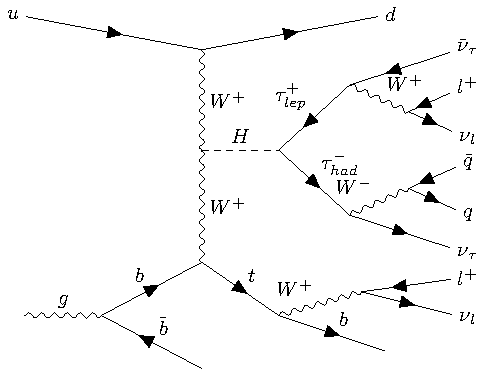
\includegraphics[width=\textwidth]{Feynman_diagrams/Feynman_DileptauGeneralRepresentative_dileptau_SS}
    \caption{\dilepSStau}
    \label{fig:tHq:intro:diltauFeynmanDiagram:SS}
  \end{subfigure}
  \hfill
  \begin{subfigure}[b]{0.45\textwidth}
    \centering
    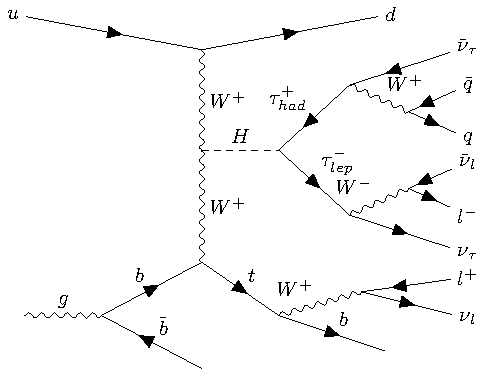
\includegraphics[width=\textwidth]{Feynman_diagrams/Feynman_DileptauGeneralRepresentative_dileptau_OS}
    \caption{\dilepOStau}
    \label{fig:tHq:intro:diltauFeynmanDiagram:OS}
  \end{subfigure}
  \caption{Representative LO Feynman diagrams for the \tHq (\dileptau) in the $\PHiggs \rightarrow \tauhad \taulep$ decay channel.
  Note that the two light leptons in (a) have positive electrical charge and in (b) these leptons have oposite charge.}
  \label{fig:tHq:intro:diltauFeynmanDiagram}
\end{figure}

This chapter is organised as follows: First, in Section \ref{sec:ChaptH:Data_and_MC}, an overview of 
the datasets and MC Ntuples utilised in the analysis is provided. Second, in Section \ref{sec:ChaptH:ObjectDefReco}, 
the particular object definition employed in the analysis is elaborated upon. Section \ref{sec:ChaptH:Sig} delves into various aspects 
of the signal process, including the acquisition of truth-level information, the assignment of light-lepton origin in the 
\dilepSStau channel, and the event reconstruction. In Section \ref{sec:ChaptH:Bkg}, an in-depth description 
of the primary backgrounds encountered during the analysis is presented.
Furthermore, Section \ref{sec:ChaptH:EventSelection} encompasses the signal separation and control region definition, 
accompanied by an outline of the MVA methods employed.
The comprehensive treatment of systematic uncertainties is provided in Section \ref{sec:ChaptH:Systematics}.
Finally, the likelihood fit procedure and the resulting outcomes are presented in Section \ref{sec:ChaptH:Fit}.



%When assuming that one of the light-flavoured leptons is originated from the Higgs-boson decay
%and the other one from the top-quark decay, the determination of which lepton comes from which 
%particle is direct for the \dilepOStau but not for the \dilepSStau. 
%Since knowing the origin of the light-flavoured leptons can be very useful to define variables with
%the power to discriminate the \tHq signal from the background, tools are developed to associate 
%these leptons to its parent particles.

%- The fake rate estimates for light leptons and tau leptons are being checked to see if there is 
%anything that has to be treated differently for the two sub-channels.





%%%%%%%%%%%%%%%%%%%%%%
%           Data and simulated events          %
%%%%%%%%%%%%%%%%%%%%%%
\section{Data and simulated events }
\label{sec:ChaptH:Data_and_MC}
In this section the particularities of the detector real detector data
and the MC generated samples are presented. The generalities 
of the data gathering and the MC samples production are
described in Chapter \ref{chap:DataAndMC}.

All the search channels share the same object selection and use a common set of MC NTuples\cite{SgTopRun2NtuplesContents}, which 
have been produced with the SingleTopAnalysis\footnote{SingleTopAnalysis is
a ROOT-based-software package based on AnalysisTop. It is used to produce
NTuples. AnalsyisTop is the standard analysis software within Athena for Run-2 analysis 
in the Top Working Group.} using the TOPQ1 derivations%\footnote{The derivations were 
%introduced in Section \ref{sec:Chap3.1:Data:Model}. The TopQ1 derivation \pablo{particularidad de topq1¿?}} 
as input \cite{TOPQ}. These TOPQ1 derivations contain a single-lepton filter 
that requires at least one electron or muon that need to satisfy one of the following requirements:
\begin{itemize}
	\item At least one electron with $\abseta \leq 2.5$ and \texttt{Electrons.DFCommonElectronsLHLoose}
	\item Or at least one muon with $\abseta \leq 2.5$ and \texttt{Muons.muonType = 0} and \texttt{Muons.DFCommonGoodMuon}.
\end{itemize}
Additionally this lepton should have $\pT >20\,$GeV or 2015 data and above $25\,$GeV 
for both the 2016--2018 data and the MC simulations.

The produced NTuples have at least two \emu in their final state, one satisfying the condition above and
the other must present a  $\pT >10\,$GeV. \pablo{Do these requirements account for the trigger sensitivity or why this?}

After the NTuples are generated with SingleTopAnalysis, a post-processing framework named \thqloop 
further operates the data samples to skim and slim\footnote{The skimming and slimming are described
in Section \ref{sec:Chap3.1:Data:Model}. The slimming is done by removing unnecessary branches. In ROOT, a branch represents a variable associated with each event or entry in a TTree, which is a hierarchical data structure used for storing and analysing data in the ROOT framework.} them. 
The \thqloop software also to computes additional variables that are needed in the subsequent analysis.





%%%%%%%%%%%%%%%%%%%%%
%                    Data events                      %
%%%%%%%%%%%%%%%%%%%%%
\subsection{Data event samples}
\label{sec:ChaptH:Data_and_MC:Data}
The real data samples used in this analysis correspond to the events
recorded by the ATLAS detector from $\Pproton\Pproton$ collisions with $25\,$ns bunch spacing
delivered by the LHC at $\CM=13\,$TeV during Run\,2. 
This corresponds to a total integrated luminosity of $\lumi^{\text{Run\,2}} = 140\,$fb$^{-1}$.
The uncertainty corresponding to this integrated luminosity has been measured by the LUCID-2
detector to be $0.83\%$. This data-taking period ranges from 2015 to 2018 and for each year
ad different luminosity and uncertainty have been measured, as Table \ref{tab:ChaptH:Data:lumi} shows.

\begin{table}[h]

 \resizebox{\textwidth}{!}{\begin{tabular}{ccccc}
    \toprule
    Year & Periods & Run numbers & Number of events & Integrated luminosity (pb$^{-1})$ \\
    \midrule
    2015 & \dataperiodsFifteen & \datarunsFifteen & \dataeventsFifteen & \lumiFifteenInPbNoUnits\ $\pm$ \lumiFifteenRelUnc\% \\
    2016 & \dataperiodsSixteen & \datarunsSixteen & \dataeventsSixteen & \lumiSixteenInPbNoUnits\ $\pm$ \lumiSixteenRelUnc\% \\
    2017 & \dataperiodsSeventeen & \datarunsSeventeen & \dataeventsSeventeen & \lumiSeventeenInPbNoUnits\ $\pm$ \lumiSeventeenRelUnc\% \\
    2018 & \dataperiodsEightteen & \datarunsEightteen & \dataeventsEightteen & \lumiEightteenInPbNoUnits\ $\pm$ \lumiEightteenRelUnc\% \\
    \midrule
    2015--2018 & All & \firstdatarunFifteen--\lastdatarunEightteen & \dataeventsAll & \lumiInPbNoUnits\ $\pm$ \lumiRelUnc\% \\
    \bottomrule
  \end{tabular}}
  \caption{Total integrated luminosity per year with their relative uncertainties for the Run\,2.
    Additionally, the data-taking periods, run numbers and number of events are shown for each year.}
    \label{tab:ChaptH:Data:lumi}
\end{table}

The good-runs list (GRL) is an xml file that selects the luminosity blocks that are considered good
to be used in an analysis. This is done by demanding that the LHC had stable beams and all
the detectors and subdetectors were operating correctly.
The GRL has been used in order to filter the registered data at the luminosity blocks \footnote{A
luminosity blocks corresponds to about 1 or 2 minutes of data taking and has around $~10^{5}$ events. 
It is a unit of known luminosity.} level. %Source: https://indico.cern.ch/event/472469/contributions/1982677/attachments/1220934/1785823/intro_slides.pdf
Events were selected from a shared data stream using the unprescaled single-lepton triggers, 
which are detailed in Section \ref{sec:ChaptH:ObjectDefReco:trigger}.


%%%%%%%%%%%%%%%%%%%%%
%                Simulated events                  %
%%%%%%%%%%%%%%%%%%%%%
\subsection{Simulated event samples}
\label{sec:ChaptH:Data_and_MC:MC}
The event samples used in the analysis were generated using MC 
simulations with different event generators and simulation frameworks. 
The generalities of the ATLAS simulation chain are described in 
Section \ref{sec:Chap3.1:MC}.

The MC production is divided into campaigns, where the centre-of-mass energy,
geometry and conditions used in production correspond to a running period of
the LHC.  Major campaigns align with calendar years, such as mc15 and mc16, 
while minor campaign versions often indicate updates or enhancements in 
reconstruction software, trigger menus, or pile-up simulation, denoted by 
designations like mc15a, mc16b, and so on.
The MC16a/d/e production campaigns were employed, which involved various event generators interfaced with shower/hadronisation generators. 

% PMG: Physics Modelling Group
% APG: ATLAS MC Prodduction Group

After the event generation, the trigger and detector simulation were 
performed using the Athena.
The detector simulation was carried out either using the GEANT4 framework \cite{GEANT4:2002zbu} 
for a detailed physics description or the \texttt{Atlfast2} \cite{SOFT-2010-01}
(AFII) framework for 
faster simulation. The AFII framework uses a parametric cell response for the ATLAS
calorimeters, while GEANT4 is used for the rest of the simulation. 

In the analyses, full-simulated (FS) event samples were used as the baseline whenever 
available. For certain cases such as the \tHq signal process and the \tHW
and four top-quark background processes, AFII event samples were used as baseline.
Most of the systematic effects were evaluated using AFII samples, except for 
specific systematic uncertainties such as \ttbar/\tW interference, \ttZ, \ttW, and \tWZ 
modelling, where FS event samples were used.

The effect of multiple interactions within the same and neighbouring 
bunch crossings, i.e. \pileup, was incorporated by overlaying the hard-scattering event 
with inelastic \pp\ events generated using \PYTHIA[8.186]\cite{Sjostrand:2007gs}. 
The ATLAS third set of tuned parameters for minimum-bias events (A3 tune\cite{ATL-PHYS-PUB-2016-017}) 
and the \NNPDF[2.3lo] set of PDFs\cite{Ball:2012cx} were employed for the \pileup modelling.

The MC events were weighted to match the distribution of the average number of interactions per bunch crossing \(\left<\mu \right>\) observed in the data. A rescaling factor of \(1.03\pm 0.04\) was applied to the data's $\left<\mu \right>$ value to improve agreement between data and simulation in the visible inelastic \pp\ cross-section\cite{STDM-2015-05}.

These samples were used to assess efficiency and resolution models and to estimate 
systematic uncertainties. The details of each simulation event sample for each process 
are provided in the subsequent subsections.
 A summary of all \tHq signal and background processes 
is presented in Table \ref{tab:ChaptH:Data_and_MC:MCsummary}. 
The relevance of the processes 
listed in Table \ref{tab:ChaptH:Data_and_MC:MCsummary} is not uniform.
 In this section,  we discuss the significance of each background process, highlighting their respective importance and in Section \ref{sec:ChaptH:Bkg} the estimation
 of the yields is presented.  


\pablo{En esa sección hay que explicar con detalle como se modela la señal y luego explicar también
los principales fondos. El resto se ponen como minor backgrounds y se añade una tabla resumen de todos
los procesos.}


\begin{table}[!htbp]  
  \begin{adjustbox}{max width=0.99\textwidth}
    \begin{tabular}{llllll}
      \toprule
      Process & Generator & Order (scheme) & PDF set & Parton shower & PDF set (tune) \\
      \midrule
      \multicolumn{6}{c}{Signal} \\
      \midrule
      \tHq & \MGNLO[2.6.2] & NLO (4FS) & \NNPDF[3.0nlo] nf4 & \PYTHIA[8.230] & \NNPDF[2.3lo] (A14 tune) \\
      \midrule
      \multicolumn{6}{c}{Backgrounds} \\
      \midrule
      \ttbar & \POWHEGBOX[v2] & NLO (5FS) & \NNPDF[3.0nlo] & \PYTHIA[8.230] & \NNPDF[2.3lo] (A14 tune) \\
      \(V\)+jets & \SHERPA[2.2.1] & NLO+LO & \NNPDF[3.0nnlo] & - & - \\
      \Diboson & \SHERPA[2.2.1-2] & NLO+LO & \NNPDF[3.0nnlo] & - & -\\
      \Triboson & \SHERPA[2.2.2] & NLO+LO & \NNPDF[3.0nnlo] & - & - \\
      \ttZ & \MGNLO[2.3.3] & NLO & \NNPDF[3.0nlo] & \PYTHIA[8.210] & \NNPDF[2.3lo] (A14 tune) \\
      \ttW & \SHERPA[2.2.10] & NLO & \NNPDF[3.0nnlo] & - & - \\
      %\ttV & \MGNLO[2.3.3] & NLO & \NNPDF[3.0nlo] & \PYTHIA[8.210] & \NNPDF[2.3lo] (A14 tune) \\
      \ttH & \POWHEGBOX[v2] & NLO (5FS) & \NNPDF[3.0nlo] & \PYTHIA[8.230] & \NNPDF[2.3lo] (A14 tune) \\
      \(t\)-channel & \POWHEGBOX[v2]  & NLO (4FS) & \NNPDF[3.0nlo] nf4 & \PYTHIA[8.230] & \NNPDF[2.3lo] (A14 tune) \\
      \Wt & \POWHEGBOX[v2] & NLO (5FS, DR) & \NNPDF[3.0nlo] & \PYTHIA[8.230] & \NNPDF[2.3lo] (A14 tune) \\
      \(s\)-channel & \POWHEGBOX[v2] & NLO & \NNPDF[3.0nlo] & \PYTHIA[8.230] & \NNPDF[2.3lo] (A14 tune) \\
      \tZq & \MGNLO[2.3.3] & NLO & \NNPDF[3.0nlo] & \PYTHIA[8.230] & \NNPDF[2.3lo] (A14 tune) \\
      \tHW{} & \MGNLO[2.8.1] & NLO (5FS, DR) & \NNPDF[3.0nlo] & \PYTHIA[8.245p3] & \NNPDF[2.3lo] (A14 tune) \\
      \tWZ & \MGNLO[2.3.3] & NLO & \NNPDF[3.0nlo] & \PYTHIA[8.212] & \NNPDF[2.3lo] (A14 tune) \\
      \ttt & \MGNLO[2.2.2] & NLO & \NNPDF[3.1nlo] & \PYTHIA[8.186] & \NNPDF[2.3lo] (A14 tune) \\
      \tttt & \MGNLO[2.3.3] & NLO & \NNPDF[3.1nlo] & \PYTHIA[8.230] & \NNPDF[2.3lo] (A14 tune) \\
      \ggH & \POWHEGBOX[v2] & NLO & \CT[10] & \PYTHIA[8.210] & \CTEQ[6L1] (\AZNLO tune) \\
      \qqH & \POWHEGBOX[v1] & NLO & \CT[10] & \PYTHIA[8.186] & \CTEQ[6L1] (\AZNLO tune) \\
      \WH & \PYTHIA[8.186] & LO & \NNPDF[2.3lo] & - & - \\
      \ZH & \PYTHIA[8.186] & LO & \NNPDF[2.3lo] & - & - \\
      \bottomrule
    \end{tabular}
  \end{adjustbox}
  \caption{Summary of the baseline simulated signal and background event
    samples used in the \tHq analyses.}
  \label{tab:ChaptH:Data_and_MC:MCsummary}
\end{table}

%%%%%%%%%%%%%%%%%%%%%
%                Simulated signal                  %
%%%%%%%%%%%%%%%%%%%%%
\subsubsection{Simulated \tHq signal samples}
\label{sec:ChaptH:Data_and_MC:MC:Sig}
The \tHq event sample was generated using the \MGNLO[2.6.2]\cite{Alwall:2014hca} 
generator at NLO, employing the \NNPDF[3.0nlo] nf4\cite{Ball:2014uwa} PDF set. The 
events were then interfaced with \PYTHIA[8.230]\cite{Sjostrand:2014zea} using the 
A14\cite{ATL-PHYS-PUB-2014-021} tune and the \NNPDF[2.3lo] PDF set. The 
renormalisation (\muR) and factorisation scales (\muF) were set to a default scale 
based on the momenta of the particles generated from the matrix element calculation.

Alternative samples of simulated \tHq signal events were produced using the 
\MGNLO[2.8.1] generator at NLO with the \NNPDF[3.0nlo] nf4 PDF set, and interfaced 
with \HERWIG[7.1.6] using the \MMHT[nnlo]\cite{Harland-Lang:2014zoa} PDF set and the 
\HERWIG[7.1]\cite{Bahr:2008pv}\cite{Bellm:2015jjp} tune. The scales \muR and \muF 
were the same as for the nominal \tHq event sample.

Additionally, samples of simulated \tHq signal events with the inverted Yukawa coupling 
hypothesis ($\yt=-1$) were produced using either the \MGNLO[2.6.2] and 
\MGNLO[2.8.1] generators at NLO with the \NNPDF[3.0nlo] nf4 PDF set, and interfaced 
with either \PYTHIA[8.230] or \PYTHIA[8.245], both using the A14 tune and the 
\NNPDF[2.3lo] PDF set. The \muR and \muF scales were also the same as for the nominal 
event sample.

To account for higher and lower parton radiation, the \muR and \muF scales were varied 
by factors of 0.5 and 2. The variations used are $\{\muR, \muF\} = \{0.5,0.5\}, \{1,0.5\}, \{0.5,1\}, \{1,1\}, \{2,1\}, \{1,2\}, \{2,2\}$. 
These variations were included in the nominal samples as additional weights. The final 
uncertainty was estimated by taking the envelope of all the uncertainties associated with 
each variation, as it is recommended by the Physics Modelling 
Group\cite{PmgSystematicUncertaintyRecipes}.

The simulation event samples were generated in the 4FS scheme (see Section 
\ref{sec:Chap1:Top:Production:SingleTop} for FS discussion). The top quark decay was 
simulated at LO using \MADSPIN\cite{Frixione:2007vw}\cite{Artoisenet:2012st} to preserve 
spin correlations, while the decay of the Higgs boson was generated either by \PYTHIA[8] 
or \HERWIG[7] in the parton shower. The decays of bottom and charm hadrons were 
simulated using either \EVTGEN[1.6.0] or \EVTGEN[1.7.0]\cite{Lange:2001uf}.


The normalisation of the \tHq signal samples was performed with respect to the cross-section predictions obtained from \MGNLO at NLO. For proton-proton collisions at
$\CM = \sqrt{13}\,$TeV, the cross-section correspond to $\sigma(\tHq(ML))_{\text{NLO}} = 16.7\,$fb, 
using a top-quark mass of $\mtop =172.5\,$GeV. $\tHq (ML)$ refers
to the multi-leptonic channels, in contrast to the $\tHq(\bbbar)$ with a cross section of 
$\sigma(\tH(\bbbar))_{\text{NLO}} = 60.1\,$fb.


%%%%%%%%%%%%%%%%%%%%%
%           Simulated background               %
%%%%%%%%%%%%%%%%%%%%%
\subsubsection{Simulated background samples}
\label{sec:ChaptH:Data_and_MC:MC:Bkg}
%%%%
%Define what background 
%%%%
The background can be defined as everything in a subset of the data that 
imitates the signal processes without truly being a signal event.  Therefore, 
in this study, whatever that mimics the signature of an associated \tHq production 
with  \dileptau final state is referred as background. 
%In other words, in this study, everything that is not the signal \tHq, is background.

%%%%
%Why is important to discriminate it. % http://www.thomasgmccarthy.com/an-introduction-to-collider-physics-ix
%%%%
In order to perform the physics analysis, it is fundamental to subtract the background events from the dataset
as much as possible in order to achieve higher signal purity.
By doing this, the analysed dataset resembles more to the process that is desired to study.
This procedure is the so called ``event selection'' and its described in Section \ref{sec:ChaptH:EventSelection}.

%%%%
% Classification in Reducible and Irreducible bkgs
%%%%
In our analysis, we classify background events into two distinct types:  
``reducible'' backgrounds and ``irreducible'' backgrounds.

Reducible backgrounds refer to situations where particles in the event 
simulation mimic the characteristics of the particles we are specifically 
interested in. For example, a high-energy electron can produce a signature 
that closely resembles that of a high-energy photon, leading to misidentification.

On the other hand, irreducible backgrounds involve physical objects that are of 
the same nature as the particles we are targeting. These backgrounds cannot be 
easily distinguished from our signal events based on their properties alone.


In the \dileptau channel, the dominant backgrounds consist of reducible events 
where jets misidentified as \tauhad are present. This is particularly observed in 
the \ttbar and \Zjets backgrounds. Additionally, other backgrounds include processes 
involving dibosons (\diboson) and associated top quark production (\ttX), such 
as \ttH, \ttZ, and \ttW.

When considering events with a same-sign lepton pair, all background contributions 
are significantly reduced compared to the opposite-sign case. Nevertheless, the dominant 
background remains \ttbar, followed by the \ttX processes, as indicated in Table \ref{tab:ChaptH:EventSelection:Preselection}.

In the \dileptau channel, the primary source of background arises from hadronic 
tau decays, particularly cases where jets falsely resemble \tauhad signatures.
%While this type of backgrounds are discussed in section \ref{sec:ChaptH:Bkg:Fakes},
%the irreducible backgrounds are presented in Section \ref{sec:ChaptH:Bkg:Irreducible}.



\begin{table}[]
\centering
\begin{tabular}{l| l| l| l}
\toprule
Process      & \dilepSStau     & \dilepOStau     & \dileptau \\ \midrule
\tHq          & 0.9    & 1.2    & 2.1     \\
\tZq  (with $\PZ \rightarrow \Plepton \Plepton$)        & 6.2    & 32.9   & 39.1    \\ % This is not actually tZq but just tllq :: Associated production of top and Z where the Z decays into leptons (including taus)
\ttbar           & 47.9   & 2965.0 & 3012.9  \\
\tW           & 2.3    & 118.9  & 121.2   \\
\PW+jets       & 1.9    & 0.5    & 2.4     \\
\PZ+jets       & 6.7    & 1956.2 & 1962.9  \\
VV + jets (V$=\PW / \PZ$)      & 8.9    & 121.6  & 130.5   \\
\ttW          & 21.0   & 43.4   & 64.4    \\
\ttZ          & 17.5   & 101.2  & 118.7   \\
\ttH          & 17.8   & 43.2   & 61.0    \\
\tWZ   (with $\PZ \rightarrow \Plepton \Plepton$)       & 3.1    & 16.4   & 19.5    \\
\tWH          & 0.6    & 1.5    & 2.1     \\
Other        & 1.9    & 9.3    & 11.2    \\ \midrule
Total        & 136.7  & 5411.3 & 5548.0  \\ \midrule
\StoB (\%)     & 0.6627 & 0.0222 & 0.0379  \\ \midrule
Significance & 0.0771 & 0.0163 & 0.0282 \\
 \bottomrule
\end{tabular}
\caption{Event yields at preselection level for \dileptau channel and its two subchannels.\pablo{The \PW and \PZ MC only feature leptonic decays. Must update with latest results.}}
\label{tab:ChaptH:EventSelection:Preselection}
\end{table}



In the subsequent section, the MC simulation of the background processes 
is discussed, highlighting their specific characteristics. Furthermore, an 
explanation is provided for each of these processes to elucidate who they contribute
to the background. Later on, in Section \ref{sec:ChaptH:Bkg} of the thesis, a 
comprehensive description of the background estimation will be presented, offering 
detailed insights into the methodologies employed.

\pablo{En estas subsecciones he de describir por qué cada uno de estos procesos es considerado como fondo. De qué forma imitan la signatura de \tHq.}

%%%%%
% ttbar %
%%%%%
\paragraph{Top quark pairs}\mbox{}\\
The production of top-quark pair (\ttbar) events constitute the main background source
for both \dileptau channels. Figure \ref{fig:tHq:Backgrounds:Feynman_ttbar} presents
a \ttbar production Feynman diagram in which the top quarks decay leptonically. 
When these leptons are electrons or muons, the \ttbar process can mimic the
\dilepOStau signature if one of the quarks is wrongly reconstructed as an hadronically
decaying tau. As it is discussed in Section \ref{sec:ChaptH:Bkg:Fakes}, the misidentification of quarks as if they were \tauhad constitutes the main source of background.
If one of the leptons in the \ttbar diagram was an hadronically-decaying tau and the other an \emu, the 
\dileptau signature could be obtained if one of the \bjets is wrongly identified as an \emu. This second scenario is less common but can still happen.

\begin{figure}[htbp!]
\centering
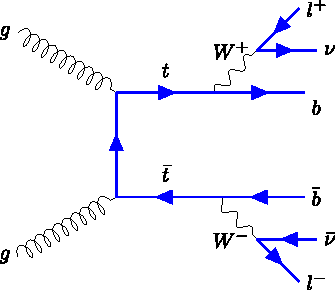
\includegraphics[width=.5\textwidth]{Feynman_diagrams/Vectorial_Backgrounds/Feynman_ttbar_Vectorial}
\caption{LO Feynman diagram for the \ttbar process, the main background. 
	In this particular diagram both \PW bosons decay leptonically.}
\label{fig:tHq:Backgrounds:Feynman_ttbar}
\end{figure}

\pablo{The description of \ttbar generations seems too technical.}

Regarding its generation, the \ttbar events have been simulated using 
\POWHEGBOX[v2] \cite{Frixione:2007nw, Nason:2004rx, Frixione:2007vw, Alioli:2010xd},
 which incorporates NLO MEs in the strong coupling constant \alphas, and the 
 \NNPDF[3.0nlo] PDF set \cite{Ball:2014uwa}. The parameter \hdamp, controlling 
 the matching between the \POWHEG generator and high-\pT radiation, was set to 
 $1.5\times\mtop$~\cite{ATL-PHYS-PUB-2016-020}.
The \muR  and \muF scales were set to the default scale of \(\sqrt{\mtop^{2} + \pT^{2}}\).

The subsequent PS and hadronisation processes were performed using \PYTHIA[8.230], 
adopting the A14 tune and the \NNPDF[2.3lo] PDF set. %In this context, the presented 
%analyses utilized a non-all-hadronic filtered simulation sample with the dataset identifier 
%(DSID) 410470.
The impact of using a different PS and hadronisation model was evaluated
by comparing the nominal \ttbar sample with an event sample also produced with the
\POWHEGBOX[v2] generator but interfaced with \HERWIG[7.13], using the
\HERWIG[7.1] tune and the
\MMHT[lo] PDF set. \POWHEGBOX provided MEs at NLO in the \alphas, and used the
\NNPDF[3.0nlo] PDF set and
an \hdamp parameter value of $1.5\times\mtop$.



The uncertainty due to initial-state radiation (ISR) was estimated 
by comparing the nominal \ttbar events using the A14 tune with \ttbar events with the same 
settings as the nominal ones, but employed the \texttt{Var3c up} or \texttt{down} variation 
of the A14 tune, which corresponds to the variation of \alphas for ISR in the A14 
tune\cite{ATL-PHYS-PUB-2014-021}. The uncertainty due to final-state radiation (FSR) 
was evaluated by varying the \muR scale for emissions from the PS up and down by a 
factor of two.

A variation of the \hdamp parameter was considered by comparing the nominal with 
alternative event samples with $\hdamp = 3.0\mtop$.

All these samples were generated in the 5FS and top quarks were decayed at LO using 
\MADSPIN \cite{Frixione:2007zp,Artoisenet:2012st} to preserve spin correlations. The 
decays of bottom and charm hadrons were simulated using the \EVTGEN[1.6.0] program.

The \ttbar sample was normalised to the cross-section prediction at NNLO
in QCD including the resummation of NNLL soft-gluon terms calculated using
\TOPpp[2.0]~\cite{Beneke:2011mq,Cacciari:2011hy,Baernreuther:2012ws,Czakon:2012zr,Czakon:2012pz,Czakon:2013goa,Czakon:2011xx}.
For \pp\ collisions at \(\rts = 13\,\)TeV, this cross-section corresponds to
\(\sigma(\ttbar)_{\text{NNLO+NNLL}} = 832 \pm 51\,\)fb using a top-quark mass of \(\mtop = 172.5\,\)GeV.
The uncertainties in the cross-section due to the PDF and \alphas were calculated using 
the \PDFforLHC[15] prescription~\cite{Butterworth:2015oua}
with the \MSTW[nnlo]~\cite{Martin:2009iq,Martin:2009bu}, 
\CT[10nnlo]~\cite{Lai:2010vv,Gao:2013xoa}
and \NNPDF[2.3lo] PDF sets in the 5FS, and were
added in quadrature to the effect of the scale uncertainty.


%%%%%
% Zjets %
%%%%%
\paragraph{Single boson}\mbox{}\\
This background corresponds to the \PZ+jets and \PW+jets productions, which where
 simulated with \Sherpa generator and \NNLO. 
 
 
 \begin{figure}[htbp!]
\centering
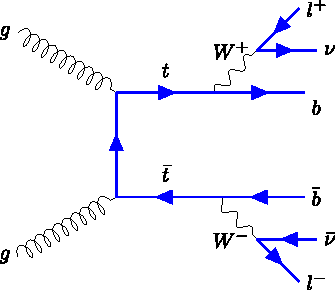
\includegraphics[width=.5\textwidth]{Feynman_diagrams/Vectorial_Backgrounds/Feynman_ttbar_Vectorial}
\caption{Representative LO Feynman diagram for the \Zjets process, the second most dominant background. In this particular case, the \PZ boson decays leptonically and
the gluon splits into a \bbbar pair.}
\label{fig:tHq:Backgrounds:Feynman_Zjets}
\end{figure}
 
%%%%%%%
% Diboson %
%%%%% %%
\paragraph{Diboson}\mbox{}\\
Diboson

\begin{figure}
\centering
\begin{subfigure}[b]{0.45\textwidth}
   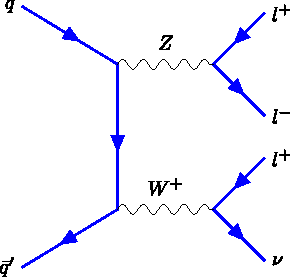
\includegraphics[width=1\linewidth]{Feynman_diagrams/Vectorial_Backgrounds/Feynman_Diboson_ZW_Vectorial}
   \caption{$\PW \PZ$}
   \label{fig:tHq:Backgrounds:Feynman_Diboson:WZ}
\end{subfigure}
\begin{subfigure}[b]{0.45\textwidth}
   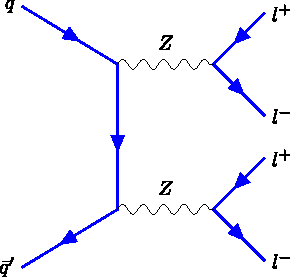
\includegraphics[width=1\linewidth]{Feynman_diagrams/Vectorial_Backgrounds/Feynman_Diboson_ZZ_Vectorial}
   \caption{$\PZ \PZ$}
   \label{fig:tHq:Backgrounds:Feynman_Diboson:WW}
\end{subfigure}
\caption{Representative LO Feynman diagram for the Diboson processes.}
\label{fig:tHq:Backgrounds:Feynman_Diboson}
\end{figure}

%%%%%%%
% triboson %
%%%%%%%
\paragraph{Triboson}\mbox{}\\

%%%%%
% ttV %
%%%%%
\paragraph{Top-quark pair + single-boson}\mbox{}\\

\begin{figure}[htbp!]
\centering
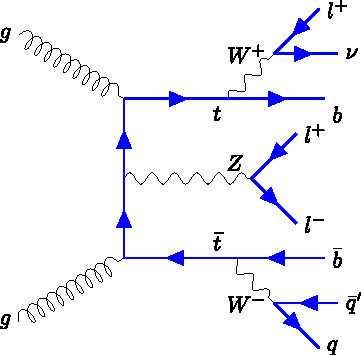
\includegraphics[width=.5\textwidth]{Feynman_diagrams/Vectorial_Backgrounds/Feynman_tt+X_Vectorial}
\caption{Representative LO Feynman diagram for the \ttZ}
\label{fig:tHq:Backgrounds:Feynman_ttZ}
\end{figure}




\paragraph{Top-quark pair + Higgs-boson }\mbox{}\\
\paragraph{Single top-quark: \tchannel}\mbox{}\\
\paragraph{Single top-quark: \tW associated production}\mbox{}\\
\paragraph{Single top-quark: \schannel}\mbox{}\\


\paragraph{Single top-quark $+X$: \tZq}\mbox{}\\
\begin{figure}[htbp!]
\centering
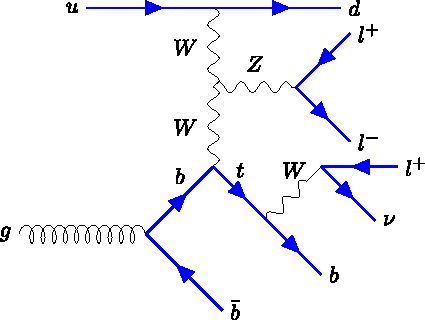
\includegraphics[width=.5\textwidth]{Feynman_diagrams/Vectorial_Backgrounds/Feynman_tZq_Vectorial}
\caption{Representative LO Feynman diagram for the \tZq}
\label{fig:tHq:Backgrounds:Feynman_tZq}
\end{figure}



\paragraph{Single top-quark $+X$: \tWH}\mbox{}\\
\paragraph{Single top-quark $+X$: \tWZ}\mbox{}\\

\paragraph{Single top-quark $+X$: \tZq}\mbox{}\\
\begin{figure}[htbp!]
\centering
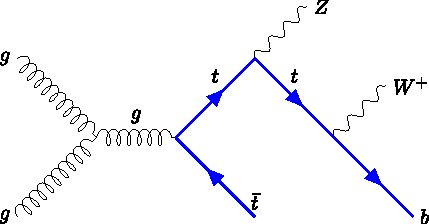
\includegraphics[width=.5\textwidth]{Feynman_diagrams/Vectorial_Backgrounds/Feynman_tWZ_Vectorial}
\caption{Representative LO Feynman diagram for the \tWZ}
\label{fig:tHq:Backgrounds:Feynman_tWz}
\end{figure}


\paragraph{Three top-quark}\mbox{}\\
\paragraph{Higgs boson process}\mbox{}\\
% the tH samples were done with \MGNLO+\PYTHIA[8]+\EVTGEN


%The underlying event is generally done with Pythia8 in ATLAS. In the tHq samples we used \MGNLO for the calculation of the matrix element and \PYTHIA[8] for the hadronisation and parton showering. We are also working on alternative samples with \Herwig[7] as parton shower generator.
%\pablo{While in section 3 I describe how the events and samples are generally generated and simulated, in this section I should describe what is specifically used in this analysis}




%%%%%%%%%%%%%%%%%%%%%%%%%%
%           Object definition and reconstruction         %
%%%%%%%%%%%%%%%%%%%%%%%%%%
\section{Object definition}
\label{sec:ChaptH:ObjectDefReco}
In Chapter \ref{chap:ObjectReconstuction}, a general overview of the object 
reconstruction process was provided. Various definitions were employed for 
each of the physical objects. This section focuses on discussing the specific 
definitions employed for this analysis at hand.


\pablo{Highlight the importance of alignment somwhere}

%The \antikt algorithm with a radius parameter of \(R=0.4\) is used to reconstruct jets with a four-momentum recombination scheme, using \topos as inputs. Jet energy is calibrated to the hadronic scale with the effect of \pileup removed

%Hadronic jets are reconstructed from calibrated three-dimensional \topos.
%Clusters are constructed from calorimeter cells that are grouped together using a topological clustering algorithm.
%These objects provide a three-dimensional representation of energy depositions in the calorimeter and implement a nearest-neighbour noise suppression algorithm.
%The resulting \topos are classified as either electromagnetic or hadronic based on their shape, depth and energy density.
%Energy corrections are then applied to the clusters in order to calibrate them to the appropriate energy scale for their classification.
%These corrections are collectively referred to as \textit{local cluster weighting}, or LCW, and jets that are calibrated using this procedure are referred to as LCW jets~\cite{PERF-2012-01}.}

%
% Triggers
%
\subsection{Triggers}
\label{sec:ChaptH:ObjectDefReco:trigger}
To select events from collisions, a two-level trigger system is employed, as documented in~\cite{TRIG-2016-01} and 
described in Section \ref{sec:Chap2:Trigger_and_DAQ}. 
The L1 operates through hardware and utilises partial detector information to decrease the rate of accepted events from 
the interaction frequency of $40\,$MHz to $100\,$kHz. The HLT, on the other hand, is software-based and accepts 
events at a rate of $1\,$kHz.

During the data-taking period spanning 2015--2018, varying pile-up conditions necessitated the use of different single-lepton 
(electron or muon) triggers, which were not subjected to prescaling~\cite{LowestUnprescaled}. The trigger names employed 
in this analysis are listed in Table \ref{tab:ChaptH:ObjectDefReco:Triggers}. These triggers are combined using a logical 
\texttt{OR} operation.

\begin{table}[!htbp]
  \begin{adjustbox}{max width=0.99\textwidth}
    \begin{tabular}{c|ll}
      \toprule
      Year & Single-electron trigger & Single-muon trigger \\
      \midrule
           & \texttt{HLT\_e24\_lhmedium\_L1EM20VH} & \texttt{HLT\_mu20\_iloose\_L1MU15} \\
      \datafirstyear\ & \texttt{HLT\_e60\_lhmedium} & \texttt{HLT\_mu50} \\
           & \texttt{HLT\_e120\_lhloose} & \\
      \midrule
           & \texttt{HLT\_e26\_lhtight\_nod0\_ivarloose} & \texttt{HLT\_mu26\_ivarmedium} \\
      2016--\datalastyear\ & \texttt{HLT\_e60\_lhmedium\_nod0} & \texttt{HLT\_mu50} \\
           & \texttt{HLT\_e140\_lhloose\_nod0} & \\
      \bottomrule
    \end{tabular}
  \end{adjustbox}
    \caption{Employed single-lepton trigger depending on the light-lepton flavour and year.
    These individual single-lepton triggers are combined using a logical \texttt{OR} operation.}
  \label{tab:ChaptH:ObjectDefReco:Triggers}
\end{table}
% https://twiki.cern.ch/twiki/bin/view/AtlasProtected/TopqTriggers
% https://twiki.cern.ch/twiki/bin/viewauth/Atlas/TrigGlobalEfficiencyCorrectionTool#Supported_trigger_combinations

%Electron triggers
The electron triggers in this analysis employ a selection criteria that involves matching a calorimeter cluster to a track. 
Subsequently, electrons are required to meet identification criteria utilising a multi-variate technique with a likelihood discriminant.
Depending on the year, the single-electron triggers utilised in this analysis are as follows:
\begin{itemize}
	\item In \datafirstyear, electron triggering involved requiring a transverse energy deposit (\ET) above $20\,$GeV at the L1. 
	At the HLT, the full calorimeter granularity and tracking information were considered, and the reconstructed calorimeter
	cluster was matched to a track. The trigger electron object was required to be isolated, with a \texttt{medium} identification 
	according to the criteria described in Section \ref{sec:ChaptH:ObjectDefReco:electron}, and have $\ET > 24\,$GeV.
	\item In the years 2016--2018, the electron triggers required electrons to satisfy a \texttt{tight} identification at the HLT, 
	along with an isolation criterion, and have an $\ET > 26\,$GeV.
	\item Two complementary triggers were employed throughout Run$\,$2 to mitigate efficiency losses at high \pT, 
	in addition to the previous triggers. These triggers either selected \texttt{medium} electrons with $\ET > 60\,$GeV 
	at the HLT or selected \texttt{loose} electrons with $\ET > 120\,$GeV in 2015 and 
	$\ET > 140\,$GeV in 2016--2018. By \texttt{loose} its meant that no isolation requirements were demanded.
\end{itemize}

%Muon triggers
Muons in this analysis are triggered by matching tracks reconstructed in both the MS and ID.
In \datafirstyear, the muon triggers required muons to satisfy a loose isolation requirement and
have a \pT greater than $20\,$GeV. In the years 2016--2018, the isolation criterion was tightened, 
and the threshold was increased to $\pT > 26\,$GeV.
Similar to the electron triggers, to mitigate efficiency losses due to isolation at high \pT, an additional 
muon trigger without any isolation requirement was available throughout all these years. 
This trigger selected loose muons with $\pT > 50\,$GeV.

%
% Electrons
%
\subsection{Electrons}
\label{sec:ChaptH:ObjectDefReco:electron}
The requirements for preselected electrons used in the overlap removal process\footnote{The 
overleap removal vetoes physics objects in the event with reconstruction ambiguities that can lead 
to double-counting.  It is described in Section \ref{sec:ChaptH:ObjectDefReco:OverlapRemoval}}
and electrons selected for the analysis are summarised in left column of 
the Table \ref{tab:ChaptH:ObjectDefReco:Electrons_Muons}.
The recommendation is the use of likelihood-based electron identification 
techniques \cite{PERF-2017-01,EGAM-2018-01} due to their improved 
background rejection compared to cut-based electron identification. 
Different working points are supported, which correspond to different levels 
of efficiency in identifying prompt electrons and rejection of non-prompt electrons. 
For pre-selected electrons, a \texttt{looseAndBLayerLH} identification is applied.
%On the other hand, for electrons selected in one of the analysis regions, a \texttt{tightLH} 
%identification is required.
These electrons must satisfy the following criteria: $\pT > 10,$GeV and $|\eta| < 2.47$. 
Additionally, a requirement on electron isolation is imposed, which corresponds to the 
\texttt{PLImprovedTight} (Prompt Lepton Improved Veto) isolation working 
point \cite{twiki-IFF,twiki-ISOWP,PLIV}. This isolation working point is defined by a 
multivariate likelihood discriminant that combines shower shape and track information 
to distinguish prompt electrons from electron candidates originating from hadronic jets, 
photon conversions, and decays of heavy-flavour hadrons.

The reconstructed track associated with the electron must satisfy: $|\zzsth| < 0.5\,$mm 
and $|\dzero| / \sigma(\dzero) < 5$. Here, $z_{0}$ represents the longitudinal impact 
parameter relative to the reconstructed primary vertex, where the primary vertex is 
defined as the vertex with the highest scalar sum of the squared transverse momenta 
of associated tracks with $\pt > 400\,$MeV. \dzero corresponds to the transverse impact 
parameter relative to the beam axis, and $\sigma(\dzero)$ denotes the uncertainty on \dzero.
Electron candidates are excluded if their calorimeter clusters lie within the transition region 
between the barrel and the endcap of the electromagnetic calorimeter, defined as 
$1.37 < |\eta^\mathrm{clust}| < 1.52$. To account for the efficiency differences between data 
and simulation when applying these requirements, associated scale factors (SFs) for electron r
econstruction, identification, and isolation are applied in Monte Carlo (MC) simulations \cite{egammaRecommendations}.

In certain analysis regions, additional requirements are imposed on electrons. These include the application of 
the \enquote{Electron Charge ID Selector Tool} (ECIDS) \cite{twiki-ECIDS}, which enhances the rejection of electrons 
with misidentified electrical charges. Moreover, for specific regions, cuts on the \texttt{DFCommonAddAmbiguity} 
and \texttt{ambiguityType} variables are implemented, as defined by the \enquote{Electron Ambiguity Tool} in 
the E/gamma derivation framework \cite{twiki-elAmbiguity}. These cuts are designed to suppress the contribution 
from electrons originating from photon conversions by removing objects with multiple reconstructed tracks in close 
proximity to the calorimeter cluster.
It is worth noting that the requirement \enquote{$\texttt{ambiguityType} = 0$} in conjunction 
with \enquote{$\texttt{DFCommonAddAmbiguity} \leq 0$} signifies the selection of electrons with a 
veto on internal/material photon conversion candidates. In the following discussion, this will be referred 
to as the \enquote{$e/\gamma$ ambiguity-cuts}.

\pablo{The information in subsection \ref{sec:ChaptH:ObjectDefReco:electron} has been taken from the int-note. Maybe it is too technical.}
 
%
% Muons
%
\subsection{Muons}
\label{sec:ChaptH:ObjectDefReco:muon}
The selection criteria for muons are summarized in the right column of Table \ref{tab:ChaptH:ObjectDefReco:Electrons_Muons}.
Preselected muons, used for the overlap removal process, must satisfy: $\pt > 7\,$GeV, $|\eta| < 2.5$, 
and the \texttt{medium} identification criteria recommended by the muon CP group \cite{MCPRecommendations}. 
This working point imposes conditions on the number of hits in the ID and MS subsystems, as well as 
on the significance of the charge-to-momentum ratio ($q/p$) \cite{PERF-2015-10}\cite{MUON-2018-03}. 
If a muon is flagged as \enquote{bad} due to insufficient momentum resolution, the entire event is removed,
following the recommendations from the muon CP group \cite{twiki-MuonSelection}.
In addition to the criteria for preselected muons, muons selected for analysis regions are subject 
to the \texttt{PLImprovedTight} isolation requirement. This isolation criterion is applied to suppress 
contributions from fake or non-prompt muons \cite{twiki-IFF}\cite{twiki-ISOWP}\cite{PLIV}.

The recommended cuts for the longitudinal impact parameter (IP) and transverse 
impact parameter (d0) are applied to muon candidates. The reconstructed track 
associated with the muon must satisfy $|\zzsth| < 0.5\,$mm and $|\dzero| / \sigma(\dzero) < 3$. 
SFs for muon identification and isolation are applied as multiplicative factors to the MC event weight. 
These SFs correct for the differences in efficiency between data and MC simulations. 
The details of these corrections can be found in the references \cite{MCPRecommendations}\cite{PERF-2015-10}.
\pablo{Check if IP and d0 have been already defined}

\pablo{Change "recommendations from the CP group" by just "recommendations".}


\begin{table}[!htbp]
  \begin{tabular}{ l|l|l }
    \toprule
    & \multicolumn{1}{c|}{Pre-selected electron} & \multicolumn{1}{c}{Pre-selected muon} \\
    \midrule
    Identification   & \multicolumn{1}{c|}{\texttt{looseAndBLayerLH}} & \multicolumn{1}{c}{\texttt{medium}} \\
    Acceptance       & $\pt > 10\,$GeV, $|\eta^\mathrm{clust}| < 2.47$  & $\pt > 10\,$GeV, $\abseta < 2.5$ \\
                     &  except $1.37 < |\eta^\mathrm{clust}| < 1.52$          & \\
    Impact parameter & $|\dzero/\sigma(\dzero)| < 5.0$                   & $|\dzero/\sigma(\dzero)| < 3.0$ \\
                     & $|\zzsth| < 0.5\,$mm                      & $|\zzsth| < 0.5\,$mm \\
     Overlap removal & \multicolumn{2}{c}{See Section \ref{sec:ChaptH:ObjectDefReco:OverlapRemoval}} \\
    \bottomrule
    & \multicolumn{1}{c|}{Electron} & \multicolumn{1}{c}{Muon} \\
    \midrule
    Identification   & \multicolumn{1}{c|}{\texttt{tightLH}} &  \multicolumn{1}{c}{\texttt{medium}}\\
    Isolation        & \texttt{PLImprovedTight}  & \texttt{PLImprovedTight} \\
    Extra selections & ECIDS, $e/\gam$ ambiguity-cuts &  \\
    \bottomrule
  \end{tabular}
  \caption{Summary of the electron and muon object definitions. The selection requirements for actual
          electrons/muons are applied in addition to the pre-selected objects used for the overlap removal 
          (Section \ref{sec:ChaptH:ObjectDefReco:OverlapRemoval}).}
   \label{tab:ChaptH:ObjectDefReco:Electrons_Muons}
\end{table}


%
% Hadronic taus
%
\subsection{Hadronically decaying taus}
\label{sec:ChaptH:ObjectDefReco:tau}
The selection criteria for \tauhad candidates are outlined in Table \ref{tab:ChaptH:ObjectDefReco:Tau} 
and adhere to the guidelines established by the Tau CP group \cite{TauRecommendations}. 
\tauhad objects must satisfy the criteria of $\pt > 20\,$GeV, $\abseta < 2.5$, excluding the range 
$1.37 < |\eta^\mathrm{clust}| < 1.52$, and have either 1 or 3 associated tracks. 
To distinguish \tauhad candidates from other objects, they must pass the \texttt{medium (loose)} JetID 
requirement, which is defined using a Recurrent Neural Network (RNN), as well as meet the loose cut 
on the electron BDT. No specific veto is applied for muons. The energy calibration is performed using 
the Multivariate Analysis Tau Energy Scale (MVA TES) method.

Scale factors for taus, as outlined in \cite{TauRecommendations}, are applied to 
account for efficiency and energy scale corrections.




\begin{table}[!htbp]
  \begin{tabular}{l|l}
    \toprule
      & \multicolumn{1}{c}{\tauhad} \\
    \midrule
    Acceptance     & $\pt > 20\,$GeV, $|\eta^\mathrm{clust}| < 2.5$   \\
                    &  except $1.37 < |\eta^\mathrm{clust}| < 1.52$         \\
    Number of tracks & 1 or 3\\
    Identification & \texttt{RNN Medium (Loose)} \\
    Electron veto  & \texttt{electron BDT Loose (Loose)}   \\
    Overlap removal      & See Section \ref{sec:ChaptH:ObjectDefReco:OverlapRemoval} \\
    \bottomrule
  \end{tabular}
    \caption{Summary of the \tauhad object definitions with the loose criteria in parentheses.
  The selection requirements for actual \tauhad are applied in addition to the pre-selected objects used for the overlap removal.}
  \label{tab:ChaptH:ObjectDefReco:Tau}
\end{table}

%
% jets
%
\subsection{Jets}
\label{sec:ChaptH:ObjectDefReco:jets}

Jets are reconstructed using the anti-$k_t$ jet algorithm \cite{Cacciari:2008gp} on particle-flow 
objects \cite{PERF-2015-09}, with a distance parameter of $R = 0.4$, implemented in 
the \Fastjet package \cite{Fastjet} (referred to as \texttt{AntiKt4EMPFlowJets} jet collection)\footnote{The
jet reconstruction is performed using the \antikt algorithm with a radius parameter of \(R=0.4\). 
The reconstruction process involves a four-momentum recombination scheme, where the input consists of \topos.
Jet energy is calibrated to the hadronic scale with the effect of \pileup removed.}. 
The Jet Vertex Tagger (JVT) \cite{ATLAS-CONF-2014-018,PERF-2014-03}, recommended by 
the Jet/\met CP group \cite{JVT}, is used to select jets. Jets are retained if they have $\pt > 20\,$GeV 
and fall within the pseudorapidity range of $\abseta < 4.5$. Additionally, jets with $\pt < 60\,$GeV 
and $\abseta < 2.4$ must satisfy $\JVT > 0.5$ to meet the criteria of the \texttt{Tight} JVT working point. 
For forward jets with $2.5 < \abseta < 4.5$ and $\pt < 120\,$GeV, an alternative \JVT working point (\fJVT) 
is applied, requiring $\fJVT < 0.4$ along with a timing requirement on the jet \cite{JVT-WP}. 
The jet definition and \btag requirements are summarised in Table \ref{tab:jetsdef}. 

The jet calibration procedure follows the standard method recommended by the Jet/\met CP group, 
which corrects the jet energy to match, on average, the true jet energy at the particle level and applies 
in-situ corrections for data \cite{JETM-2018-05}. 


%Concerning the jets, the EMPFlow algorithm is used.

%bjets
\subsubsection{Identification of \btagged jets}
\label{sec:ChaptH:ObjectDefReco:bjets}
Various algorithms exploit the decay properties of \ensuremath{b\text{-hadrons}} to perform 
jet flavour identification. Their generalities are described in Section \ref{sec:Chap3:Reco:Bjets}.
In this study, the \texttt{DL1r} algorithm, a multivariate \btag algorithm, 
is employed \cite{ATL-PHYS-PUB-2015-039,ATL-PHYS-PUB-2017-013,ATL-PHYS-PUB-2017-003}. 
The \texttt{DL1r} tagger combines information from the impact parameters of displaced tracks 
and the topological properties of secondary and tertiary decay vertices reconstructed within the 
jet to identify \bjets. The jets are \btagged if the values of the \texttt{DL1r} discriminant exceed certain 
thresholds, known as working points (WPs). Four WPs are defined for the \texttt{DL1r} tagger, 
corresponding to selecting 85\%, 77\%, 70\%, and 60\% of \bjets in \ttbar simulated events. 
To assess the \btag performance comprehensively, the efficiency of the \texttt{DL1r} tagger is 
measured using collision data. The \texttt{DL1r} tagger discriminant is
defined in Equation \ref{eq:Chap3:DL1r_discriminant}.

The efficiency of identifying \bjets \cite{FTAG-2018-01} and the mis-tag rate of 
\ensuremath{c\text{-jets}} \cite{ATLAS-CONF-2018-001} are measured using \ttbar events. 
On the other hand, the calibration of light-jets relies on events that involve a \PZ boson, 
following a procedure similar to the one described in reference \cite{ATLAS-CONF-2018-006}. 
The correction factors derived from these calibration analyses are subsequently applied to correct 
the simulated events.

\begin{table}[htbp]
  \begin{tabular}{l|l}
    \toprule
    \multicolumn{2}{ c }{Pre-selected jet}\\
    \midrule
    Collection         & \multicolumn{1}{c}{\texttt{AntiKt4EMPFlowJets}} \\
    Acceptance         & $\pt > 20\,$GeV, $\abseta < 4.5$ \\
    Jet Vertex Tagger  &  $\JVT > 0.5$ if  $\abseta < 2.4$ and  $\pt < 60\,$GeV \\
                       &  $\fJVT < 0.4$ if $2.5 < \abseta < 4.5$ and $\pt < 120\,$GeV \\
    Overlap removal    & See Section \ref{sec:ChaptH:ObjectDefReco:OverlapRemoval} \\
    \bottomrule
    \multicolumn{2}{c}{\btag jet}\\
    \midrule
    Acceptance     & $\pt > 20\,$GeV, $\abseta  < 2.5$ \\
    \btag    &  \texttt{DL1r} algorithm \\
    \bottomrule
  \end{tabular}
    \caption{Summary of the jet selection criteria and \btag.}
  \label{tab:jetsdef}
\end{table}


%
% overlap removal
%
\subsection{Overlap removal}
\label{sec:ChaptH:ObjectDefReco:OverlapRemoval}

Once all the objects have been identified, to avoid that a single signature 
is identified as different physics objects, the overlap removal is applied as
Section \ref{sec:Chap3:Reco:OverlapRemoval} introduced.
To avoid the double-counting, in this analysis the pre-selected \texttt{Loose} 
leptons and jets are used. Then, the following steps are applied to resolve
the ambiguities:
\begin{enumerate}
  \item Any electron found with a track overlapping with any other electron is removed.
  \item Any calorimeter muon found to share a track with an electron is removed.
  \item Any electron found to share a track with a muon is removed.
  \item Any jet found within a $\Delta R \leq 0.2$ of an electron is removed.
  \item Any electron subsequently found within $\Delta R \leq 0.4$ of a jet is removed.
  \item Any jet with fewer than 3 tracks associated to it found within $\Delta R \leq 0.2$ of a muon is removed.
  \item Any jet with fewer than 3 tracks associated to it, which has a muon inner-detector track ghost-associated to it, is removed.
  \item Any muon subsequently found within $\Delta R \leq 0.4$ of a jet is removed.
  \item Any \tauhad found within a $\Delta R \leq 0.2$ of an electron is removed.
  \item Any \tauhad found within a $\Delta R \leq 0.2$ of any type of muon with $\pt > 2\,$GeV is removed, 
  	while noting that if the tau $\pt > 50\,$GeV, it will only be removed if it is found to overlap with a combined-type muon.
  \item Any jet found within a $\Delta R \leq 0.2$ of a \tauhad is removed.
\end{enumerate}
The overlap removal procedure is implemented in the \enquote{harmonised} option in the \texttt{AssociationUtils} package \cite{OR}.

%
%MET
%
\subsection{Missing transverse momentum}
he missing transverse momentum, denoted as \MET, is reconstructed by summing the 
negative vector of transverse momenta (\pT) of reconstructed and calibrated particles and 
jets (referred to as hard objects) after performing the overlap removal. 
Additionally, a soft term is included, which consists of charged-particle tracks associated 
with the hard scatter vertex~\cite{PERF-2016-07}\cite{ATLAS-CONF-2018-023}. The purpose of
the soft term is to account for low-momentum particles that may not be identified among the 
final state objects~\cite{PERF-2011-07}\cite{PERF-2014-04}\cite{ATL-PHYS-PUB-2015-027}. 
The \MET serves as a measurement of the undetectable particles in an event and is subject to 
energy losses caused by detector inefficiencies, acceptance limitations, and energy resolution.
In this analysis the main source of \MET are the neutrinos in the final state.

%%%%%%%%%%%%%
%           Signal              %
%%%%%%%%%%%%%
\section{Signal}
\label{sec:ChaptH:Sig}
In this section, it is discussed how it is find what we know as signal. In a particular study, the ``signal''
is the set of events in the dataset that correspond to the process of interest. Therefore, in this case, the 
signal is composed by \tHq production events with a \dileptau  final state. In contrast, the background 
processes are those which, a priori, look like the signal process but it is not. A more detailed definition 
of what a background is and how it is classified can be found in Section \ref{sec:ChaptH:Bkg}.

  % xsec ranges - the challenge in tHq searches 
As mentioned already, the \tHq cross-section is very small. 
One of the big challenges of LHC is the wide range of cross sections that
of the different process that take place there. When the cross section
is huge, the process is typically uninteresting. When it is large the process
is already known. The medium cross-sections corresponds to not-so-well
studied process, and when it is low is for process yet to be discovered.
This causes that the main backgrounds are much larger than the signal,
swamping the interesting physics with known processes. Therefore, in order
to produce some small number of signal events, it is necessary to also produce
so many of uninteresting ones that they even happen in the same crossing (pile-up).
\pablo{Maybe this paragraph can be put somewhere else or removed}
%paragraph source: https://indico.ific.uv.es/event/6735/contributions/19450/attachments/10615/14389/higgs_cpan_nov22.pdf


\subsection{Signal generation and validation}
\label{sec:ChaptH:Sig:GenerationValidation}
\pablo{rivet <- Esto lo puso Carlos en el esqueleto que sugirió}

\subsection{Parton-level truth validation}
\label{sec:ChaptH:Sig:truth}
As already presented in Section \ref{sec:Chap3.1:MC:Steps}, the truth level 
information refers to the MC generated events before taking into account
the effects of the interaction with the detector matter. It also includes
the parton shower and hadronisation information. The truth is kept in the 
reconstructed MC simulation and can be matched with reconstructed objects.

In ATLAS top-quark-physics group, a dedicated software package 
is used analyse, administrate and store the truth-level information. 
This package is referred as \texttt{TopPartons}  \cite{TopPartonsGitLab}.
The kinematic information and the 
true identity\footnote{Identity refers to which particle it is.
 The identity is commonly referred as PDG-ID, which is the particle 
 numbering scheme defined by the Particle Data Group. 
It assigns a unique code to each type of particle. 
For instance, PDG-ID(\PHiggs boson)$ = 25$ 
and PDG-ID(\Ptop quark)$ = 6$.} of each of the particles 
in the event is saved in the NTuples through this library. The scripts to address
the \tHq events within \texttt{TopPartons} had to be developed and validated in
pursuance of having proper truth information. In order to confirm that the
code performs correctly, theoretical calculations have to be performed and compared
to the output of the program.    
%\ref{sec:Chap3.1:MC:Steps:HardScattering}

To have a proper truth level information is fundamental for the analysis because it is
used in several different tasks. From the determination of the light-lepton origin in
the \dilepSStau channel to the estimation of the tau-fakes contribution. 

\subsubsection{Software package for truth}
\label{sec:ChaptH:Sig:truth:TopPartons}
%\paragraph{TopPartons}\mbox{}\\
The \texttt{TopPartons} package performs the analysis of the parton-level truth information.
For all particles except the ones in the final state, the information stored in the NTuples
correspond to the after-final-state radiation\footnote{The after FSR corresponds to the
 particle right before decaying to its children. In contrast to the FSR, the initial sate radiation (ISR) refers to the particle state when it was produced.The ISR is always more energetic than the FSR since as the
 particles travels it radiates energy.} (FSR).  For the final state particles, the ISR information is saved.
For each particle the PDG-ID, \pT, $\eta$, $\phi$ and mass are stored. Additionally, some of the $\tau$ related
variables contain information on whether $\tau$ decays hadronically or leptonically.  If the $\tau$ decays to a 
light lepton, it stores the PDG-ID of that lepton and if it decays hadronically it stores the PDG-ID of the \PWm for $\tau^-$ 
and the \PWp for $\tau^+$.



\paragraph{Higgs and top decays}\mbox{}\\
First of all, the code searches for the Higgs boson by looking at the PDG-ID of the truth 
particles. Then, it takes into account all the possible Higgs decays 
and demands that it has exactly two children. 
This is done using the functions \texttt{HiggsAndDecay} of \texttt{CalcThqPartonHistory.cxx} .
The FSR state of the Higgs is stored and its children studied
If the Higgs does not decay into 
$\PWplus\PWminus$, $\Ptauon \APtauon$ or $\PZ\PZ$, the event is discarded. 
To fill the truth variables it is also required that the top quark decays into $\PW \Pbottom$.


% Spectator quark ambiguity at NLO 
\paragraph{Spectator quark ambiguity at NLO}\mbox{}\\
The script identifies the
spectator quark, i.e. the quark that comes from the hard-scattering process.
At NLO, the spectator quark is not well defined from first principles at parton level 
and therefore there would be no way that one can do a proper parton assignment with NLO generators.

In order to properly select the spectator light-quark, firstly the top quark is searched and its parent found\footnote{%
Note that in \PYTHIA the intermediate quarks are left out so the parent of the top would be the gluon and $q$ in the 
diagram of Figure \ref{fig:tHq:TruthFeyman:HfromW}.
The children of the gluon are the $b$-quark, the top and $q'$.}. 
The spectator quark is selected at truth level from among the light quarks after QED and QCD radiation that are not products of the top quark decay. In case of ambiguities arising from initial-state radiation, the spectator quark that minimises the \pT of the combined spectator quark and top quark system is chosen.
%   If there are several light-quark candidates, the one with highest \pT is taken as spectator. 

\begin{figure}[htbp!]
\centering
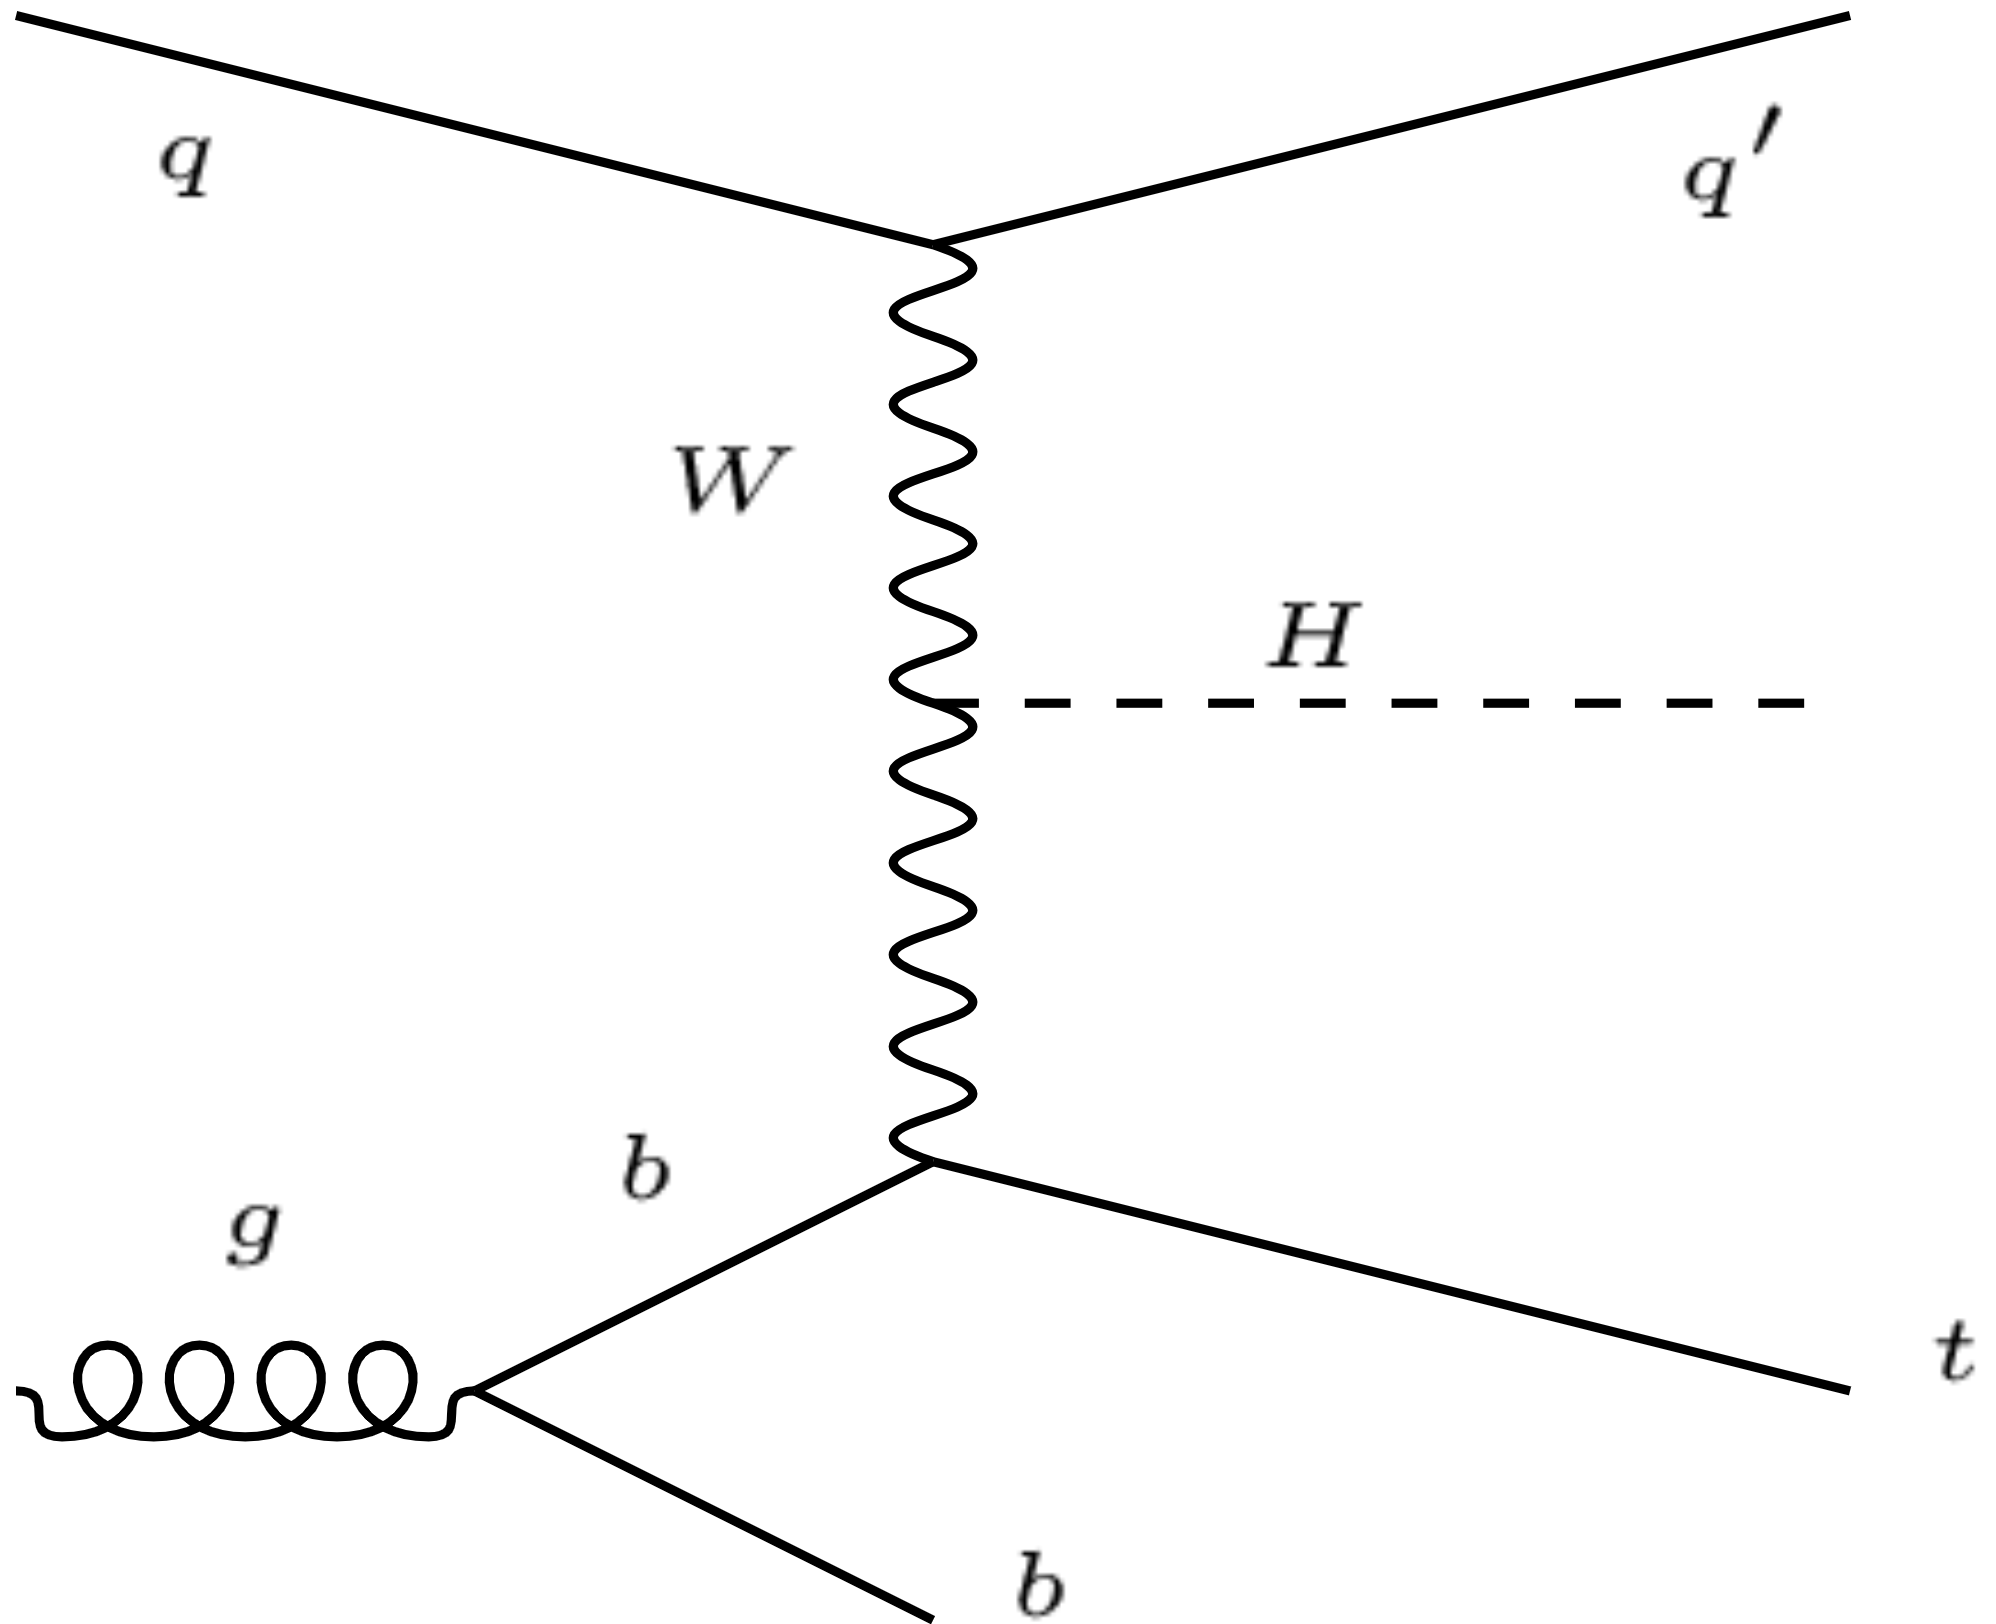
\includegraphics[width=.5\textwidth]{Feynman_diagrams/old/tChnnnael_tHq_H_from_W}
\caption{LO Feynman diagram for the \tHq process}
\label{fig:tHq:TruthFeyman:HfromW}
\end{figure}

% B-quarks
\paragraph{\Pbottom quarks}\mbox{}\\
 Afterwards the second \Pbottom quark is identified as the one whose parent
 is a gluon since it is originated from the gluon splitting. The \Pbottom originated 
 from the top decay system is saved as well. In Figure \ref{fig:tHq:pTvsEta_bQuark}
 the $\pT$ and $\eta$ distributions of these to quarks are compared using the truth-level
 inforamtion.
 
\begin{figure}[htbp!]
\centering
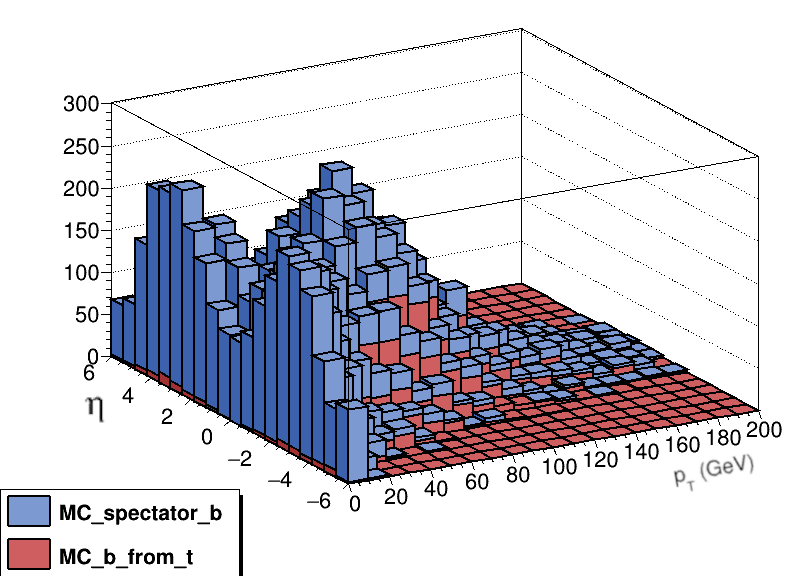
\includegraphics[width=.49\textwidth]{Chapter5_tHq/Truth_b_quark_Comb_Stack_inverted}
\includegraphics[width=.49\textwidth]{Chapter5_tHq/Truth_b_quark_Comb_Stack}

\caption{Truth-level $\pT$ vs $\eta$ distributions for the spectator (or second) \Pbottom quark and 
the \Pbottom quark produced in the top quark decay for the \tHq events. Note
how the $\pT$ of the second \Pbottom quark is smaller. This causes the spectator quark to not
pass the trigger requirements.}
\label{fig:tHq:pTvsEta_bQuark}
\end{figure}
 
\paragraph{Further decays}\mbox{}\\
Finally, all the possible decays from the Higgs children are considered.
These are further decayed several times to explore all possible final states.
The range of possible combinations is wide and a single final
state can be achieved in more than one way. 
For all \tHq events, the information of
all particles involved in the event is stored in the NTuples.

%https://gitlab.cern.ch/IFIC-Valencia/tHqIFIC/-/blob/Dileptau/tHqGraphics/thq-truth/4TruthHistos.py
 
 
\begin{comment}
% General features
\paragraph{General Features}\mbox{}\\
The variables associated to the
Higgs boson, top quark and their corresponding decay
products have the following general features:

\begin{itemize}
\item The parton-level truth variables (i.e.\ the ones starting with
  \texttt{MC\_}) are only filled properly when the Higgs
  boson decays to \WW, \ZZ or $\tau\tau$ (except the variable
  \texttt{MC\_H\_decay} which is filled for all events) and when the
  top quark decays into $Wb$.
\item For each variable, there are five branches in the
  \texttt{truth} tree. Their names are the variable name plus one of the following suffixes: \texttt{\_pt}, \texttt{\_eta}, \texttt{\_phi}, \texttt{\_m} and
  \texttt{\_pdgId}. Some of the $\tau$ related variables have the \texttt{\_isHadronic} suffix. 
\item The \texttt{\_isHadronic}-type variables refer only to $\tau$ particles
  and they store wether the $\tau$ decays hadronically or leptonically. 
  If the $\tau$ decays to a light lepton, it stores the PDG-ID of that lepton
  and if it decays hadronically it stores the PDG-ID of the \PWm for $\tau^-$ 
  and  the \PWp for $\tau^+$.
\item The default value is \(-1000\) for the branches ending with \texttt{\_pt},
  \texttt{\_eta}, \texttt{\_phi} , \texttt{\_m} while -9999 is the
  default value for the ones ending with \texttt{\_pdgId} and \texttt{\_isHadronic}. 
\item For Higgs boson decays, \texttt{\_decay1\_} stores particles with positive PDG-ID
  while \texttt{\_decay2\_} stores particles with negative PDG-ID.
\item Unless stated otherwise, we are storying the particles after the final state  radiation (FSR) \textit{i.e.} right before decaying. %Review how accurate is this
%   \item For the decay products of the $W/Z$ bosons and $\tau$'s, \texttt{\_decay1\_} is used to store either hadron or
%   lepton information (generally with negative PDF-ID) while
%   \texttt{\_decay2\_} is used for the either neutrino or the lepton information (generally with positive PDG-ID).
\end{itemize}
\end{comment}

%\paragraph{Results}\mbox{}\\
 %\pablo{Pie charts from TopPartons info}

 
 % Scripts: 
%.  https://gitlab.cern.ch/atlas/athena/-/blob/21.2/PhysicsAnalysis/TopPhys/xAOD/TopPartons/Root/CalcThqPartonHistory.cxx
%.  https://gitlab.cern.ch/atlas/athena/-/blob/21.2/PhysicsAnalysis/TopPhys/xAOD/TopPartons/Root/PartonHistoryUtils.cxx

\subsubsection{Theoretical calculation}
\label{sec:ChaptH:Sig:truth:Calculations}
%\paragraph{Calculations}\mbox{}\\
 On the other side, the theoretical calculations are used to determine the fraction of each decay channel that are present in the \dileptau. This predictions should be match the fractions obtained with \texttt{TopPartons}. I performed this 
calculations not only for the \dileptau channels but also for the $3\ell$. For the calculations the 
these Higgs-decay fractions are used:
\begin{itemize}
	\item  BR(\Htautau)$= 56.65\%$
	\item  BR(\HWW)$= 5.12\%$ 
	\item  BR(\ZZ)$= 37.43\%$
\end{itemize}
The decay products of each pair of Higgs children are combined and the total decay fractions of 
these combinations computed. To do so, the following decay ratios are used.

\begin{multicols}{2}
For the \Ptau leptons 
\begin{itemize}
	\item  BR($\tau \rightarrow \Pe \Pnu \Pnu)= 17.82\%$
	\item  BR($\tau \rightarrow \Pmu \Pnu \Pnu)= 17.39\%$
	\item  BR($\tau \rightarrow$ Hads.)$= 64.74\%$
\end{itemize}
\columnbreak
For the \PW bosons
\begin{itemize}
	\item  BR($\PW \rightarrow \Pe \Pnu) = 10.71\%$
	\item  BR($\PW \rightarrow \Pmu \Pnu) = 10.63\%$
	\item  BR($\PW \rightarrow \Ptau \Pnu) =11.38\%$
	\item  BR($\PW \rightarrow$ Hads.)$= 67.41\%$
\end{itemize}
\end{multicols}
For the \PZ bosons
\begin{itemize}
	\item  BR($\PZ \rightarrow \Pe \Pe)= 3.36\%$
	\item  BR($\PZ \rightarrow \Pmu \Pmu)= 3.36\%$
	\item  BR($\PZ \rightarrow \Ptau \Ptau)= 3.36\%$
	\item  BR($\PZ \rightarrow \Pnu \Pnu)= 20\%$
	\item  BR($\PZ \rightarrow$ Hads.)$= 69.91\%$
\end{itemize}

Note that the BRs of the considered decay modes are normalised
so that its sum is the 100\%. \pablo{citar el PDG para estos números}
If the \PW or \PZ decays to a \Ptau, it is further decayed into either
a $\emu$ or \tauhad. 
For each of the Higgs-decay modes the possible final states are studied
and its correspondent fractions calculated. 

For \Htautau:
\begin{itemize}
	\item  BR($\tautau \rightarrow \emu + \emu)= 12.41\%$
	\item  BR($\tautau \rightarrow \emu + \tauhad)= 45.63\%$
	\item  BR($\tautau \rightarrow$ Hads.)$= 41.51\%$
\end{itemize}

For \HWW the first two elements of the list take part 
in the \dileptau signature when the \tauhad comes from 
the \Ptop quark in the first item and from the \PHiggs boson
in the second. 
\begin{itemize}
	\item  BR($\WW \rightarrow \emu +\emu)= 6.42\%$ 
	\item  BR($\WW \rightarrow \emu +\tauhad)= 3.73\%$
	\item  BR($\WW \rightarrow \emu$ +Hads$)= 34.17\%$
	\item  BR($\WW \rightarrow$ Hads.)$= 55.92\%$
\end{itemize}

For the \ZZ the $\ZZ \rightarrow 2 \times \emu$ contributes 
to the \dileptau signature when the \tauhad is produced in the
\Ptop quark system. When the \Ptop quark decays into a 
light lepton, the $\ZZ \rightarrow \emu + \tauhad$ mode contributes
to the \dileptau final state.
\begin{itemize}
	\item  BR($\ZZ \rightarrow 4 \times \emu)= 0.52\%$ 
	\item  BR($\ZZ \rightarrow 2 \times \emu)= 12.85\%$
	\item  BR($\ZZ \rightarrow \emu +\tauhad)= 12.85\%$
	\item  BR($\ZZ \rightarrow 4 \times \nu$+Hads$)= 80.82\%$
	\item  BR($\ZZ \rightarrow 2 \times \tauhad)= 2.82\%$	
	\item  BR($\ZZ \rightarrow 3 \times \emu + \tauhad)= 0.22\%$
\end{itemize}


For the top-quark system only the $\Ptop \rightarrow \PW + \Pbottom$
mode is taken into account and the \PW is further decayed until there are
either hadrons, light leptons or a \tauhad. Expect when the \PW decays directly
into hadrons, all modes contribute to the \dileptau channel.


Combining all the decay modes presented brings out wide variety of final states 
with different probabilities. For the \dileptau final state, these results are summarised in
Table \ref{tab:ChaptH:TruthSummary}.% and Figure \ref{fig:tHq:Truth:PieChartHiggsDecayModes}.
Additionally, from these calculations can be deducted that from all \tHq events, only
a $3.72\%$ decay into a \dileptau final state. %  dileptau = 3.715767739%
From these, more than in 80\% of cases the \tauhad is produced in
the Higgs-boson-decay chain.

\begin{table}[h]
\centering
\begin{tabular}{l|ll|l}
\toprule
       \multicolumn{1}{c|}{Higgs decay} 	& \multicolumn{2}{c|}{Origin of \tauhad} &    \multirow{2}{*}{Total}     \\ \cline{2-3}
      \multicolumn{1}{c|}{channel}  		& Top quark        				& Higgs boson       &   \\ \midrule
\Htautau 	& 5.06      					& 64.06        		      			& 69.13	\\
\HWW    	& 9.01         				& 18.01              				& 27.02 	\\
\HZZ    	& 2.22          				& 1.64               				& 3.85   	\\ 
\midrule
Total  	& 16.29           				& 83.71              				& 100.00 	\\
\bottomrule
\end{tabular}
%	OLD RESULTS
%	\Htautau 	& 6.96    					& 88.11        		      			& 95.07  \\
%	\HWW    	& 1.41         				& 2.82              					& 4.23  \\ 
%	\HZZ    	& 0.40          				& 0.297               				& 0.70   \\ \midrule
%	Total  	& 8.78           				& 91.22              				& 100.00 \\
\caption{Contribution as percentage of each Higgs-decay channel to the \dileptau final state. Here is also presented whether the hadronic tau was generated from the top quark or the Higgs boson decay chain.}
\label{tab:ChaptH:TruthSummary}
\end{table}
% Describir los cálculos que hay aquí https://docs.google.com/spreadsheets/d/1e5kLqJrDCyxE28ecdznN4IDwZtDTQz0pQHcXfehRsYM/edit#gid=0
	

%\begin{figure}[htbp!]
%\centering
%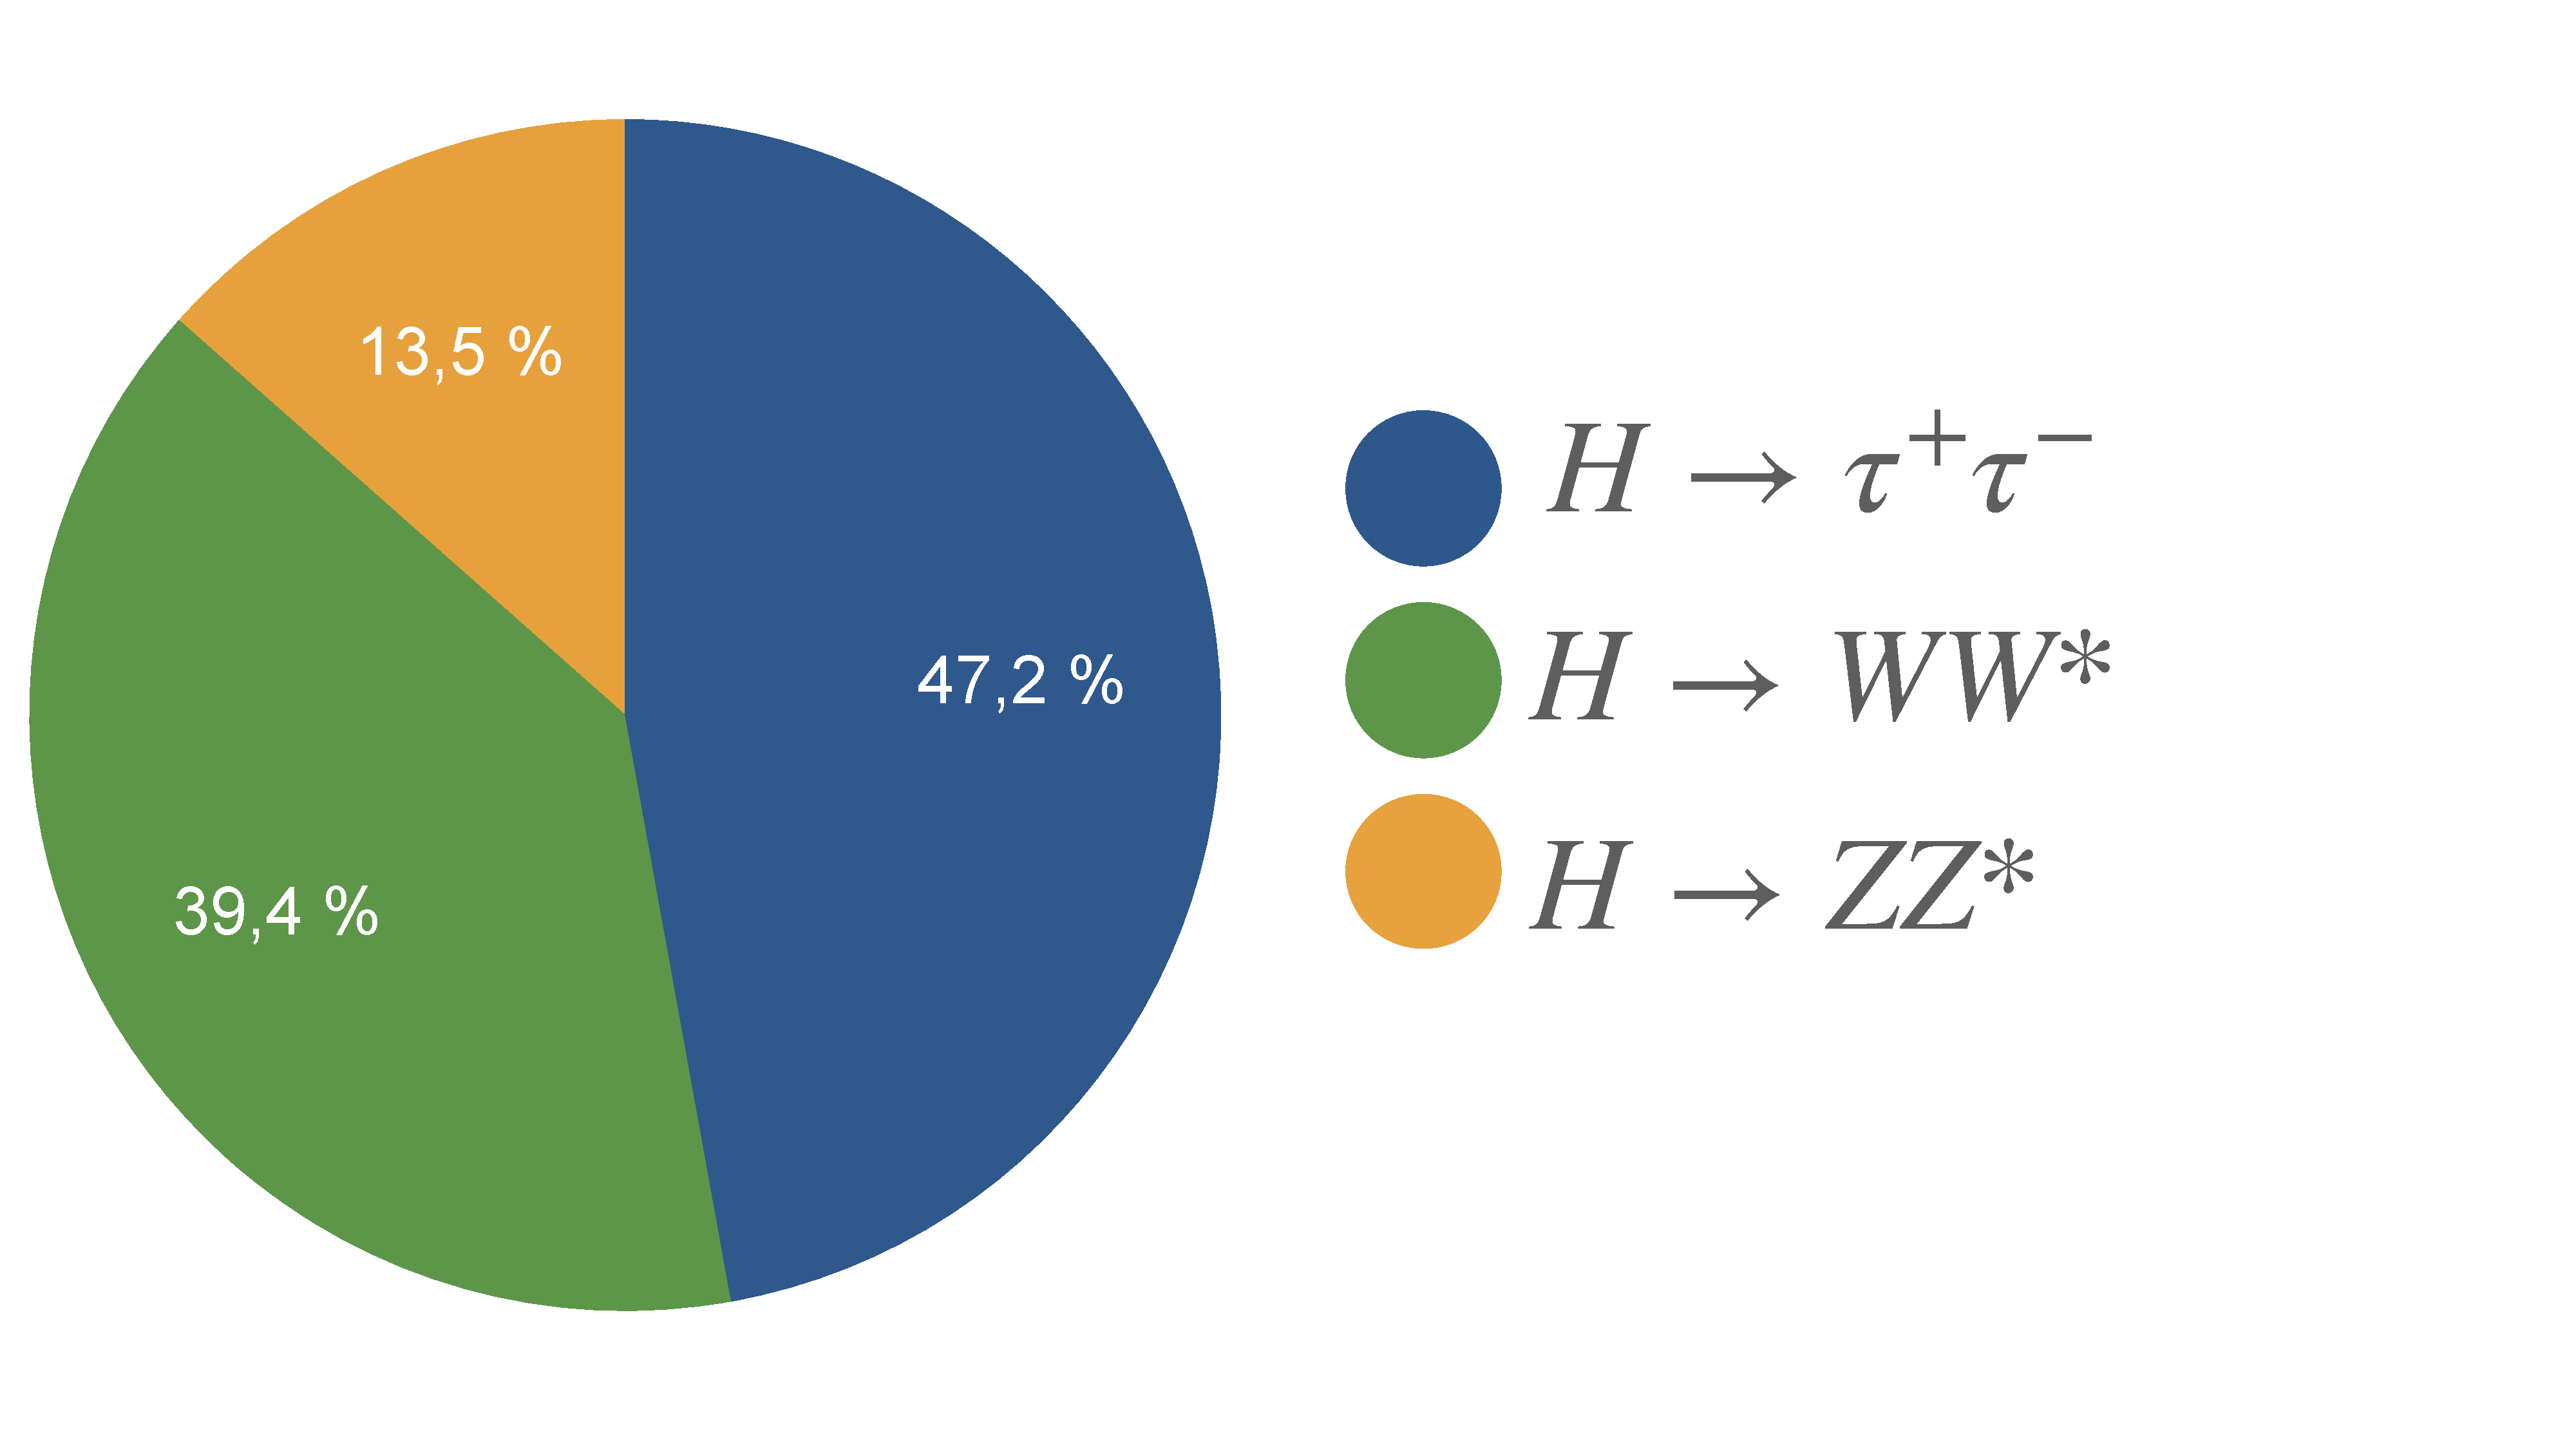
\includegraphics[width=.75\textwidth]{Chapter5_tHq/PieChartHiggsDecayModes}
%\caption{Relative contribution of each Higgs-decay channel to the \dileptau final state. Results obtained from theoretical 
%calculations. \pablo{este pie chart está mal}}
%\label{fig:tHq:Truth:PieChartHiggsDecayModes}
%\end{figure}


%> truth = generator + parton shower + hadronisation
%> The studies I did were done at generator level
%> Particle level is part of truth information
%> Detector level = reconstruction level + calibration + 

%source: https://docs.google.com/spreadsheets/d/1e5kLqJrDCyxE28ecdznN4IDwZtDTQz0pQHcXfehRsYM/edit#gid=0

\subsubsection{Comparison between software and calculation results}
The last step to validate the code developed for the truth
is to contrast the output of \texttt{TopPartons} to the theoretical calculations and check that
both are in agreement.
The metric used to perform the comparison is the ratio between the \tHq(\dileptau) event yields
 in a particular Higgs-decay channel and all the events in that particular decay mode:  

\begin{equation*}
    \frac{\text{Events}(H \rightarrow \text{Decay channel} \rightarrow  \dileptau)}{\text{Events}(H \rightarrow \text{Decay channel)}}\, .
\end{equation*}

In Table \ref{tab:ChaptH:Prediction_VS_TopPartons}, the theory-based calculations
performed in Section \ref{sec:ChaptH:Sig:truth:Calculations} are put alongside 
the results of the parton-level truth informations described in Section \ref{sec:ChaptH:Sig:truth:TopPartons}.
As can be seen, the agreement between the calculations and the \texttt{TopPartons} output agrees for
the two main Higgs-decay channels. For these, the disagreement is of 1.2\% for the $\Ptau\Ptau$  and 
5.9\% for the $\PW \PW$. In contrast, a discrepancy of 60\% is found in the $\PZ \PZ$ decay mode. 
Even though the conflict in $\PZ \PZ$ is much larger than for the other channels, this is not so problematic
since the \HZZ accounts for a very small part of the total \tHq events. 

\begin{table}[]
\centering
\begin{tabular}{l|l|l}
\toprule
Yields ratio								&   Calculation   	& \texttt{TopPartons} result \\
\midrule
$\frac{\Htautau \rightarrow \dileptau }{\Htautau}$  	&   0.1246         	&  $0.1232  \pm 0.0057$ 	\\ 
$\frac{\HWW 	\rightarrow \dileptau}{\HWW}$       	&   0.0141        		&  $0.0151  \pm 0.0009$   \\ 
$\frac{\HZZ 	\rightarrow \dileptau }{\HZZ}$           	&   0.0164         	&  $0.0100  \pm 0.002$     \\ \bottomrule
% \textbf{$3l$}                & \textbf{Prediction} & \textbf{Result} \\ \hline
%$H \rightarrow WW \rightarrow SR(3l) / H \rightarrow WW$                &   0.0162         &  $0.0169  \pm 0.0010$      \\ \hline
%$H \rightarrow \tau \tau \rightarrow SR(3l) / H \rightarrow \tau \tau$  &   0.0314         &  $0.0271  \pm 0.0027$     \\ \hline
%$H \rightarrow ZZ \rightarrow SR(3l) / H \rightarrow ZZ$                &   0.0325         &  $0.0152  \pm 0.0031$      \\ \hline
\end{tabular}
\caption{Theoretical predictions compared to the \texttt{TopPartons} output. 
The uncertainty on the second column corresponds to the statistical error. }
% both the count and errors are computed with  the event weights.
\label{tab:ChaptH:Prediction_VS_TopPartons}
\end{table}

%\FloatBarrier 


%%%%%%%%%%%%%%%%%%%%%%%%%%%%
%           Lepton-origin assignment     %
%%%%%%%%%%%%%%%%%%%%%%%%%%%%
\subsection{Light-flavoured-lepton origin assignment}
\label{sec:ChaptH:Sig:LepAsign}
% Importance
The two light leptons in the final state of the \dileptau channel can originate either from the 
Higgs boson or the top quark. The ambiguities regarding the origin of these light-flavoured
leptons, make the reconstruction of the top quark and Higgs boson systems extremely difficult.
Nevertheless, the electric charge of these leptons could provide us useful information to probe their origins.

To have knowledge of whether the light-flavoured leptons in the final state are originated from
the Higgs boson or the top quark is very beneficial in order to both reconstruct the event and
design variables at reconstruction level with high discriminant power. As is show in 
Sections \ref{sec:ChaptH:EventSelection:SR} and \ref{sec:ChaptH:EventSelection:CR},
the variables using the lepton assignment information play a relevant role not only in 
the definition of the signal-enriched section but also the in the determination of 
 the control regions to constrain the most important background processes.

According to the calculations performed by combining the BR of the Higgs boson, the top quark 
and all its decay products (see Section \ref{sec:ChaptH:Sig:truth}),
in the \dileptau channel of \tHq production, the \tauhad is produced 83.7\% of times as a 
product of the Higgs-boson decay in opposition to the 16\% in which it comes from the top-quark
disintegration. 

\paragraph{Origin association for \dilepOStau}\mbox{}\\ %opposite-sign leptons
In the dominant scenario (\tauhad from Higgs) the association of which light-flavoured
lepton comes from the top-quark decay and which one comes from the Higgs-boson decay can be
done directly if these two leptons have opposite electric charge, i.e. in the \dilepOStau channel.
Since in Higgs boson is neutrally charged, the sum of the charge of its decay products should be zero. Therefore,
in the OS channel, while the light lepton with opposite charge to that of the \tauhad is the one coming
from the Higgs, the other lepton, i.e. the one with the same charge as \tauhad, is the one originated 
from the top-quark decay.



\paragraph{Origin association for \dilepSStau}\mbox{}\\ %same-sign leptons
In contrast to the \dilepOStau channel, in the case of \tauhad from Higgs,
 when the two light leptons have the same electric charge, \dilepSStau,
it is not possible to know, a priori, which of the leptons comes from the top-quark system and which 
from the Higgs-boson decay. 
%All of this, assuming that the \tauhad comes from the Higgs boson, otherwise,
%if the \tauhad was produced as a decay product from the top, it would not make sense 
%to talk about the lepton origin since both light leptons would be associated to the Higgs system.

In order to perform this association for the \dilepSStau three methods %relying in the truth-level information
have been tested. These are: %\pablo{Igual no vale la pena mencionar los otros porque tampoco se entienden bien}
\begin{itemize}
	\item \textbf{NN approach}:  A neural network based on the Keras framework 
	was trained to perform the assignment task. In labeling the data, it was assumed 
	that the l$\ell_{1}$ always originates from the top quark. Truth-level studies have 
	shown that in most cases, the lepton coming from the decay chain of the top quark 
	is the leading lepton. This is because the top quark typically carries more momentum 
	than the Higgs boson. However, it should be noted that this assumption is only correct 
	61.1\% of the times. Therefore, using a machine learning method trained with a label 
	of such low quality is not considered reliable and, hence, this approach is discarded. 
	
	%\pablo{Esta es la NN que desarrolló Cyrus y, la verdad, 
	%es que no servía para nada. Quizás no valga la pena ni dedicarle un párrafo.}
	% Developed by "Walther, Cyrus Pan" 
	% source: http://cds.cern.ch/record/2743809/files/Summer_Student_Report_Cyrus_Walther.pdf
	
	\item \textbf{Cut-based classification}: The most straightforward method to carry 
	out the lepton assignment involves employing variables capable of distinguishing 
	the origin of the lepton in the \dilepOStau scenario, where the origin is known. 
	Then, some criteria is applied over these variables to define an algorithm to
	assign the lepton origin. The visible Higgs mass (\Hvismass) and the reconstructed 
	top mass (\toprecomass) are used for this purpose and the logic is the following:
	
	\resizebox{0.9\textwidth}{!}{\begin{tabular}{ll}
 		If $\Delta(m_{viss}^{\PHiggs}) > 57\,$GeV: & Assign lepton to top quark for which \(\Hvismass(\leptop) > \Hvismass(\lepH)\) \\
		%$m_{viss}^{\PHiggs}(\leptop) > m_{viss}^{\PHiggs}(\Pl_{\text{H}})$ \\
  		If $\Delta(m_{viss}^{\PHiggs}) < 57\,$GeV: & Assign lepton to top quark for which \(\toprecomass(\leptop) > \toprecomass(\lepH)\) \\
		%$m_{reco}^{top}(\leptop) > m_{reco}^{top}(\Pl_{\text{top}})$ \\
	\end{tabular}}
	where $\Delta(m_{viss}^{\PHiggs}) = \Hvismass(\ell_{1}) - \Hvismass(\ell_{2})$. 
	This algorithm provides and accuracy of about 80\% when evaluated on the
	\dilepOStau sample exclusively .

	
	\item \textbf{BDT-based method}: To accurately assign the origin of the light lepton 
	in the \dilepSStau scenario, a gradient BDT method was developed. The BDT is 
	implemented using the TMVA library of ROOT, whose technicalities are discussed 
	in Appendix \ref{chap:Appendix:BDT}.
	
	This BDT-based method uses labels derived from the truth-level information and is 
	trained using reconstruction-level variables. Subsequently, it can later predict the 
	lepton origin for unlabelled data.  The methodology employed in this approach is
	 thoroughly described in this section, covering the creation of the labels, the training 
	 process, and the application of the BDT model.
	%\footnote{A BDT is a type of machine learning algorithm used for 
	%both regression and classification tasks.The details of how a BDT work 
	%are discussed with detail in Appendix \ref{chap:Appendix:BDT}. } 

\end{itemize}

Among the three developed methods, the BDT-based approach demonstrates 
superior results. The implementation of the BDT-based approach can be outlined 
through the following procedural steps:

\begin{enumerate}
	\item \textbf{Labelling}: The creation of a label for supervised training through the use of truth-level 
		information and the establishment of categories for classification. In 
		Section \ref{sec:tHq:origin:LeptonAssignment_truth_reco_DeltaRCone}
		this is discussed and the categories ``Type$\,$1'' and ``Type$\,$2'' are defined.
		
	\item \textbf{Feature importance}: The selection of reconstruction-level 
		input features with discriminatory capacity between the Type$\,$1 
		and Type$\,$2. These variables cannot be later on used in the region-definition BDT. 
		Section \ref{sec:ChaptH:Sig:LepAsign:SS:BDT:inputFeatues} discusses the set of variables used.
		
	\item \textbf{Hyperparameter optimisation}: The optimisation of the training 
		hyperparameters, which is described 
		in Section \ref{sec:ChaptH:Sig:LepAsign:SS:BDT:hyperparameters}.
	
	\item \textbf{Negative weight usage}: The choice of the negative-weights-treatment strategy. 
		This matter is discussed 
		in Section \ref{sec:ChaptH:Sig:LepAsign:SS:BDT:NegWeights} and complemented
		by Appendix \ref{chap:Appendix:NegWeights}.
	
	\item \textbf{Training}: The supervised training of the model to classify events according
		to the origin of the light lepton is shown in 
		Section \ref{sec:ChaptH:Sig:LepAsign:SS:BDT:Training}.

	\item \textbf{Injection}: The application of scores and search 
		of the optimal classification threshold. This last step
		is presented in Section \ref{sec:ChaptH:Sig:LepAsign:SS:BDT:Application}.
\end{enumerate}


%%%%%%%%%%%%%%%%%%%%%%%
%           Label with truth-reco matching        %
%%%%%%%%%%%%%%%%%%%%%%%
\subsubsection{Labelling the \dilepSStau with the reconstruction-level and truth-level matching}
\label{sec:tHq:origin:LeptonAssignment_truth_reco_DeltaRCone}
Even though at reconstruction level it is not known which are the parents of the particles in the final
state, at parton level\footnote{The definitions of truth, parton and reconstruction levels are given in
Section \ref{sec:Chap3.1:MC}.} this informations is accesible, in other words, the origin\footnote{By origin of a 
light lepton is meant whether this particle comes from the Higgs-boson-decay chain or the top-quark-decay chain.}
 of the light leptons is known.
For a given event, it is possible to access to both the particle-level and parton-level information simultaneously.
Having the parton-level leptons, whose parents are known, and the reconstruction-level leptons, whose parents
need to be identified, it is possible to compare them to create an association. Specifically, identify which 
parton-level lepton correspond to which reconstructed lepton.
The aim of this relation is to assign the leading ($\Pl_{1}$) and sub-leading ($\Pl_{2}$) light leptons at reconstruction level to the
the ``lepton from top-quark-decay chain'' ($\Pl_{\text{top}}$) and ``lepton from Higgs-boson-decay chain'' ($\Pl_{\text{Higgs}}$) 
at truth level. 

In order to vinculate the reconstruction-level light leptons to the parton-level light leptons, a \(\dR < 0.01\) cone around
each of the reconstructed leptons is built. When inside that cone there is exactly one truth-level light lepton,
there is what is called ``a match''. Figure \ref{fig:chap:tH:LepAssign:Match} presents the possibles scenarios
of the association. In order to identify properly determine the lepton origin in an event, it is required that both leptons
at reconstruction level have a match. There are two different cases for this.
The first situation is that in which the leading-light lepton is $\Pl_{\text{top}}$ and the sub-leading is $\Pl_{\text{tHiggs}}$. For the 
sake of simplicity, this configuration is named ``Type$\,$1'' and it is represented in Figure \ref{fig:chap:tH:LepAssign:Match:Type1}.
The second double-matching combination is the other way around, the leading-light lepton is $\Pl_{\text{Higgs}}$ and the sub-leading 
is $\Pl_{\text{top}}$. Pictured in Figure \ref{fig:chap:tH:LepAssign:Match:Type2}, this type of events are called ``Type$\,$2''.
On the contrary, if only one of the two reconstructed light leptons is matched (Figure \ref{fig:chap:tH:LepAssign:Match:1Match}),
none of the leptons are classified. If a less strict criteria was used, it would be possible requiere that only one of the two leptons
matches in order to classify the event (the unmatched reconstruction-level lepton would be assigned to the unmatched parton-level
lepton). The problem of the lax strategy is that while in cases like that on Figure \ref{fig:chap:tH:LepAssign:Match:1Match} it seems
clear that unmatched parton correspond to the unmatched reconstructed lepton, for events such as the illustrated in
Figure \ref{fig:chap:tH:LepAssign:Match:1Match_b} the unmatched particle does not necessarily belong to the $\Pl_{2}$ cone.
For this reason, it is mandatory that both reconstructed light leptons have a match.
Finally, in the scenario in which none of the parton-level leptons fall into the cones (Figure \ref{fig:chap:tH:LepAssign:Match:0Matchs}), 
no assignation takes place. 



\begin{figure}
\centering
\begin{subfigure}{.49\textwidth}
  \centering
  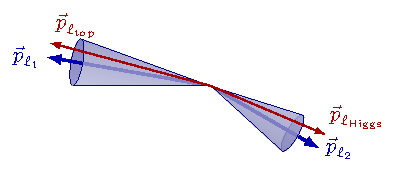
\includegraphics[width=\linewidth]{Chapter5_tHq/LeptAssociation/LepAssignement_2Matches_Type1}
  \caption{Two matches. Type$\,$1 event}
  \label{fig:chap:tH:LepAssign:Match:Type1}
\end{subfigure} 
\begin{subfigure}{.49\textwidth}
  \centering
  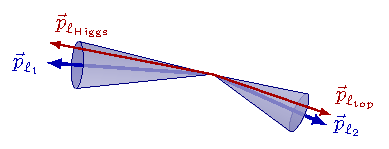
\includegraphics[width=\linewidth]{Chapter5_tHq/LeptAssociation/LepAssignement_2Matches_Type2}
  \caption{Two matches. Type$\,$2 event}
  \label{fig:chap:tH:LepAssign:Match:Type2}
\end{subfigure}

\begin{subfigure}{.49\textwidth}
  \centering
  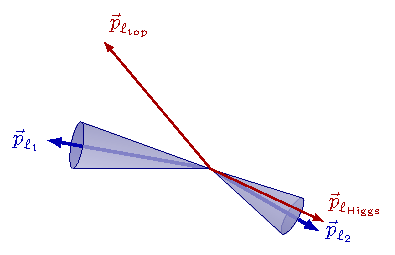
\includegraphics[width=\linewidth]{Chapter5_tHq/LeptAssociation/LepAssignement_1Match_Higgs_subleading}
  \caption{One match.}
  \label{fig:chap:tH:LepAssign:Match:1Match}
\end{subfigure}\hfill
\begin{subfigure}{.49\textwidth}
  \centering
  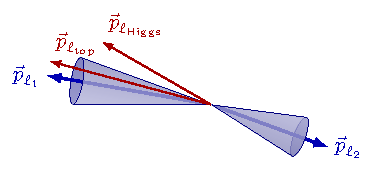
\includegraphics[width=\linewidth]{Chapter5_tHq/LeptAssociation/LepAssignement_1Match_Higgs_leading_b}
  \caption{One match.}
  \label{fig:chap:tH:LepAssign:Match:1Match_b}
\end{subfigure}

\begin{subfigure}{.5\textwidth}
  \centering
  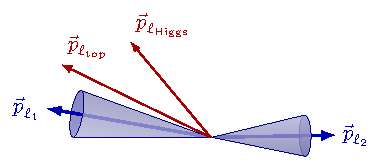
\includegraphics[width=.99\linewidth]{Chapter5_tHq/LeptAssociation/LepAssignement_0Matches_b}
  \caption{No matches}
  \label{fig:chap:tH:LepAssign:Match:0Matchs}
\end{subfigure}
\caption{	Different scenarios for the association between reconstruction-level (blue arrow) 
		and parton-level (red arrow ) light leptons. 
		Note that the labels $\Pl_{\text{top}}$ and $\Pl_{\text{Higgs}}$ are only available 
		for the parton-level particles. The labelling of the events is performed only for the 
		cases in (a) and (b) and saved in the variable \texttt{isLep1fromTop}.}
\label{fig:chap:tH:LepAssign:Match}
\end{figure}
%For this draw the https://tikz.net/jet_top/ package on latex has been used

To perform this labelling, it has been required that the \tauhad is originated in from the Higgs-boson 
system. This is imposed in order to guarantee that there are both a $\Pl_{\text{top}}$ and a $\Pl_{\text{Higgs}}$. 
The Higgs-decay channels used for these studies are the \Htautau (one $\Ptau$ decaying letonically 
and the other hadronicallly) and the \HWW. The \HZZ channel has not been included since its impact 
in the on the \dileptau production when the \tauhad comes from the Higgs is negligible. If the \tauhad is
originated in the Higgs system, only a 2.0\% of the events correspond to the \HZZ decay channel, 
contrasting with the 76.5\% of the \Htautau and the 21.5\% of the \HWW. These numbers are
presented in Table \ref{tab:chap:tH:LepAssign:FractionInSS}.

\begin{table}[]
\centering
\begin{tabular}{l|l}
\toprule
Channel 	& Fraction (\%)   \\ \midrule
\Htautau 	& 76.52 \\
\HWW     	& 21.52 \\
\HZZ   	& 1.956 \\ \bottomrule
\end{tabular}
\caption{Contribution of each Higgs-decay channel to the \dileptau final state when
demanding that the \tauhad is originated from the Higgs-boson-decay chain.
The numbers in this table are calculated from the rightmost column 
of Table \ref{tab:ChaptH:TruthSummary}.}
\label{tab:chap:tH:LepAssign:FractionInSS}
\end{table}


Following the application of criteria related to the multiplicity of \bjets, electrons, and muons, 
as well as the requirement that the Higgs boson decays to \Htautau or \HWW, the matching 
condition is imposed to set the label. This condition demands a minimum distance between
each of the reconstructed leptons to its correspondet truth lepton, $\Delta R^{\ell_{1}, \ell_{2}}_{min}$.
As each condition is sequentially applied, a reduced number of events satisfy the imposed filters. 
The corresponding entry counts at each step are summarised in
Table \ref{tab:chap:tH:LepAssign:LabellingFrac}. Note that the numbers are not the event yields 
but the entries, i.e. MC events without weight. More information about event weights is given in 
Appendix \ref{chap:Appendix:NegWeights}.

\begin{table}[]
\centering
\begin{tabular}{l|l}
\toprule
Stage				&  Entries \\ \midrule
Total \tHq sample                               & 47158 \\
Preselection: $2\emu$, $1 \Ptau$, at least $1 \bjet$ & 30113 \\
Truth selection: \tHq, $\PHiggs \rightarrow \taulep\tauhad/\PWplus\PWminus$ , $\PW \rightarrow \Pe / \Pmu / \taulep$ & 15446 \\
$\Delta R^{\ell_{1}, \ell_{2}}_{min} < 0.01$                                   & 15157 \\ \bottomrule
\end{tabular}
\caption{Unweighted events at each step of the labelling 
process. 
%Unweighted means that, when counting the 
%events, each entry is taken as one rather than taking into account the event 
%weight. More information about event weights is given in 
%Appendix \ref{chap:Appendix:NegWeights}.
The first row corresponds to the entire sample of just \tHq events. 
The second row applies a requirement on the multiplicity of final state objects.
The last row demands that the cone $\Delta R^{\ell_{1}, \ell_{2}}_{min}$ is
within 0.01, where 
$\Delta R^{\ell_{1}, \ell_{2}}_{min} = \text{min}\left(\Delta R(\protect\overrightarrow{p}_{\ell_{1}, \ell_{2}}, \protect\overrightarrow{p}_{\ell_{\text{Top}}}),\Delta R(\protect\overrightarrow{p}_{\ell_{1}, \ell_{2}}, \protect\overrightarrow{p}_{\ell_{\text{Higgs}}}) \right)$. 
} %Being $\protect\overrightarrow{p}_{\ell}$ the momentum of the lepton.
\label{tab:chap:tH:LepAssign:LabellingFrac}
\end{table}

\pablo{Should add the fraction of events that are labeled from a) the total \dileptau sample and b) from the total \dilepSStau .}
 
 
%%%%%%%%%%%%%%%%%
%           Input variables     	 %
%%%%%%%%%%%%%%%%%
\subsubsection{BDT input features}
\label{sec:ChaptH:Sig:LepAsign:SS:BDT:inputFeatues}
The choice of input variables for training a BDT is a crucial factor for achieving a good classification accuracy.
The chosen variables must exhibit the ability to effectively differentiate between Type$\,$1 and Type$\,$2. 
Figure \ref{fig:dileptau:Assignment_appendix:InputVars} displays the distributions 
of the nine chosen variables, showcasing distinct shapes for both Type 1 (blue) 
and Type 2 (red) distributions. This divergence in shapes indicates the efficacy of
these variables for classifying.

\begin{figure}[htbp!]
\centering
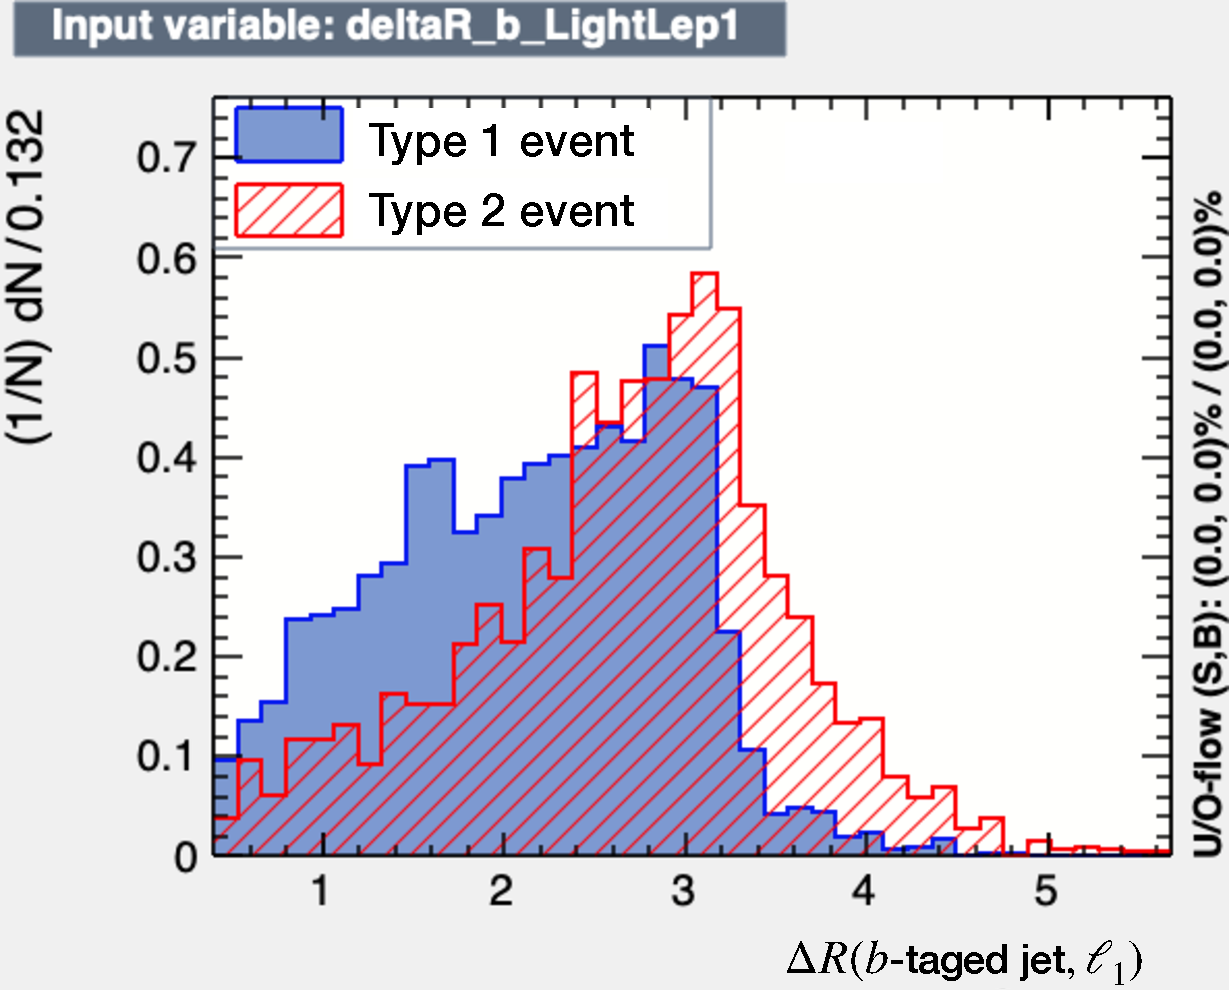
\includegraphics[width=.31\textwidth]{Chapter5_tHq/LeptAssociation/BDT_InputVariables/pdf_input_deltaR_b_LightLep1}\quad
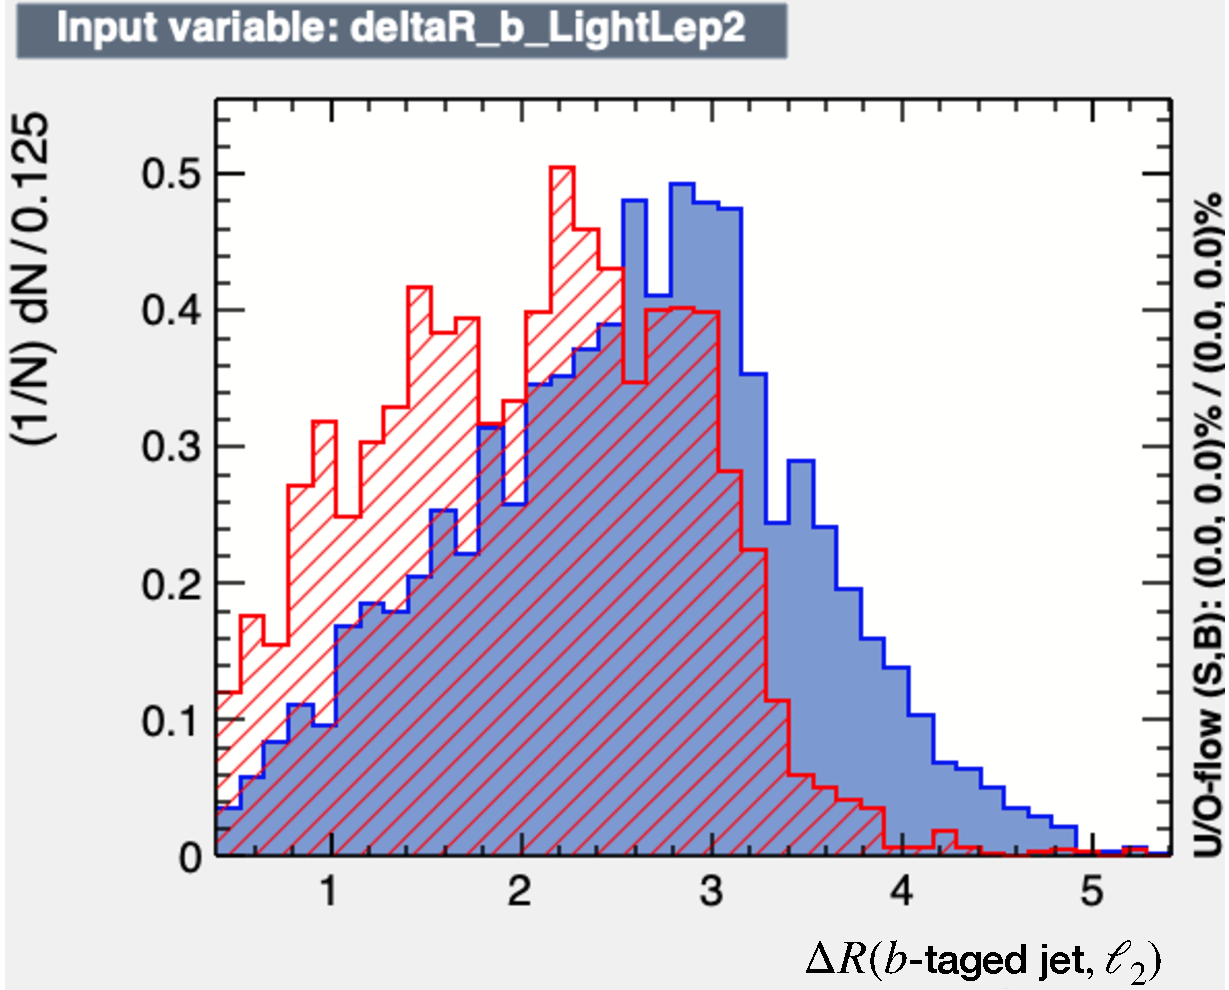
\includegraphics[width=.31\textwidth]{Chapter5_tHq/LeptAssociation/BDT_InputVariables/pdf_input_deltaR_b_LightLep2}\quad
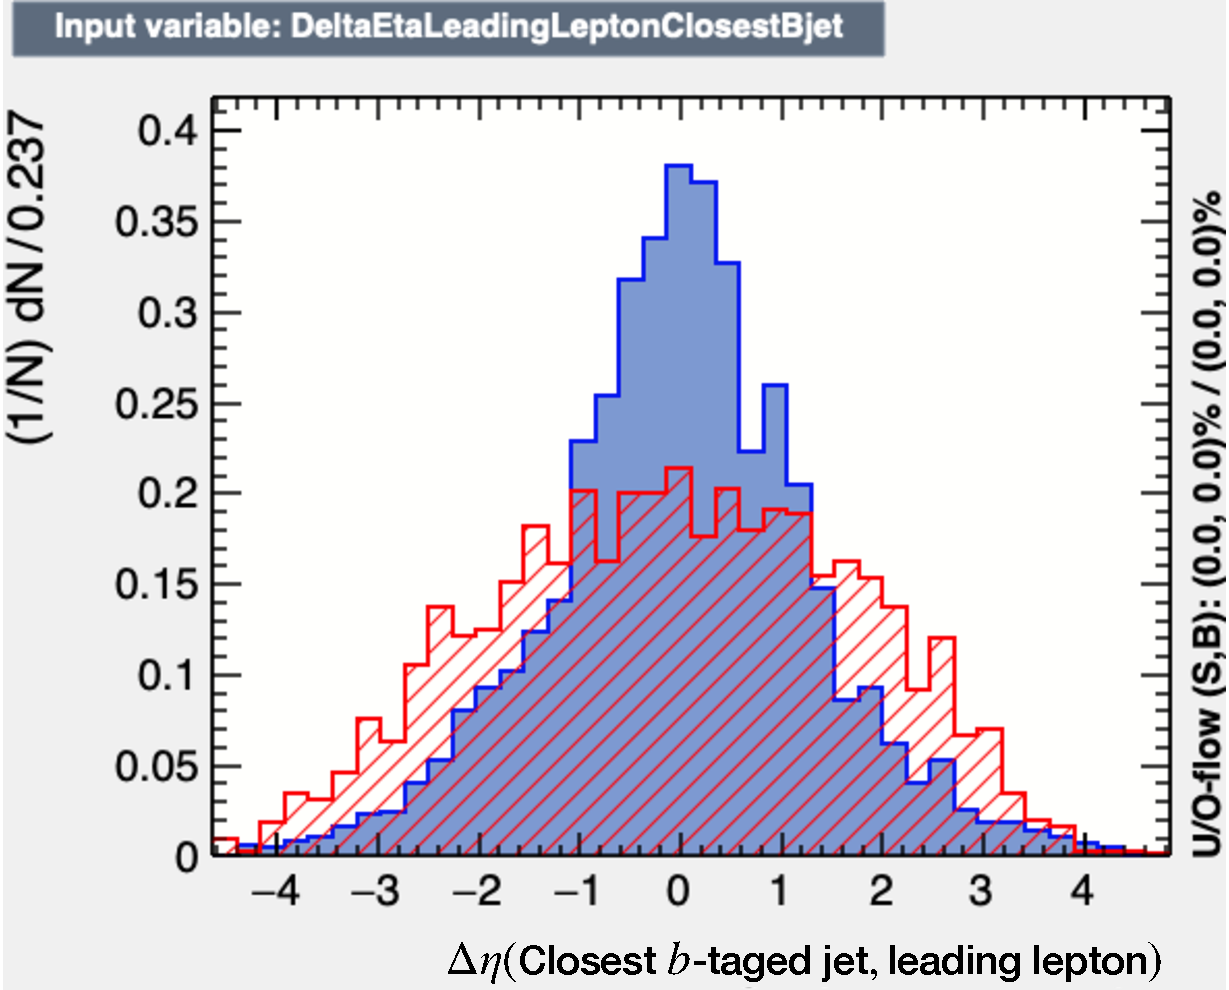
\includegraphics[width=.31\textwidth]{Chapter5_tHq/LeptAssociation/BDT_InputVariables/pdf_input_DeltaEtaLeadingLeptonClosestBjet}

\medskip
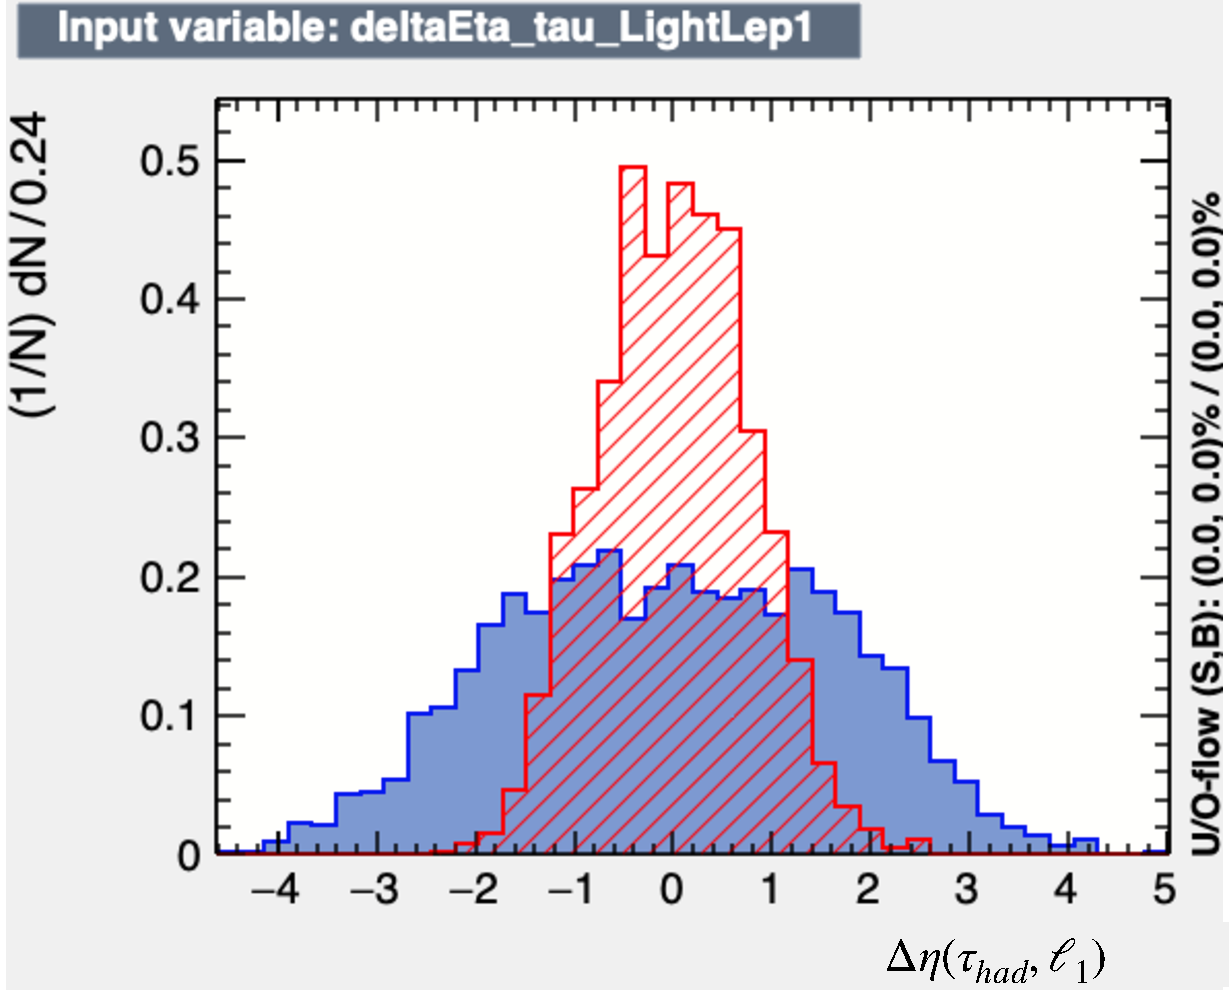
\includegraphics[width=.31\textwidth]{Chapter5_tHq/LeptAssociation/BDT_InputVariables/pdf_input_deltaEta_tau_LightLep1}\quad
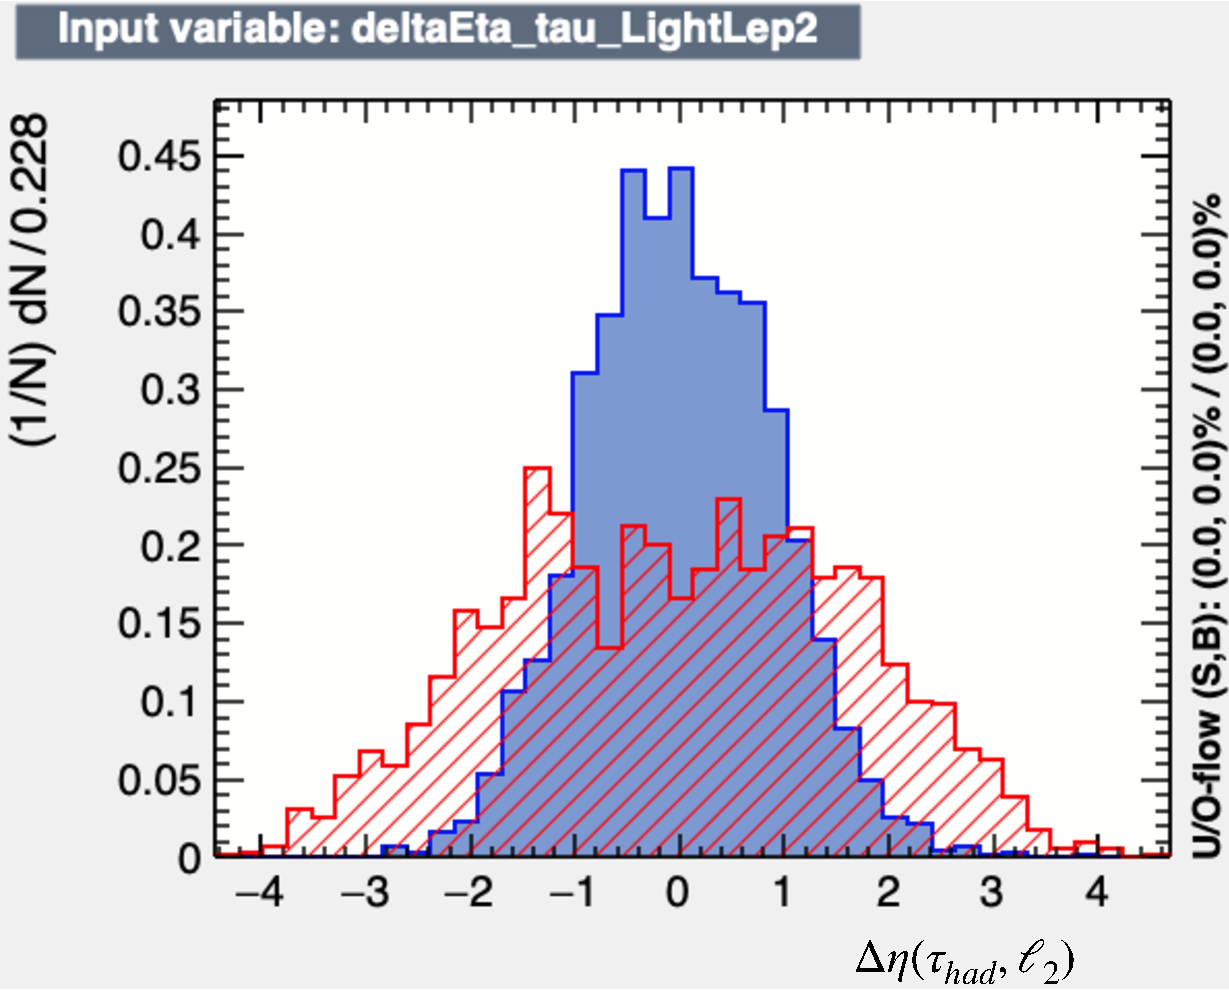
\includegraphics[width=.31\textwidth]{Chapter5_tHq/LeptAssociation/BDT_InputVariables/pdf_input_deltaEta_tau_LightLep2}\quad
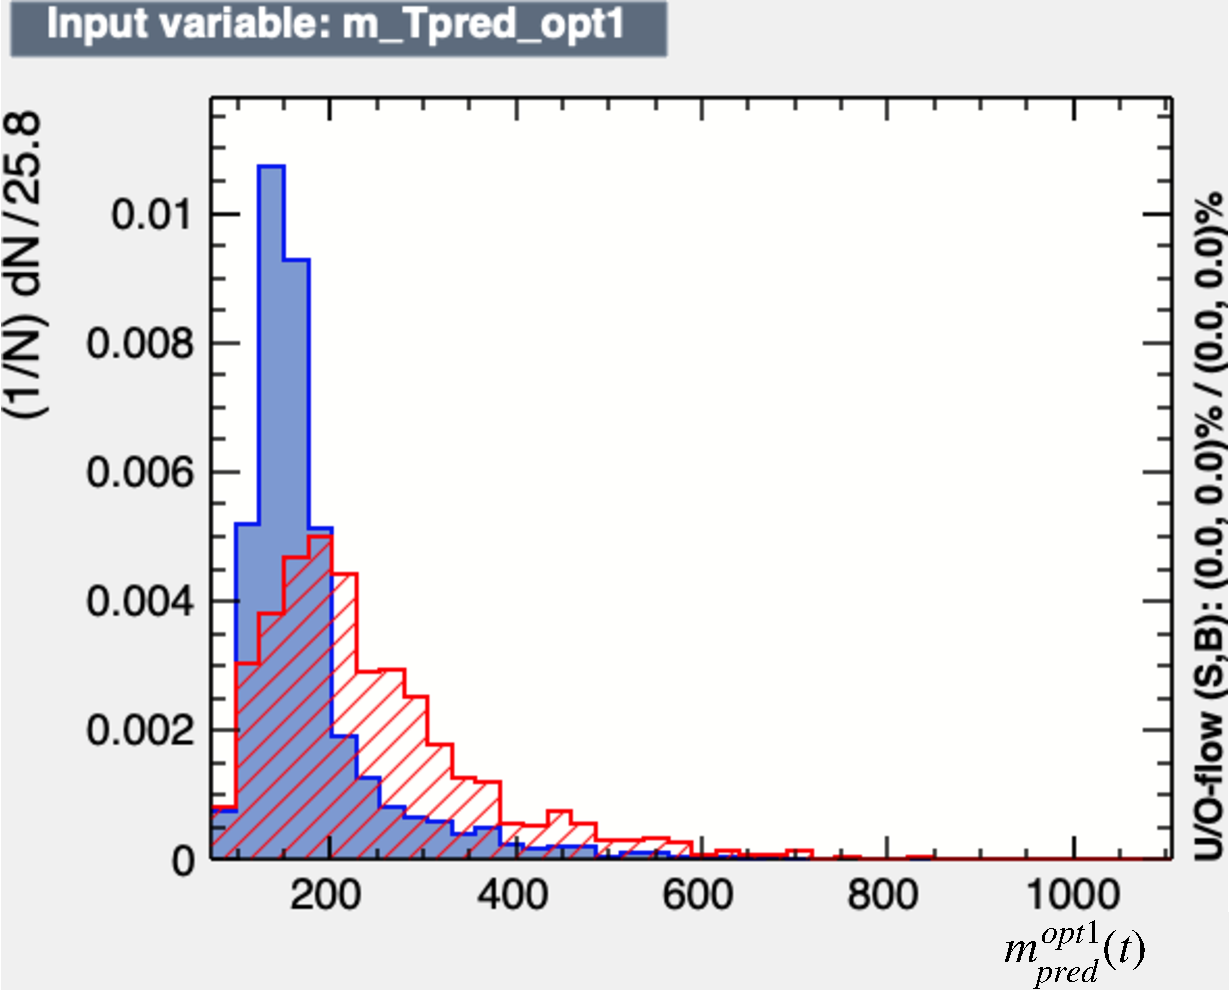
\includegraphics[width=.31\textwidth]{Chapter5_tHq/LeptAssociation/BDT_InputVariables/pdf_input_m_Tpred_opt1}
\medskip
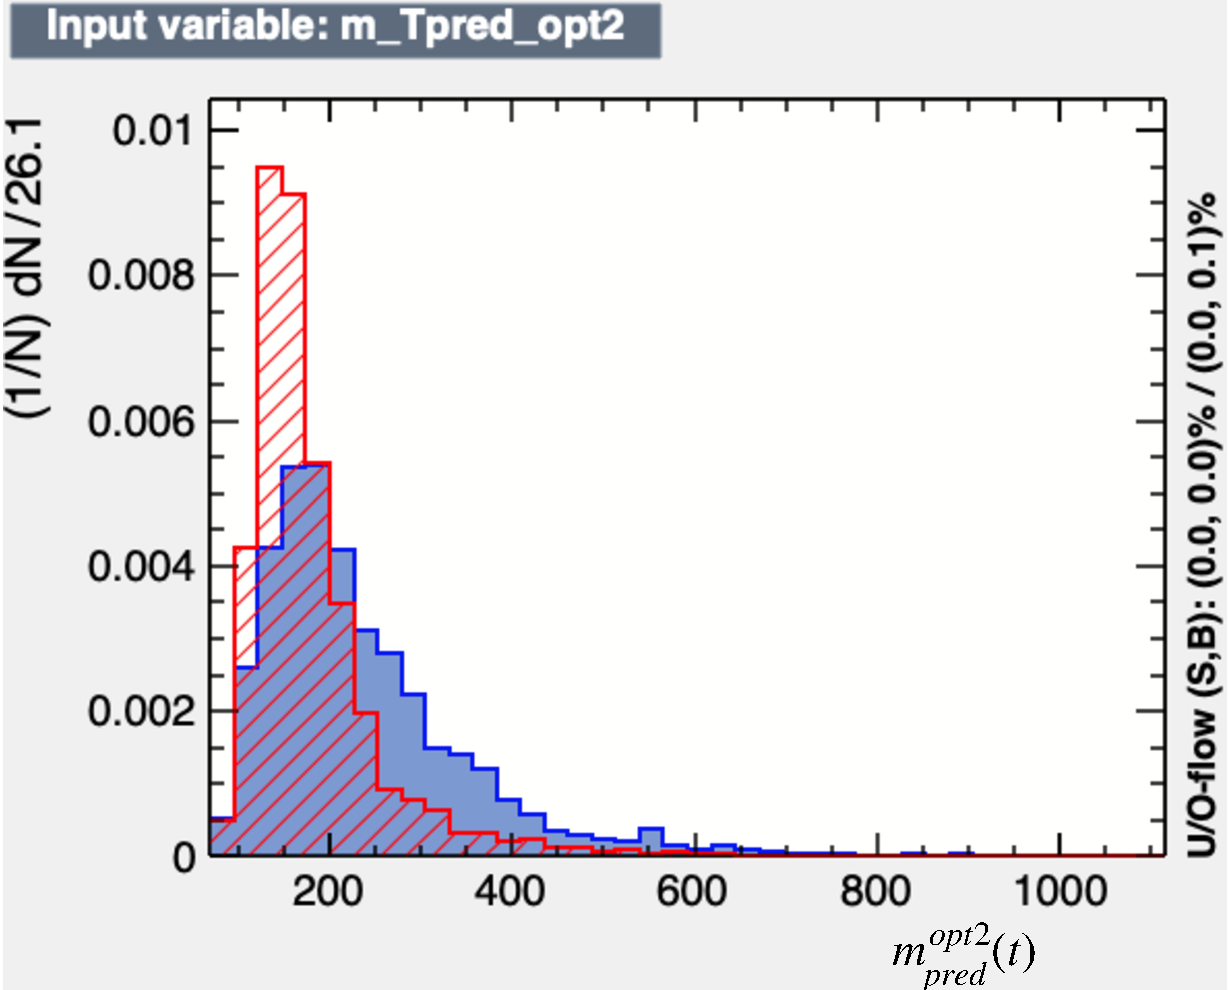
\includegraphics[width=.31\textwidth]{Chapter5_tHq/LeptAssociation/BDT_InputVariables/pdf_input_m_Tpred_opt2}\quad
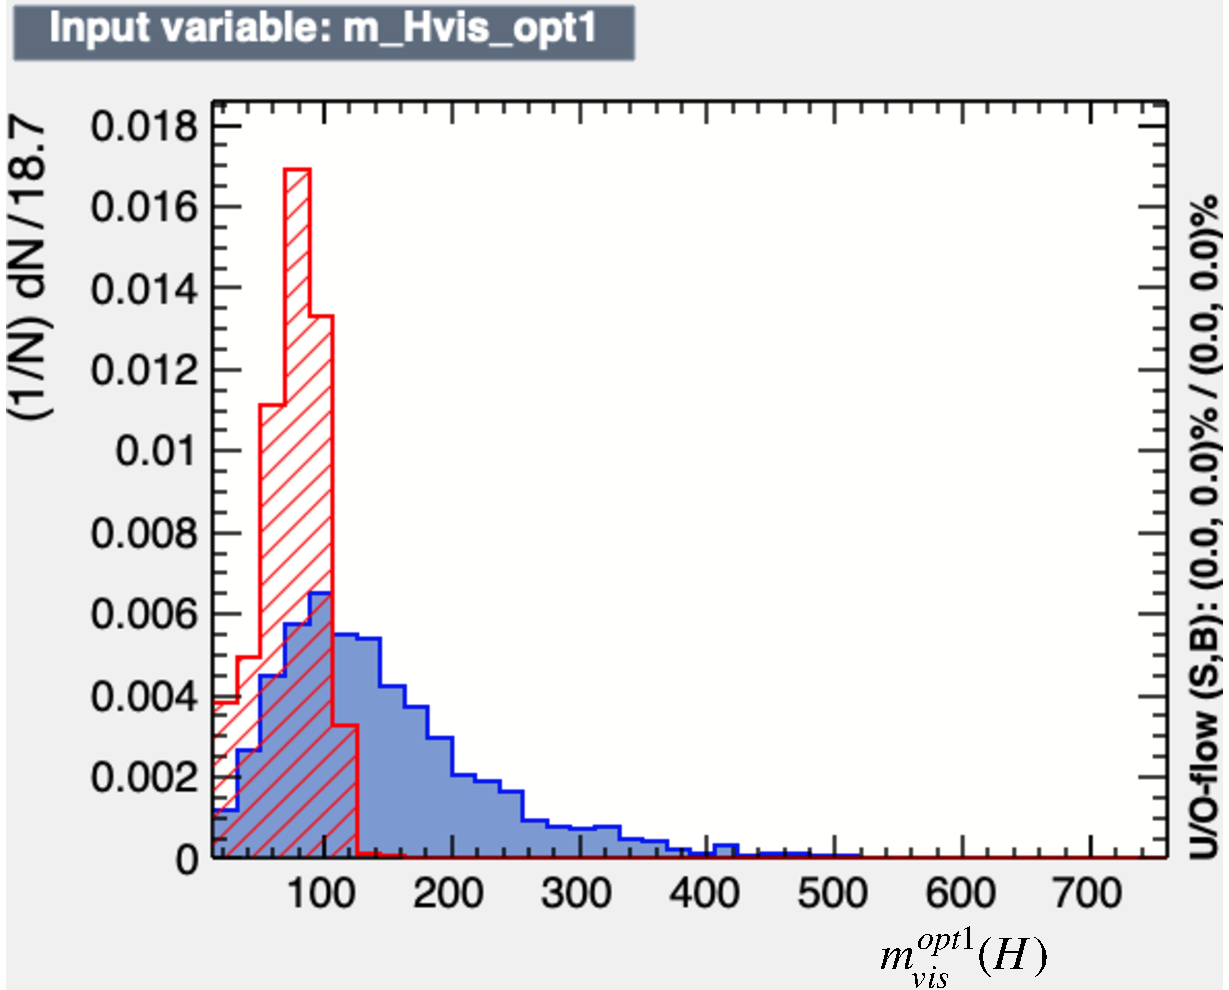
\includegraphics[width=.31\textwidth]{Chapter5_tHq/LeptAssociation/BDT_InputVariables/pdf_input_m_Hvis_opt1}\quad
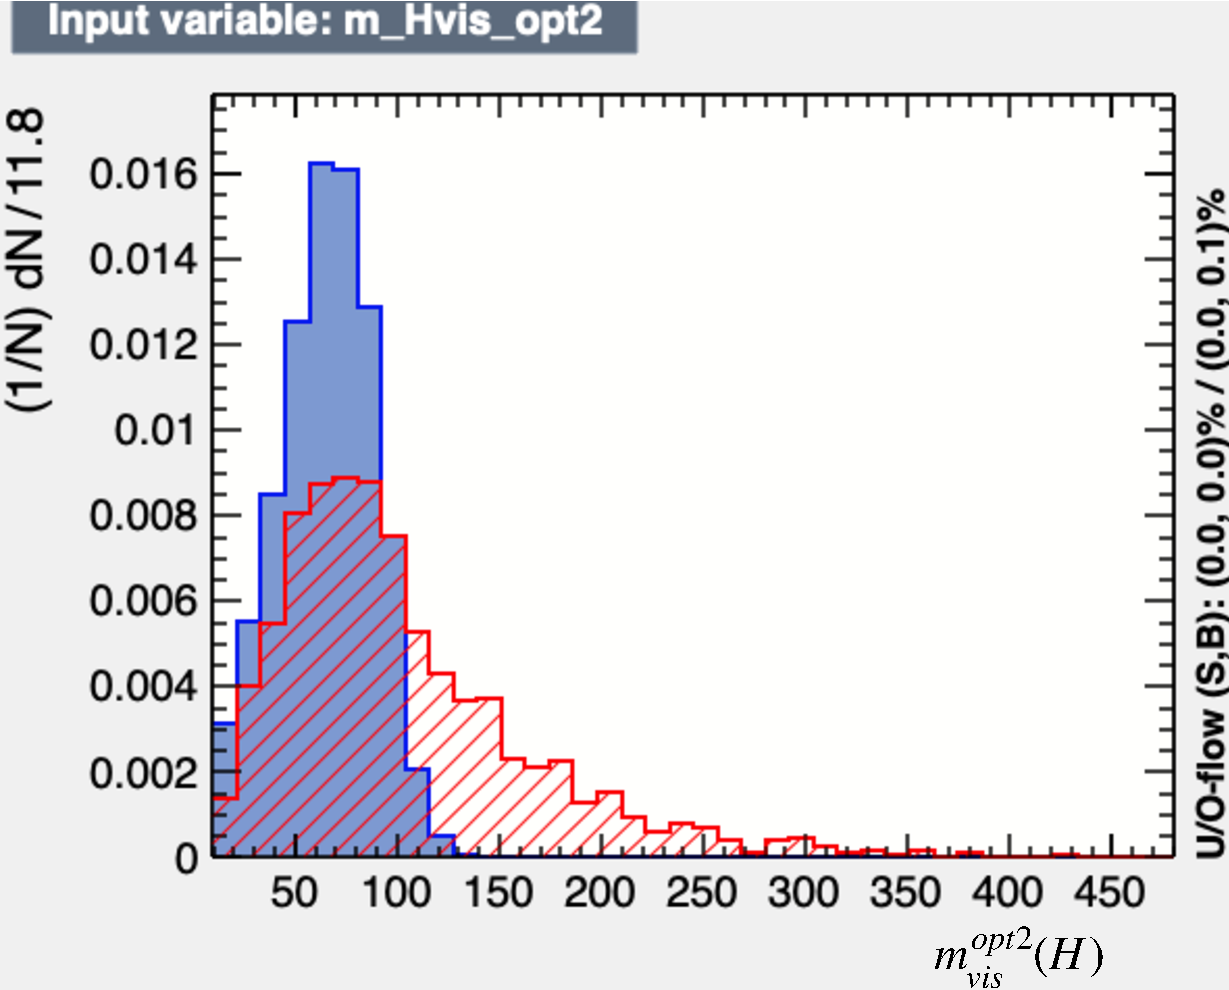
\includegraphics[width=.31\textwidth]{Chapter5_tHq/LeptAssociation/BDT_InputVariables/pdf_input_m_Hvis_opt2}
\caption{Input variables for the lepton assignment BDT. In blue the events in which the $\ell_{1}$ comes from the top quark decay
and in red those for which $\ell_{1}$ is produced from the Higgs boson. Note that only events that contain the truth-reco matching described 
in Section \ref{sec:tHq:origin:LeptonAssignment_truth_reco_DeltaRCone} are used to produce these plots.}
\label{fig:dileptau:Assignment_appendix:InputVars}
\end{figure}

Furthermore, it is important that the selected variables are not highly correlated, as correlations 
can exacerbate model complexity and result in redundant information that provides no improvement to model performance.
% Keep in mind that more complex models can be harmful since the computational times to operate the model increase and
% High correlations can lead to overfitting, where the model becomes too complex and 
% performs well on the training set but poorly on new, unseen data.
Figure \ref{fig:dileptau:Assignment_appendix:InputVars:Correlations} present the 
correlation matrices for the final input variables. A correlation matrix is a square 
matrix that provides a comprehensive view of the correlation coefficients between 
multiple variables. Note that these matrices show the bidimensional linear correlation coefficients
but the BDT uses N-dimensional relations so relevant higher order relations cannot be
uncovered by the matrices.

When using larger sets of input features, as expected, an increase in the number 
of highly correlated pairs of variables is observed. To address this concern, for each 
correlated variable pair, the variable with lower separation power, as determined by 
the BDT, is removed from the analysis.

Note that in Figure \ref{fig:dileptau:Assignment_appendix:InputVars:Correlations} 
there are still some pairs of collinear variables such as $m^{opt2}_{pred}(t)$ and 
$\Delta R(b\text{-taged jet}, \ell_{2})$. One could think that one of these two should 
be eliminated from the model but since the correlation is only present in one 
category (Type$\,$1 in this case) it can still be used because provides identification
power in the other.

\begin{figure}
\centering
\begin{subfigure}[b]{0.75\textwidth}
   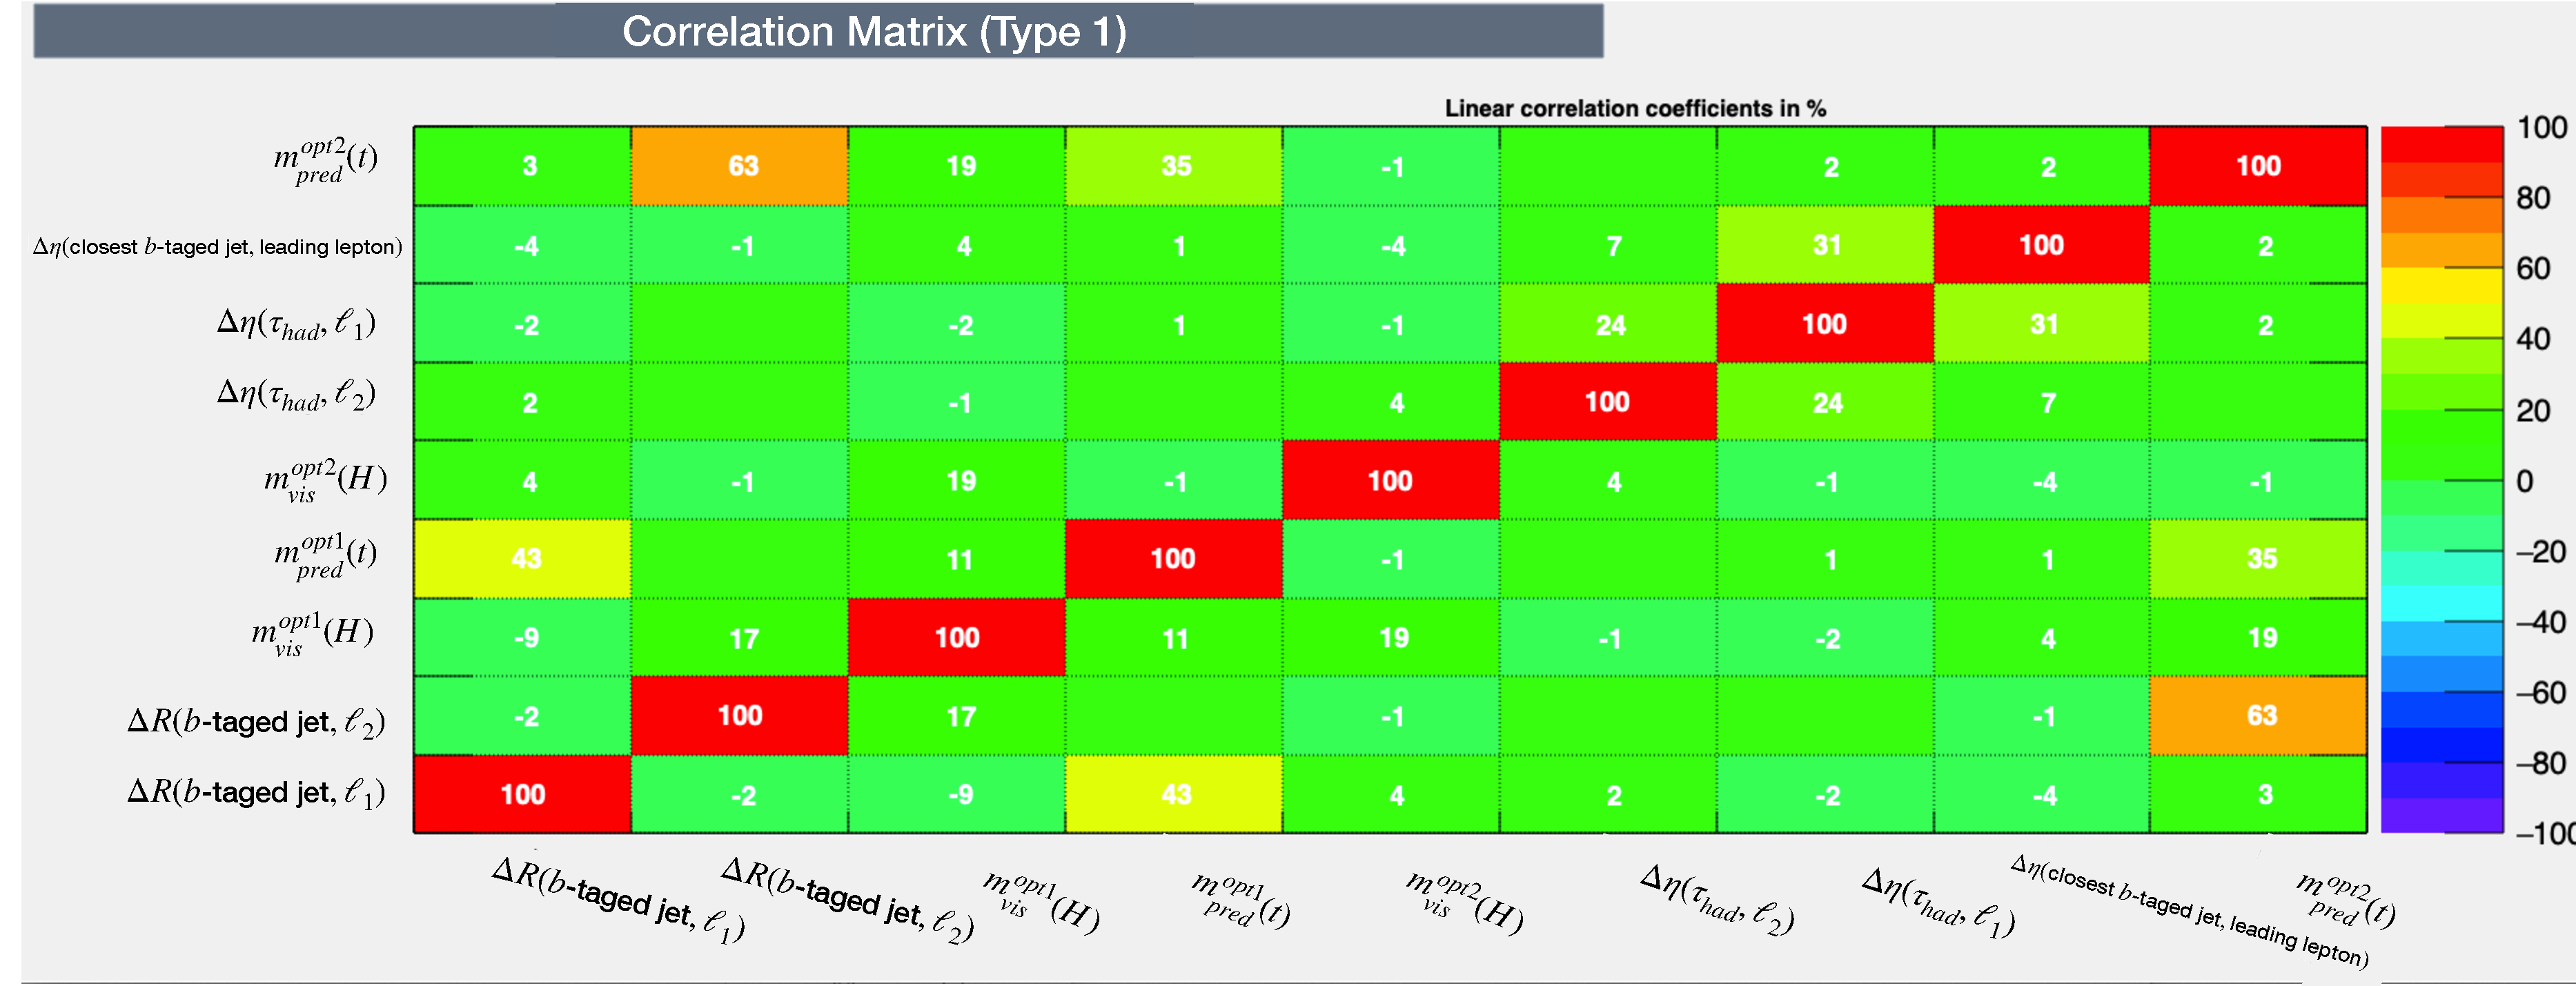
\includegraphics[width=1\linewidth]{Chapter5_tHq/LeptAssociation/BDT_InputVariables/pdf_0_input_correlations_Type1}
   \caption{Events with $\ell_{1}$ form top and $\ell_{2}$ from Higgs.}
   \label{fig:dileptau:Assignment_appendix:InputVars:Correlations:Type1} 
\end{subfigure}
\begin{subfigure}[b]{0.75\textwidth}
   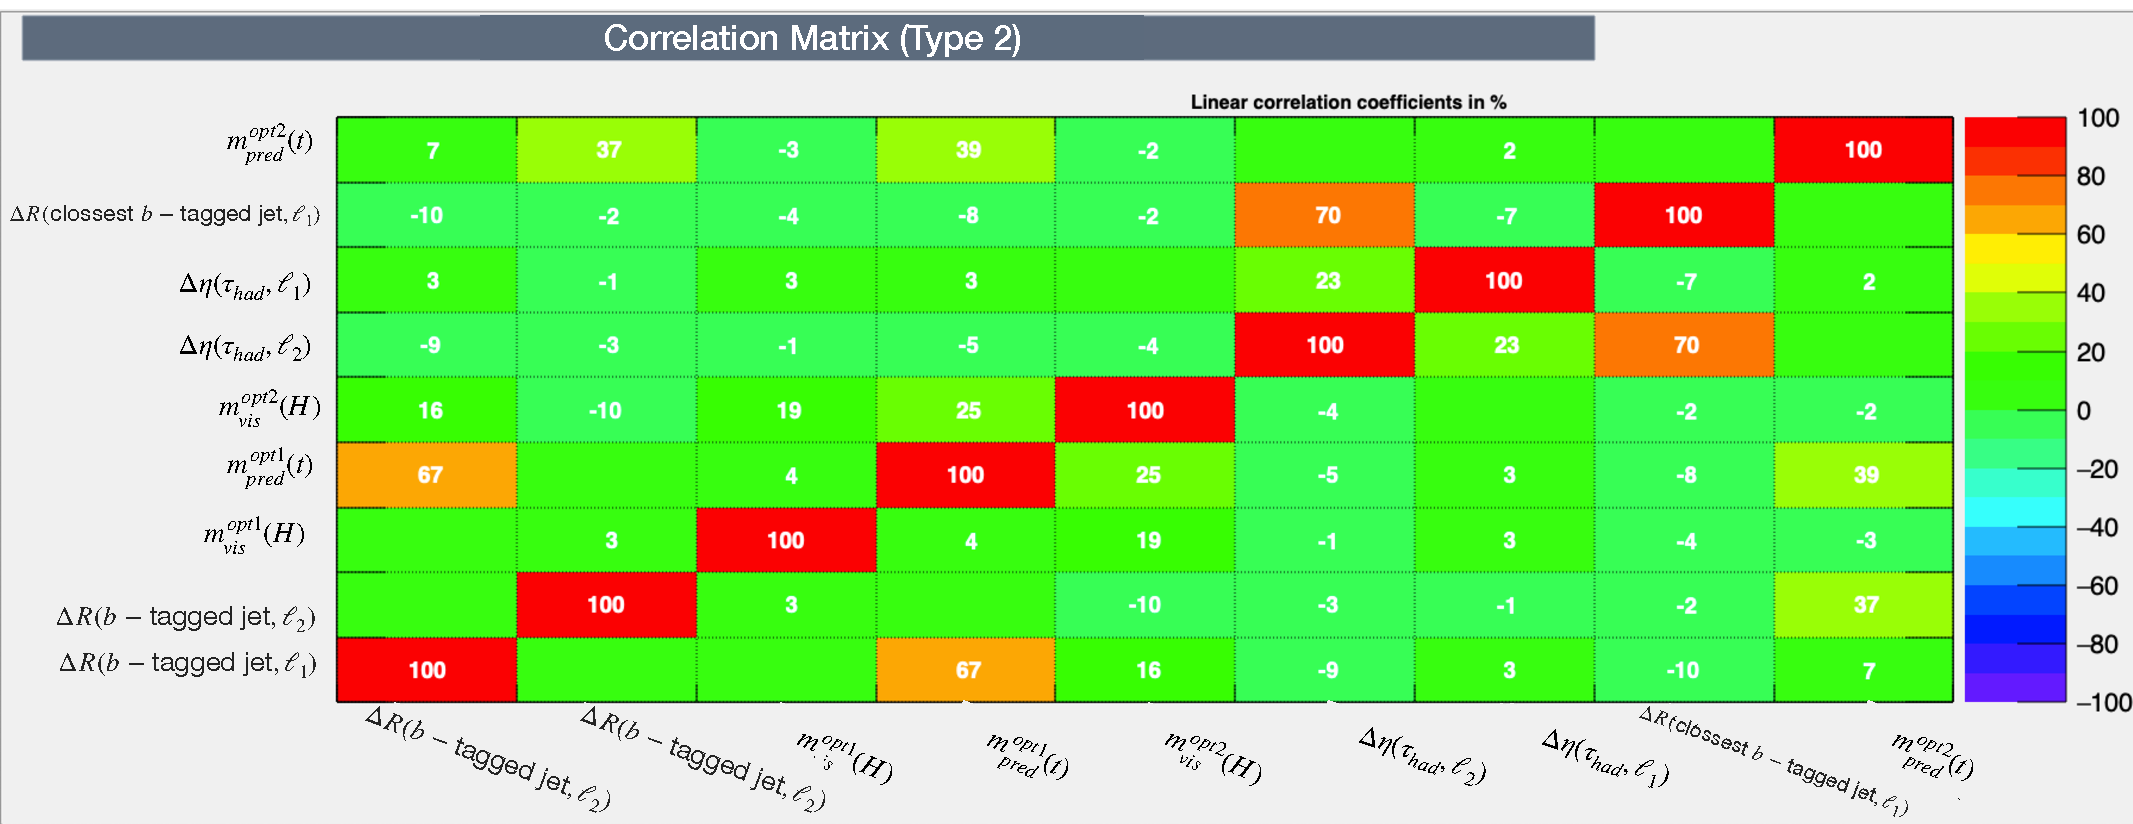
\includegraphics[width=1\linewidth]{Chapter5_tHq/LeptAssociation/BDT_InputVariables/pdf_0_input_correlations_Type2}
   \caption{Events with $\ell_{1}$ form Higgs and $\ell_{2}$ from top}
   \label{fig:dileptau:Assignment_appendix:InputVars:Correlations:Type2}
\end{subfigure}
\caption{Matrices showing the linear correlation coefficients of the BDT input variables for the Type$\,$1 
and Type$\,$2 samples. The correlation coefficients range from -100 to 100, being 0 the value for 
totally independent variables. Higher order functional or non-functional
relationships may not, or only marginally, be reflected in the value of linear correlation coefficient.}
\label{fig:dileptau:Assignment_appendix:InputVars:Correlations} %(See page 26 of the TMVA guide)
\end{figure}

TMVA.ROOT is capable of ranking variables within its model based on their separation 
power\footnote{See Eq. \ref{eq:Appendix:BDT:SeparationPower} in Appendix \ref{chap:Appendix:BDT} for more details.}
 ($<S^{2}>$). 
The variables employed in the model, ordered according to their respective levels of importance, are as follows:
\begin{itemize}
   	\item $m^{opt1}_{vis}(H)$: Mass of the combined hadronic tau and the 
		leading light-lepton. %m\_Hvis\_opt1
		 $<S^{2}> = 3.734 \times 10^{-01}$.
   	\item $\Delta \eta(\tauhad, \ell_{1})$: $\Delta \eta$ between the 
		hadronic tau and the leading light-lepton. %deltaEta\_tau\_LightLep1
		 $<S^{2}> = 2.457 \times 10^{-01}$.
    	\item $m^{opt2}_{vis}(H)$: Mass of the combined hadronic tau and 
		the sub-leading light-lepton. %m\_Hvis\_opt2
		 $<S^{2}> = 2.025 \times 10^{-01}$.
   	\item $\Delta \eta(\tauhad, \ell_{2})$: $\Delta \eta$ between the 
		hadronic tau and the sub-leading light-lepton. %deltaEta\_tau\_LightLep2
		 $<S^{2}> = 1.864 \times 10^{-01}$.
    	\item $m^{opt1}_{pred}(t)$: Mass of the top quark when reconstructed 
		as the sum of the $b$-jet and the leading light-lepton.  %m\_Tpred\_opt1
		 $<S^{2}> = 1.596 \times 10^{-01}$.
    	\item $\Delta R(b\text{-taged jet}, \ell_{1})$: $\Delta R$ between the 
		$b$-tagged jet and the leading light-lepton. %deltaR\_b\_LightLep1        
		 $<S^{2}> = 1.142 \times 10^{-01}$.
    	\item $m^{opt2}_{pred}(t)$: Mass of the top quark when reconstructed 
		as the sum of the $b$-jet, the sub-leading lepton and the prediction for the neutrino
		of the $\ell_{2}$. %$m_{pred}(t) = \sqrt{(P_{b}+P_{\ell}+P_{\nu, pred})^}{2}$%m\_Tpred\_opt2
		 $<S^{2}> = 1.104 \times 10^{-01}$.
	\item $\Delta R(b\text{-taged jet}, \ell_{2})$: $\Delta R$ between the 
		$b$-tagged jet and the sub-leading light-lepton.%deltaR\_b\_LightLep2
		 $<S^{2}> = 1.009 \times 10^{-01}$.
    	\item $\Delta \eta(\text{closest }b\text{-taged jet}, \text{leading lepton})$: 
		$\Delta \eta$ between the leading lepton and the closest $b$-tagged 
		jet to that lepton.%¿?This lepton can either be a light lepton or the hadronic tau.
		%DeltaEtaLeadingLeptonClosestBjet			
		 $<S^{2}> = 7.401 \times 10^{-02}$.
\end{itemize}
The ranking of the BDT input variables is derived by counting how often the variables are used to 
split decision tree nodes. Then each split occurrence is weighted by the separation gain-squared 
it has achieved and by the number of events in the node \cite{Breiman1984ClassificationAR}.
% source: 8.13.4 https://root.cern.ch/download/doc/tmva/TMVAUsersGuide.pdf
% source references: L. Breiman, J. Friedman, R. Olshen and C. Stone, “Classification and Regression Trees”, Wadsworth (1984).

Numerous other variables were examined but were not integrated into the model due to several reasons.
 Some of these variables were not relevant in terms of separation, while others displayed a strong correlation 
 with another variable that was already included in the model.

%Additionally, the decision to not incorporate additional input features into the model was influenced 
%by the fact that a separate BDT is used to distinguish between signal and background processes 
%(as described in Section \ref{sec:ChaptH:EventSelection}). 

Other reason to not incorporate more input features into the model is that another BDT is later used for separating
signal from the background processes (Section \ref{sec:ChaptH:EventSelection}) and this region-definition BDT uses
as input the variables filled with output of the lepton-assignment BDT. One shall be careful when doing this because
using the same variables in both BDTs can lead to biases. Let's refer to the second BDT as the
region-definition BDT in contrast to the lepton-assignment BDT.
%This region-definition BDT includes variables that are built using the outcome of the lepton-assignment BDT
%and, hence, caution must be taken as double-using the same variables within a BDT can result in biases.


 %%%%%%%%%%%%%%%%%%
%           BDT-Hyperparameters     %
%%%%%%%%%%%%%%%%%%
\subsubsection{Optimisation of the lepton-assignment BDT hyperparameters}
\label{sec:ChaptH:Sig:LepAsign:SS:BDT:hyperparameters}
The hyperparameters are the parameters whose values control the learning process.
They are not part of the final model but determine the values of the model parameters that
the learning algorithm acquires. The search of the optimal hyperparameters is fundamental 
when seeking to develop a model that exhibits a high level of performance. 
While certain machine learning libraries such as PyTorch, scikit-learn, XGBoost, and TensorFlow, 
offer functionality for discovering the most effective hyperparameter values, 
the corresponding capabilities within ROOT.TMVA remain in a developmental stage, 
and presently, they are not even documented. Tests have been carried to identify optimal 
hyperparameters using a genetic algorithm, with the ROC area serving as the primary figure of merit. 
However, better performances are achieved through the manual fine-tuning of hyperparameters.

A discussion about the different hyperparameters and its meaning is provided 
in the Appendix \ref{fig:Appendix:BDT:Hyperparams}. The set of hyperparameters 
used to train the model is present in the Table \ref{tab:chap:tH:LepAssign:Hyperparams}.

\begin{table}[htbp!]
\centering
\begin{tabular}{l|l|l}
\toprule
Hyperparam.	   			& Value  				& Meaning                               \\ 
\midrule
\texttt{MaxDepth} 			& 3      				& Maximum depth of cell tree.            \\
\texttt{Shrinkage}			& 0.2    				& Learning rate for GradBoost algorithm. \\
\texttt{NTrees}    			& $10^3$ 				& Number of trees in method.             \\
\multirow{2}{*} {\texttt{nCuts}} 	& \multirow{2}{*}{40} 		& Number of grid points in variable range used. \\
		  				&					& in finding optimal cut in node splitting. \\
\bottomrule
\end{tabular}
\caption{Hyperparameters tuned for the lepton-assignment BDT training. 
The rest of hyperparameters were set to its default values. 
More details about this can be found in Appendix \ref{fig:Appendix:BDT:Hyperparams} . The hyperparameter 
NegWeightTreatment is discussed in Section \ref{sec:ChaptH:Sig:LepAsign:SS:BDT:NegWeights}.}
\label{tab:chap:tH:LepAssign:Hyperparams}
\end{table}

 %%%%%%%%%%%%%%
%        BDT-NegWeight     %
%%%%%%%%%%%%%%
\subsubsection{Treatment of the negatively weighted events}
\label{sec:ChaptH:Sig:LepAsign:SS:BDT:NegWeights}
Negatively weighted events can pose challenges when using a BDT or other ML techniques 
such as NN. These issues are discussed with more detail in Section \ref{chap:Appendix:BDT:NegWeigts}.
The origin of the negatively weighted events is explained in \ref{chap:Appendix:NegWeights:intro}.


When training BDT, it is necessary to address the issue of negatively weighted events since it
cannot directly handle negative weights. Two common approaches to handle this situation are: 
ignoring negative weights during training and using the absolute values of the weights. 

In the case of ignoring negative weights during training, the BDT algorithm treats all 
events with negative weights as if they have zero weight (i. e. its information is lost). 
This approach avoids any potential complications arising from negative weights but 
still preserves the positively weighted events in the training process. On the other hand, 
using the absolute values of the weights involves taking the magnitude of the negative weights, 
effectively treating them as positive weights. This second strategy allows the BDT to 
incorporate the information from these events while disregarding the sign of the weights.

Other options are provided by the ROOT TMVA library, as described in Section
\ref{chap:Appendix:BDT:NegWeigts:TMVARoot}. However, after conducting several tests, 
it was observed that these alternative techniques did not exhibit comparable performance 
in terms of both separation power and stability when compared to the approach of ignoring 
negative weights.

After careful evaluation and experimentation, it was determined that excluding events with 
negative weights yielded better results than using the absolute weights of the events. This 
approach demonstrated improved performance in terms of the desired outcomes of the BDT training.

However, to ensure the validity of this approach, it is crucial to verify that the subset of positively 
weighted events accurately represents the behaviour of the data. Approximately 40\% of the signal 
entries have negative weights and, hence, ignoring this part could affect distribution of the samples. 
Therefore, before discarding these events during training, it is necessary to examine whether the 
shape of the data distributions is significantly affected.

In Figure \ref{fig:dileptau:Assignment_appendix:NegativeWeights}, we compare the distributions' shapes 
using all events versus using only positively weighted events. As shown, the variable distributions exhibit 
perfect compatibility within the error bands. Additionally, the concentration of negative weights is practically 
the same for both categories, with 36.1\% for  Type$\,$1 and 36.6\% for Type$\,$2. This indicates a balanced
 representation, as removing negative weights does not introduce bias towards either category.

In conclusion, using only the positively weighted events in the training 
process does not present any significant issue.

\begin{figure}[htbp!]
\centering
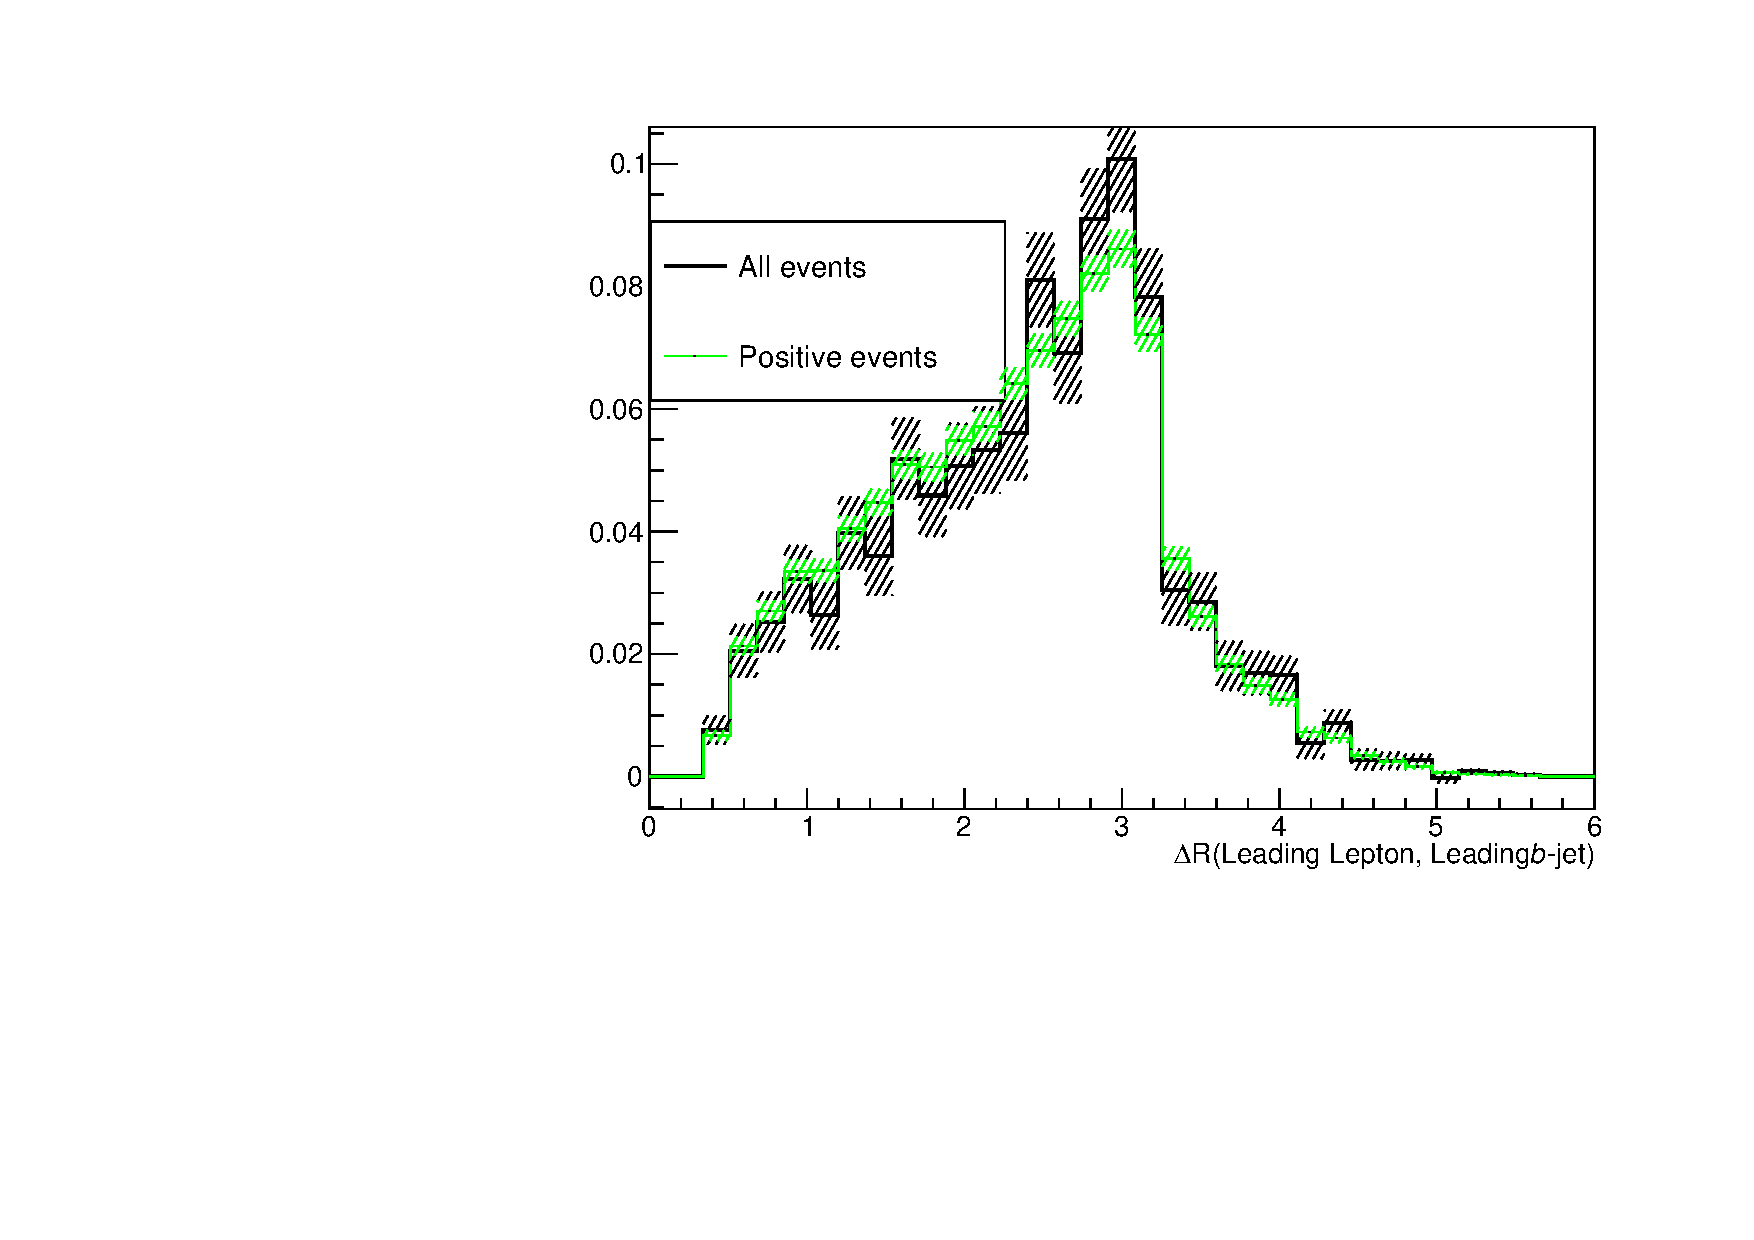
\includegraphics[width=.31\textwidth]{Chapter5_tHq/LeptAssociation/NegativeWeights/PosVsAll_SS_err_deltaR_b_LightLep1}\quad
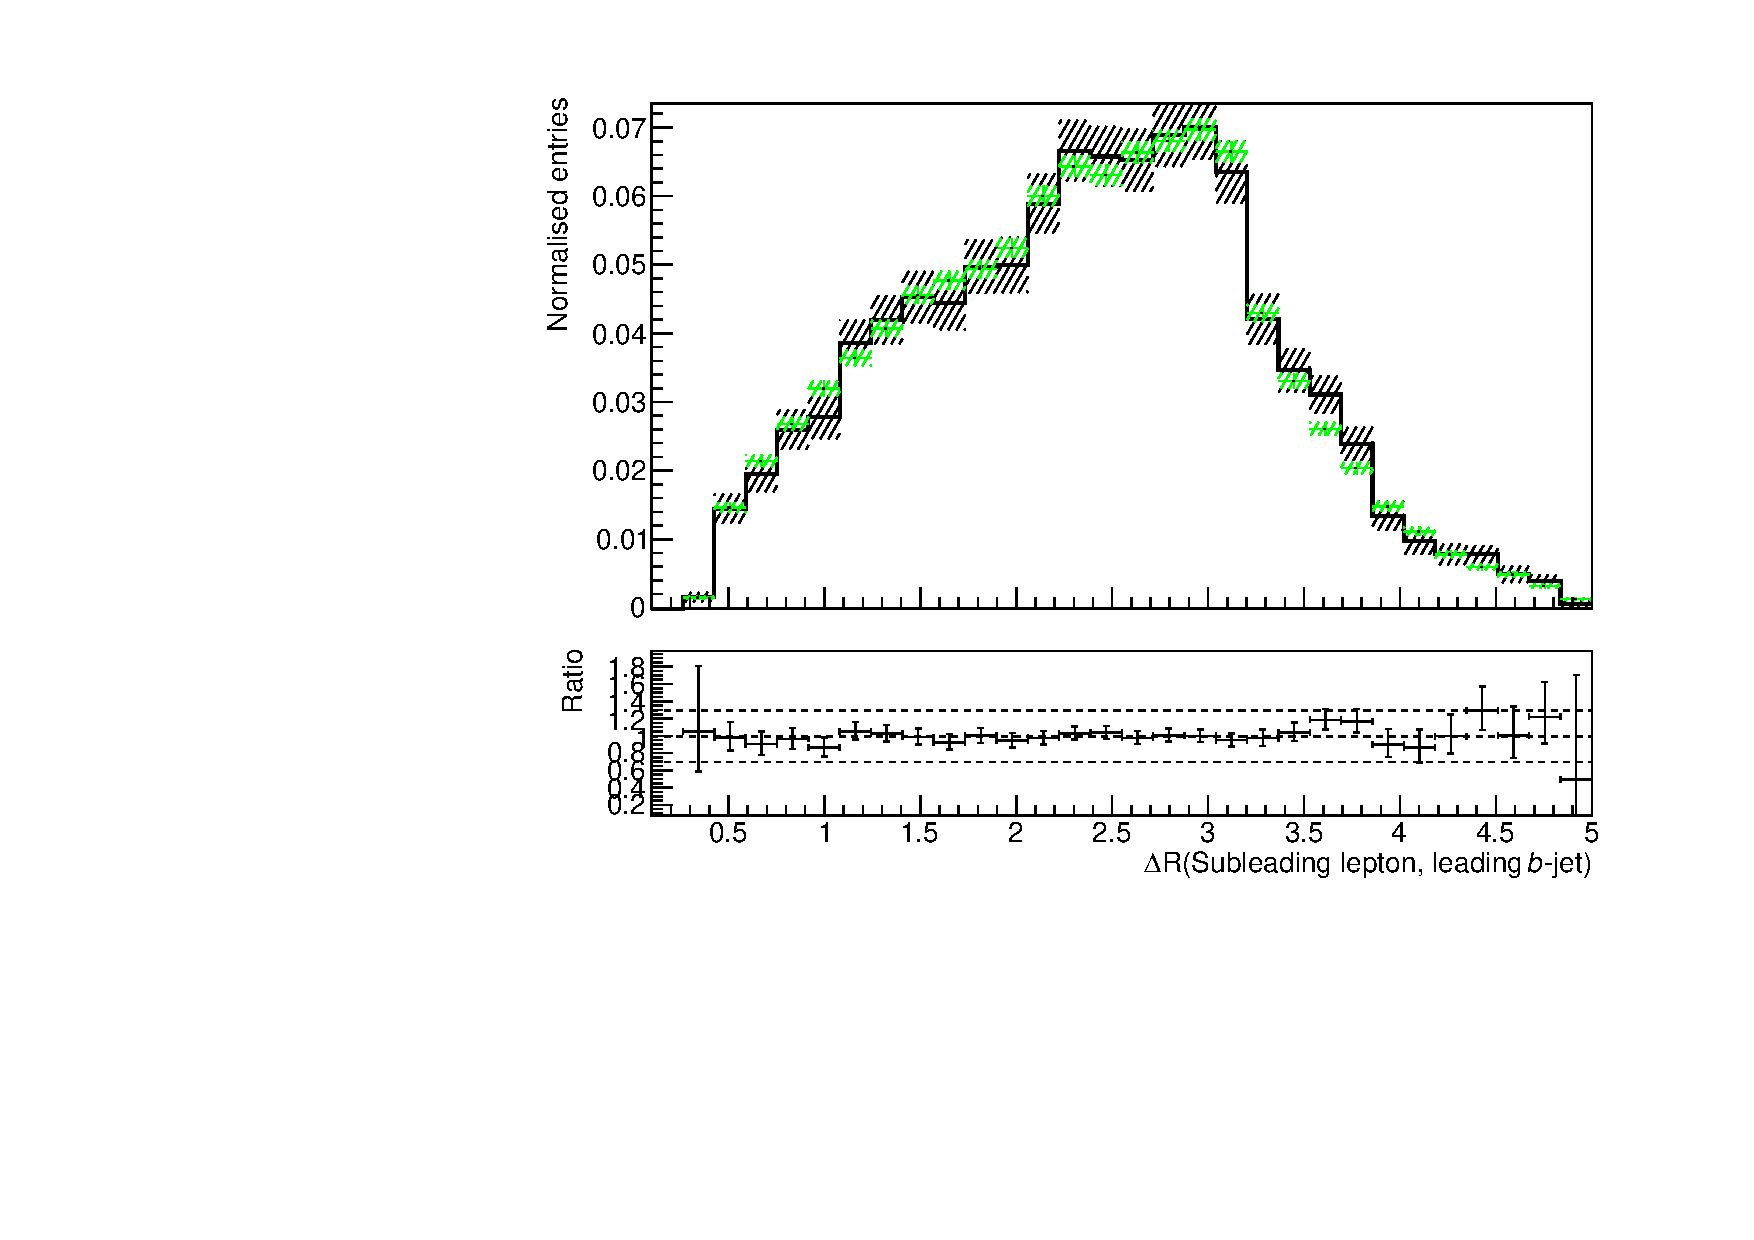
\includegraphics[width=.31\textwidth]{Chapter5_tHq/LeptAssociation/NegativeWeights/PosVsAll_SS_err_deltaR_b_LightLep2}\quad
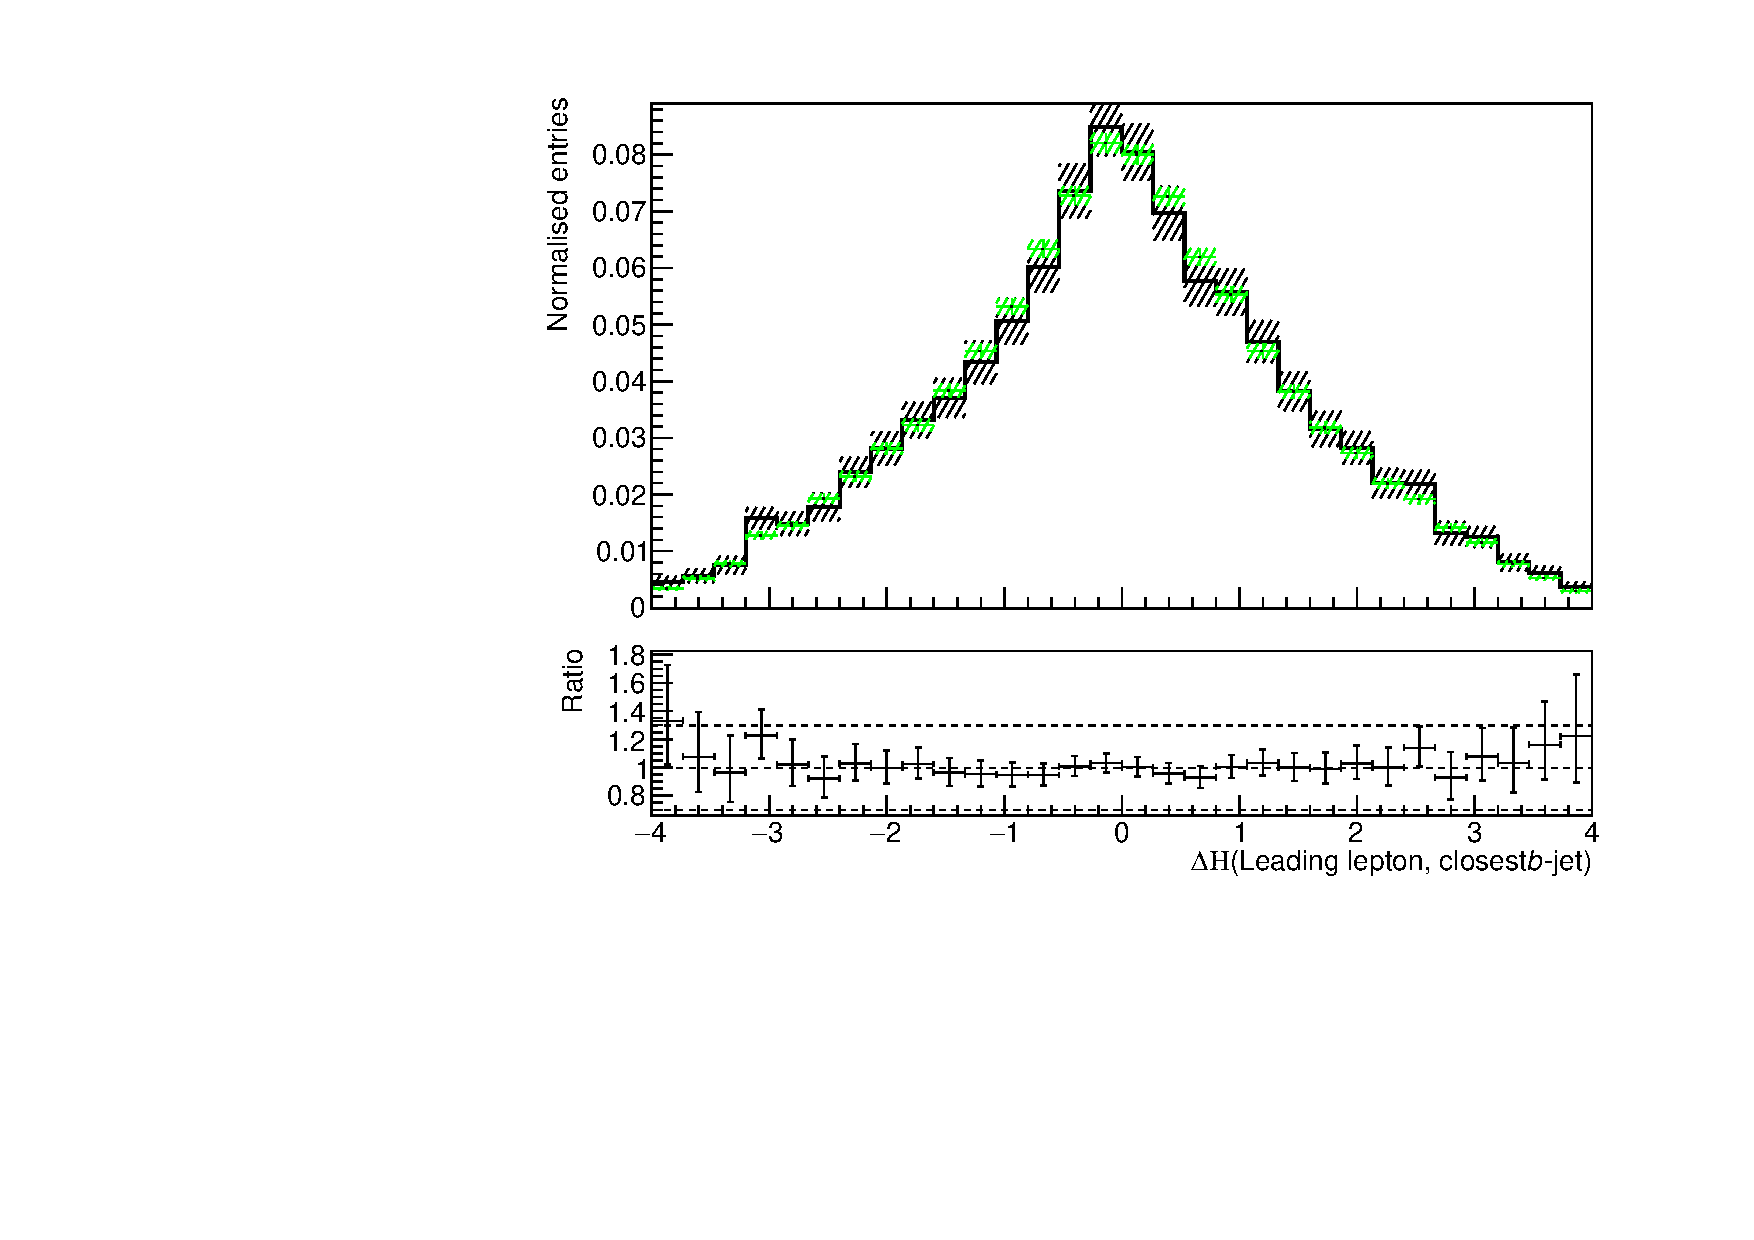
\includegraphics[width=.31\textwidth]{Chapter5_tHq/LeptAssociation/NegativeWeights/PosVsAll_SS_err_DeltaEtaLeadingLeptonClosestBjet}
\medskip
\includegraphics[width=.31\textwidth]{Chapter5_tHq/LeptAssociation/NegativeWeights/PosVsAll_SS_err_deltaEta_tau_LightLep1}\quad
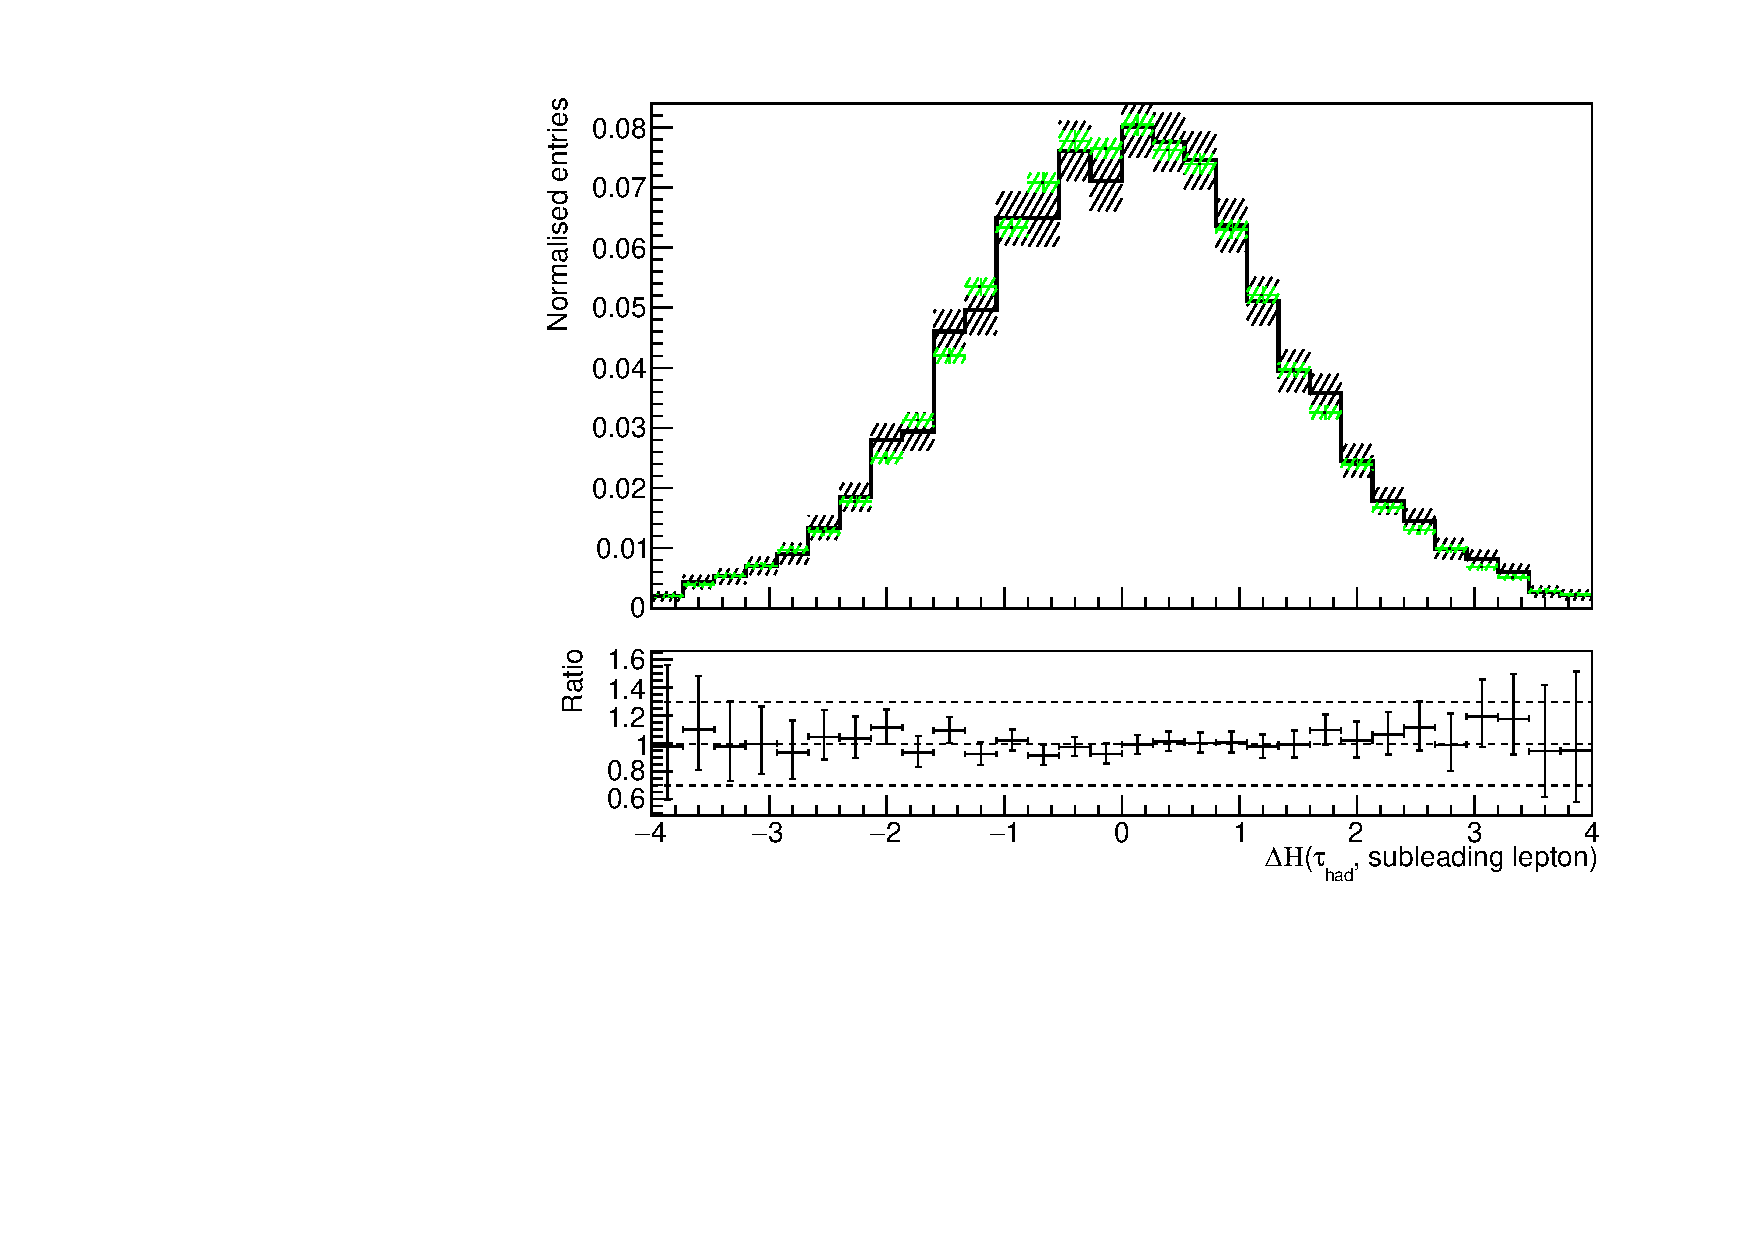
\includegraphics[width=.31\textwidth]{Chapter5_tHq/LeptAssociation/NegativeWeights/PosVsAll_SS_err_deltaEta_tau_LightLep2}\quad
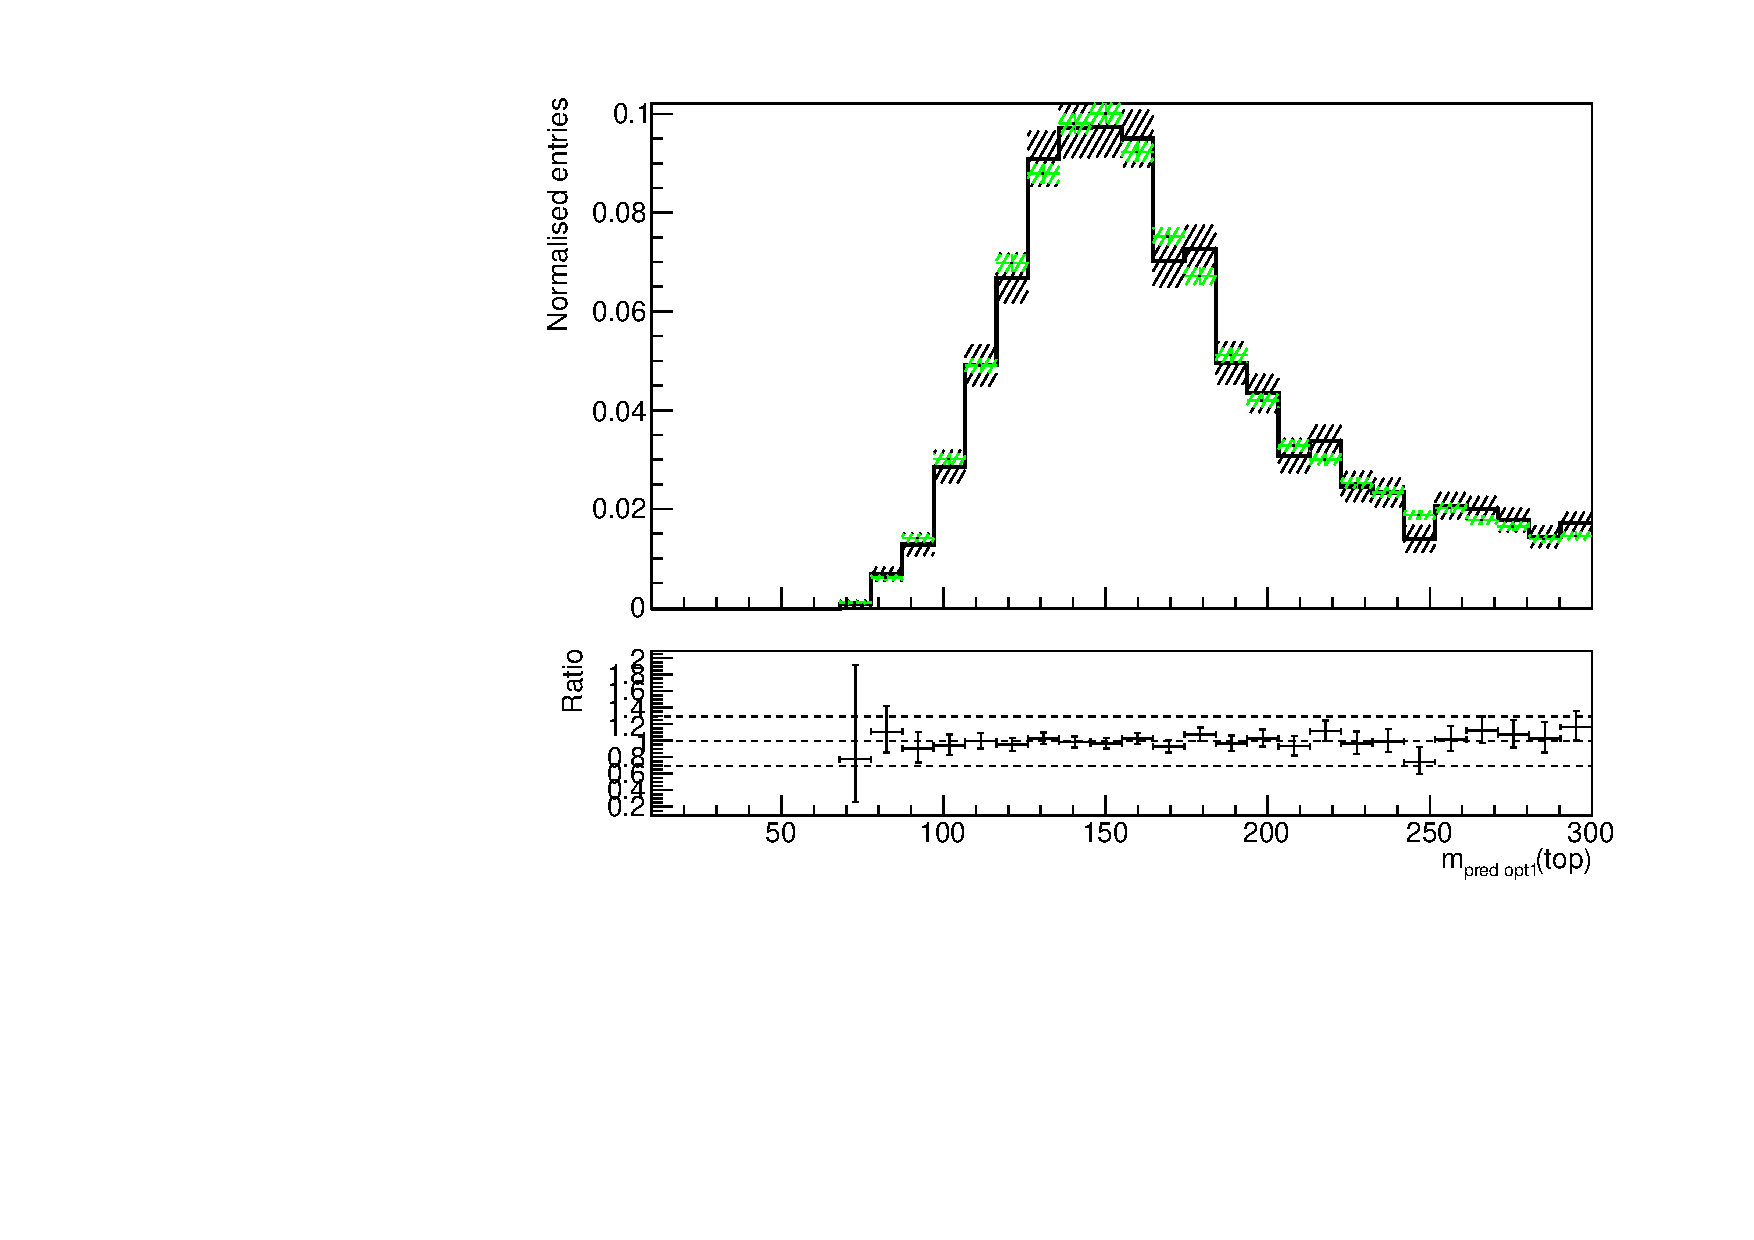
\includegraphics[width=.31\textwidth]{Chapter5_tHq/LeptAssociation/NegativeWeights/PosVsAll_SS_err_m_Tpred_opt1}
\medskip
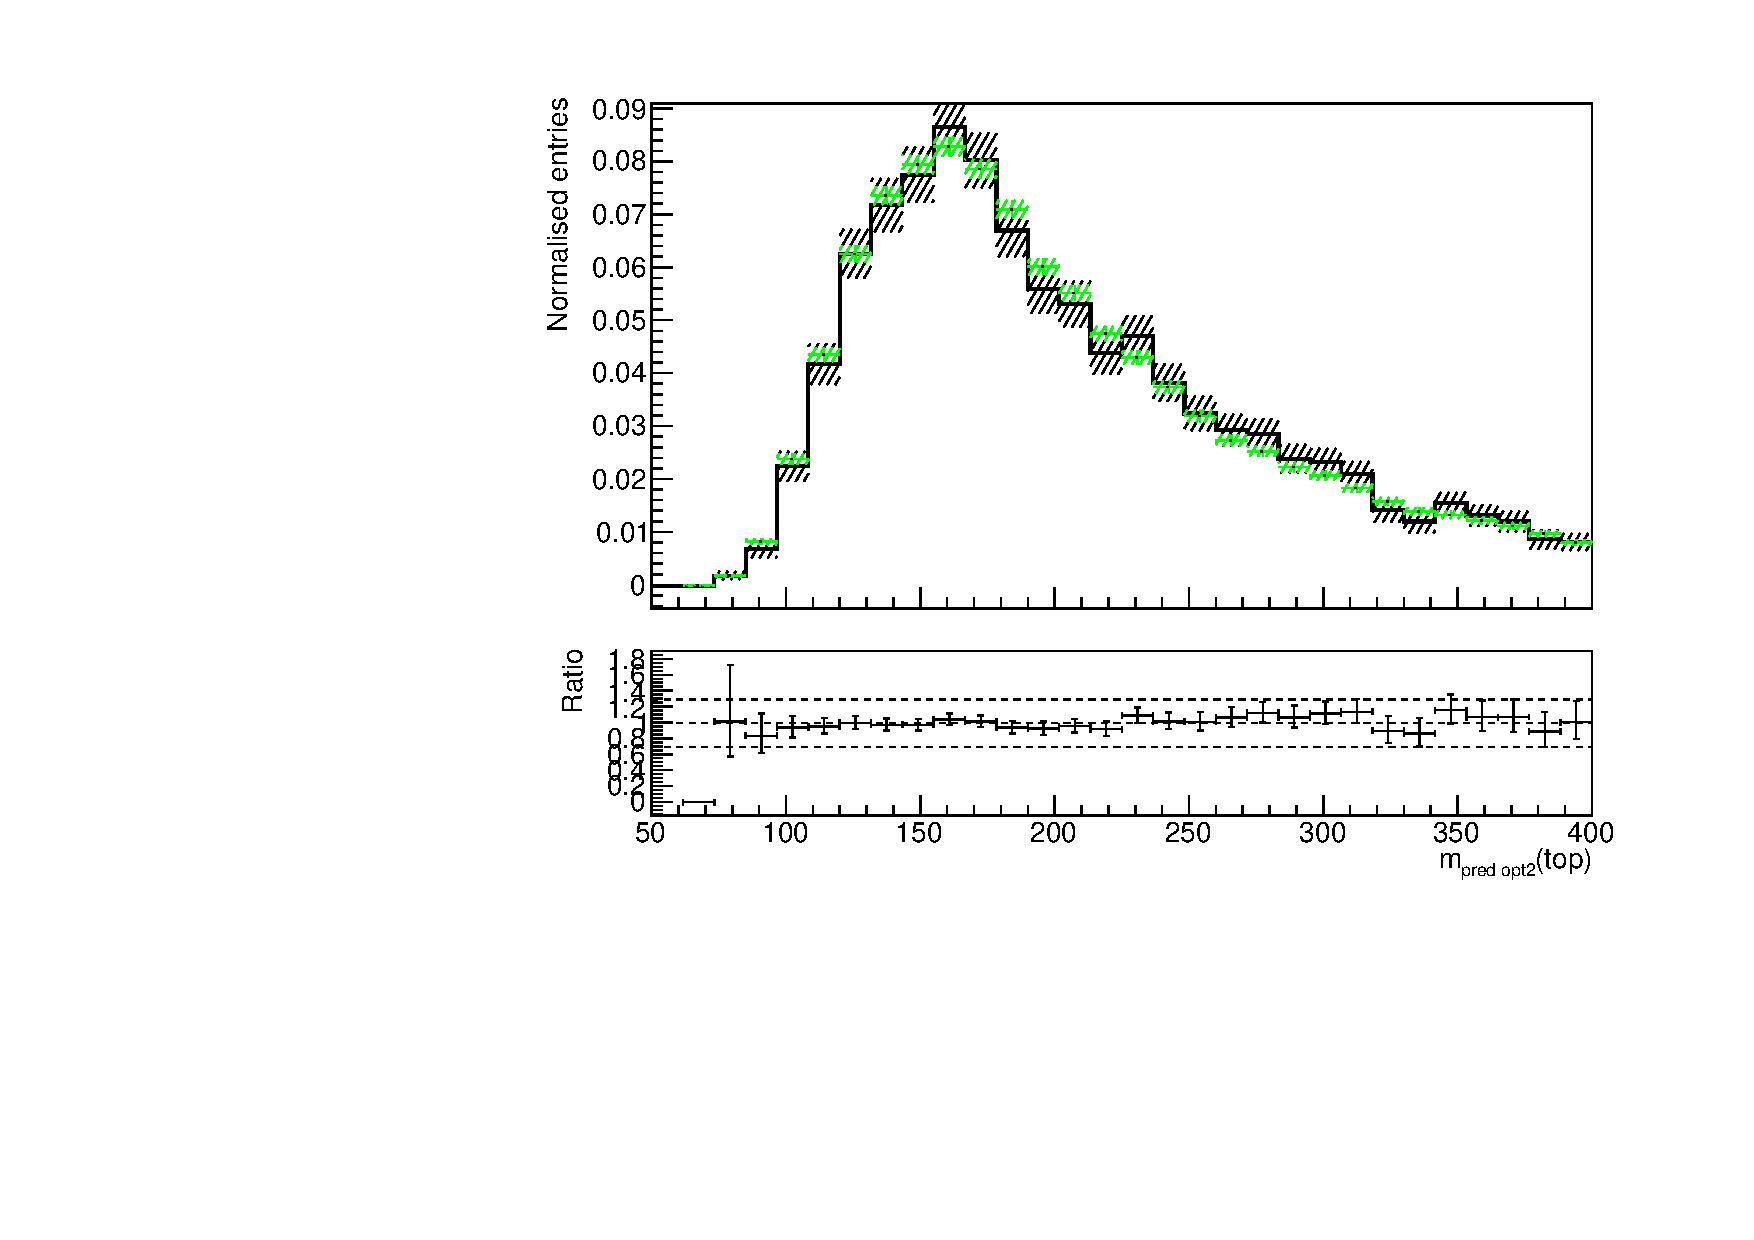
\includegraphics[width=.31\textwidth]{Chapter5_tHq/LeptAssociation/NegativeWeights/PosVsAll_SS_err_m_Tpred_opt2}\quad
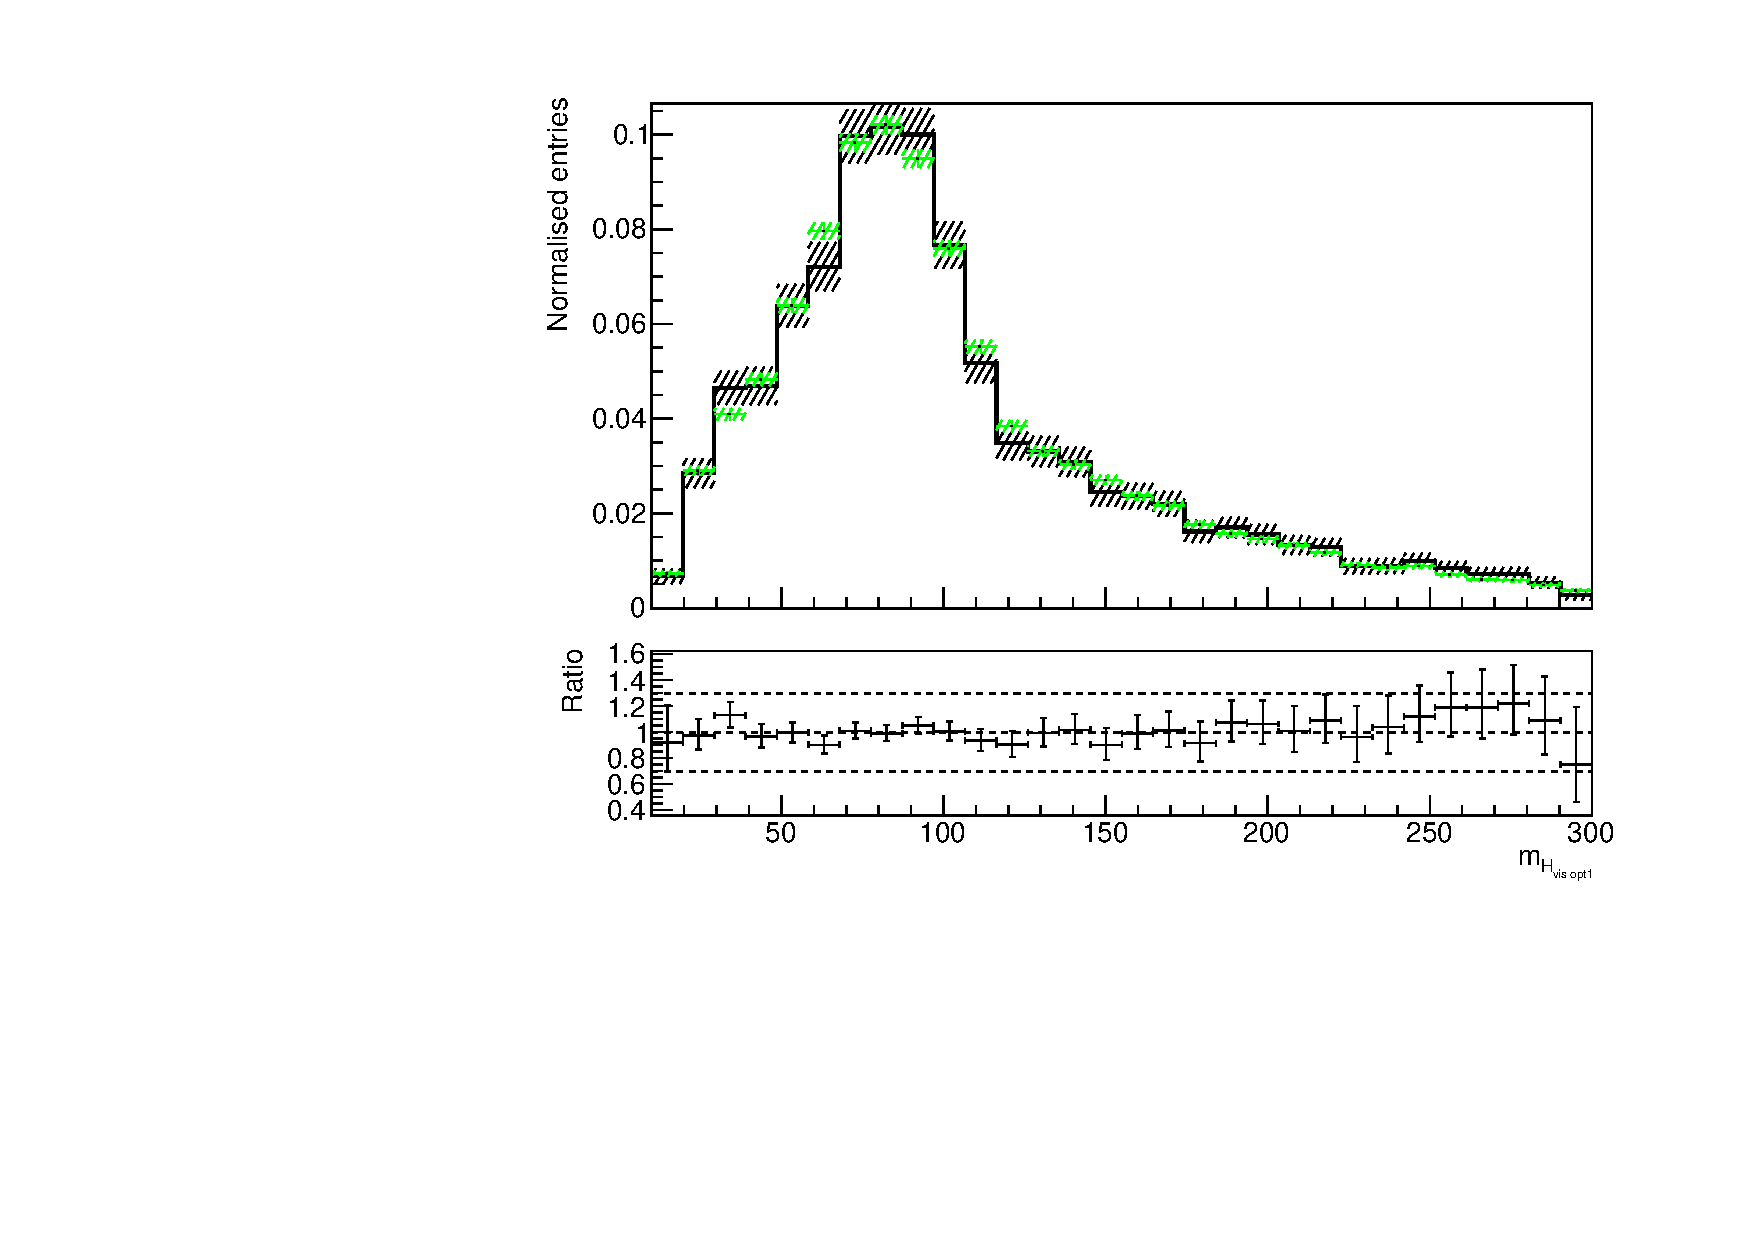
\includegraphics[width=.31\textwidth]{Chapter5_tHq/LeptAssociation/NegativeWeights/PosVsAll_SS_err_m_Hvis_opt1}\quad
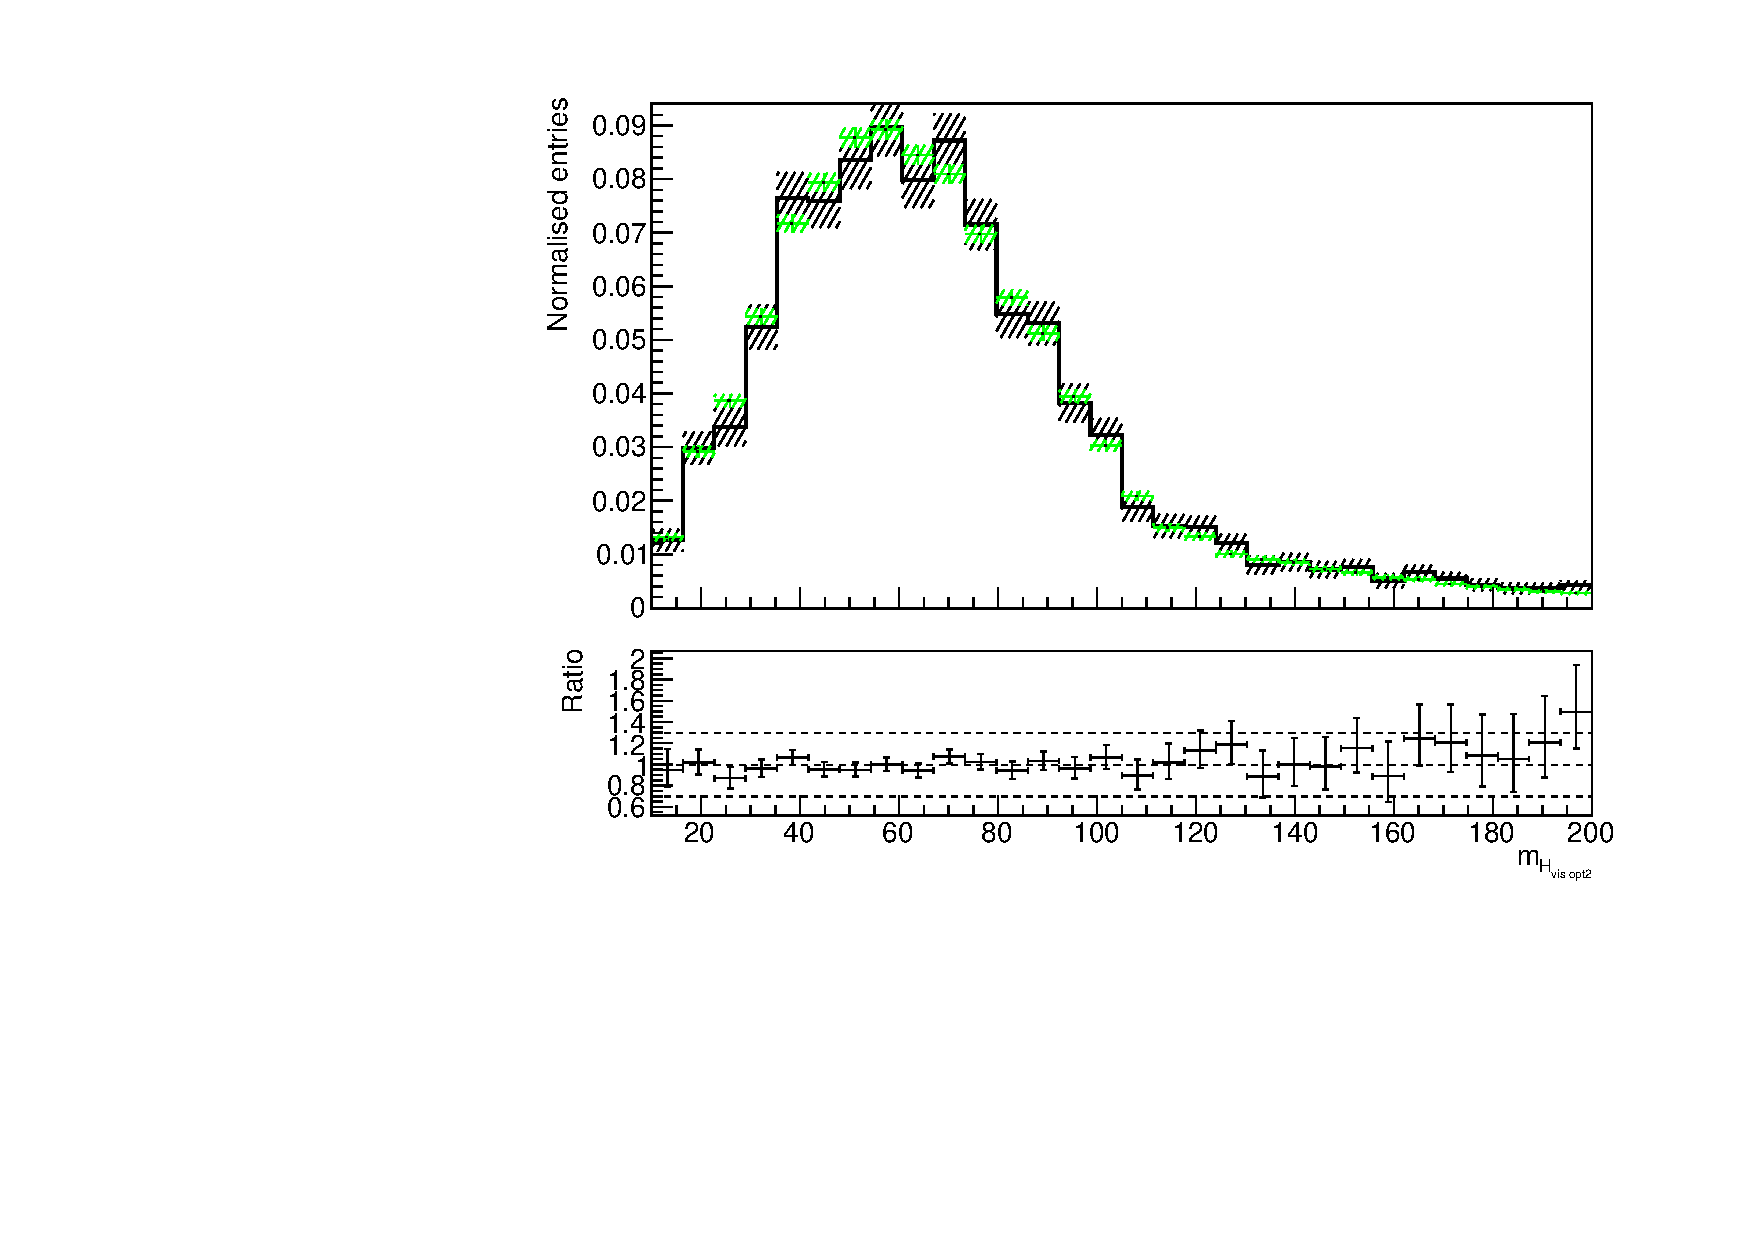
\includegraphics[width=.31\textwidth]{Chapter5_tHq/LeptAssociation/NegativeWeights/PosVsAll_SS_err_m_Hvis_opt2}
\caption{Normalised distributions of the BDT input variables for the \dilepSStau samples. 
The distributions using all events (black) and using only the positively-weighted ones (green)
are superimposed. The error bands correspond to the statistical error. 
Note that the distributions have the same profile.}
\label{fig:dileptau:Assignment_appendix:NegativeWeights}
\end{figure}



%%%%%%%%%%%%%
%           BDT-Training    %
%%%%%%%%%%%%%
\subsubsection{Training of the lepton-assignment BDT}
\label{sec:ChaptH:Sig:LepAsign:SS:BDT:Training}
The primary objective of the lepton-assignment BDT is to differentiate 
between the Type$,$1 and Type$,$2 categories, similar to the separation 
of signal and background with the region-definition BDT. The variable 
\texttt{isLep1fromTop} is used to label these categories. One important
difference between the region-definition BDT and the lepton-assignment BDT
is that while the former is using all the sample, the later is exclusively trained 
on \dilepSStau signal events. This approach is justified by the objective of 
determining the origin of each lepton in the signal events, a classification 
that is meaningful only within the context of signal processes

%Therefore, the two classes are define as:
%	\begin{itemize}
%		\item  \textbf{Type 1}: The leading $\ell$ (\emu) comes from the top-quark decay chain and, hence, 
%				the sub-leading from the Higgs boson (\texttt{isLep1fromTop} =0). 
%				As expected, this is the most frequent type since
%				the top quark carries more momentum. 
%		\item  \textbf{Type 2}: Just the opposite to the type 1. In this case, the decay chain 
%				of the Higgs boson is the source of the leading lepton while the sub-leading comes
%				from the top quark. The leading light lepton is a product from the Higgs-boson-decay chain
%				(\texttt{isLep1fromTop} =0).
%	\end{itemize}
 
The use of ROOT.TMVA offers the advantage of directly 
working with the root-formatted NTuples, eliminating the need to 
convert them to numpy arrays or pandas dataframes.

%Nowadays most of ML frameworks (keras, pyTorch, scikit-learn, XGBooost, etc..) are based on python. 
%These libraries expect numpy arrays or panda data-frames as input, so the first thing to do 
%when using the analysis NTuples is to convert the ROOT data-frame. An advantage of using TMVA library of
%ROOT is that this data conversion is not necessary.

In order to mitigate the effects of low statistics, the \textit{k}-folding (carefully described in 
the Appendix \ref{chap:Appendix:BDT:kfold}) method from cross validation in implemented using five folds. 
Thus meaning that the data is split in five sub-sets named folds 
and five BDTs are trained. Each model uses four folds
for training and one for test, implying that for each BDT the train/test split is 80/20\%.
After removing the negatively weighted events, 9362 raw-events are used for building the model.
Of those 5518 are Type$\,$1 and 3844 Type$\,$2. So each of the five BDTs uses 7490 events
in the training and 1872 in the classification.
This cross-validation technique allows to use all the events in the dataset for the train. 
No validation dataset is used but the different models
 are compared and if all of them behave similarly, there is no overtraining. 
 
 Due to the use of \textit{k}-folding, the training of the lepton-assignment BDT results 
 in five distinct ML models. If overtraining had occurred, these models would not 
 generalise effectively, leading to noticeable differences in the BDT score\footnote{The 
 score of the BDT is the result of the model prediction for a given event.} distributions 
 between models. Therefore, it is crucial to ensure that the models are consistent 
 with one another.
 
 \begin{figure}[htbp!]
	\begin{subfigure}[h]{0.45\linewidth}
		\includegraphics[width=\linewidth]{Chapter5_tHq/LeptAssociation/dileptau_LepAssignment_BDT_Score_ALL_train_GoodLegend.pdf}
		\caption{Events when used in the training set.}
	\end{subfigure}
	\hfill
	\begin{subfigure}[h]{0.45\linewidth}
		\includegraphics[width=\linewidth]{Chapter5_tHq/LeptAssociation/dileptau_LepAssignment_BDT_Score_ALL_test_GoodLegend.pdf}
		\caption{Events when used in the test set.}
	\end{subfigure}%
	\caption{Comparison of the profiles of the lepton-origin-assignment-BDT scores for the different models. 
	Observe that the scores exhibit similar distribution shape, indicating that 
	the model is not affected by the particular subset of data used for training.}
	\label{fig:ChaptH:dileptau:Assignment:ScoreDistributions}
\end{figure}

Figure \ref{fig:ChaptH:dileptau:Assignment:ScoreDistributions} displays the BDT 
score distributions for all five folds simultaneously. The purpose of this visualisation 
is to assess the compatibility of the five models and verify the absence of overtraining. 
As observed in the figure, the BDT score distributions are consistent across the folds, 
indicating that there is no evidence of overtraining.


Additionally, it is essential to compare the distributions of the train and test 
samples for each model. The greater the similarity between these distributions, 
the better the model's performance. However, it is crucial to note that an exact 
agreement between the train and test samples could indicate a potential bug or 
issue with the model.
Figure \ref{fig:dileptau:Assignment_appendix:ScoreDistributions} presents the 
BDT score distributions, simultaneously displaying the train and test samples 
while distinguishing between the two event types. This analysis is performed 
for all folds, each of them in a subfigure. By examining the figure, it can be 
observed that the train and test samples exhibit compatibility, indicating that the 
models are performing well and are not overfitting to the training data.


\begin{figure}[htbp!]
\centering
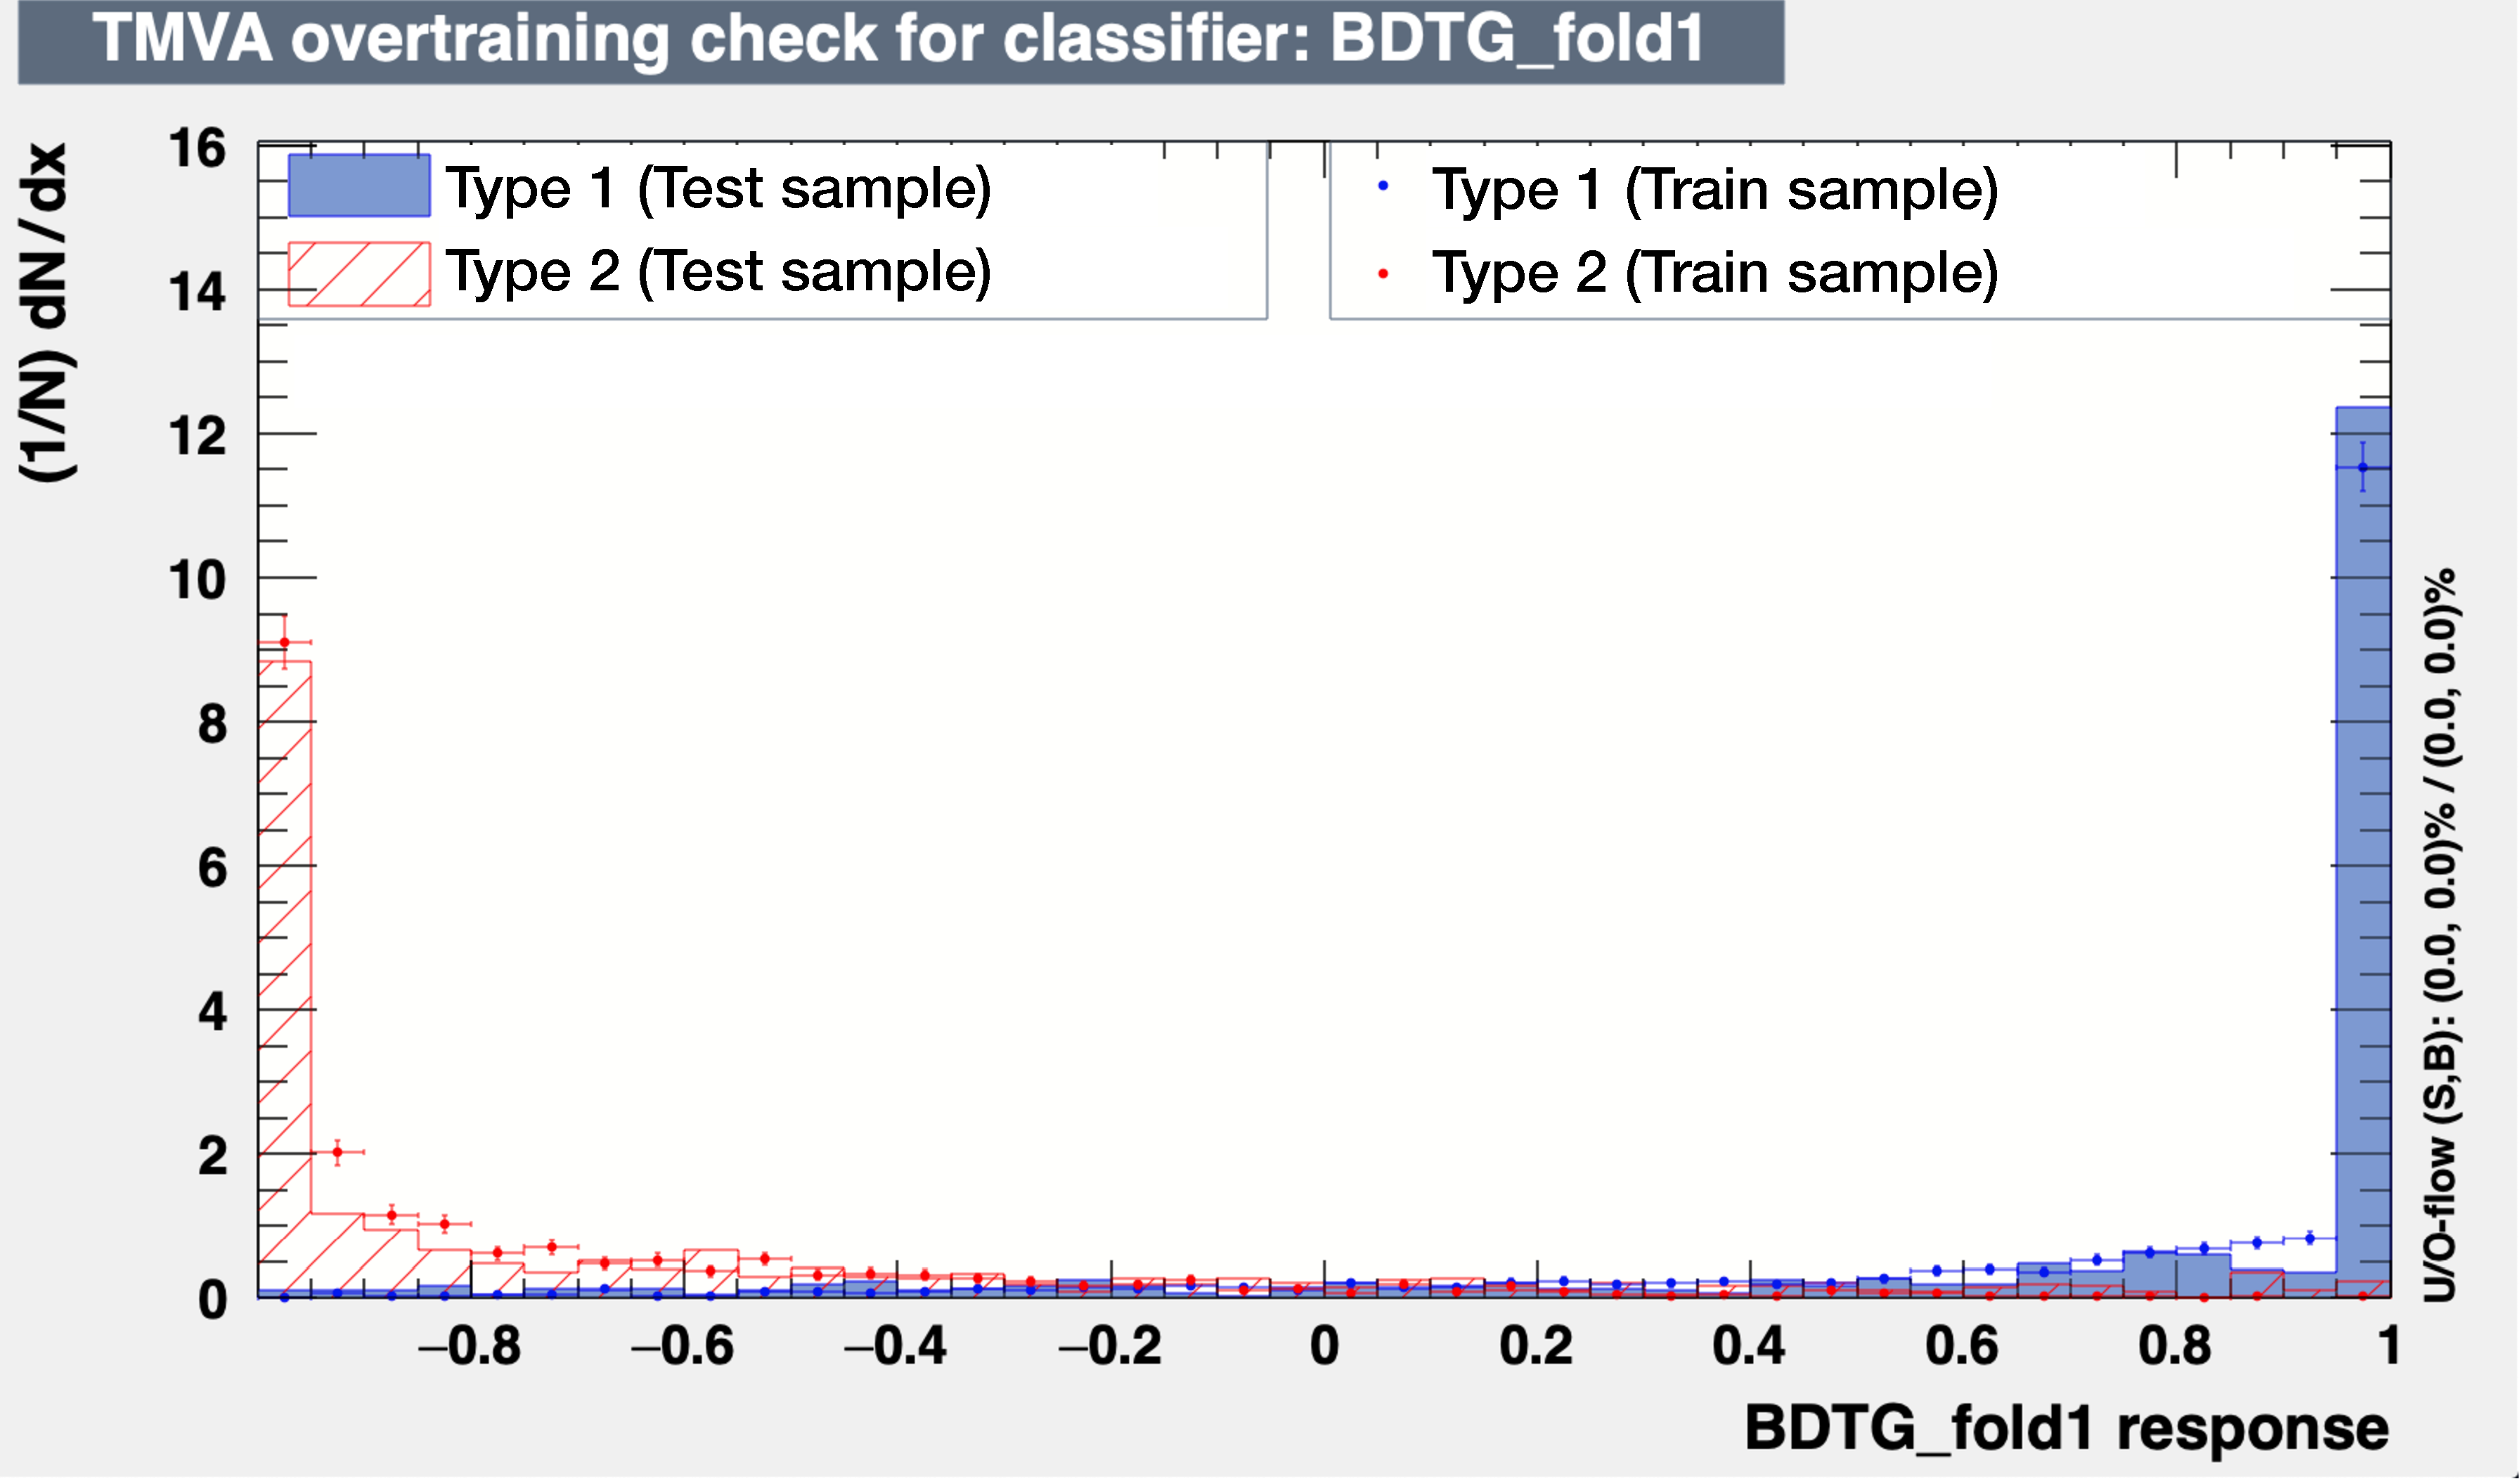
\includegraphics[width=.45\textwidth]{Chapter5_tHq/LeptAssociation/Dileptau_BDT_Based_Assignment_Score_Fold1}\quad
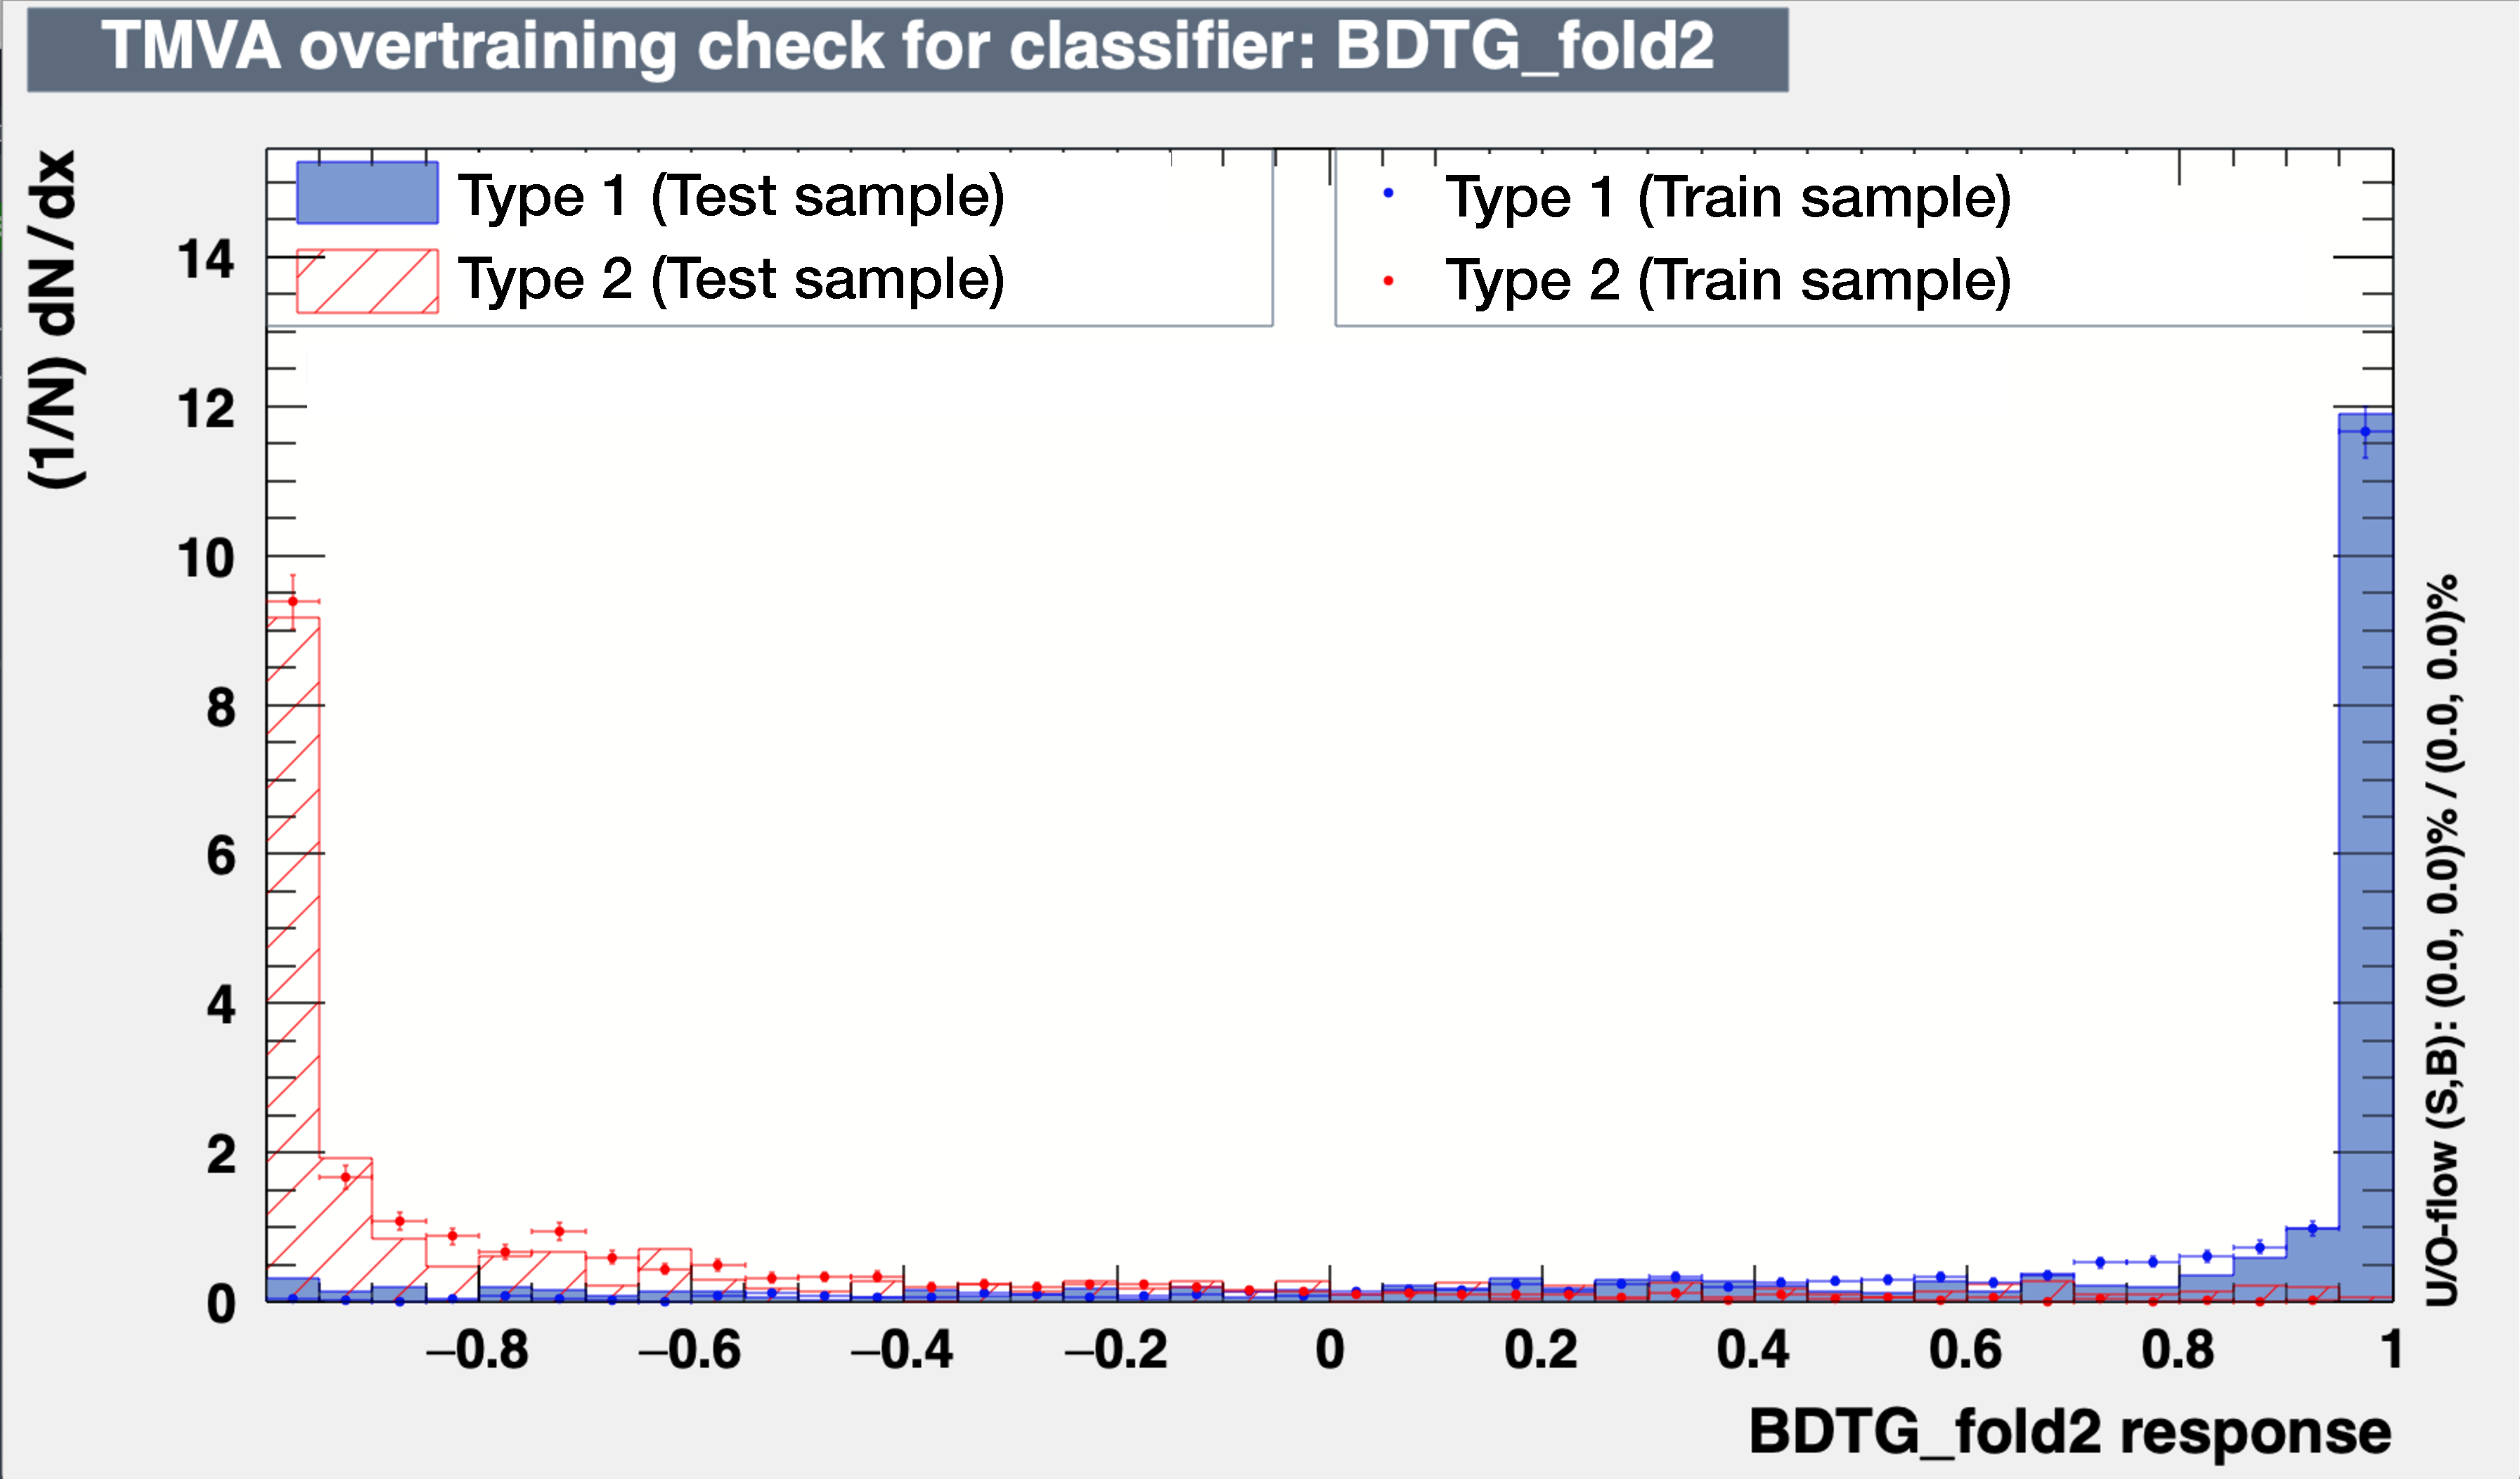
\includegraphics[width=.45\textwidth]{Chapter5_tHq/LeptAssociation/Dileptau_BDT_Based_Assignment_Score_Fold2}
\medskip
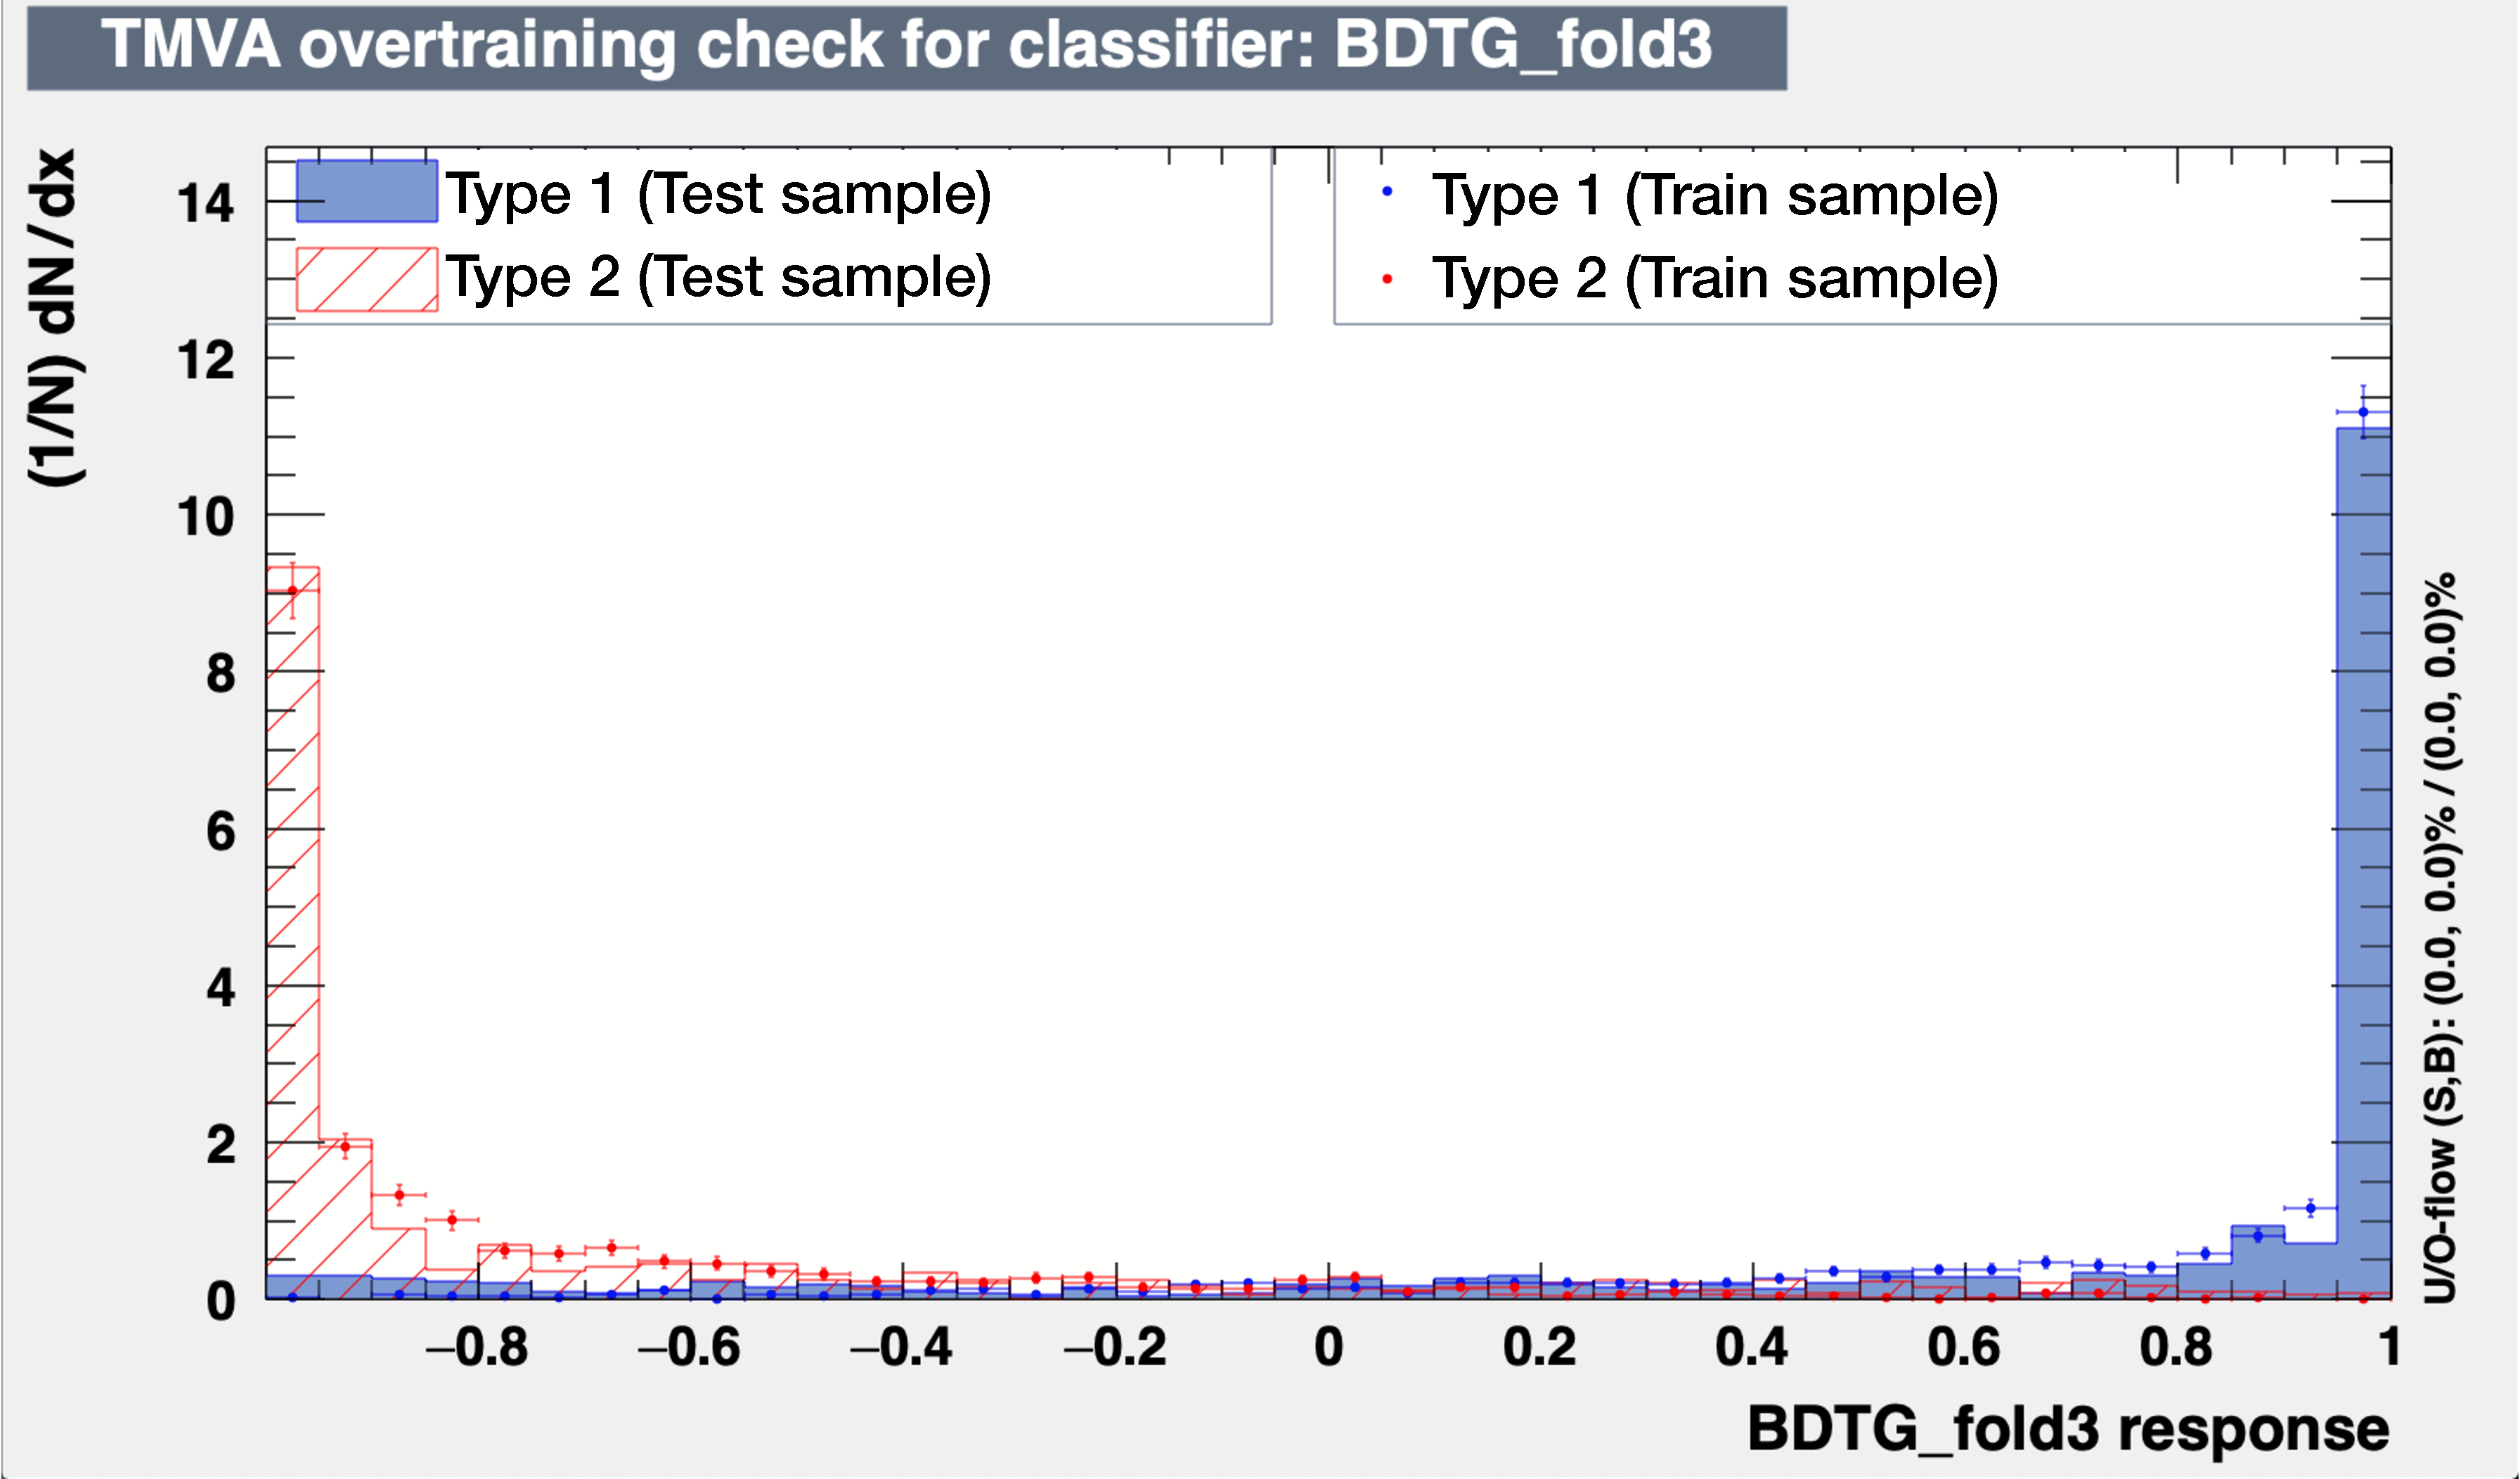
\includegraphics[width=.45\textwidth]{Chapter5_tHq/LeptAssociation/Dileptau_BDT_Based_Assignment_Score_Fold3}\quad

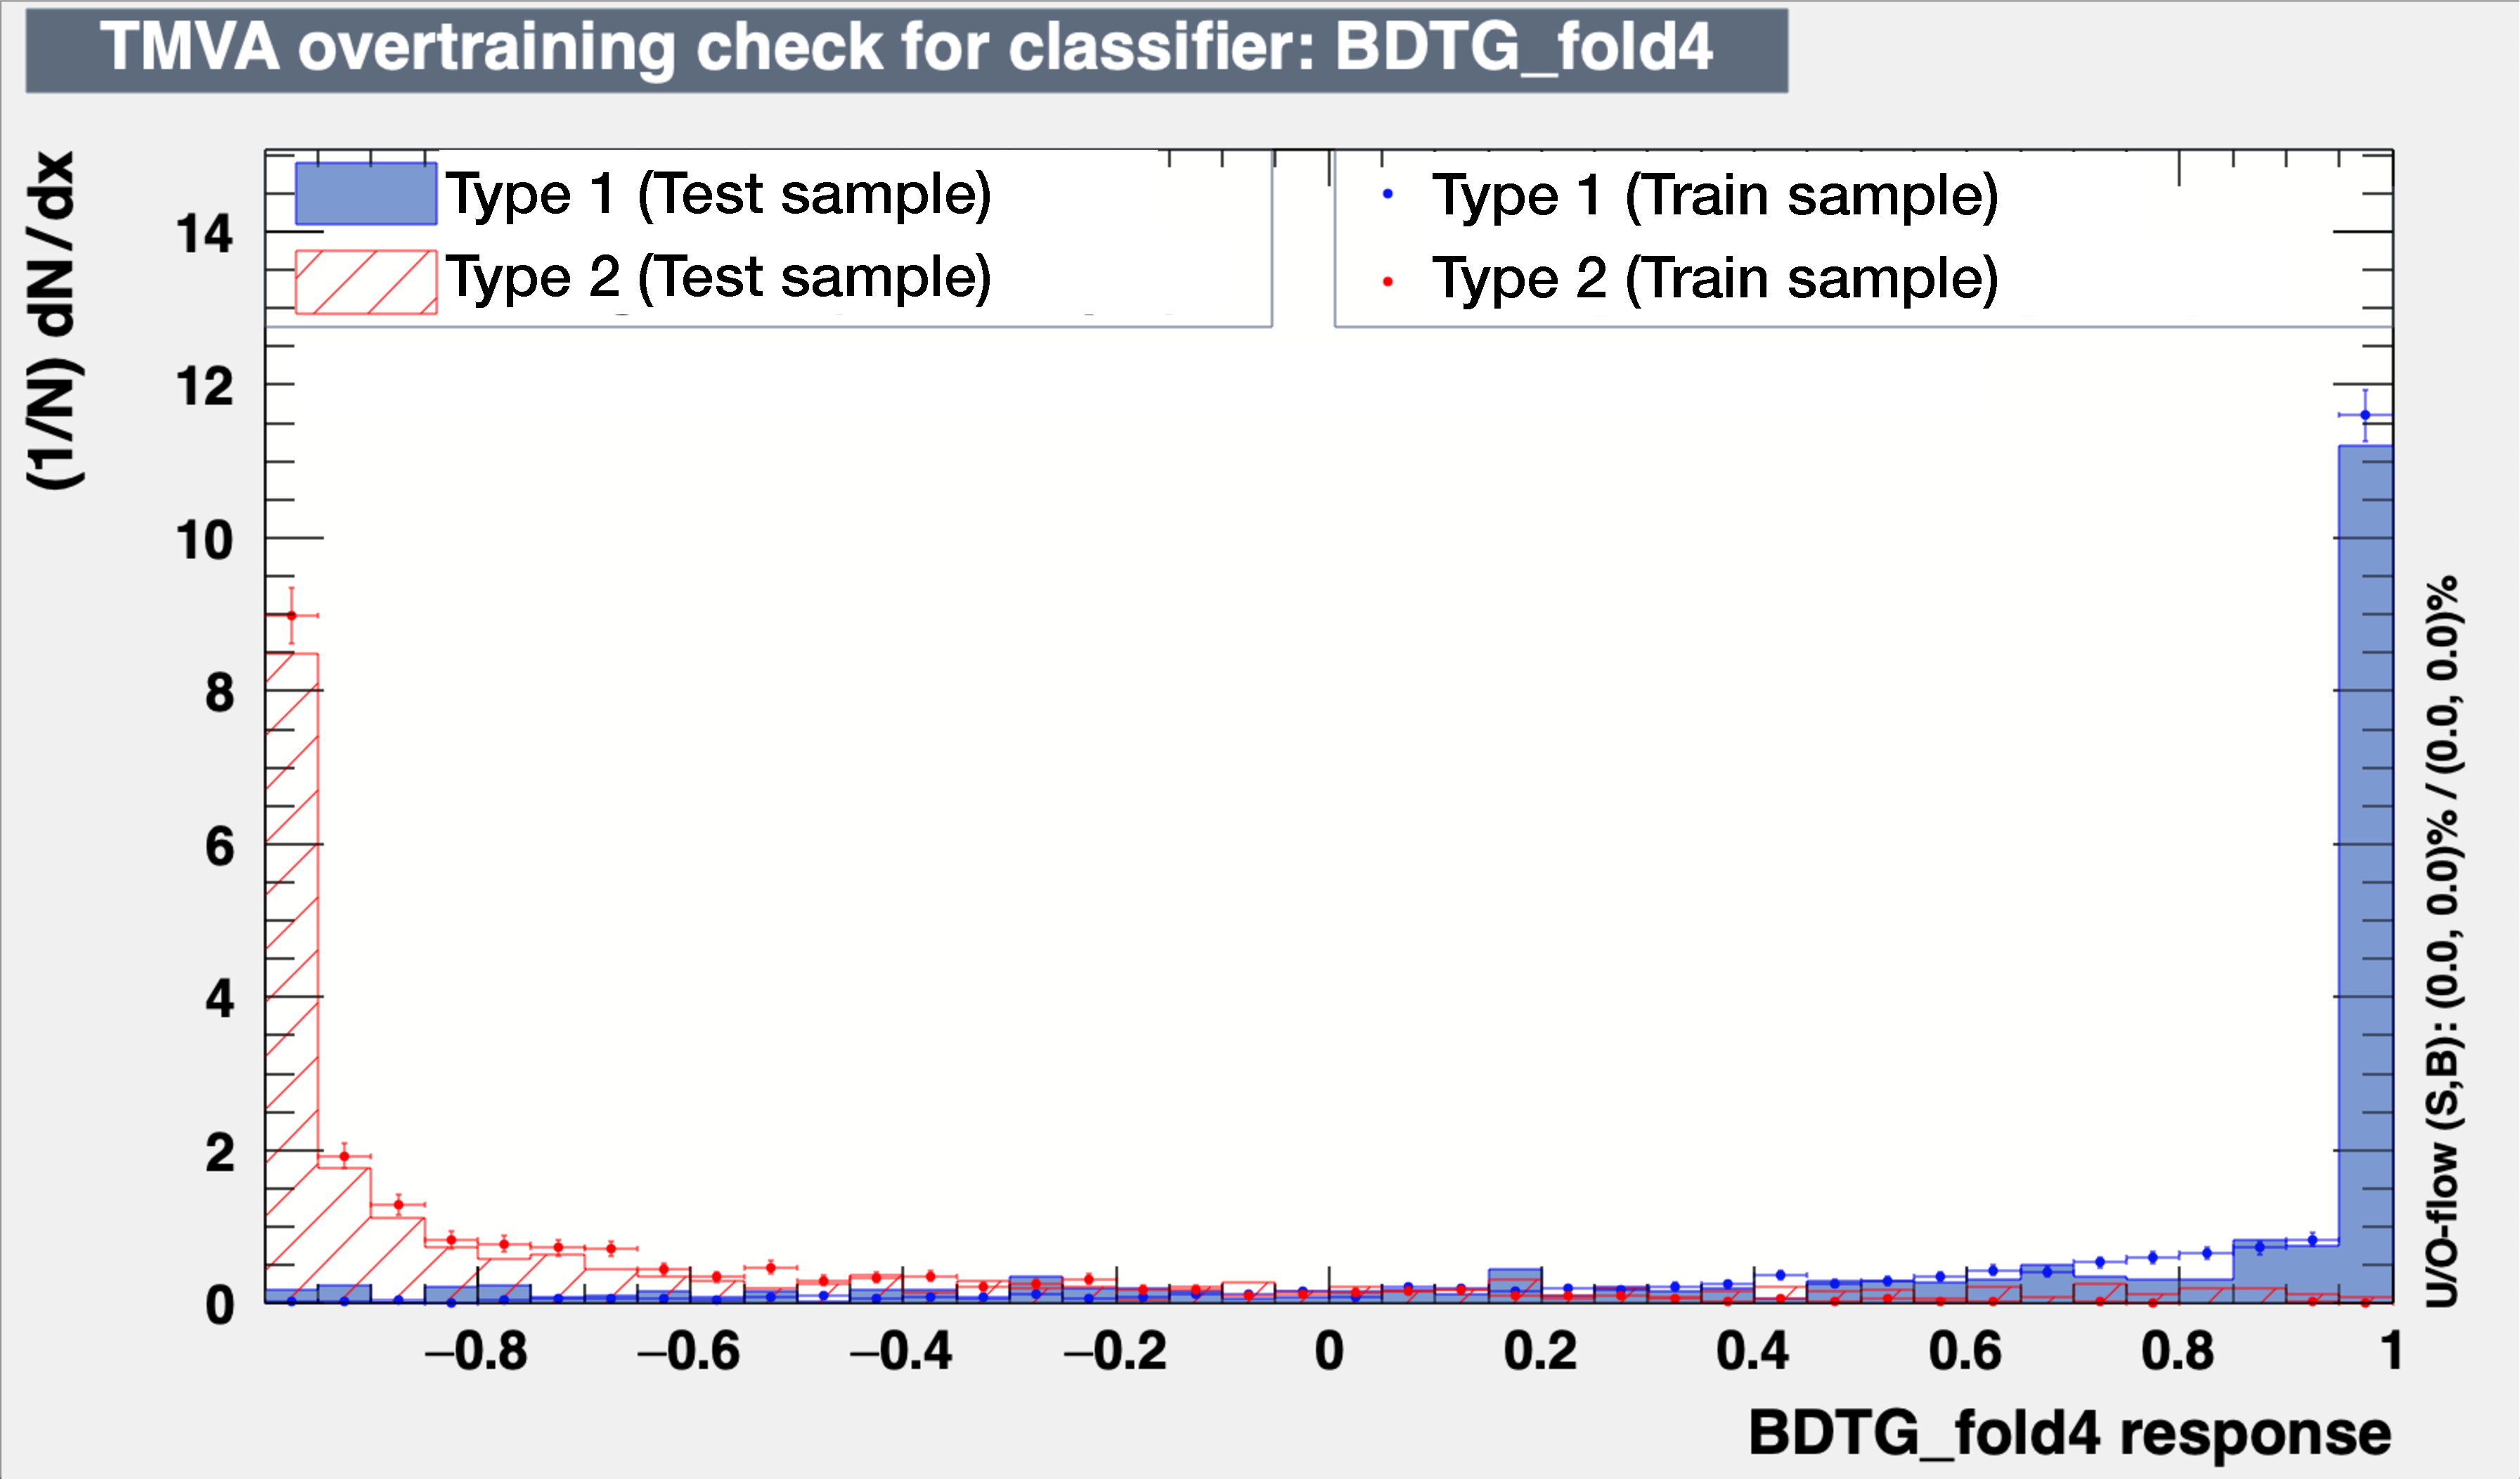
\includegraphics[width=.45\textwidth]{Chapter5_tHq/LeptAssociation//Dileptau_BDT_Based_Assignment_Score_Fold4}
\medskip
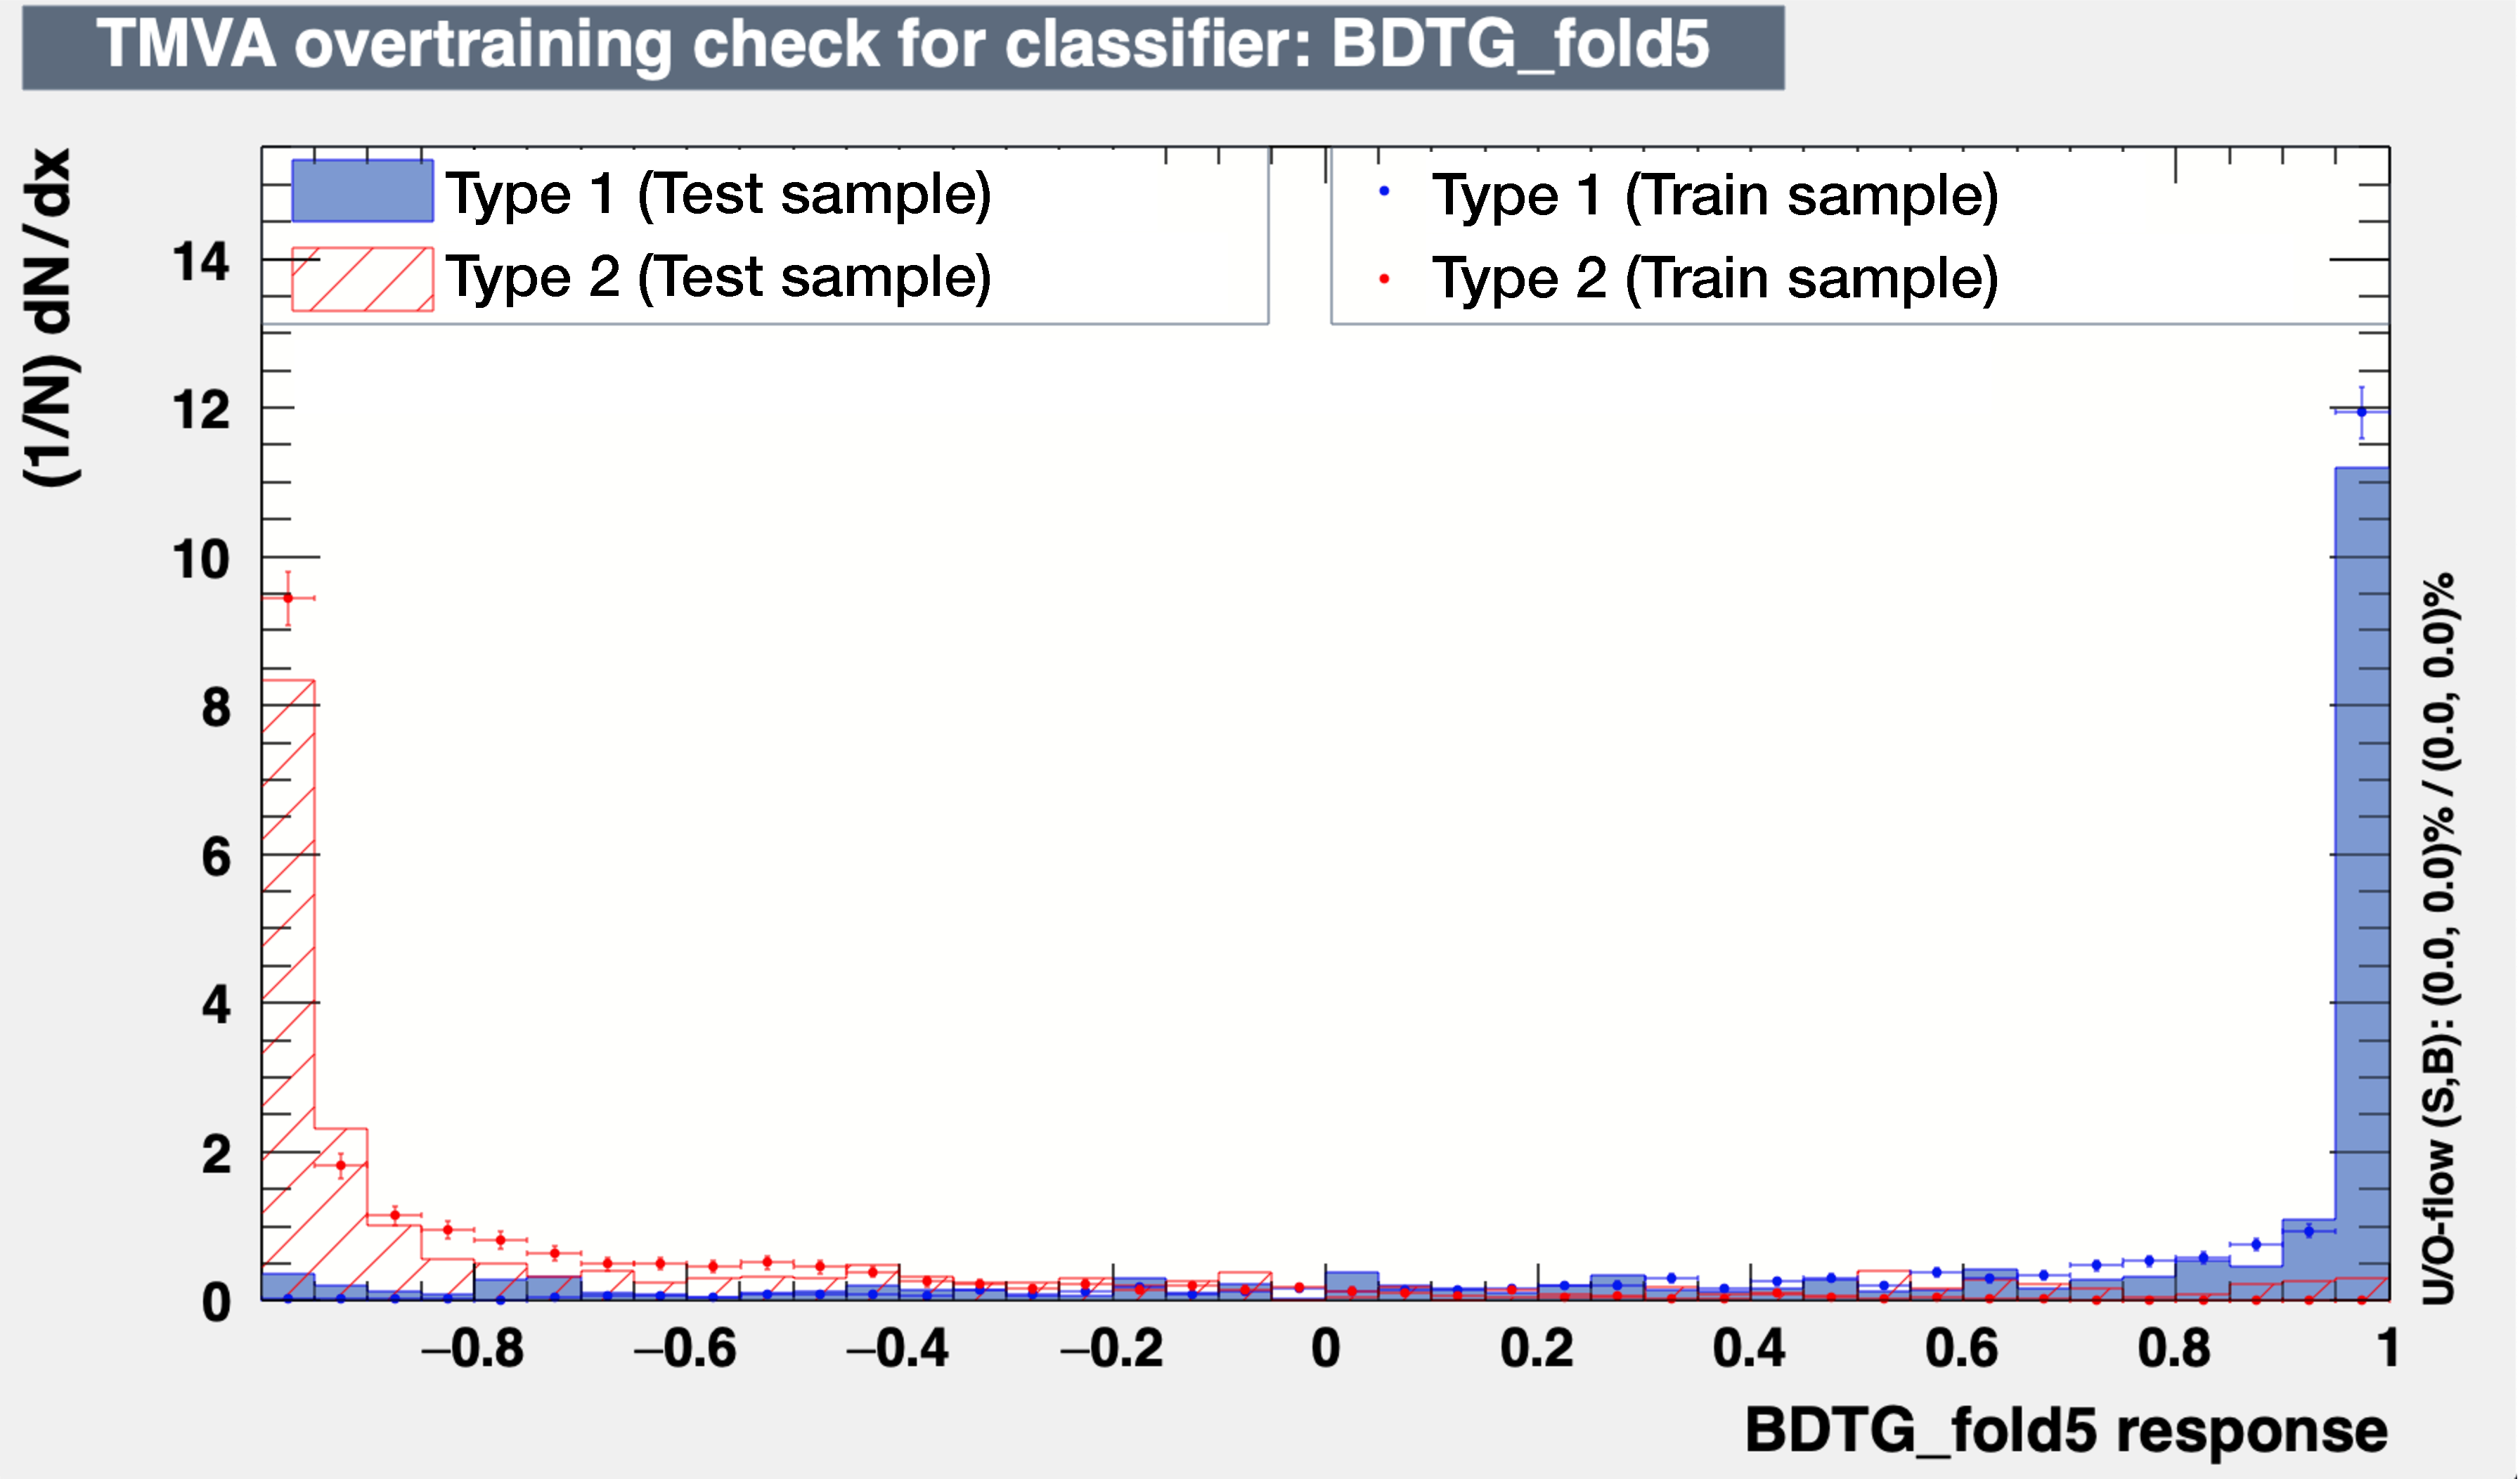
\includegraphics[width=.45\textwidth]{Chapter5_tHq/LeptAssociation/Dileptau_BDT_Based_Assignment_Score_Fold5}
\caption{BDT score distributions for the different models. The train and test samples 
are superimposed, allowing to check for overtraining.}
\label{fig:dileptau:Assignment_appendix:ScoreDistributions}
\end{figure}



Figures \ref{fig:dileptau:Assignment:ROC_and_Score:ROC} and 
\ref{fig:dileptau:Assignment:ROC_and_Score:Score} present the 
ROC curve and BDT score, respectively, separated by categories and 
combining the data from all five folds. The ROC curve illustrates the 
balance between correctly identifying Type$\,$1 instances and misclassifying 
Type$\,$2 instances at various classification thresholds. A higher ROC 
curve and a larger area under the curve (AUC) indicate improved 
classification performance. A more comprehensive explanation of these 
concepts can be found in Appendix \ref{chap:Appendix:BDT:Concepts}. 
Notably, the Type$\,$1 and Type$\,$2 categories replace the conventional 
positive and negative instances. The substantial AUC observed in the ROC 
curve signifies strong performance. For a detailed view of the ROC curves for
each fold individually, refer to Figure \ref{fig:dileptau:Assignment_appendix:ROCs}
in the appendix.

Regarding the BDT score in Figure \ref{fig:dileptau:Assignment:ROC_and_Score:Score}, 
it is evident that the Type$,$1 and Type$,$2 categories exhibit distinct peaks at opposite 
extremes of the distribution. This significant separation confirms the effectiveness of the 
BDT when differentiating between the two categories. It is worth noting that the bullets 
representing the train sample and the shadowed area representing the test samples 
appear identical due to the way TMVA combines the folds in a single histogram. 
However, the accurate assessment of the test versus train comparison is shown in Figure \ref{fig:dileptau:Assignment_appendix:ScoreDistributions}.

\begin{figure}[htbp!]
  \begin{subfigure}[h]{0.4\linewidth}
  	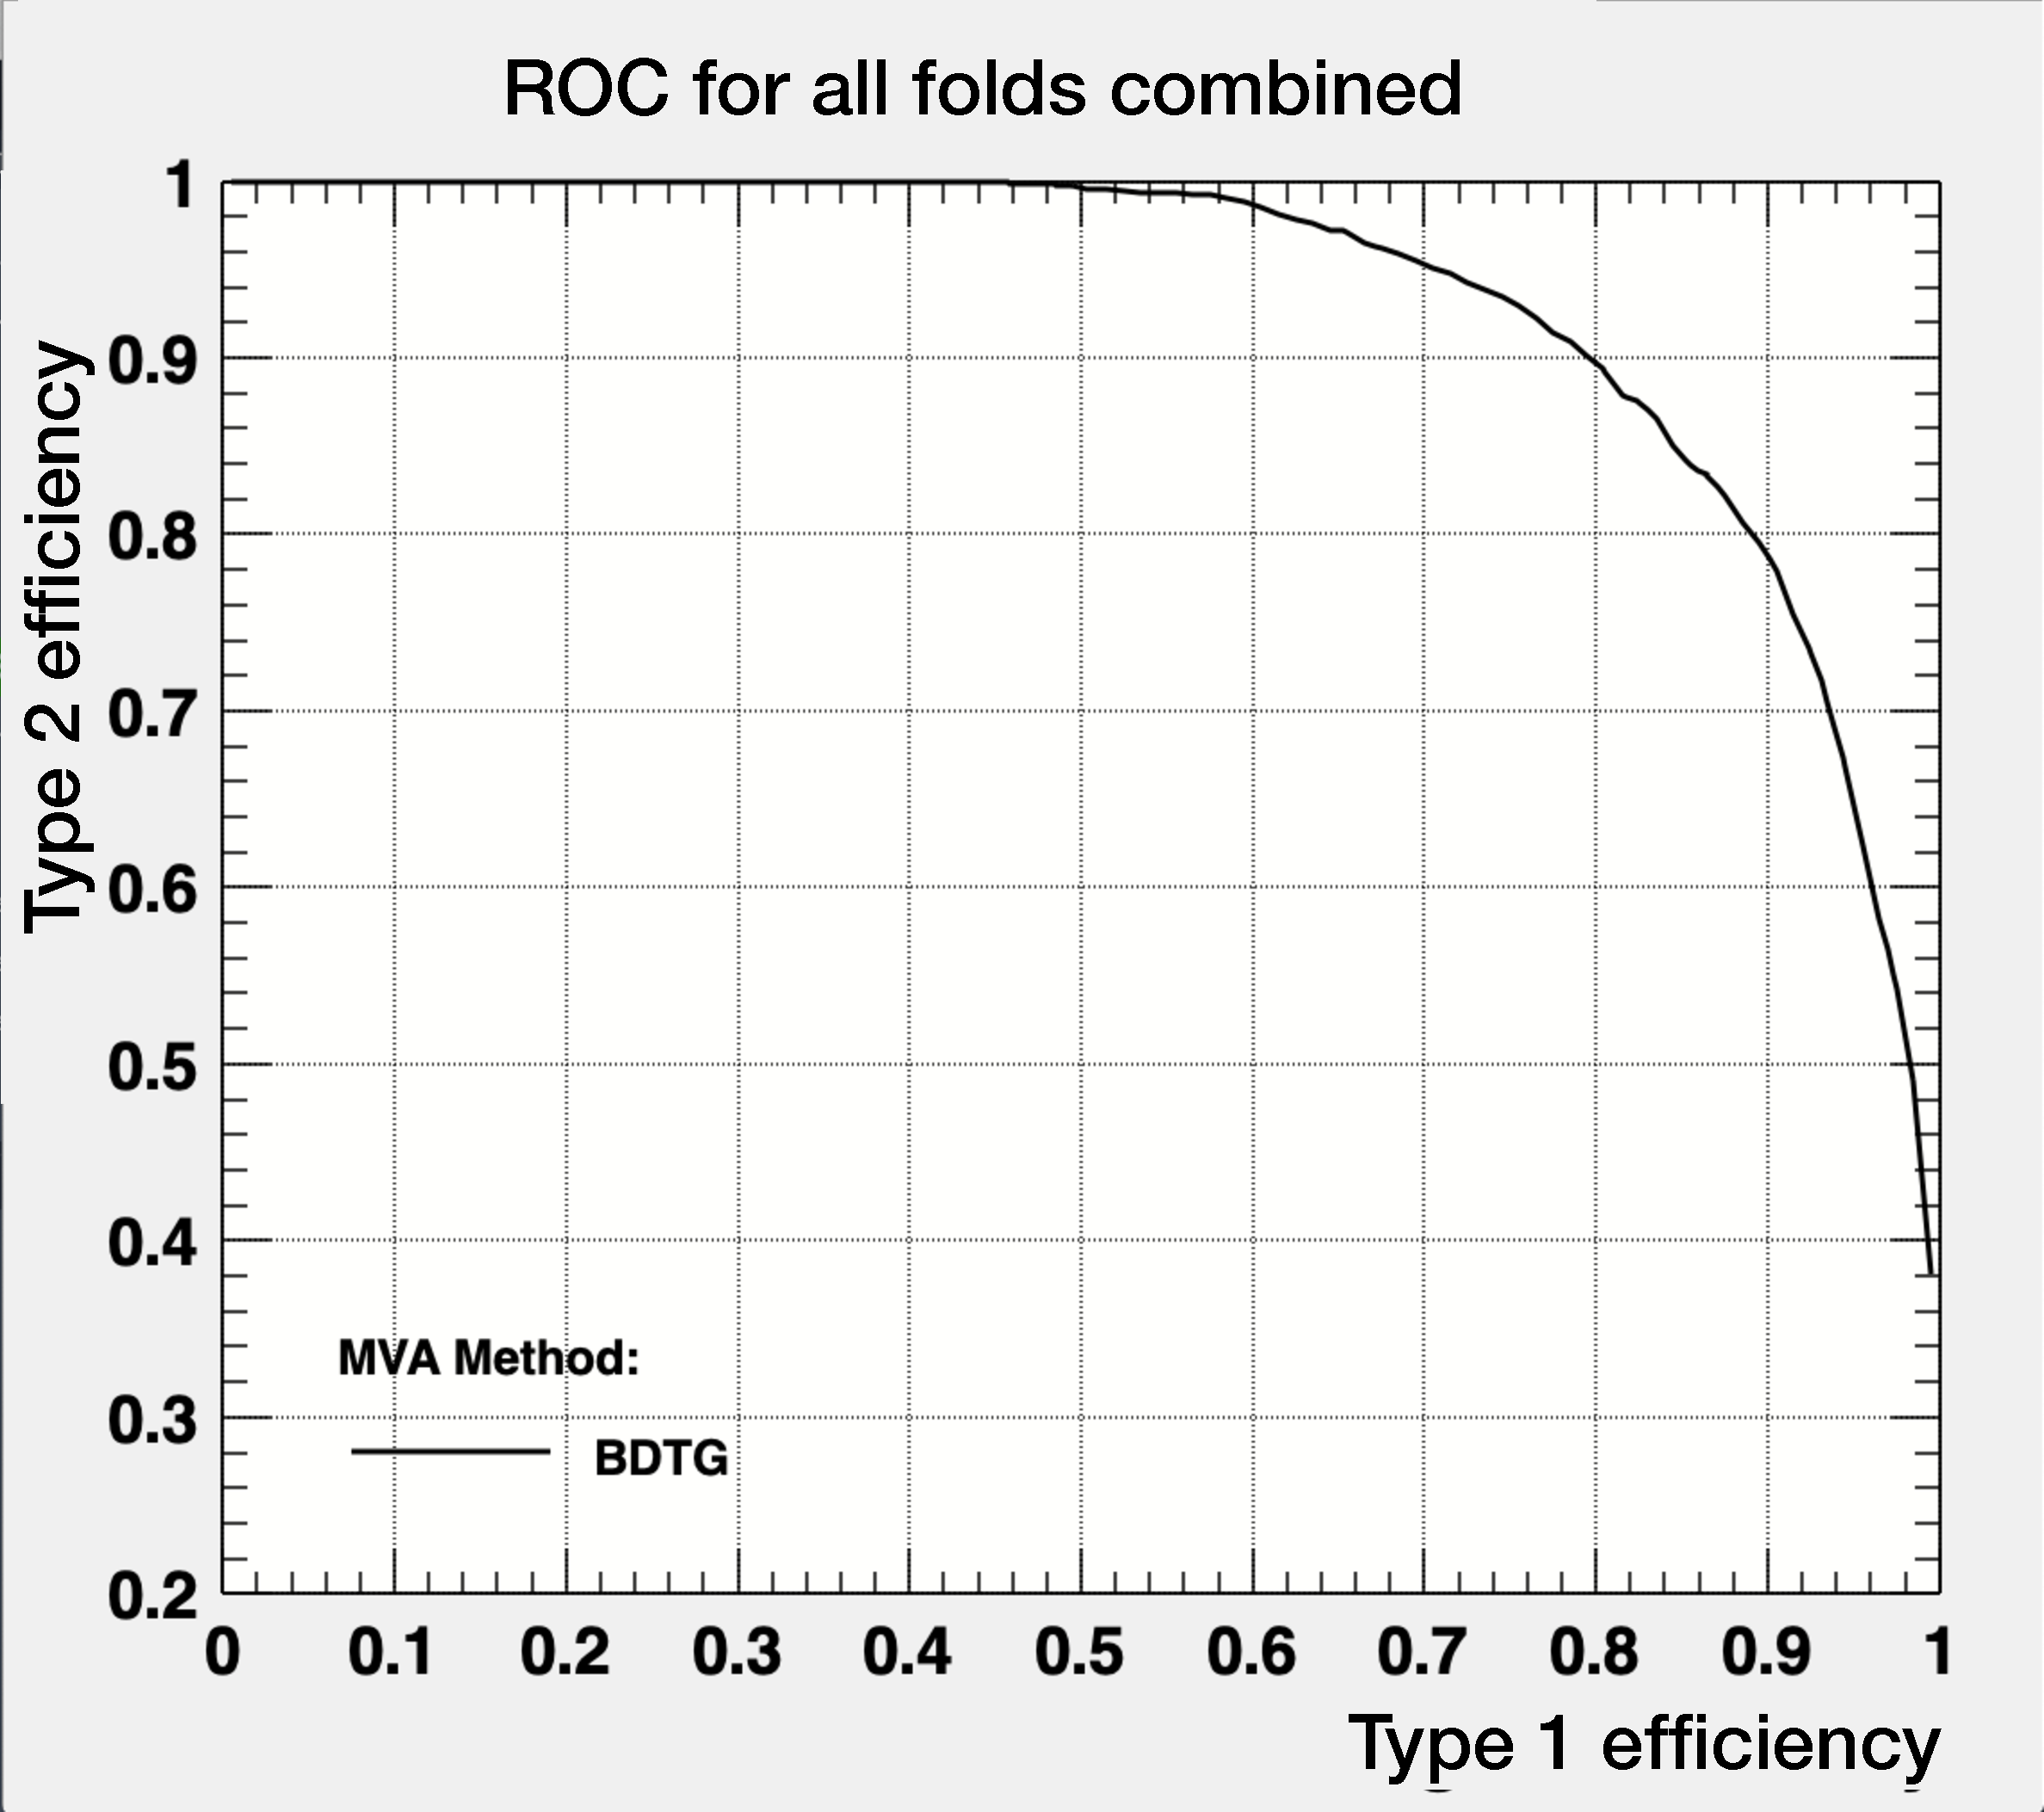
\includegraphics[width=\linewidth]{Chapter5_tHq/LeptAssociation/dileptau_ROC_Curve_General}
	\caption{ROC curve}
	\label{fig:dileptau:Assignment:ROC_and_Score:ROC}
  \end{subfigure}
  %\hfill
  \begin{subfigure}[h]{0.6\linewidth}
	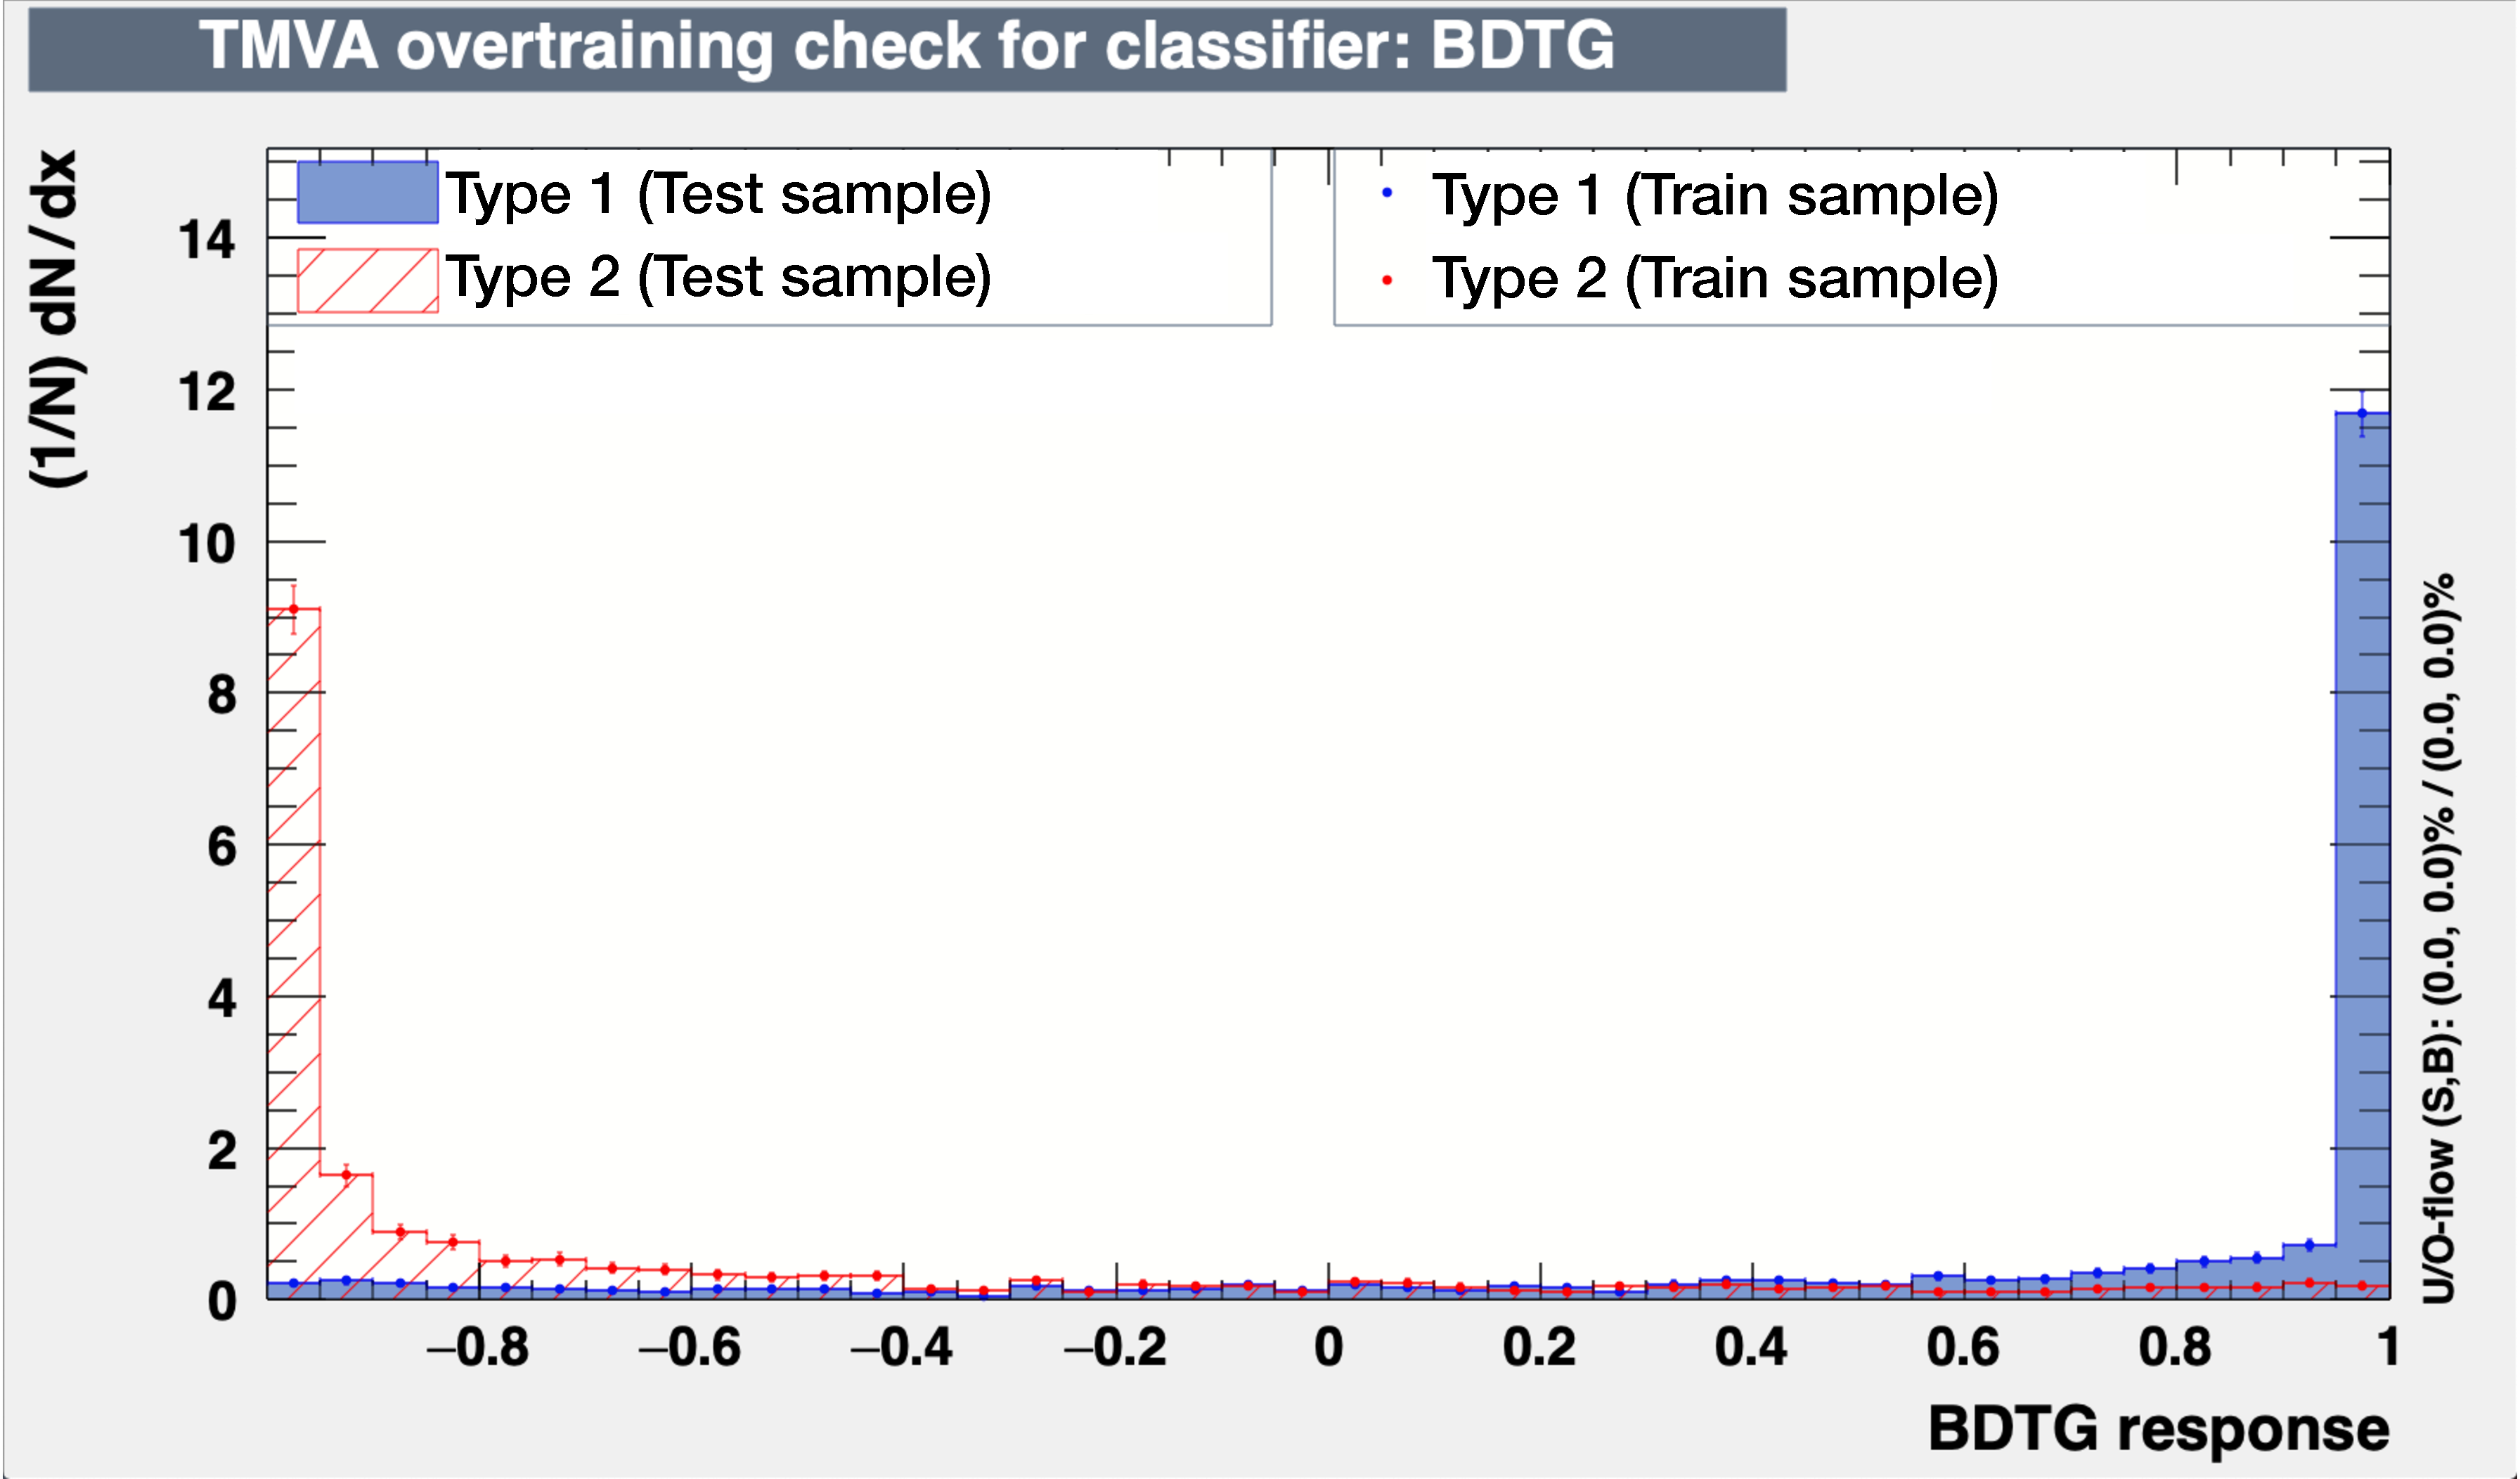
\includegraphics[width=\linewidth]{Chapter5_tHq/LeptAssociation/Dileptau_BDT_Based_Assignment_Score_General}
	\caption{BDT score} 
	\label{fig:dileptau:Assignment:ROC_and_Score:Score}
  \end{subfigure}%
\caption{ROC and score combining all folds for the \dilepSStau lepton-assignment BDT.}
\label{fig:dileptau:Assignment:ROC_and_Score}
\end{figure}
		 

\pablo{Faltan los plots (si existiesen, que no existen) de la logloss.}

 %%%%%%%%%%%%%%%%%%
%           BDT-Thereshold     %
%%%%%%%%%%%%%%%%%%
\subsubsection{Model application and classification threshold selection}
\label{sec:ChaptH:Sig:LepAsign:SS:BDT:Application}


Although the model building tool was initially developed as an independent 
and self-contained application, the BDT for assigning the origin of the light 
lepton is integrated into the \thqloop framework. As a result, during the production 
of post-processed NTuples (i.e. the \thqloop output), the lepton origin in the 
\dilepSStau is already used for variable construction. It is important to note 
that this procedure differs from the approach employed in the BDT for region 
definition discussed in Section \ref{sec:ChaptH:EventSelection}. In the latter BDT, 
the scores are injected separately within a distinct framework.

\begin{table}[]
\centering
\resizebox{\textwidth}{!}{
\begin{tabular}{l|lllllllll}
\toprule
BDT point     & -0.45 & -0.4  & -0.35 & -0.33 & -0.32 & -0.315 & -0.31 & -0.395 & -0.3  \\ \midrule
Accuracy (\%) & 88.12 & 88.03 & 87.97 & 88.23 & 88.33 & 88.39  & 88.36 & 88.32  & 88.15 \\ \bottomrule
\end{tabular}}
\caption{Different thresholds for lepton association compared to its correspondent accuracy.}
\label{tab:dileptau:Assignment_appendix:Thereshold}
\end{table}


 %%%%%%%%%%%%%%%%%%
%           BDT-Results    %
%%%%%%%%%%%%%%%%%%
\subsubsection{Results of the BDT-based method for lepton assignment}
\label{sec:ChaptH:Sig:LepAsign:SS:BDT:Results}


The result obtained by this method can be compared to the one given by the cut-based alternative method 
described in at the beginning of this Section. A summary of the performance of the two methods
is given in Table \ref{tab:dileptau:Assignment:MethodsSummary}.

\begin{table}[]
\centering
\begin{tabular}{l|lll|}
\cline{2-4}
 & \multicolumn{3}{c|}{Accuracy} \\ \cline{2-4} 
                                       & \multicolumn{1}{l|}{Total (100\%)} & \multicolumn{1}{l|}{$H\rightarrow \tau \tau$ (83.08\%)} & $H\rightarrow WW$ (16.92\%) \\ \hline
\multicolumn{1}{|l|}{BDT-based method} & \multicolumn{1}{l|}{88,39}         & \multicolumn{1}{l|}{88.44}             & 88.18         \\ \hline
\multicolumn{1}{|l|}{Cut-based method}       & \multicolumn{1}{l|}{83.86}         & \multicolumn{1}{l|}{84.24}             & 81.80         \\ \hline
\end{tabular}
\caption{Accuracy calculated by comparing the prediction of the method to the true value. 
The true value has been obtained using the labelling described in Section \ref{sec:tHq:origin:LeptonAssignment_truth_reco_DeltaRCone}. 
This labelling is only available for \Htautau and \HWW. Only events with successful truth-reco matching have been used info produce the table.
From the events with successful truth-reco matching, 83\% are \Htautau and 17\% \HWW.}
\label{tab:dileptau:Assignment:MethodsSummary}
\end{table}




 
 
\subsubsection{Las movidas que no quiero olvidar decir}
\begin{itemize}
	\item Compare to the results using other MVA methods.
	\item The BDT is integrated in \thqloop (weights.xml) ¿Where do I describe what \thqloop is?
	\item From \thqloop, the BTD score can be calculated for all the events (signal or not) and then 
	the efficiency of the lepton association can be calculated depending on the threshold point which is
	chosen to define whether the event is Type$\,$1 or Type$\,$2. Note that this efficiency is computed only over
	signal events. $\rightarrow$ Table of 'efficiency vs cutpoint'
	
	\item \textbf{Result}: 
		\begin{itemize}
			\item ROC curves for all folds in Figure \ref{fig:dileptau:Assignment_appendix:ROCs}
			\item Table \ref{tab:dileptau:Assignment_appendix:Thereshold} is exploring classification 
			accuracies depending on which BDT-score point is used to separate type1 and type 2.	
		\end{itemize}
\end{itemize}



%%%%%%%%%%%%%%%%%%%%%%%%%%%%
%           Top quark and Higgs boson reconstruction      %
%%%%%%%%%%%%%%%%%%%%%%%%%%%%
\subsection{Top quark and Higgs boson reconstruction}
\label{sec:ChaptH:Sig:EventReconstruction} 
% Source: Presentation on 14/10/2020
%.              https://www.overleaf.com/project/5f74653051c93a00018b5f95
In order to suppress background, it is desirable to reconstruct the 
kinematics of both the top quark and the Higgs boson. 
By doing this, it is possible to define variables that can further separate the signal.
However, the accurate reconstruction of these particles is a challenging task 
due to the presence of four neutrinos in the final state, of which at least three 
are from the Higgs boson and one is from the top quark\footnote{This is 
assuming the most common decay channel, \Htautau.}. 
In this work, the strategy used to fully reconstruct the top and the Higgs consists on first
reconstructing the top-quark system and then the Higgs-boson chain. Since we know
the total \MET, if the missing energy is reconstructed for the top quark, 
it is possible to access the $\overrightarrow{E}_{\text{T}}^{\text{miss}} (\text{Higgs})$ based on:
\begin{equation*}
	\overrightarrow{E}_{\text{T}}^{\text{miss}} (\text{total}) = \overrightarrow{E}_{\text{T}}^{\text{miss}} (\text{Higgs}) + \overrightarrow{E}_{\text{T}}^{\text{miss}} (\text{top}) \,.
\end{equation*}

In the escenario in which the Higgs decays to $\Ptauon \APtauon$, all possible 
decay configurations are described in Table \ref{tab:ChaptH:Reconstuction:Configurations}.
From this table, the first two jet columns represent 92.7\% of \Htautau events 
while the last one can be neglected. This has been calculated from the numbers in Table \ref{tab:ChaptH:TruthSummary}.
This two columns represent the scenario in which the \tauhad comes from the  \PHiggs.
This particular decay form of the  \tHq(\dileptau) production is presented in the Feynman diagram of
Figure \ref{fig:tHq:TruthFeyman}. 


\begin{table}[]
\centering
\begin{tabular}{l|l|l|l|l}
\toprule
 $q$ & $q$ & jet & jet & jet \\ \midrule
 $H$ & $\tau$ & $\tauhad \: \nu_{\tau}$           &  $\tauhad \: \nu_{\tau}$           & $\Plepton_1 \: \nu_{\Plepton_1} \: \nu_{\tau}$ \\ 
     & $\tau$ & $\Plepton_1 \: \nu_{\Plepton_1} \: \nu_{\tau}$ &  $\Plepton_2 \: \nu_{\Plepton_2} \: \nu_{\tau}$ & $\Plepton_2 \: \nu_{\Plepton_2} \: \nu_{\tau}$ \\ \midrule
 $t$ &  $W$   & $\Plepton_2 \: \nu_{\Plepton_2}$               &  $\Plepton_1 \: \nu_{\Plepton_1}$               &  $\tauhad \: \nu_{\tau}$          \\ %\hline
     &  $b$   &  $b$-jet                         &  $b$-jet                          & $b$-jet                          \\ \bottomrule
\end{tabular}
\caption{Possible configurations of the final state objects in the \dileptau channel when the Higgs decays
to \tauhad and \taulep. The first column presents the spectator quark $q$, the \PHiggs boson and the \Ptop quark.
The second column shows the \PHiggs and \Ptop decays. The other three columns show the different possible configurations in 
which these objects can further decay.}
\label{tab:ChaptH:Reconstuction:Configurations}
\end{table}


\begin{figure}[htbp!]
\centering
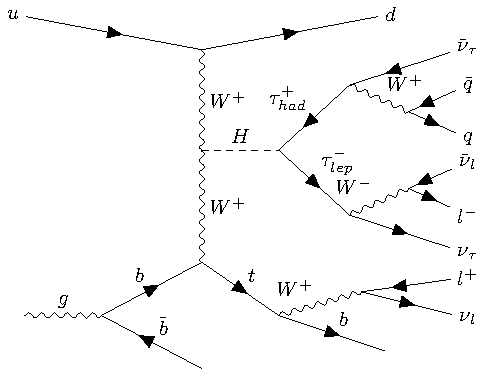
\includegraphics[width=.75\textwidth]{Feynman_diagrams/Feynman_DileptauGeneralRepresentative_dileptau_OS}
\caption{Representative LO Feynman diagram for the \tHq (\dileptau) in the $\PHiggs \rightarrow \tauhad \taulep$ decay channel. 
\pablo{Esta figura ya la pones en la intro del capítulo}}
\label{fig:tHq:TruthFeyman}
\end{figure}

Before reconstructing the top quark or Higgs boson, the two charged-light leptons in the final state have to be
assigned to its correspondent parent. In most of cases, one $\Plepton$ comes from the Higss and the other 
from the top. The origin association is described with detail in Section \ref{sec:ChaptH:Sig:LepAsign}.

%% Top quark reconstruction %%
\subsubsection{Top quark reconstruction}
In order to reconstruct the top quark, it is essential to have complete knowledge of the 4-momentum of both 
the $\PW$ boson and the $\Pbottom$ quark. However, the reconstruction of the $\PW$ boson decay presents a 
significant challenge due to the kinematics of the neutrino, which escapes the detector without being detected.
Therefore, if we are able to reconstruct the neutrino, the top system can be reconstructed as well. 

The objective is to obtain the \MET of the top-quark system ($\overrightarrow{E}_{\text{T}}^{\text{miss}} (\text{top})$), 
for which it is sufficient\footnote{Determining $p^{z}_{\Pnu}$ would add a constrain and, hence, it would be 
possible to get exact solutions for al the components of $\overrightarrow{p}_{\Pnu}$.}
 to determine the z-component of the neutrino momentum ($p^{z}_{\Pnu}$). 
In order to achieve this, various hypotheses have been examined using truth-level information. 
One of the initial hypotheses tested was whether the z-component of the neutrino momentum in the top-quark system 
exhibits a linear dependence with a coefficient $\alpha$ on the z-component of the momentum of the light lepton. 

\begin{figure}  
	\begin{subfigure}{0.45\textwidth}
	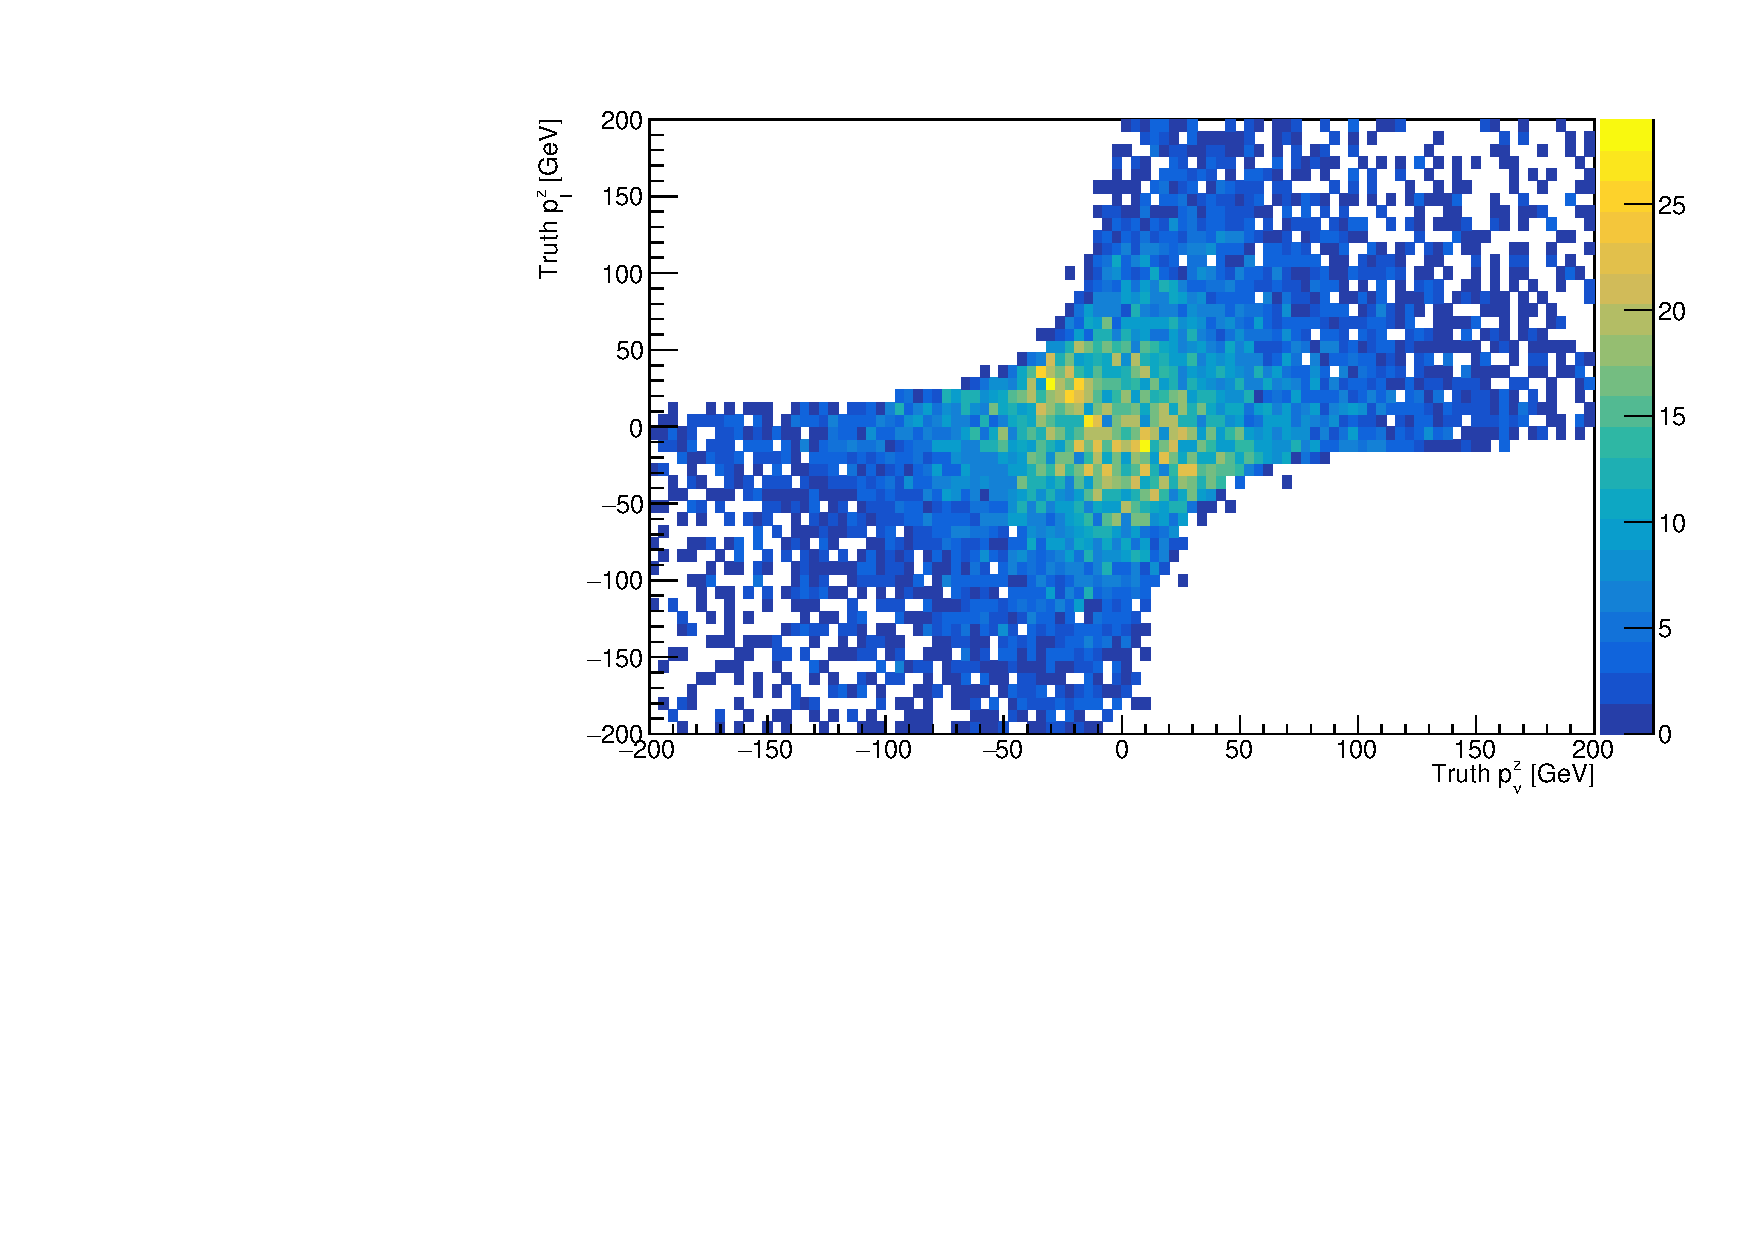
\includegraphics[width=\linewidth]{Chapter5_tHq/Reconstruction/Pzv_vs_Pzl_truth_alp05}
	\caption{Truth $p^z_l$ vs. Truth $p^z_\nu$}
	\label{fig:tHq:EventReconstruction:TopSystem:hypothesis1:A}
	\end{subfigure}
\hfill 
	\begin{subfigure}{0.45\textwidth}
	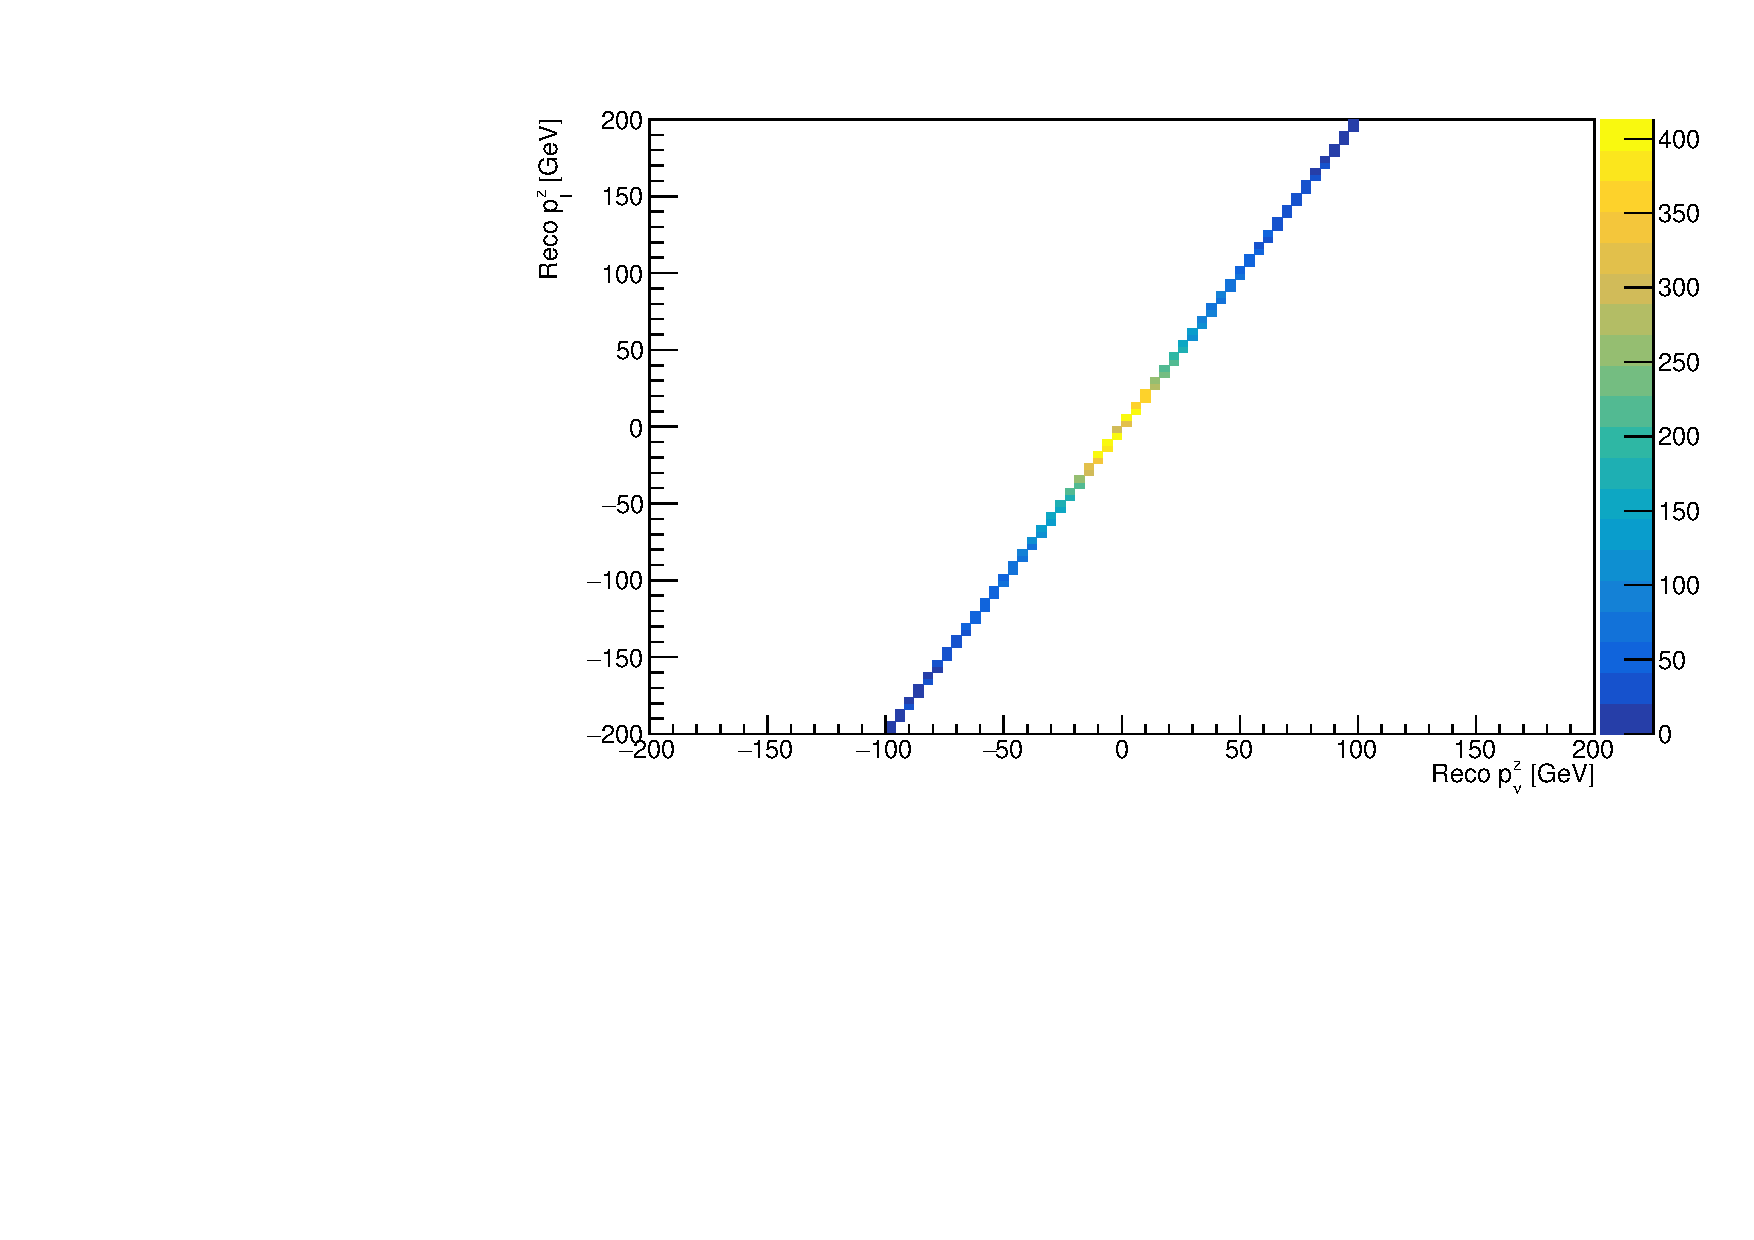
\includegraphics[width=\linewidth]{Chapter5_tHq/Reconstruction/Pzv_vs_Pzl_Reco_alp05}
	\caption{Reco. $p^z_l$ vs. Reco. $p^z_\nu$}
	\label{fig:tHq:EventReconstruction:TopSystem:hypothesis1:B	}
	\end{subfigure}

\bigskip  
	\begin{subfigure}{0.45\textwidth}
	\includegraphics[width=\linewidth]{Chapter5_tHq/Reconstruction/truth_vs_reco_pz_l_alp05}
	\caption{Reco. $p^z_l$ vs. Truth $p^z_l$}
	\label{fig:tHq:EventReconstruction:TopSystem:hypothesis1:C}
	\end{subfigure}
\hfill 
	\begin{subfigure}{0.45\textwidth}
	\includegraphics[width=\linewidth]{Chapter5_tHq/Reconstruction/truth_vs_reco_pz_nu_alp05}
	\caption{Reco. $p^z_\nu$ vs Truth $p^z_\nu$}
	\label{fig:tHq:EventReconstruction:TopSystem:hypothesis1:D}
	\end{subfigure}

\caption{Distributions comparing $p^{z}_{\Pnu}$ and $p^{z}_{\Plepton}$
at truth and reconstruction levels for \tHq \dileptau events.} % Overall figure caption
\label{fig:tHq:EventReconstruction:TopSystem:hypothesis1}
\end{figure}

The parameter $\alpha$ represents a real number ranging from -1 (indicating a back-to-back topology between 
the neutrino and the lepton) to 1. %For instance, $\alpha = 0$ would imply that the neutrino momentum was 
%parallel to the momentum of the lepton. 
The conducted studies have indicated that the hypothesis $p^{z}_{\Pnu} = \alpha \cdot p^{z}_{\Plepton}$ is not supported
as Figure \ref{fig:tHq:EventReconstruction:TopSystem:hypothesis1:A} shows. 


In order to reconstruct the kinematics of the top quark, another constrain had to be 
imposed on the neutrino. Through the correlation analysis between the neutrino and 
the top-quark lepton, the following constraints were defined:
\begin{align}
    \pnutopT & =\frac{1615.98\, \text{GeV}^2}{\pltopT}\,,\\
    \phinutop &= \philtop\pm\frac{\pi}{2}\, ,
\end{align}
where \phinutop and \philtop are, respectively, the azimuthal angles of the 
the neutrino and lepton from the leptonic decay of the top quark, and 
\pnutopT and \pltopT their transverse momentums. 

To resolve the sign ambiguity of the second constraint, the information regarding 
the \Pbottom-quark is considered. This involves imposing the following condition:
\begin{align*}
  \phibtop-\philtop \geq 0 & \rightarrow \phinutop=\philtop-\frac{\pi}{2}\,,\\
  \phibtop-\philtop < 0  & \rightarrow \phinutop=\philtop+\frac{\pi}{2}\, ,
\end{align*}
being \phibtop the azimuthal angle of the \Pbottom quark originated on the top-quark
decay.

The calculation of the reconstructed top-quark mass, \toprecomass, incorporates several 
variables, including the lepton associated with the top quark, the leading \bjet, and the 
neutrino \pnutopT and \phinutop. However, in this calculation, the $p^{z}_{\Pnu}$
component is set to zero do to its unknown value.

\subsubsection{Higgs boson reconstruction}
Mass reconstruction plays a crucial role in creating discriminating variables. 
A straightforward method for reconstructing the Higgs-boson mass involves 
summing its visible decay products. Assuming the \Htautau decay mode:
\begin{equation}
\Hvismass = \text{mass}(\Pgt_{\text{vis}, 1} + \Pgt_{\text{vis}, 2}) \, ,
\end{equation}
where  $\tauvis$ is either the visible part of the \tauhad
or the light lepton from the \taulep.

However, this approach overlooks the contribution of neutrinos and is therefore insufficient. 
By neglecting smaller contributions to the \MET, such as energy loss in detector material, 
it becomes possible to relate $\pT^{miss}(\PHiggs)$ to the measured \MET and the 
$\pT^{miss}(\Ptop)$ by imposing the relation:
\begin{equation*}
    p^{\text{miss}}_{x,y}(\PH) = p^{\text{miss}}_{x,y}(\text{measured})
      - p^{\text{miss}}_{x,y}(\text{top, reconstructed})\,.
\end{equation*}
The quantities \pnutopT and \phinutop, calculated in the previous section, are used in this relation.

This characteristic can be effectively employed in established methods for reconstructing 
the Higgs-boson mass. In the present analysis, the \MMC (Missing Mass Calculator) method, 
originally developed for the \Htautau analysis \cite{ELAGIN2011481}, is utilised.

\pablo{¿poner las figuras del Florian comparando los distintos métodos para reconstruir la masa?}

\pablo{¿poner una descripción del \MMC? Ver apéndice  "C.4.1.8 The description of the MMC method"  de la IntNote}

Alternatively, two other methods to reconstruct the \tautau system have been explored:
\begin{itemize}
	\item Method 1: Partial invariant mass
	\item Method 2: Collinear approximation
%source: https://www.overleaf.com/project/5f74653051c93a00018b5f95
\end{itemize}


%%%%%%%%%%%%%%%%%%%
%           Background estimation        %
%%%%%%%%%%%%%%%%%%%
\section{Background estimation}
\label{sec:ChaptH:Bkg}

\pablo{Explain what does it mean to estimate the backgrounds. For some process, such as the irreducible backgrounds, the MC simulations are good to estimate the yields. However, for other processes like the fake backgrounds this is not the case and here it comes Oleh's work which I shall describe}



%%%%%%%%%%%%%%%%
%     Reducible backgrounds  %
%%%%%%%%%%%%%%%%

\subsection{Reducible backgrounds}
\label{sec:ChaptH:Bkg:Fakes}
%\pablo{"Tools for estimating fake/non-prompt lepton bkgs" in reference \cite{ATLAS:2022swp}}
\url{https://arxiv.org/pdf/2211.16178.pdf}




\paragraph{Light-lepton fakes} % When talking about promt, non-prompt and fakes it is recomended to avoid the work real.

Particles from the hard scattering process are referred as `prompt'. 
Acceptance, quality and isolation requirements are applied to select these leptons
Non-prompt leptons and non-leptonic particles may satisfy these selection criteria, 
giving rise to so called `non-prompt and fake' lepton backgrounds.
Fake electrons/muons will not be explicitly distinguished and are referred as fake leptons.
The mis-identified lepton background arises from leptons from heavy-flavour 
($\Pl_{\text{HF}}$) hadron decay and electrons from \Pgamma-conversions.
These leptons are mainly produced in \ttbar, \Zjets and tW events.

The estimation of the fake/non-prompt lepton background is done with the template fit method or via the matrix method

The fake and real lepton efficiencies (fake/real rates) are defined as the probabilities of a fake or real
electron or muon to pass the nominal electron/muon requirements. They are given by the tight over loose ratio

- Get some ideas from here: \url{https://cds.cern.ch/record/1951336/files/ATLAS-CONF-2014-058.pdf}

\paragraph{Tau fakes}
In Section \ref{sec:Chap3:Reco:Tau} it has been already noted that the task of rejecting 
jets for \tauhad reconstruction is challenging. The difficulty in distinguishing hadronic taus 
from jets leads to a high rate of misidentification, where jets are erroneously classified as 
taus. These instances are commonly referred to as fake taus.


In the analysis channels involving hadronic taus, all methods used for fake background estimation rely
on MC-based templates. These are splits of simulation according to a type of object mimicking the
lepton of interest. Construction of MC templates related to the electron and muon fakes is based on
\texttt{TruthClassificationTool} tool.
\pablo{Describe the \texttt{TruthClassificationTool}}
\begin{itemize}
	\item counting method
	\item template fit method
\end{itemize}

The extracted SFs are then applied to the simulated background component
in the region with taus passing the preselection requirements.

Reducible backgrounds: \ttbar, \PZ + jets 


%%%%%%%%%%%%%%%%
%     Irreducible backgrounds   %
%%%%%%%%%%%%%%%%
\subsection{Irreducible backgrounds}
\label{sec:ChaptH:Bkg:Irreducible}
All the processes whose signature is the same as the process of interest are known as irreducible backgrounds as in
contrast to the fake or reducible backgrounds described in Section \ref{sec:ChaptH:Bkg:Fakes}. The objects in 
the irreducible backgrounds are prompt. The main irreducible backgrounds are:

Irreducible backgrounds: Diboson, \tW, \ttZ, \ttH,\ttW, \tZq,



%%%%%%%%%%%%%%%%%%
%             Event selection              %
%%%%%%%%%%%%%%%%%%
\section{Event selection}
\label{sec:ChaptH:EventSelection}
The event selection 

%Signal (aka needle). -> Several needels
%Background (aka haystack) -> Several types of haystacks

As more and more stringent requirements are made to eliminate these backgrounds we also 
lose signal events, so there is a trade off background rejection against signal acceptance. 
Since the data is not only limited but also scarce when it refers to the \tHq signal, the event selection
is a highly non-trivial process that requieres a lot of attention. 

The signal selection is done is several steps and using different methods. First of all, it is defined a 
preselection region (PR) where the physical objects are selected according to the detector acceptance. 
The PR is a cut-based region. %that is described in Section \ref{sec:ChaptH:EventSelection:PR}.
Then, discriminant variables are defined and used as input for a BDT. The BDT can distinguish between
signal-like\footnote{Actually it separates a target process from the others. More details about the BDTs
can be found in Appendix \ref{chap:Appendix:BDT}.} and background-like events by creating a discriminant 
known as BDT score.
Finally, the BDT outputs are used to define the signal region (SR) and control regions (CR).


Two figures of merit are used to simultaneously optimise the fraction of signal events in the data and the
absolute number of signal events. These metrics are the \StoB or purity and the signal significance. 

\paragraph{Purity}: 	The purity of a process is defined as the ratio between the 
				event yields of the target process and the total yields. For the signal process, 
				the purity is known as signal to background ratio (\StoB).
\paragraph{Significance}:	This metric does not only account to the relative fraction of the
					process of interest but also to the total amount events. Using
					the significance as metric enhances the importance of keeping 
					enough statistics. 
					
					The definition of the significance estimator used in this work is
					the one given in reference \cite{Cowan:2010js} % Cowan eq. (96)
					% http://www.phys.ufl.edu/~korytov/phz6355/note_A13_statistics.pdf <- Formula from here
					% https://indico.cern.ch/event/287744/contributions/1641250/attachments/535751/738667/Verkerke_Statistics_1.pdf <-  Formula also appears here
					% 
					\begin{equation}
						\text{Significance} = \sqrt{2 [(s+b) \text{ln}(1+s/b) - s]} \approx \frac{s}{\sqrt{s+b}},
					\end{equation}
					where $s$ is the number of events of the target process 
					and $b$ is the number of yields for the rest of processes 
					combined. This can be used not only to evaluate the signal 
					significance but also the significance of the background proceses
					in the dedicated CRs.
					

\paragraph{Regions summary in the \dilepSStau channel}

\paragraph{Regions summary in the \dilepOStau channel}
\begin{table}[!htbp]
  \begin{adjustbox}{max width=0.95\textwidth}
    \begin{tabular}{l | lccccc}
      \toprule
      Region & \multicolumn{1}{c}{BDT score} & Ambiguity cut & \multicolumn{1}{c}{Jets} & Other \\
      \midrule
      \multirow{1}{*}{SR} 	%& \(BDT(\tHq)>0.7\) & & & & &\\
      					& \(\BDT(\tHq)\geq 0.35\) & yes & - &  -\\
       					%& \(BDT(\ttbar)<0.8\) & & & & &\\
      \midrule
      \multirow{2}{*}{CR(\ttbar)} 		& \(\BDT(\tHq)<0.35\) & \multirow{2}{*}{yes} & \multirow{2}{*}{$N^{jet}_{forward} = 0$} &  \multirow{2}{*}{-} \\
      							& \(\BDT(\ttbar)\geq 0.60\) &  &  &  \\
       							%& \(BDT(\ttbar)<0.8\) & & & & &\\
      \midrule
      \multirow{2}{*}{CR(\Zjets)} 		& \(\BDT(\tHq)<0.35\) & \multirow{2}{*}{yes} & \multirow{2}{*}{-} &  \multirow{2}{*}{-} \\
      							& \(\BDT(\ttbar)< 0.30\) &  &  &  \\
       							%& \(BDT(\ttbar)<0.8\) & & & & &\\
      \bottomrule
      
      
    \end{tabular}
  \end{adjustbox}
   \caption{\dilepOStau channel analysis regions selection cuts. Old definition with $N^{jet}_{forward} = 0$. Currently we are note using this.}
  \label{tab:ChaptH:EventSelection:dilepOStau:RegionsSummary_old}
\end{table}



\begin{table}[!htbp]
  \begin{adjustbox}{max width=0.95\textwidth}
    \begin{tabular}{l | lccccc}
      \toprule
      Region & \multicolumn{1}{c}{BDT score} & Ambiguity cut & \multicolumn{1}{c}{Jets} & Other \\
      \midrule
      \multirow{1}{*}{SR} 	%& \(BDT(\tHq)>0.7\) & & & & &\\
      					& \(\BDT(\tHq)\geq 0.35\) & yes & - &  -\\
       					%& \(BDT(\ttbar)<0.8\) & & & & &\\
      \midrule
      \multirow{2}{*}{CR(\ttbar)} 		& \(\BDT(\tHq)<0.35\) & \multirow{2}{*}{yes} & \multirow{2}{*}{-} &  \multirow{2}{*}{-} \\
      							& \(\BDT(\ttbar)\geq 0.60\) &  &  &  \\
       							%& \(BDT(\ttbar)<0.8\) & & & & &\\
      \midrule
      \multirow{2}{*}{CR(\Zjets)} 		& \(\BDT(\tHq)<0.35\) & \multirow{2}{*}{yes} & \multirow{2}{*}{-} &  \multirow{2}{*}{-} \\
      							& \(\BDT(\ttbar)< 0.30\) &  &  &  \\
       							%& \(BDT(\ttbar)<0.8\) & & & & &\\
      \bottomrule
      
      
    \end{tabular}
  \end{adjustbox}
   \caption{\dilepOStau channel analysis regions selection cuts.}
  \label{tab:ChaptH:EventSelection:dilepOStau:RegionsSummary}
\end{table}


\begin{table}[!htbp]
  \begin{adjustbox}{max width=0.95\textwidth}
    \begin{tabular}{l | lccccc}
      \toprule
      Region & \multicolumn{1}{c}{BDT score} & Ambiguity cut & \multicolumn{1}{c}{Jets} & Other \\
      \midrule
      \multirow{1}{*}{SR} 	%& \(BDT(\tHq)>0.7\) & & & & &\\
      					& \(\BDT(\tHq)\geq 0.05\) & yes & - &  -\\
       					%& \(BDT(\ttbar)<0.8\) & & & & &\\
      \midrule
      \multirow{2}{*}{CR(\ttbar)} 		& \(\BDT(\tHq)<0.05\) & \multirow{2}{*}{yes} & \multirow{2}{*}{$N^{jet}_{forward} = 0$} &  \multirow{2}{*}{-} \\
      							& \(\BDT(\ttbar)\geq 0.60\) &  &  &  \\
       							%& \(BDT(\ttbar)<0.8\) & & & & &\\
      \midrule
      \multirow{2}{*}{CR(\Zjets)} 		& \(\BDT(\tHq)<0.05\) & \multirow{2}{*}{yes} & \multirow{2}{*}{-} &  \multirow{2}{*}{-} \\
      							& \(\BDT(\ttbar)< 0.30\) &  &  &  \\
       							%& \(BDT(\ttbar)<0.8\) & & & & &\\
      \bottomrule
      
      
    \end{tabular}
  \end{adjustbox}
   \caption{\dilepOStau channel analysis regions selection cuts. Alternative selection.}
  \label{tab:ChaptH:EventSelection:dilepOStau:RegionsSummary_B}
\end{table}


\begin{table}[]
\centering
\begin{tabular}{l| l| l| l| l}
\toprule
Process 	& Preselection 	& SR  	& CR(\ttbar) 	& CR(\Zjets) 	\\ \midrule
\tHq         	& 1.9			& 0.9		& 0.3			& 0.2		 	\\ %\midrule
\tZq  		& 45.1		& 7.3		& 3.5			& 21.4	 	\\ %\midrule
\ttbar        	& 5686.7		& 186.1	& 2925.8		& 266.1	 	\\ %\midrule
\tW           	& 257.4		& 9.0		& 115.0		& 21.8	 	\\ %\midrule
\PW+jets	& 0.3			& 0.0		& 0.1			& 0.1	 		\\ %\midrule
\PZ+jets	& 3779.0		& 57.7	& 115.7		& 3227.7	 	\\ %\midrule
Diboson   	& 177.8		& 11.1	& 15.2		& 121.1	 	\\ %\midrule
\ttW         	& 82.6		& 4.0		& 46.9		& 3.9	 		\\ %\midrule
\ttZ          	& 138. 8		& 13.3	& 34.1		& 50.4	 	\\ %\midrule
\ttH          	& 61.1		& 7.6		& 30.5		& 3.7	 		\\ %\midrule
\tWZ   	& 19.0		& 1.9		& 3.4			& 8.3	 		\\ %\midrule
\tWH        	& 2.2			& 0.3		& 1.1			& 0.2	 		\\ %\midrule
Other        & 13.7    		& 0.3		& 3.0			& 6.6	 		\\ \midrule
Total        	& 10265.5  	& 299.4	& 3294.7		& 3731.5	 	\\ \midrule
\StoB (\%)	& 0.0185 		& 0.302 	& 0.009		& 0.005  		\\ \midrule
Significance & 0.0188 	& 0.0521 	& 0.0052		&0.0033  		\\ 
 \bottomrule
\end{tabular}
\caption{Yields for \dilepOStau regions.}
\label{tab:ChaptH:EventSelection:YieldsForRegions:DilepOStau}
\end{table}



\subsection{Preselection}
\label{sec:ChaptH:EventSelection:PR}
Firstly, a very loose preselection requirements are applied in order to guarantee the orthogonality between the 
different \tHq channels. This requirements are the obvious ones in terms of number of final state leptons and
with those, how many have to be hadronically decaying taus. Additionally, the preselection conditions also account
for the geometrical acceptance of the detector and the trigger thresholds. The number of jets and \btagged jets
in the final state are also controlled by the preselection. A summary of the preselection requisites is
presente in Table \ref{tab:ChaptH:Preselection}. The events that pass the preselection requirements
conform the so called preselection region (PR). The background in the PR can be classified in two groups, irreducible 
and irreducible backgrounds as described in \ref{sec:ChaptH:Bkg}. Using the events in the PR, the BDTs presented
in Section \ref{sec:ChaptH:EventSelection:BDT} are trained to define the signal region (SR) and control regions (CR), 
as it is described in Sections \ref{sec:ChaptH:EventSelection:SR} and \ref{sec:ChaptH:EventSelection:CR} respectively. 



\begin{table}[]
\begin{adjustbox}{max width=0.99\textwidth}
\begin{tabular}{llll}
\toprule
Object                         & Multiplicity               & Momentum                      & Pseudoroapidy                                                    \\  \midrule
\multirow{2}{*}{Light leptons} & \multirow{2}{*}{$n(\Pe / \Pmu)=2$} & $\pT(\Pe)>14\,$GeV            & $|\eta(\Pe)|<2.47$,\, $|\eta(\Pe)| \notin [1.37,\, 1.52]$         \\
                               &                                    & $\pT(\Pmu)>14\,$GeV           & $|\eta(\Pmu)|<2.50$                                              \\
Hadronic tau             & $n(\tauhad)=1$        & $\pT(\tauhad)>20\,$GeV        & $|\eta(\tauhad)|<2.50$,\, $|\eta(\tauhad)| \notin [1.37, 1.52]$ \\
Jets                           & $n(\text{jet})=[2,\,6]$    & $\pT(\text{jet})>20\,$GeV      & $|\eta(\text{jet})|<4.5$                                               \\
\btagged jets             & $n(\bjet)=[1\,2]$          & $\pT(\bjet)>20\,$GeV             & $|\eta(\bjet)|<2.5$                                              \\
\MET                         &                                 & $\pT(\MET)\in[5,\,800]\,$GeV &                                        \\ 
\bottomrule                         
\end{tabular}
\end{adjustbox}
\caption{Preselection requirements. Additionally, all leptons are required to fulfil the tight-lepton definition.\pablo{ Explain what a tight lepton is.} For
the leading and subleading leptons a further $\pT$ cut is applied: $\pT(\Plepton_{1})>27\,$GeV and $\pT(\Plepton_{2})>20\,$GeV.
The relative sign on the light-leptons electrical-charge is also used in the preselection to separate the \dilepSStau and \dilepOStau channels.}
\label{tab:ChaptH:Preselection}
\end{table}



\pablo{Refer to chapter 2 and the geometrical acceptance of the detector to justify the PR cuts}



In the 4FS single top-quark \tchannel process depicted in Figre \ref{fig:Chap1:top:singletop:tchannel_A},
the final-state \Pbottom-quark\footnote{This quark is usually referred as second \Pbottom in contrast to
the first, which is the one from the top quark decay.} from the gluon split is produced with a \pT distribution 
peaking around 2 or 3 GeV as can be seen in Figure \ref{fig:Chap1:top:singletop:tchannel:ptVSeta}. 
This is the reason why the second \Pbottom-quark frequently goes undetected, because it does not 
pass the \pT threshold of the detector. 
For this reason, when at detector level only one jet is identified as originated from a \Pbottom quark, 
it is assumed to either be the \Pbottom from the top-quark decay or a jet from secondary radiations.

%\begin{figure}
%    \centering
%    \includegraphics[width = 0.7\textwidth]{Chapter1/Single-top-tchannel-Second_bQuark}
%    \caption{Normalised \pT distribution of the second \Pbottom quark in the \tchannel process, generated by MC simulation \cite{Aguilar-Saavedra:2008quj}. As can be seen, in most of cases this quark is produced with vey low \pT and, consequently, it does not pass the trigger requirements and it is not detected at ATLAS. \pablo{Susana sugiere eliminar esta figura pero mantener la explicación. Note the logarithmic scale.}}
%    \label{fig:Chap1:top:singletop:tchannel:secondb}
%\end{figure}
\begin{figure}
\centering
\begin{subfigure}{.5\textwidth}
  \centering
  \includegraphics[width=.9\linewidth]{Chapter1/single_top_pTvsEta_bquark}
  \caption{Bottom quark from the top-quark decay.}
  \label{fig:Chap1:top:singletop:tchannel:ptVSeta:b}
\end{subfigure}%
\begin{subfigure}{.5\textwidth}
  \centering
  \includegraphics[width=.9\linewidth]{Chapter1/single_top_pTvsEta_SECOND_bquark}
  \caption{Second bottom-quark.}
  \label{fig:Chap1:top:singletop:tchannel:ptVSeta:second_B}
\end{subfigure}
\caption{Truth-level kinematic $\pT$ vs $\eta$ distributions for the two \Pbottom quarks 
in the single top-quark \tchannel process.
In (a) the \Pbottom quark originated from the decay of the top quark. In (b) the second \Pbottom quark, 
which is the one arising from a gluon splitting into a \bbar pair. The simulated events were requirements 
produced within the 4FS using \PROTOS LO generator \cite{ATLAS:2017rcx}.  As can be seen, 
in most of cases the second \Pbottom quark is produced with vey low \pT and, consequently, it does not pass the 
lepton-trigger requirements and, hence, it is not detected at ATLAS. A similar distribution for the \tHq process is presented
in Figure \ref{fig:tHq:TruthFeyman}.}
\label{fig:Chap1:top:singletop:tchannel:ptVSeta}
\end{figure}

 






\subsection{BDT}
\label{sec:ChaptH:EventSelection:BDT}
\begin{table}[]
\centering
\begin{tabular}{l|l|l}
\toprule
           & AUC                & Log Loss            \\ \midrule
Fold 0 & 0.6334 & 0.1940 \\
Fold 1 & 0.6339 & 0.1979 \\
Fold 2 & 0.6365 & 0.1958 \\
Fold 3 & 0.6438 & 0.1958 \\
Fold 4 & 0.6352 & 0.1971 \\ \midrule
	   & $0.637 \pm 0.004$    & $0.1961 \pm 0.0013$  \\ \bottomrule
\end{tabular}
\caption{Area under de curve (AUC) and LogLoss for the five folds of the BDT(\tHq) in the \dilepOStau channel}
\end{table}

\begin{table}[]
\centering
\begin{tabular}{l|l|l}
\toprule
           & AUC                & Log Loss            \\ \midrule
 Fold 0 & 0.7410         & 0.3790   \\
Fold 1 & 0.7429         & 0.3778  \\
Fold 2 & 0.7392         & 0.3779    \\
Fold 3 & 0.7395         & 0.3801  \\
Fold 4 & 0.7392         & 0.3808   \\ \midrule
	   & $0.7404 \pm 0.0014$ & $0.3791\pm 0.0012$  \\ \bottomrule
\end{tabular}
\caption{Area under de curve (AUC) and LogLoss for the five folds of the BDT(\ttbar) in the \dilepOStau channel}
\end{table} %http://www.alcula.com/es/calculadoras/estadistica/desviacion-estandar/


\begin{figure}[htbp!]
  \centering  
  \begin{subfigure}[b]{0.475\textwidth}
    \centering
    \includegraphics[width=\textwidth]{Chapter5_tHq/BDT_Results/test_fold_tHq_2L_OS_1Tau_tHq_logScale}
    \caption{Scores for BDT(\tHq).}
     \label{fig:ChaptH:EventSelection:BDT:OS_ScoresCombo:tHq}
  \end{subfigure}
  \hfill
  \begin{subfigure}[b]{0.475\textwidth}
    \centering
    \includegraphics[width=\textwidth]{Chapter5_tHq/BDT_Results/test_fold_tHq_2L_OS_1Tau_ttbar}
    \caption{Scores for BDT(\ttbar)}
     \label{fig:ChaptH:EventSelection:BDT:OS_ScoresCombo_ttbar}
  \end{subfigure}
  \caption{Distribution of the BDT scores for all five folds simultaneously. The distributions for
  all the folds are compatible within the statistical error. This indicates that the model generalises well
  and it is not affected by the specific set of events that were used for train in each fold. 
  Note the logarithmic scale on the left distribution.}
  \label{fig:ChaptH:EventSelection:BDT:OS_ScoresCombo}
\end{figure}




\pablo{Since a BDT is going to be used for both the lepton assignment and region definition, it may be interesting to describe the technicalities of the BDT in an appendix}

\pablo{Maybe, it can also be a good idea to explain the generalities of the BDT for region definition here and then put the BDT results into "Signal Region" and "Control Regions" section.}
% https://indico.desy.de/event/1097/contributions/3636/attachments/2596/2977/TMVA_DESYStatWS_19jun08_hoecker.pdf
% BDT TMVA everything is in: https://root.cern.ch/download/doc/tmva/TMVAUsersGuide.pdf


\subsubsection{Performance}
\subsubsection{Discriminant variables}
To enhance the capability of discrimination between processes, new variables are build out of several others.
Some of these are useful to improve the separation. 
The first task in this regard is to substitute the classification of the light leptons from leading 
($\Pl_{\text{1}}$) and subleading ($\Pl_{\text{2}}$) lepton to $\Pl_{\text{top}}$ and $\Pl_{\text{Higgs}}$. 
The variables using the light-lepton origin are more discriminant that the ones that classify them by the 
the \pt. \pablo{Aportar un figura donde se vea la diferencia entre emplear ($\Pl_{\text{1}}$, $\Pl_{\text{2}}$) y ($\Pl_{\text{top}}$, $\Pl_{\text{Higgs}}$)}
\subsubsection{Ranking of variables}
\subsubsection{Hyperparameter optimisation}
\paragraph{Grid search}
\paragraph{Genetic algorithm}
\subsubsection{Negative-weights strategy}
\subsubsection{k-Folding}


\subsection{Signal Region}
\label{sec:ChaptH:EventSelection:SR}

\subsubsection{Same Sign channel}
\label{sec:ChaptH:EventSelection:SR:SS}

The signal selection for the \dilepSStau channel has been accomplished 
cutting on the BDT presented in Figure \ref{fig:ChaptH:EventSelection:SR:SS:BDT_score_distribution}.



\begin{figure}[htbp!]
\centering
\includegraphics[width=.75\textwidth]{Chapter5_tHq/DilepSStau_PR_BDT_tHq}
\caption{BDT(\tHq - \dilepSStau) distribution.}
\label{fig:ChaptH:EventSelection:SR:SS:BDT_score_distribution}
\end{figure}


%\paragraph{BDT(\tHq - \dilepSStau)}
The Table \ref{tab:ChaptH:EventSelection:SR:SS:BDT_score_distribution} displays 
the \StoB ratio and significance of the signal, contingent upon the application of 
minimum BDT(\tHq - \dilepSStau) score requirement.


\begin{table}[]
\centering
\begin{tabular}{|l|l|l|l|l|}
\toprule
Region       			& \tHq & Total & \StoB (\%) & Significance \\ \midrule
Preselection 			& 1.2 & 130.1 & 0.93    & 0.106             \\
BDT$(\tHq) \geq$0.05       & 1.2 & 130.1 & 0.93    & 0.106             \\
BDT$(\tHq) \geq$0.10       & 1.2 & 130.1 & 0.93    & 0.106             \\
BDT$(\tHq) \geq$0.15       & 1.2 & 128.9 & 0.94    & 0.106             \\
BDT$(\tHq) \geq$0.20       & 1.2 & 123.9 & 0.98    & 0.108             \\
BDT$(\tHq) \geq$0.25       & 1.2 & 115.9 & 1.05    & 0.112             \\
BDT$(\tHq) \geq$0.30       & 1.2 & 105.7 & 1.15    & 0.117             \\
BDT$(\tHq) \geq$0.35       & 1.2 & 94.5  & 1.29    & 0.124             \\
BDT$(\tHq) \geq$0.40       & 1.1 & 82.8  & 1.35    & 0.121             \\
BDT$(\tHq) \geq$0.45       & 1.1 & 70.4  & 1.59    & 0.132             \\
BDT$(\tHq) \geq$0.50       & 1.1 & 59.6  & 1.88    & 0.143             \\
BDT$(\tHq) \geq$0.55       & 1.0 & 49.8  & 2.05    & 0.143             \\
BDT$(\tHq) \geq$0.60       & 1.0 & 40.3  & 2.54    & 0.159             \\
BDT$(\tHq) \geq$0.65       & 0.9 & 31.2  & 2.97    & 0.163             \\
BDT$(\tHq) \geq$0.70       & 0.8 & 23.4  & 3.54    & 0.167             \\
BDT$(\tHq) \geq$0.75       & 0.7 & 16.4  & 4.46    & 0.175             \\
BDT$(\tHq) \geq$0.80       & 0.6 & 10.9  & 5.83    & 0.185             \\
BDT$(\tHq) \geq$0.85       & 0.4 & 5.1   & 8.51    & 0.182             \\
BDT$(\tHq) \geq$0.90       & 0.2 & 1.8   & 12.50   & 0.155             \\
BDT$(\tHq) \geq$0.95       & 0.0 & 0.0   & 0.00    & 0.000            \\ \bottomrule
\end{tabular}
\caption{Signal to background ratio and significance of the \tHq signal in the \dilepSStau channel
depending on the cut applied on the BDT(\tHq - \dilepSStau) score distribution.}
\label{tab:ChaptH:EventSelection:SR:SS:BDT_score_distribution}
\end{table}


\subsubsection{Opposite Sign channel}
\pablo{Here I shall explain the problem with some variables such us MET that, 
despite having great separation power, produce the effect of not differentiating 
the \tHq signal from the \ttbar contributions.}

\subsection{Control Regions}
\label{sec:ChaptH:EventSelection:CR}

\subsubsection{Same Sign channel}
The primary backgrounds in the \dilepSStau channel consist of the \ttbar, \ttW, \ttZ, and \ttH processes. 
Ideally, one would define CRs specifically tailored for each of these processes. However, due to limited 
statistical samples, particularly when compared to the \dilepOStau channel, training ML-based methods 
to target these processes separately becomes exceedingly challenging.

As an alternative approach, a feasible option is to combine the \ttW, \ttZ, and \ttH productions into a 
unified category termed \ttX. This consolidation enables the separation of \ttbar and \ttX in the phase 
space region orthogonal to the SR. Although BDTs targeting \ttbar and \ttX have been trained, the 
scarcity of statistics remained an obstacle in achieving favorable outcomes.

An alternative to the use of BDTs is performing requirements (cuts) on kinematic variables. 
To implement this approach, the initial step entails exploring all \dilepSStau distributions within 
the PR$\textbackslash $SR. Subsequently, variables that demonstrate effective \ttbar discrimination 
can be identified and selected for further analysis. In this context, the variable \HT emerges as a potent 
discriminator between \ttbar and \ttX. Figure \ref{fig:tHq:EventSelection:CR:SS:HT} illustrates the separation 
plot for \HT, highlighting how the \ttbar distribution exhibits a peak around 230 GeV, while the \ttX processes 
peak around 310 GeV.
%dileptau_HT=nanodm::htsys(total_system);

\begin{figure}[htbp!]
\centering
\includegraphics[width=0.7\linewidth]{Chapter5_tHq/DilepSStau_orthogonalToSR_HT}
\caption{Separation plot for the \HT distribution in the region of the PR space orthogonal to the SR}
\label{fig:tHq:EventSelection:CR:SS:HT}
\end{figure}

\pablo{Poner el escaneo de valores de cortes en \HT}
\begin{table}[]
\centering
\begin{tabular}{l|l|l|l|l}
\toprule
BDT$(\tHq)<$ 0.65 + & \multirow{2}{*}{\ttX} & \multirow{2}{*}{Total} & \multirow{2}{*}{$\frac{\ttX}{Total}$ (\%)} & \multirow{2}{*}{Significance} \\
\HT [GeV] cut      &                      &                        &                                &                               \\ \midrule
$\HT >$250 & 59.9 & 80.5 & 74.41 & 9.98 \\
$\HT >$255 & 58.7 & 78.8 & 74.49 & 9.90 \\
$\HT >$260 & 57.4 & 77.3 & 74.26 & 9.75 \\
$\HT >$265 & 56.5 & 75.7 & 74.64 & 9.73 \\
$\HT >$270 & 55.2 & 73.6 & 75.00 & 9.68 \\
$\HT >$275 & 53.8 & 71.8 & 74.93 & 9.54 \\
$\HT >$280 & 52.7 & 70.3 & 74.96 & 9.45 \\
$\HT >$285 & 51.4 & 68.5 & 75.04 & 9.34 \\
$\HT >$290 & 50.1 & 66.6 & 75.23 & 9.26 \\
$\HT >$295 & 48.8 & 64.5 & 75.66 & 9.20 \\
$\HT >$300 & 47.5 & 62.9 & 75.52 & 9.06 \\ \bottomrule
\end{tabular}
\caption{ Concentration of the \ttX processes as a function of the minimum \HT required in the region of the phase space orthogonal to \dilepSStau SR.
This is used to define the CR(\ttX).}
\label{tab:tHq:EventSelection:CR:SS:HTScan_ttX}
\end{table}




\begin{table}[]
\centering
\begin{tabular}{l|l|l|l|l|l|l|l}
\toprule
BDT(\tHq) < 0.65 + & \multirow{2}{*}{\ttX} & \multirow{2}{*}{\ttW} & \multirow{2}{*}{\ttZ} & \multirow{2}{*}{\ttH} & \multirow{2}{*}{Total} & \multirow{2}{*}{$\frac{\ttX}{Total}$ (\%)} & \multirow{2}{*}{Significance} \\
 \HT [GeV] cut                 &                      &                      &                      &                      &                        &                                &                               \\ \midrule
 $ \HT >$250 & 59.9 & 27.1 & 14.7 & 18.1 & 80.5 & 74.41 & 9.982 \\
 $ \HT >$255 & 58.7 & 26.5 & 14.5 & 17.7 & 78.8 & 74.49 & 9.895 \\
 $ \HT >$260 & 57.4 & 26.0 & 14.0 & 17.4 & 77.3 & 74.26 & 9.746 \\
 $ \HT >$265 & 56.5 & 25.5 & 14.0 & 17.0 & 75.7 & 74.64 & 9.731 \\
 $ \HT >$270 & 55.2 & 24.9 & 13.7 & 16.6 & 73.6 & 75.00 & 9.678 \\
 $ \HT >$275 & 53.8 & 24.3 & 13.4 & 16.1 & 71.8 & 74.93 & 9.543 \\
 $ \HT >$280 & 52.7 & 23.8 & 13.1 & 15.8 & 70.3 & 74.96 & 9.451 \\
 $ \HT >$285 & 51.4 & 23.2 & 12.8 & 15.4 & 68.5 & 75.04 & 9.345 \\
 $ \HT >$290 & 50.1 & 22.6 & 12.6 & 14.9 & 66.6 & 75.23 & 9.255 \\
 $ \HT >$295 & 48.8 & 22.1 & 12.2 & 14.5 & 64.5 & 75.66 & 9.202 \\
 $ \HT >$300 & 47.5 & 21.6 & 11.8 & 14.1 & 62.9 & 75.52 & 9.057            \\ \bottomrule            

\end{tabular}
\caption{Scanning the abundance of the \ttX process depending on the minimum \HT required in the region of 
the phase space orthogonal to \dilepSStau SR. This is used to define the CR(\ttX). This table also 
presents the yields of the \ttW, \ttZ, and \ttH processes, showing that  \ttW is the dominant among them.}
\label{tab:tHq:EventSelection:CR:SS:HTScan_ttX_b}
\end{table}


\begin{table}[]
\centering
\begin{tabular}{l|l|l|l|l}
\toprule
BDT$(\tHq)<$ 0.6 + & \multirow{2}{*}{\ttbar} 	& \multirow{2}{*}{Total} & \multirow{2}{*}{$\frac{\ttbar}{Total}$ (\%)} & \multirow{2}{*}{Significance} \\
\HT [GeV] cut           &                      			&                                  &                                				     &                               \\ \midrule
$ \HT \leq $245 & 6.9 & 19.1 & 36.13 & 1.823 \\
$ \HT \leq $250 & 7.4 & 20.8 & 35.58 & 1.869 \\
$ \HT \leq $255 & 7.9 & 22.5 & 35.11 & 1.914 \\
$ \HT \leq $260 & 8.1 & 24.0 & 33.75 & 1.888 \\
$ \HT \leq $265 & 8.3 & 25.6 & 32.42 & 1.861 \\
$ \HT \leq $270 & 8.8 & 27.6 & 31.88 & 1.896 \\
$ \HT \leq $275 & 9.1 & 29.5 & 30.85 & 1.887 \\
$ \HT \leq $280 & 9.3 & 31.0 & 30.00 & 1.875 \\
$ \HT \leq $285 & 9.6 & 32.8 & 29.27 & 1.875 \\ \bottomrule
\end{tabular}
\caption{Scanning purity of the \ttbar process depending requirement on the maximum \HT allowed 
in the region of the phase space orthogonal to \dilepSStau SR.
This is used to define the CR(\ttbar).}
\label{tab:tHq:EventSelection:CR:SS:HTScan_ttbar}
\end{table}


\pablo{¿Dedicar un paragraph a las BDTs que he entrenado para estos procesos?}

%\paragraph{\ttbar}
%\paragraph{\ttW}
%\paragraph{\ttZ}
%\paragraph{\ttH}
%\paragraph{\ttX}

\begin{table}[!htbp]
 \begin{adjustbox}{max width=0.95\textwidth}
\centering
\begin{tabular}{l|l|l|l|l}
\toprule
Region     & BDT Score            & Ambiguity cut & Jets & Other            \\ \midrule
SR         & $BDT(\tHq)\geq 0.65$ & Yes           & -    & -                \\
CR(\ttbar) & $BDT(\tHq) < 0.65$   & Yes           & -    & $\HT < 260\,$GeV \\
CR(\ttX)   & $BDT(\tHq) < 0.65$   & Yes           & -    & $\HT >260\,$GeV \\ \bottomrule
\end{tabular}
\end{adjustbox}
 \caption{\dilepSStau channel analysis regions selection cuts.  Preliminary.}
\label{tab:ChaptH:EventSelection:dilepSStau:RegionsSummary}
\end{table}


\begin{table}[]
\centering
\begin{tabular}{l|l|l|l|l} 
\toprule
        & PR    & SR   & CR(\ttbar) & CR(\ttX) \\ \midrule
\tHq    & 1.2   & 0.9  & 0.1        & 0.3      \\
\tZq    & 6.2   & 4.1  & 0.5        & 1.6      \\
\ttbar  & 24.8  & 8.0  & 8.1        & 8.7      \\
tW      & 1.2   & 0.5  & 0.3        & 0.5      \\
\Wjets  & 0.4   & 0.3  & 0.1        & 0.1      \\
\Zjets  & 0.7   & 0.3  & 0.0        & 0.4      \\
Diboson & 10.3  & 3.2  & 2.1        & 5.0      \\
\ttW    & 37.2  & 5.7  & 5.5        & 26.0     \\
\ttZ    & 21.2  & 4.3  & 2.5        & 14.3     \\
\ttH    & 25.2  & 3.8  & 4.0        & 17.4     \\
tWZ     & 2.6   & 0.5  & 0.3        & 1.7      \\
tWH     & 0.9   & 0.2  & 0.2        & 0.5      \\
Other   & 1.4   & 0.4  & 0.2        & 0.9      \\ \midrule
Total   & 133.3 & 32.2 & 23.9       & 77.4   \\ \bottomrule
\end{tabular}
\caption{Yields for the different \dilepSStau regions. }
\label{tab:ChaptH:EventSelection:dilepSStau:RegionsSummaryYields}
\end{table}



\subsubsection{Opposite Sign channel}


\paragraph{\ttbar}
\paragraph{\PZ+jets}
\paragraph{Diboson}
\paragraph{\tW}

%\subsection{Validation Regions}

%%%%%%%%%%%%%%%%%%%%%%
%             Systematic uncertainties            %
%%%%%%%%%%%%%%%%%%%%%%
\section{Systematic uncertainties}
\label{sec:ChaptH:Systematics}
In a physics analysis, uncertainties refer to the limitations and potential variations in the measurements 
and calculations used to obtain results. These uncertainties provide a measure of the range within which 
the true value of a measured quantity is expected to lie. There are two main types of uncertainties: 
statistical uncertainty and systematic uncertainty.

Statistical uncertainty arises from the inherent randomness or fluctuations in the data. It is a 
consequence of the finite size of the analysed dataset. These fluctuations are typically described by 
statistical methods, such as probability distributions, and are quantified by statistical measures like 
standard deviation or confidence intervals. Statistical uncertainties are fully uncorrelated between 
subsequent measurements, meaning that each measurement carries its own independent statistical 
uncertainty.

On the other hand, systematic uncertainties encompass all sources of error or variation that are not 
directly due to the statistics of the data. They are associated with various factors, including the measurement apparatus, 
experimental conditions, assumptions made in the analysis, theoretical models employed, object reconstruction, background-estimation techniques and MC 
simulations and many others. Systematic uncertainties are fully correlated between subsequent 
measurements, meaning that they affect the entire dataset consistently.

Unlike statistical uncertainties, which are inherent in the data, systematic uncertainties are associated 
with the methodology and procedures used in the analysis. These uncertainties can have a significant 
impact on the final results and must be carefully evaluated and accounted for. Therefore, they require 
detailed investigations and studies to quantify their effects.

In a physics analysis, it is essential to include both statistical and systematic uncertainties in the overall 
uncertainty estimation. Statistical uncertainties are typically incorporated into the inference method used 
to extract results. However, the inclusion of systematic uncertainties and their propagation through the 
statistical analysis is a more complex task. It involves understanding the sources of systematic 
uncertainties, quantifying their magnitudes, and considering their correlations. Systematic uncertainties 
are usually evaluated through dedicated studies and variations in input parameters, alternative models, 
or comparison with independent measurements.

Properly accounting for uncertainties in a physics analysis is crucial for robust and reliable scientific 
conclusions. By quantifying and considering both statistical and systematic uncertainties, researchers 
can assess the precision, accuracy, and limitations of their measurements, compare their findings with 
theoretical predictions, and provide a comprehensive understanding of the physics processes under 
investigation.

%Particle collision physics distinguish two types of uncertainties, the statistical uncertainty and the 
%systematic uncertainty. The statistical uncertainty is the result of stochastic fluctuations in data and 
%is the result of a limited size of analysed dataset. It is fully uncorrelated between subsequent measurements.
%On the other hand there are the systematic uncertainties, which are defined as everything that is not a
%statistical error. These are fully correlated between subsequent measurements and are associated with 
%all sort of sources such us the measurement apparatus, the assumptions made, the model used, the 
%MC generator and many others.

%While the statistical uncertainty is usually intrinsically added in the inference method, the inclusion of
%the systematic uncertainties and its propagation through the statistical analysis are not trivial.

For this specific analysis, the systematic uncertainties have been categorised into two main groups: 
theoretical or modelling uncertainties uncertainties and experimental uncertainties. Each of these groups 
captures different sources of variation and potential biases in the measurement process. These 
systematic uncertainties are further discussed and presented throughout the rest of the section.


\section{Symmetrisation of systematic uncertainties}
\label{sec:ChaptH:Systematics:Sym}
The ``up'' and ``down' variations refer to different directions in which a systematic uncertainty is varied.
Systematic uncertainties are often represented by a central value, which is the nominal value used in 
the analysis, and two variations: an ``up'' variation and a ``down'' variation. The former
corresponds to an upward shift or increase in the systematic effect, while the later variation corresponds 
to a downward shift or decrease. 

For systematic uncertainties that have both the ``up'' and ``down'' variations, any asymmetries are 
preserved unless they are determined to be the result of statistical fluctuations in the underlying MC 
templates. In such cases, the content of each bin is adjusted to represent a variation of
\begin{equation*}
	uncertainty = \frac{|up| + |down|}{2}.
\end{equation*}
Then, the resulting uncertainty is symmetrised\footnote{\pablo{Esto que he puesto aquí no es exactamente igual que en la nota pero no acabo de entender el 8.1 de la IntNote}}. 
In the case of systematic uncertainties where only a one-sided variation is provided, 
the variation is mirrored around the mean value in each bin. 
An example of one-sided systematics are the modelling uncertainties derived 
from an alternative generator.
These symmetrisations allow for a clearer interpretation of the potential deviations (fitted 
$\theta \neq 0$) and constraints (fitted $\sigma{_\theta} \neq 1$), facilitating a more meaningful analysis 
of the results. \pablo{Explicar en qué son $\sigma{_\theta}$ y $\theta $.}




% https://phas.ubc.ca/~oser/p509/Lec_11.pdf
% https://indico.cern.ch/event/634072/attachments/1502364/2340205/searches-2017c.pdf
%Alternative samples are produced to evaluate the systematics: 
%    -  Herwig7 ->  parton shower\\
 %   -  asdfas.  -> modelling\\
% https://indico.cern.ch/event/1119227/contributions/4699781/attachments/2376734/4060142/tH%20meeting%20-%20Intro%20-%2021.01.2022.pdf Slides: 3,4 and 15

%%%%%%%%%%%%%%%%%%%%%%%%%%%%
%            Systematic uncertainties: Theoretical            %
%%%%%%%%%%%%%%%%%%%%%%%%%%%%
\subsection{Theoretical uncertainties}
\label{sec:ChaptH:Systematics:Theo}
Theoretical or modelling uncertainties are inherent in the calculations and simulations used to predict 
physical observables in particle physics experiments. These uncertainties arise from the approximations 
and assumptions made in theoretical models and the limitations of computational tools. Understanding 
and quantifying these uncertainties is crucial for interpreting experimental results and assessing the 
robustness of theoretical predictions.

In this section, we discuss the theoretical or modelling uncertainties that are considered in the analysis. 
These uncertainties arise from various sources, including the choice of MC generators, scale variations, 
PDFs, parton shower and hadronisation models, higher-order QCD corrections, and non-perturbative 
effects. Each source of uncertainty contributes to the overall theoretical uncertainty and must be 
carefully evaluated

To quantify these uncertainties, different theoretical predictions and variations in model parameters are 
compared to assess their impact on the results. This allows to estimate the accuracy and reliability of 
the theoretical calculations.

In the following subsections, we describe each source of modelling uncertainty, discussing the 
evaluation methods and their impact on the analysis results. 


%\subsection{Modelling uncertainties}
%\label{sec:ChaptH:Systematics:Mod}
%To estimate the influence of different choices and parameters in the MC simulations, different MC samples
%are compared to each other or, where applicable, to the nominal dataset.

%%%%%%%%%%%%%%%%%%%%%%%%%%%%%
%            Systematic uncertainties: Experimental            %
%%%%%%%%%%%%%%%%%%%%%%%%%%%%%
\subsection{Experimental uncertainties}
\label{sec:ChaptH:Systematics:Exp}

Experimental uncertainties play a crucial role in particle physics experiments as they arise from the 
measurement process itself. In the context of ATLAS analyses, these uncertainties primarily stem from 
detector-related factors and encompass various aspects, such as the limitations of the measurement 
apparatus, calibration procedures, and the efficiency of reconstructing physics objects within the 
detector.
 
In this section, we focus on the experimental uncertainties considered in the analysis. These 
uncertainties arise from multiple sources, and their evaluation involves rigorous procedures to ensure 
the accuracy of the measurements. Some common sources of experimental uncertainties include:



%%%%%%%%%%%
%           Fit          %
%%%%%%%%%%%
\section{Fit results}
\label{sec:ChaptH:Fit}



\subsection{Likelihood fit} %Describe what is the likelihood fit
\pablo{Maybe I move the statistics description to an appendix}
The likelihood fit....

The likelihood function is defined as the probability of observing a certain set of data 
($\overrightarrow{x}$) given a model or hypothesis with certain parameter values 
($\overrightarrow{\theta}$) named nuisance parameters. It is given by

\begin{minipage}[t]{0.6\textwidth}
\begin{equation*}
	L(\overrightarrow{\theta}) = \mathcal{P}(\overrightarrow{x}|\overrightarrow{\theta}) 
	= \prod_{i} \mathcal{P}(x_{i}|\overrightarrow{\theta})
\end{equation*}
\end{minipage}\hfill
\begin{minipage}[t]{0.3\textwidth}
  \centering\raisebox{\dimexpr \topskip-\height}{%
  \includegraphics[width=\linewidth]{Chapter5_tHq/Likelihoodfunction}
 % \captionof{figure}{}
 }
\end{minipage}
where $i$ runs over the data points. 
$\mathcal{P}(x_{i}|\overrightarrow{\theta})$ is the probability density function for 
the data point $x_{i}$ given the model defined by $\overrightarrow{\theta}$.
By maximising the likelihood function, the parameters $\overrightarrow{\theta}$ of the model that
better fit the data are obtained. The so called fit is the process of estimating the parametereters
via the Likelihood maximisation, 
$\overrightarrow{\theta}_{estimated} = \text{argmax}_{\overrightarrow{\theta}}(L(\overrightarrow{\theta})$.

%For binned
For binned distributions, such as the ones in the histograms, the likelihood function can be written as
\begin{equation*}
	L(\overrightarrow{n}|\overrightarrow{\theta}) 
	= \prod_{i \in bins} \mathcal{P}(n_{i}^{obs} | n_{i}^{exp}(\overrightarrow{\theta}))
	= \prod_{i \in bins} \mathcal{P}(n_{i}^{obs} | S_{i}^{exp}(\overrightarrow{\theta}) + B_{i}^{exp}(\overrightarrow{\theta}))
\end{equation*}
Here, $i$ runs over the bins of the histogram, $n_{i}^{obs}$ and $n_{i}^{exp}$ are the observed 
and expected number of entries in the bin $i$. The predicted signal and background entries in 
the bin $i$ are $S_{i}^{exp}$ and $B_{i}^{exp}$. 

%For unbinned
% https://indico.cern.ch/event/1139204/contributions/4862053/attachments/2437944/4175759/TopStatistics_Pinamonti_ATLAStopWS2022.pdf

Since particle physics experiments are counting experiments, the probability density function follows 
the poissonian statistics. The Poisson distribution is a discrete probability distribution 
that expresses the probability of a given number of events occurring in a fixed interval 
of time or space if these events occur with a known constant mean rate and independently 
of the time since the last event. 

% Bayesian vs frequentist
\pablo{Esto de estadística bayesiana y frecuentista igual lo quito}
From the frequentist point of view the probability is defined as the fraction of times an 
event occurs, in the limit of very large number ($N \to \infty$) of repeated trials
\begin{equation*}
	 \mathcal{P} = \lim_{N \to \infty} \frac{\text{Number of favorable cases}}{N}
\end{equation*}
where $N$ is the number of trials. Even though this infinity can be conceptually unpleasant, for 
LHC experiments, the amount of events is so large that this $\mathcal{P}$ definition becomes
acceptable \cite{Lista:2016chp}. 

In contrast, for the Bayesian (or subjective) probability expresses the degree of belief that a 
claim is true. Starting from a prior probability, following some observation, the probability can 
be modified into a posterior probability. The more information an individual receives, the more 
Bayesian probability is insensitive on prior probability \cite{Lista:2016chp}.

The Bayes theorem \cite{Bayes:1764vd} states that considering two events $A$ and $B$, the probability of $A$
to happen given that $B$ takes places is
\begin{equation*}
	 \mathcal{P}(A|B)= \frac{\mathcal{P}(B|A)\mathcal{P}(A)}{\mathcal{P}(B)}
\end{equation*}
where $\mathcal{P}(B|A)$ is the conditional probability of $B$ given $A$ and $\mathcal{P}(B)$ 
the probability of the event $B$ to happen. 
Here, $\mathcal{P}(A)$ has the role of prior probability while $\mathcal{P}(A|B)$ is known
as posterior probability.


% Signal strength 
The signal strength $\mu$ is defined as the ratio of the measured process
to its SM prediction. For the $\tHq$, the production signal-strength is: 
\begin{equation*}
	\mu_{\tHq} = \frac{\sigma_{\tHq}}{(\sigma_{\tHq})_{SM}} \, .
\end{equation*}
For particular desintegration mode $f$ the decay signal strength is:
\begin{equation*}
	\mu^{f} = \frac{BR^f}{(BR^f)_{SM}} \, , 
\end{equation*}
being $BR^f$ the branching ratio for the $f$ decay mode. %The subscript SM refers to the SM prediction.
Since cross-section and the BR cannot be separated without further assumptions, only the product
can measured experimentally, leading to the combined signal strength:
\begin{equation*}
	\mu_{\tHq}^{f} = \frac{\sigma_{\tHq}\cdot BR^f}{(\sigma_{\tHq})_{SM} \cdot (BR^f)_{SM}} = \mu_{\tHq} \cdot \mu^{f} \, .
\end{equation*}
In out particular case $f$ is \dilepOStau or \dilepSStau. 

The fit 


\subsection{Strategy}
\subsection{Fit with Asimov data}
The Asimov fit consists only the MC generated events are used. The fit is not done for the collision data but, 
instead, the MC events are used for this role. Asimov datasets are built as binned datasets, in which the $n_{i}^{obs}$
in each bin is set to the $n_{i}^{exp}$ for the chosen model parameters.
If the MC data is fitted to match itself, it is obvious that the agreement is going to be perfect. The point on doing the
Asimov fit is to obtain the median experimental sensitivity of a search or measurement as well as fluctuations about 
this expectation \cite{Cowan:2010js}. 
\subsubsection{Post-fit}
\subsubsection{Pruning}
\subsubsection{Nuisance Parameters}
\subsubsection{Correlation matrix}
\subsubsection{Ranking}

\subsection{Background only fit}
The background-only hypothesis consists on setting the strength of the signal process to zero ($\mu_{\tHq}=0$). 
In contrast to this, the nominal-signal hypothesis asumes $\mu_{\tHq}=1$. 



\subsection{Fit to data}
\subsubsection{Post-fit}
\subsubsection{Pruning}
\subsubsection{Nuisance Parameters}
\subsubsection{Correlation matrix}
\subsubsection{Ranking}
\subsection{Results}

\subsection{Data fit}


%%%%%%%%%%%%%%%%%%%
%             Combination results          %
%%%%%%%%%%%%%%%%%%%
\section{Combination results}
\label{sec:ChaptH:Combination}

\pablo{Discuss results, compare them with CMS, future perspectives ...}


%%%%%%%%%%%%%%%%%%
%                Conclusions               %
%%%%%%%%%%%%%%%%%%
\section{Conclusions}
\label{sec:ChaptH:Conclusion}
\pablo{What goes here and what goes in Chapter 7?}




%POSTAMBLE
\begin{comment}
asdf
%\end{document}
%ENDPOSTAMBLE
\end{comment}
